% Options for packages loaded elsewhere
\PassOptionsToPackage{unicode}{hyperref}
\PassOptionsToPackage{hyphens}{url}
\PassOptionsToPackage{dvipsnames,svgnames,x11names}{xcolor}
%
\documentclass[
  letterpaper,
  DIV=11,
  numbers=noendperiod]{scrreprt}

\usepackage{amsmath,amssymb}
\usepackage{lmodern}
\usepackage{iftex}
\ifPDFTeX
  \usepackage[T1]{fontenc}
  \usepackage[utf8]{inputenc}
  \usepackage{textcomp} % provide euro and other symbols
\else % if luatex or xetex
  \usepackage{unicode-math}
  \defaultfontfeatures{Scale=MatchLowercase}
  \defaultfontfeatures[\rmfamily]{Ligatures=TeX,Scale=1}
\fi
% Use upquote if available, for straight quotes in verbatim environments
\IfFileExists{upquote.sty}{\usepackage{upquote}}{}
\IfFileExists{microtype.sty}{% use microtype if available
  \usepackage[]{microtype}
  \UseMicrotypeSet[protrusion]{basicmath} % disable protrusion for tt fonts
}{}
\makeatletter
\@ifundefined{KOMAClassName}{% if non-KOMA class
  \IfFileExists{parskip.sty}{%
    \usepackage{parskip}
  }{% else
    \setlength{\parindent}{0pt}
    \setlength{\parskip}{6pt plus 2pt minus 1pt}}
}{% if KOMA class
  \KOMAoptions{parskip=half}}
\makeatother
\usepackage{xcolor}
\setlength{\emergencystretch}{3em} % prevent overfull lines
\setcounter{secnumdepth}{5}
% Make \paragraph and \subparagraph free-standing
\ifx\paragraph\undefined\else
  \let\oldparagraph\paragraph
  \renewcommand{\paragraph}[1]{\oldparagraph{#1}\mbox{}}
\fi
\ifx\subparagraph\undefined\else
  \let\oldsubparagraph\subparagraph
  \renewcommand{\subparagraph}[1]{\oldsubparagraph{#1}\mbox{}}
\fi

\usepackage{color}
\usepackage{fancyvrb}
\newcommand{\VerbBar}{|}
\newcommand{\VERB}{\Verb[commandchars=\\\{\}]}
\DefineVerbatimEnvironment{Highlighting}{Verbatim}{commandchars=\\\{\}}
% Add ',fontsize=\small' for more characters per line
\usepackage{framed}
\definecolor{shadecolor}{RGB}{241,243,245}
\newenvironment{Shaded}{\begin{snugshade}}{\end{snugshade}}
\newcommand{\AlertTok}[1]{\textcolor[rgb]{0.68,0.00,0.00}{#1}}
\newcommand{\AnnotationTok}[1]{\textcolor[rgb]{0.37,0.37,0.37}{#1}}
\newcommand{\AttributeTok}[1]{\textcolor[rgb]{0.40,0.45,0.13}{#1}}
\newcommand{\BaseNTok}[1]{\textcolor[rgb]{0.68,0.00,0.00}{#1}}
\newcommand{\BuiltInTok}[1]{\textcolor[rgb]{0.00,0.23,0.31}{#1}}
\newcommand{\CharTok}[1]{\textcolor[rgb]{0.13,0.47,0.30}{#1}}
\newcommand{\CommentTok}[1]{\textcolor[rgb]{0.37,0.37,0.37}{#1}}
\newcommand{\CommentVarTok}[1]{\textcolor[rgb]{0.37,0.37,0.37}{\textit{#1}}}
\newcommand{\ConstantTok}[1]{\textcolor[rgb]{0.56,0.35,0.01}{#1}}
\newcommand{\ControlFlowTok}[1]{\textcolor[rgb]{0.00,0.23,0.31}{#1}}
\newcommand{\DataTypeTok}[1]{\textcolor[rgb]{0.68,0.00,0.00}{#1}}
\newcommand{\DecValTok}[1]{\textcolor[rgb]{0.68,0.00,0.00}{#1}}
\newcommand{\DocumentationTok}[1]{\textcolor[rgb]{0.37,0.37,0.37}{\textit{#1}}}
\newcommand{\ErrorTok}[1]{\textcolor[rgb]{0.68,0.00,0.00}{#1}}
\newcommand{\ExtensionTok}[1]{\textcolor[rgb]{0.00,0.23,0.31}{#1}}
\newcommand{\FloatTok}[1]{\textcolor[rgb]{0.68,0.00,0.00}{#1}}
\newcommand{\FunctionTok}[1]{\textcolor[rgb]{0.28,0.35,0.67}{#1}}
\newcommand{\ImportTok}[1]{\textcolor[rgb]{0.00,0.46,0.62}{#1}}
\newcommand{\InformationTok}[1]{\textcolor[rgb]{0.37,0.37,0.37}{#1}}
\newcommand{\KeywordTok}[1]{\textcolor[rgb]{0.00,0.23,0.31}{#1}}
\newcommand{\NormalTok}[1]{\textcolor[rgb]{0.00,0.23,0.31}{#1}}
\newcommand{\OperatorTok}[1]{\textcolor[rgb]{0.37,0.37,0.37}{#1}}
\newcommand{\OtherTok}[1]{\textcolor[rgb]{0.00,0.23,0.31}{#1}}
\newcommand{\PreprocessorTok}[1]{\textcolor[rgb]{0.68,0.00,0.00}{#1}}
\newcommand{\RegionMarkerTok}[1]{\textcolor[rgb]{0.00,0.23,0.31}{#1}}
\newcommand{\SpecialCharTok}[1]{\textcolor[rgb]{0.37,0.37,0.37}{#1}}
\newcommand{\SpecialStringTok}[1]{\textcolor[rgb]{0.13,0.47,0.30}{#1}}
\newcommand{\StringTok}[1]{\textcolor[rgb]{0.13,0.47,0.30}{#1}}
\newcommand{\VariableTok}[1]{\textcolor[rgb]{0.07,0.07,0.07}{#1}}
\newcommand{\VerbatimStringTok}[1]{\textcolor[rgb]{0.13,0.47,0.30}{#1}}
\newcommand{\WarningTok}[1]{\textcolor[rgb]{0.37,0.37,0.37}{\textit{#1}}}

\providecommand{\tightlist}{%
  \setlength{\itemsep}{0pt}\setlength{\parskip}{0pt}}\usepackage{longtable,booktabs,array}
\usepackage{calc} % for calculating minipage widths
% Correct order of tables after \paragraph or \subparagraph
\usepackage{etoolbox}
\makeatletter
\patchcmd\longtable{\par}{\if@noskipsec\mbox{}\fi\par}{}{}
\makeatother
% Allow footnotes in longtable head/foot
\IfFileExists{footnotehyper.sty}{\usepackage{footnotehyper}}{\usepackage{footnote}}
\makesavenoteenv{longtable}
\usepackage{graphicx}
\makeatletter
\def\maxwidth{\ifdim\Gin@nat@width>\linewidth\linewidth\else\Gin@nat@width\fi}
\def\maxheight{\ifdim\Gin@nat@height>\textheight\textheight\else\Gin@nat@height\fi}
\makeatother
% Scale images if necessary, so that they will not overflow the page
% margins by default, and it is still possible to overwrite the defaults
% using explicit options in \includegraphics[width, height, ...]{}
\setkeys{Gin}{width=\maxwidth,height=\maxheight,keepaspectratio}
% Set default figure placement to htbp
\makeatletter
\def\fps@figure{htbp}
\makeatother

\usepackage{booktabs}
\usepackage{caption}
\usepackage{longtable}
\usepackage{colortbl}
\usepackage{array}
\KOMAoption{captions}{tableheading}
\makeatletter
\makeatother
\makeatletter
\@ifpackageloaded{bookmark}{}{\usepackage{bookmark}}
\makeatother
\makeatletter
\@ifpackageloaded{caption}{}{\usepackage{caption}}
\AtBeginDocument{%
\ifdefined\contentsname
  \renewcommand*\contentsname{Table of contents}
\else
  \newcommand\contentsname{Table of contents}
\fi
\ifdefined\listfigurename
  \renewcommand*\listfigurename{List of Figures}
\else
  \newcommand\listfigurename{List of Figures}
\fi
\ifdefined\listtablename
  \renewcommand*\listtablename{List of Tables}
\else
  \newcommand\listtablename{List of Tables}
\fi
\ifdefined\figurename
  \renewcommand*\figurename{Figure}
\else
  \newcommand\figurename{Figure}
\fi
\ifdefined\tablename
  \renewcommand*\tablename{Table}
\else
  \newcommand\tablename{Table}
\fi
}
\@ifpackageloaded{float}{}{\usepackage{float}}
\floatstyle{ruled}
\@ifundefined{c@chapter}{\newfloat{codelisting}{h}{lop}}{\newfloat{codelisting}{h}{lop}[chapter]}
\floatname{codelisting}{Listing}
\newcommand*\listoflistings{\listof{codelisting}{List of Listings}}
\makeatother
\makeatletter
\@ifpackageloaded{caption}{}{\usepackage{caption}}
\@ifpackageloaded{subcaption}{}{\usepackage{subcaption}}
\makeatother
\makeatletter
\@ifpackageloaded{tcolorbox}{}{\usepackage[many]{tcolorbox}}
\makeatother
\makeatletter
\@ifundefined{shadecolor}{\definecolor{shadecolor}{rgb}{.97, .97, .97}}
\makeatother
\makeatletter
\makeatother
\ifLuaTeX
  \usepackage{selnolig}  % disable illegal ligatures
\fi
\IfFileExists{bookmark.sty}{\usepackage{bookmark}}{\usepackage{hyperref}}
\IfFileExists{xurl.sty}{\usepackage{xurl}}{} % add URL line breaks if available
\urlstyle{same} % disable monospaced font for URLs
\hypersetup{
  pdftitle={Sports Data Analysis and Visualization},
  pdfauthor={Matt Waite},
  colorlinks=true,
  linkcolor={blue},
  filecolor={Maroon},
  citecolor={Blue},
  urlcolor={Blue},
  pdfcreator={LaTeX via pandoc}}

\title{Sports Data Analysis and Visualization}
\usepackage{etoolbox}
\makeatletter
\providecommand{\subtitle}[1]{% add subtitle to \maketitle
  \apptocmd{\@title}{\par {\large #1 \par}}{}{}
}
\makeatother
\subtitle{Code, data and visuals for storytellers}
\author{Matt Waite}
\date{6/27/22}

\begin{document}
\maketitle
\ifdefined\Shaded\renewenvironment{Shaded}{\begin{tcolorbox}[boxrule=0pt, interior hidden, frame hidden, breakable, borderline west={3pt}{0pt}{shadecolor}, enhanced, sharp corners]}{\end{tcolorbox}}\fi

\renewcommand*\contentsname{Table of contents}
{
\hypersetup{linkcolor=}
\setcounter{tocdepth}{2}
\tableofcontents
}
\bookmarksetup{startatroot}

\hypertarget{throwing-cold-water-on-hot-takes}{%
\chapter{Throwing cold water on hot
takes}\label{throwing-cold-water-on-hot-takes}}

The 2018 season started out disastrously for the Nebraska Cornhuskers.
The first game against a probably overmatched opponent? Called on
account of an epic thunderstorm that plowed right over Memorial Stadium.
The next game? Loss. The one following? Loss. The next four? All losses,
after the fanbase was whipped into a hopeful frenzy by the hiring of
Scott Frost, national title winning quarterback turned hot young coach
come back home to save a mythical football program from the mediocrity
it found itself mired in.

All that excitement lay in tatters.

On sports talk radio, on the sports pages and across social media and
cafe conversations, one topic kept coming up again and again to explain
why the team was struggling: Penalties. The team was just committing too
many of them. In fact, six games and no wins into the season, they were
dead last in the FBS penalty yards.

Worse yet for this line of reasoning? Nebraska won game 7, against
Minnesota, committing only six penalties for 43 yards, just about half
their average over the season. Then they won game 8 against FCS patsy
Bethune Cookman, committing only five penalties for 35 yards. That's a
whopping 75 yards less than when they were losing. See? Cut the
penalties, win games screamed the radio show callers.

The problem? It's not true. Penalties might matter for a single drive.
They may even throw a single game. But if you look at every top-level
college football team since 2009, the number of penalty yards the team
racks up means absolutely nothing to the total number of points they
score. There's no relationship between them. Penalty yards have no
discernible influence on points beyond just random noise.

Put this another way: If you were Scott Frost, and a major college
football program was paying you \$5 million a year to make your team
better, what should you focus on in practice? If you had growled at some
press conference that you're going to work on penalties in practice
until your team stops committing them, the results you'd get from all
that wasted practice time would be impossible to separate from just
random chance. You very well may reduce your penalty yards and still
lose.

How do I know this? Simple statistics.

That's one of the three pillars of this book: Simple stats. The three
pillars are:

\begin{enumerate}
\def\labelenumi{\arabic{enumi}.}
\tightlist
\item
  Simple, easy to understand statistics \ldots{}
\item
  \ldots{} extracted using simple code \ldots{}
\item
  \ldots{} visualized simply to reveal new and interesting things in
  sports.
\end{enumerate}

Do you need to be a math whiz to read this book? No.~I'm not one either.
What we're going to look at is pretty basic, but that's also why it's so
powerful.

Do you need to be a computer science major to write code? Nope. I'm not
one of those either. But anyone can think logically, and write simple
code that is repeatable and replicable.

Do you need to be an artist to create compelling visuals? I think you
see where this is going. No.~I can barely draw stick figures, but I've
been paid to make graphics in my career. With a little graphic design
know how, you can create publication worthy graphics with code.

\hypertarget{requirements-and-conventions}{%
\section{Requirements and
Conventions}\label{requirements-and-conventions}}

This book is all in the R statistical language. To follow along, you'll
do the following:

\begin{enumerate}
\def\labelenumi{\arabic{enumi}.}
\item
  Install the R language on your computer. Go to the
  \href{https://www.r-project.org/}{R Project website}, click download R
  and select a mirror closest to your location. Then download the
  version for your computer.
\item
  Install \href{https://www.rstudio.com/products/rstudio/\#Desktop}{R
  Studio Desktop}. The free version is great.
\end{enumerate}

Going forward, you'll see passages like this:

\begin{Shaded}
\begin{Highlighting}[]
\FunctionTok{install.packages}\NormalTok{(}\StringTok{"tidyverse"}\NormalTok{)}
\end{Highlighting}
\end{Shaded}

Don't do it now, but that is code that you'll need to run in your R
Studio. When you see that, you'll know what to do.

\hypertarget{about-this-book}{%
\section{About this book}\label{about-this-book}}

This book is the collection of class materials for the author's Sports
Data Analysis and Visualization class at the University of
Nebraska-Lincoln's College of Journalism and Mass Communications.
There's some things you should know about it:

\begin{itemize}
\tightlist
\item
  It is free for students.
\item
  The topics will remain the same but the text is going to be constantly
  tinkered with.
\item
  What is the work of the author is copyright Matt Waite 2019.
\item
  The text is
  \href{https://creativecommons.org/licenses/by-nc-sa/4.0/}{Attribution-NonCommercial-ShareAlike
  4.0 International} Creative Commons licensed. That means you can share
  it and change it, but only if you share your changes with the same
  license and it cannot be used for commercial purposes. I'm not making
  money on this so you can't either.
\item
  As such, the whole book -- authored in Quarto -- is
  \href{https://github.com/mattwaite/sportsdatabook}{open sourced on
  Github}. Pull requests welcomed!
\end{itemize}

\bookmarksetup{startatroot}

\hypertarget{the-very-basics}{%
\chapter{The very basics}\label{the-very-basics}}

R is a programming language, one specifically geared toward statistical
analysis. Like all programming languages, it has certain built-in
functions and you can interact with it in multiple ways. The first, and
most basic, is the console.

\includegraphics[width=4.55in,height=\textheight]{./images/verybasics1.png}

Think of the console like talking directly to R. It's direct, but it has
some drawbacks and some quirks we'll get into later. For now, try typing
this into the console and hit enter:

\begin{Shaded}
\begin{Highlighting}[]
\DecValTok{2}\SpecialCharTok{+}\DecValTok{2}
\end{Highlighting}
\end{Shaded}

\begin{verbatim}
[1] 4
\end{verbatim}

Congrats, you've run some code. It's not very complex, and you knew the
answer before hand, but you get the idea. We can compute things. We can
also store things. \textbf{In programming languages, these are called
variables}. We can assign things to variables using
\texttt{\textless{}-}. And then we can do things with them. \textbf{The
\texttt{\textless{}-} is a called an assignment operator}.

\begin{Shaded}
\begin{Highlighting}[]
\NormalTok{number }\OtherTok{\textless{}{-}} \DecValTok{2}

\NormalTok{number }\SpecialCharTok{*}\NormalTok{ number}
\end{Highlighting}
\end{Shaded}

\begin{verbatim}
[1] 4
\end{verbatim}

Now assign a different number to the variable number. Try running
\texttt{number\ *\ number} again. Get what you expected?

We can have as many variables as we can name. \textbf{We can even reuse
them (but be careful you know you're doing that or you'll introduce
errors)}. Try this in your console.

\begin{Shaded}
\begin{Highlighting}[]
\NormalTok{firstnumber }\OtherTok{\textless{}{-}} \DecValTok{1}
\NormalTok{secondnumber }\OtherTok{\textless{}{-}} \DecValTok{2} 

\NormalTok{(firstnumber }\SpecialCharTok{+}\NormalTok{ secondnumber) }\SpecialCharTok{*}\NormalTok{ secondnumber}
\end{Highlighting}
\end{Shaded}

\begin{verbatim}
[1] 6
\end{verbatim}

\textbf{We can store anything in a variable}. A whole table. An array of
numbers. Every college basketball game played in the last 10 years. A
single word. A whole book. All the books of the 18th century. They're
really powerful. We'll explore them at length.

\hypertarget{adding-libraries-part-1}{%
\section{Adding libraries, part 1}\label{adding-libraries-part-1}}

The real strength of any given programming language is the external
libraries that power it. The base language can do a lot, but it's the
external libraries that solve many specific problems -- even making the
base language easier to use.

For this class, we're going to need several external libraries.

The first library we're going to use is called Swirl. So in the console,
type
\texttt{install.packages(\textquotesingle{}swirl\textquotesingle{})} and
hit enter. That installs swirl.

Now, to use the library, type \texttt{library(swirl)} and hit enter.
That loads swirl. Then type \texttt{swirl()} and hit enter. Now you're
running swirl. Follow the directions on the screen. When you are asked,
you want to install course 1 R Programming: The basics of programming in
R. Then, when asked, you want to do option 1, R Programming, in that
course.

When you are finished with the course -- it will take just a few minutes
-- it will first ask you if you want credit on Coursera. You do not.
Then type 0 to exit (it will not be very clear that's what you do when
you are done).

\hypertarget{adding-libraries-part-2}{%
\section{Adding libraries, part 2}\label{adding-libraries-part-2}}

We'll mostly use two libraries for analysis -- \texttt{dplyr} and
\texttt{ggplot2}. To get them, and several other useful libraries, we
can install a single collection of libraries called the tidyverse. Type
this into your console:
\texttt{install.packages(\textquotesingle{}tidyverse\textquotesingle{})}

\textbf{NOTE}: This is a pattern. You should always install libraries in
the console.

Then, to help us with learning and replication, we're going to use R
Notebooks. So we need to install that library. Type this into your
console:
\texttt{install.packages(\textquotesingle{}rmarkdown\textquotesingle{})}

\hypertarget{notebooks}{%
\section{Notebooks}\label{notebooks}}

For the rest of the class, we're going to be working in notebooks. In
notebooks, you will both run your code and explain each step, much as I
am doing here.

To start a notebook, you click on the green plus in the top left corner
and go down to R Notebook. Do that now.

\includegraphics[width=2.66in,height=\textheight]{./images/verybasics2.png}

You will see that the notebook adds a lot of text for you. It tells you
how to work in notebooks -- and you should read it. The most important
parts are these:

To add text, simply type. To add code you can click on the \emph{Insert}
button on the toolbar or by pressing \emph{Cmd+Option+I} on Mac or
\emph{Ctl+Alt+I} on Windows.

Highlight all that text and delete it. You should have a blank document.
This document is called a R Markdown file -- it's a special form of
text, one that you can style, and one you can include R in the middle of
it. Markdown is a simple markup format that you can use to create
documents. So first things first, let's give our notebook a big
headline. Add this:

\texttt{\#\ My\ awesome\ notebook}

Now, under that, without any markup, just type This is my awesome
notebook.

Under that, you can make text bold by writing
\texttt{It\ is\ **really**\ awesome}.

If you want it italics, just do this on the next line:
\texttt{No,\ it\textquotesingle{}s\ \_really\_\ awesome.\ I\ swear.}

To see what it looks like without the markup, click the Preview or Knit
button in the toolbar. That will turn your notebook into a webpage, with
the formatting included.

Throughout this book, we're going to use this markdown to explain what
we are doing and, more importantly, why we are doing it. Explaining your
thinking is a vital part of understanding what you are doing.

That explaination, plus the code, is the real power of notebooks. To add
a block of code, follow the instructions from above: click on the
\emph{Insert} button on the toolbar or by pressing \emph{Cmd+Option+I}
on Mac or \emph{Ctl+Alt+I} on Windows.

In that window, use some of the code from above and add two numbers
together. To see it run, click the green triangle on the right. That
runs the chunk. You should see the answer to your addition problem.

And that, just that, is the foundation you need to start this book.

\bookmarksetup{startatroot}

\hypertarget{data-structures-and-types}{%
\chapter{Data, structures and types}\label{data-structures-and-types}}

Data are everywhere (and data is plural of datum, thus the use of are in
that statement). It surrounds you. Every time you use your phone, you
are creating data. Lots of it. Your online life. Any time you buy
something. It's everywhere. Sports, like life, is no different. Sports
is drowning in data, and more comes along all the time.

In sports, and in this class, we'll be dealing largely with two kinds of
data: event level data and summary data. It's not hard to envision event
level data in sports. A pitch in baseball. A hit. A play in football. A
pass in soccer. They are the events that make up the game. Combine them
together -- summarize them -- and you'll have some notion of how the
game went. What we usually see is summary data -- who wants to scroll
through 50 pitches to find out a player went 2-3 with a double and an
RBI? Who wants to scroll through hundreds of pitches to figure out the
Rays beat the Yankees?

To start with, we need to understand the shape of data.

\begin{quote}
EXERCISE: Try scoring a child's board game. For example, Chutes and
Ladders. If you were placed in charge of analytics for the World Series
of Chutes and Ladders, what is your event level data? What summary data
do you keep? If you've got the game, try it.
\end{quote}

\hypertarget{rows-and-columns}{%
\section{Rows and columns}\label{rows-and-columns}}

Data, oversimplifying it a bit, is information organized. Generally
speaking, it's organized into rows and columns. Rows, generally, are
individual elements. A team. A player. A game. Columns, generally, are
components of the data, sometimes called variables. So if each row is a
player, the first column might be their name. The second is their
position. The third is their batting average. And so on.

\includegraphics[width=5.28in,height=\textheight]{./images/data1.png}

One of the critical components of data analysis, especially for
beginners, is having a mental picture of your data. What does each row
mean? What does each column in each row signify? How many rows do you
have? How many columns?

\hypertarget{types}{%
\section{Types}\label{types}}

There are scores of data types in the world, and R has them. In this
class, we're primarily going to be dealing with data frames, and each
element of our data frames will have a data type.

Typically, they'll be one of four types of data:

\begin{itemize}
\tightlist
\item
  Numeric: a number, like the number of touchdown passes in a season or
  a batting average.
\item
  Character: Text, like a name, a team, a conference.
\item
  Date: Fully formed dates -- 2019-01-01 -- have a special date type.
  Elements of a date, like a year (ex. 2019) are not technically dates,
  so they'll appear as numeric data types.
\item
  Logical: Rare, but every now and then we'll have a data type that's
  Yes or No, True or False, etc.
\end{itemize}

\textbf{Question:} Is a zip code a number? Is a jersey number a number?
Trick question, because the answer is no. Numbers are things we do math
on. If the thing you want is not something you're going to do math on --
can you add two phone numbers together? -- then make it a character
type. If you don't, most every software system on the planet will drop
leading zeros. For example, every zip code in Boston starts with 0. If
you record that as a number, your zip code will become a four digit
number, which isn't a zip code anymore.

\hypertarget{a-simple-way-to-get-data}{%
\section{A simple way to get data}\label{a-simple-way-to-get-data}}

One good thing about sports is that there's lots of interest in it. And
that means there's outlets that put sports data on the internet. Now I'm
going to show you a trick to getting it easily.

The site sports-reference.com takes NCAA (and other league) stats and
puts them online. For instance,
\href{https://www.sports-reference.com/cbb/schools/nebraska/2019-gamelogs.html}{here's
their page on Nebraska basketball's game logs}, which you should open
now.

Now, in a new tab, log into Google Docs/Drive and open a new
spreadsheet. In the first cell of the first row, copy and paste this
formula in:

\begin{verbatim}
=IMPORTHTML("https://www.sports-reference.com/cbb/schools/nebraska/2019-gamelogs.html", "table", 1)
\end{verbatim}

If it worked right, you've got the data from that page in a spreadsheet.

\hypertarget{cleaning-the-data}{%
\section{Cleaning the data}\label{cleaning-the-data}}

The first thing we need to do is recognize that we don't have data,
really. We have the results of a formula. You can tell by putting your
cursor on that field, where you'll see the formula again. This is where
you'd look:

\includegraphics[width=7.99in,height=\textheight]{./images/clean1.png}

The solution is easy:

Edit \textgreater{} Select All or type command/control A Edit
\textgreater{} Copy or type command/control c Edit \textgreater{} Paste
Special \textgreater{} Values Only or type command/control shift v

You can verify that it worked by looking in that same row 1 column A,
where you'll see the formula is gone.

\includegraphics[width=8.83in,height=\textheight]{./images/clean2.png}

Now you have data, but your headers are all wrong. You want your headers
to be one line -- not two, like they have. And the header names repeat
-- first for our team, then for theirs. So you have to change each
header name to be UsORB or TeamORB and OpponentORB instead of just ORB.

After you've done that, note we have repeating headers. There's two ways
to deal with that -- you could just hightlight it and go up to Edit
\textgreater{} Delete Rows XX-XX depending on what rows you highlighted.
That's the easy way with our data.

But what if you had hundreds of repeating headers like that? Deleting
them would take a long time.

You can use sorting to get rid of anything that's not data. So click on
Data \textgreater{} Sort Range. You'll want to check the ``Data has
header row'' field. Then hit Sort.

\includegraphics[width=5.19in,height=\textheight]{./images/clean3.png}

Now all you need to do is search through the data for where your junk
data -- extra headers, blanks, etc. -- got sorted and delete it. After
you've done that, you can export it for use in R. Go to File
\textgreater{} Download as \textgreater{} Comma Separated Values.
Remember to put it in the same directory as your R Notebook file so you
can import the data easily.

\bookmarksetup{startatroot}

\hypertarget{aggregates}{%
\chapter{Aggregates}\label{aggregates}}

R is a statistical programming language that is purpose built for data
analysis.

Base R does a lot, but there are a mountain of external libraries that
do things to make R better/easier/more fully featured. We already
installed the tidyverse -- or you should have if you followed the
instructions for the last assignment -- which isn't exactly a library,
but a collection of libraries. Together, they make up the tidyverse.
Individually, they are extraordinarily useful for what they do. We can
load them all at once using the tidyverse name, or we can load them
individually. Let's start with individually.

The two libraries we are going to need for this assignment are
\texttt{readr} and \texttt{dplyr}. The library \texttt{readr} reads
different types of data in as a dataframe. For this assignment, we're
going to read in csv data or Comma Separated Values data. That's data
that has a comma between each column of data.

Then we're going to use \texttt{dplyr} to analyze it.

To use a library, you need to import it. Good practice -- one I'm going
to insist on -- is that you put all your library steps at the top of
your notebook.

That code looks like this:

\begin{Shaded}
\begin{Highlighting}[]
\FunctionTok{library}\NormalTok{(readr)}
\end{Highlighting}
\end{Shaded}

To load them both, you need to run that code twice:

\begin{Shaded}
\begin{Highlighting}[]
\FunctionTok{library}\NormalTok{(readr)}
\FunctionTok{library}\NormalTok{(dplyr)}
\end{Highlighting}
\end{Shaded}

You can keep doing that for as many libraries as you need. I've seen
notebooks with 10 or more library imports.

But the tidyverse has a neat little trick. We can load most of the
libraries we'll need for the whole semester with one line:

\begin{Shaded}
\begin{Highlighting}[]
\FunctionTok{library}\NormalTok{(tidyverse)}
\end{Highlighting}
\end{Shaded}

\textbf{From now on, if that's not the first line of your notebook,
you're probably doing it wrong.}

\hypertarget{basic-data-analysis-group-by-and-count}{%
\section{Basic data analysis: Group By and
Count}\label{basic-data-analysis-group-by-and-count}}

The first thing we need to do is get some data to work with. We do that
by reading it in. In our case, we're going to read data from a csv file
-- a comma-separated values file.

The CSV file we're going to read from is a
\href{https://www.basketball-reference.com/leagues/NBA_2020_advanced.html}{Basketball
Reference} page of advanced metrics for NBA players this season. The
Sports Reference sites are a godsend of data, a trove of stuff, and
we're going to use it a lot in this class.

So step 2, after setting up our libraries, is most often going to be
importing data. In order to analyze data, we need data, so it stands to
reason that this would be something we'd do very early.

The code looks \emph{something} like this, but hold off copying it just
yet:

\texttt{nbaplayers\ \textless{}-\ read\_csv("\textasciitilde{}/Box/SportsData/nbaadvancedplayers1920.csv")}

Let's unpack that.

The first part -- nbaplayers -- is the name of your variable. A variable
is just a name of a thing that stores stuff. In this case, our variable
is a data frame, which is R's way of storing data (technically it's a
tibble, which is the tidyverse way of storing data, but the differences
aren't important and people use them interchangeably). \textbf{We can
call this whatever we want.} I always want to name data frames after
what is in it. In this case, we're going to import a dataset of NBA
players. Variable names, by convention are one word all lower case. You
can end a variable with a number, but you can't start one with a number.

The \textless- bit is the variable assignment operator. It's how we know
we're assigning something to a word. Think of the arrow as saying ``Take
everything on the right of this arrow and stuff it into the thing on the
left.'' So we're creating an empty vessel called \texttt{nbaplayers} and
stuffing all this data into it.

The \texttt{read\_csv} bits are pretty obvious, except for one thing.
What happens in the quote marks is the path to the data. In there, I
have to tell R where it will find the data. The easiest thing to do, if
you are confused about how to find your data, is to put your data in the
same folder as as your notebook (you'll have to save that notebook
first). If you do that, then you just need to put the name of the file
in there (nbaadvancedplayers1920.csv). In my case, I've got a folder
called Box in my home directory (that's the \texttt{\textasciitilde{}}
part), and in there is a folder called SportsData that has the file
called nbaadvancedplayers1920.csv in it. Some people -- insane people --
leave the data in their downloads folder. The data path then would be
\texttt{\textasciitilde{}/Downloads/nameofthedatafilehere.csv} on PC or
Mac.

\textbf{What you put in there will be different from mine}. So your
first task is to import the data.

\begin{Shaded}
\begin{Highlighting}[]
\NormalTok{nbaplayers }\OtherTok{\textless{}{-}} \FunctionTok{read\_csv}\NormalTok{(}\StringTok{"data/nbaadvancedplayers1920.csv"}\NormalTok{)}
\end{Highlighting}
\end{Shaded}

\begin{verbatim}
Rows: 651 Columns: 27
-- Column specification --------------------------------------------------------
Delimiter: ","
chr  (3): Player, Pos, Tm
dbl (24): Rk, Age, G, MP, PER, TS%, 3PAr, FTr, ORB%, DRB%, TRB%, AST%, STL%,...

i Use `spec()` to retrieve the full column specification for this data.
i Specify the column types or set `show_col_types = FALSE` to quiet this message.
\end{verbatim}

Now we can inspect the data we imported. What does it look like? To do
that, we use \texttt{head(nbaplayers)} to show the headers and
\textbf{the first six rows of data}. If we wanted to see them all, we
could just simply enter \texttt{mountainlions} and run it.

To get the number of records in our dataset, we run
\texttt{nrow(nbaplayers)}

\begin{Shaded}
\begin{Highlighting}[]
\FunctionTok{head}\NormalTok{(nbaplayers)}
\end{Highlighting}
\end{Shaded}

\begin{verbatim}
# A tibble: 6 x 27
     Rk Player     Pos     Age Tm        G    MP   PER `TS%` `3PAr`   FTr `ORB%`
  <dbl> <chr>      <chr> <dbl> <chr> <dbl> <dbl> <dbl> <dbl>  <dbl> <dbl>  <dbl>
1     1 Steven Ad~ C        26 OKC      63  1680  20.5 0.604  0.006 0.421   14  
2     2 Bam Adeba~ PF       22 MIA      72  2417  20.3 0.598  0.018 0.484    8.5
3     3 LaMarcus ~ C        34 SAS      53  1754  19.7 0.571  0.198 0.241    6.3
4     4 Kyle Alex~ PF       23 MIA       2    13   4.7 0.5    0     0       17.9
5     5 Nickeil A~ SG       21 NOP      47   591   8.9 0.473  0.5   0.139    1.6
6     6 Grayson A~ SG       24 MEM      38   718  12   0.609  0.562 0.179    1.2
# i 15 more variables: `DRB%` <dbl>, `TRB%` <dbl>, `AST%` <dbl>, `STL%` <dbl>,
#   `BLK%` <dbl>, `TOV%` <dbl>, `USG%` <dbl>, OWS <dbl>, DWS <dbl>, WS <dbl>,
#   `WS/48` <dbl>, OBPM <dbl>, DBPM <dbl>, BPM <dbl>, VORP <dbl>
\end{verbatim}

\begin{Shaded}
\begin{Highlighting}[]
\FunctionTok{nrow}\NormalTok{(nbaplayers)}
\end{Highlighting}
\end{Shaded}

\begin{verbatim}
[1] 651
\end{verbatim}

Another way to look at nrow -- we have 651 players from this season in
our dataset.

What if we wanted to know how many players there were by position? To do
that by hand, we'd have to take each of the 651 records and sort them
into a pile. We'd put them in groups and then count them.

\texttt{dplyr} has a \textbf{group by} function in it that does just
this. A massive amount of data analysis involves grouping like things
together at some point. So it's a good place to start.

So to do this, we'll take our dataset and we'll introduce a new
operator: \%\textgreater\%. The best way to read that operator, in my
opinion, is to interpret that as ``and then do this.''

After we group them together, we need to count them. We do that first by
saying we want to summarize our data (a count is a part of a summary).
To get a summary, we have to tell it what we want. So in this case, we
want a count. To get that, let's create a thing called total and set it
equal to n(), which is \texttt{dplyr}s way of counting something.

Here's the code:

\begin{Shaded}
\begin{Highlighting}[]
\NormalTok{nbaplayers }\SpecialCharTok{|\textgreater{}}
  \FunctionTok{group\_by}\NormalTok{(Pos) }\SpecialCharTok{|\textgreater{}}
  \FunctionTok{summarise}\NormalTok{(}
    \AttributeTok{total =} \FunctionTok{n}\NormalTok{()}
\NormalTok{  )}
\end{Highlighting}
\end{Shaded}

\begin{verbatim}
# A tibble: 9 x 2
  Pos   total
  <chr> <int>
1 C       111
2 C-PF      2
3 PF      135
4 PF-C      2
5 PG      111
6 SF      113
7 SF-PF     4
8 SF-SG     3
9 SG      170
\end{verbatim}

So let's walk through that. We start with our dataset --
\texttt{nbaplayers} -- and then we tell it to group the data by a given
field in the data which we get by looking at either the output of
\texttt{head} or you can look in the environment where you'll see
\texttt{nbaplayers}.

In this case, we wanted to group together positions, signified by the
field name Pos. After we group the data, we need to count them up. In
dplyr, we use \texttt{summarize}
\href{http://dplyr.tidyverse.org/reference/summarise.html}{which can do
more than just count things}. Inside the parentheses in summarize, we
set up the summaries we want. In this case, we just want a count of the
positions: \texttt{total\ =\ n(),} says create a new field, called
\texttt{total} and set it equal to \texttt{n()}, which might look weird,
but it's common in stats. The number of things in a dataset?
Statisticians call in n.~There are n number of players in this dataset.
So \texttt{n()} is a function that counts the number of things there
are.

And when we run that, we get a list of positions with a count next to
them. But it's not in any order. So we'll add another And Then Do This
\%\textgreater\% and use \texttt{arrange}. Arrange does what you think
it does -- it arranges data in order. By default, it's in ascending
order -- smallest to largest. But if we want to know the county with the
most mountain lion sightings, we need to sort it in descending order.
That looks like this:

\begin{Shaded}
\begin{Highlighting}[]
\NormalTok{nbaplayers }\SpecialCharTok{|\textgreater{}}
  \FunctionTok{group\_by}\NormalTok{(Pos) }\SpecialCharTok{|\textgreater{}}
  \FunctionTok{summarise}\NormalTok{(}
    \AttributeTok{total =} \FunctionTok{n}\NormalTok{()}
\NormalTok{  ) }\SpecialCharTok{|\textgreater{}} \FunctionTok{arrange}\NormalTok{(}\FunctionTok{desc}\NormalTok{(total))}
\end{Highlighting}
\end{Shaded}

\begin{verbatim}
# A tibble: 9 x 2
  Pos   total
  <chr> <int>
1 SG      170
2 PF      135
3 SF      113
4 C       111
5 PG      111
6 SF-PF     4
7 SF-SG     3
8 C-PF      2
9 PF-C      2
\end{verbatim}

So the most common position in the NBA? Shooting guard, followed by
power forward.

We can, if we want, group by more than one thing. Which team has the
most of a single position? To do that, we can group by the team --
called Tm in the data -- and position, or Pos in the data:

\begin{Shaded}
\begin{Highlighting}[]
\NormalTok{nbaplayers }\SpecialCharTok{|\textgreater{}}
  \FunctionTok{group\_by}\NormalTok{(Tm, Pos) }\SpecialCharTok{|\textgreater{}}
  \FunctionTok{summarise}\NormalTok{(}
    \AttributeTok{total =} \FunctionTok{n}\NormalTok{()}
\NormalTok{  ) }\SpecialCharTok{|\textgreater{}} \FunctionTok{arrange}\NormalTok{(}\FunctionTok{desc}\NormalTok{(total))}
\end{Highlighting}
\end{Shaded}

\begin{verbatim}
`summarise()` has grouped output by 'Tm'. You can override using the `.groups`
argument.
\end{verbatim}

\begin{verbatim}
# A tibble: 159 x 3
# Groups:   Tm [31]
   Tm    Pos   total
   <chr> <chr> <int>
 1 TOT   PF       13
 2 TOT   SG       13
 3 SAC   PF        9
 4 TOT   SF        9
 5 BRK   SG        8
 6 LAL   SG        8
 7 TOT   PG        8
 8 ATL   SG        7
 9 BRK   SF        7
10 DAL   SG        7
# i 149 more rows
\end{verbatim}

So wait, what team is TOT?

Valuable lesson: whoever collects the data has opinions on how to solve
problems. In this case, Basketball Reference, when a player get's
traded, records stats for the player's first team, their second team,
and a combined season total for a team called TOT, meaning Total. Is
there a team abbreviated TOT? No.~So ignore them here.

Sacramento has 9 power forward. Brooklyn has 8 shooting guards, as do
the Lakers. You can learn a bit about how a team is assembled by looking
at these simple counts.

\hypertarget{other-aggregates-mean-and-median}{%
\section{Other aggregates: Mean and
median}\label{other-aggregates-mean-and-median}}

In the last example, we grouped some data together and counted it up,
but there's so much more you can do. You can do multiple measures in a
single step as well.

Sticking with our NBA player data, we can calculate any number of
measures inside summarize. Here, we'll use R's built in mean and median
functions to calculate \ldots{} well, you get the idea.

Let's look just a the number of minutes each position gets.

\begin{Shaded}
\begin{Highlighting}[]
\NormalTok{nbaplayers }\SpecialCharTok{|\textgreater{}}
  \FunctionTok{group\_by}\NormalTok{(Pos) }\SpecialCharTok{|\textgreater{}}
  \FunctionTok{summarise}\NormalTok{(}
    \AttributeTok{count =} \FunctionTok{n}\NormalTok{(),}
    \AttributeTok{mean\_minutes =} \FunctionTok{mean}\NormalTok{(MP),}
    \AttributeTok{median\_minutes =} \FunctionTok{median}\NormalTok{(MP)}
\NormalTok{  )}
\end{Highlighting}
\end{Shaded}

\begin{verbatim}
# A tibble: 9 x 4
  Pos   count mean_minutes median_minutes
  <chr> <int>        <dbl>          <dbl>
1 C       111         891.           887 
2 C-PF      2         316.           316.
3 PF      135         790.           567 
4 PF-C      2        1548.          1548.
5 PG      111         944.           850 
6 SF      113         877.           754 
7 SF-PF     4         638.           286.
8 SF-SG     3        1211           1688 
9 SG      170         843.           654.
\end{verbatim}

So there's 651 players in the data. Let's look at shooting guards. The
average shooting guard plays 842 minutes and the median is 653.5
minutes.

Why?

Let's let sort help us.

\begin{Shaded}
\begin{Highlighting}[]
\NormalTok{nbaplayers }\SpecialCharTok{|\textgreater{}} \FunctionTok{arrange}\NormalTok{(}\FunctionTok{desc}\NormalTok{(MP))}
\end{Highlighting}
\end{Shaded}

\begin{verbatim}
# A tibble: 651 x 27
      Rk Player    Pos     Age Tm        G    MP   PER `TS%` `3PAr`   FTr `ORB%`
   <dbl> <chr>     <chr> <dbl> <chr> <dbl> <dbl> <dbl> <dbl>  <dbl> <dbl>  <dbl>
 1   323 CJ McCol~ SG       28 POR      70  2556  17   0.541  0.378 0.136    1.9
 2    55 Devin Bo~ SG       23 PHO      70  2512  20.6 0.618  0.31  0.397    1.3
 3   198 James Ha~ SG       30 HOU      68  2483  29.1 0.626  0.557 0.528    2.9
 4    27 Harrison~ PF       27 SAC      72  2482  13.3 0.574  0.338 0.337    3.4
 5   297 Damian L~ PG       29 POR      66  2474  26.9 0.627  0.5   0.384    1.4
 6   204 Tobias H~ PF       27 PHI      72  2469  17.2 0.556  0.304 0.184    3.1
 7   479 P.J. Tuc~ PF       34 HOU      72  2467   8.3 0.559  0.702 0.113    4.7
 8   175 Shai Gil~ SG       21 OKC      70  2428  17.7 0.568  0.247 0.352    2.2
 9     2 Bam Adeb~ PF       22 MIA      72  2417  20.3 0.598  0.018 0.484    8.5
10   343 Donovan ~ SG       23 UTA      69  2364  18.8 0.558  0.352 0.24     2.6
# i 641 more rows
# i 15 more variables: `DRB%` <dbl>, `TRB%` <dbl>, `AST%` <dbl>, `STL%` <dbl>,
#   `BLK%` <dbl>, `TOV%` <dbl>, `USG%` <dbl>, OWS <dbl>, DWS <dbl>, WS <dbl>,
#   `WS/48` <dbl>, OBPM <dbl>, DBPM <dbl>, BPM <dbl>, VORP <dbl>
\end{verbatim}

The player with the most minutes on the floor is a shooting guard.
Shooting guard is the most common position, so that means there's CJ
McCollum rolling up 2,556 minutes in a season, and then there's
Cleveland Cavalier's sensation J.P. Macura. Never heard of J.P. Macura?
Might be because he logged one minute in one game this season.

That's a huge difference.

So when choosing a measure of the middle, you have to ask yourself --
could I have extremes? Because a median won't be sensitive to extremes.
It will be the point at which half the numbers are above and half are
below. The average or mean will be a measure of the middle, but if you
have a bunch of pine riders and then one ironman superstar, the average
will be wildly skewed.

\hypertarget{even-more-aggregates}{%
\section{Even more aggregates}\label{even-more-aggregates}}

There's a ton of things we can do in summarize -- we'll work with more
of them as the course progresses -- but here's a few other questions you
can ask.

Which position in the NBA plays the most minutes? And what is the
highest and lowest minute total for that position? And how wide is the
spread between minutes? We can find that with \texttt{sum} to add up the
minutes to get the total minutes, \texttt{min} to find the minimum
minutes, \texttt{max} to find the maximum minutes and \texttt{sd} to
find the standard deviation in the numbers.

\begin{Shaded}
\begin{Highlighting}[]
\NormalTok{nbaplayers }\SpecialCharTok{|\textgreater{}} 
  \FunctionTok{group\_by}\NormalTok{(Pos) }\SpecialCharTok{|\textgreater{}} 
  \FunctionTok{summarise}\NormalTok{(}
    \AttributeTok{total =} \FunctionTok{sum}\NormalTok{(MP), }
    \AttributeTok{avgminutes =} \FunctionTok{mean}\NormalTok{(MP), }
    \AttributeTok{minminutes =} \FunctionTok{min}\NormalTok{(MP),}
    \AttributeTok{maxminutes =} \FunctionTok{max}\NormalTok{(MP),}
    \AttributeTok{stdev =} \FunctionTok{sd}\NormalTok{(MP)) }\SpecialCharTok{|\textgreater{}} \FunctionTok{arrange}\NormalTok{(}\FunctionTok{desc}\NormalTok{(total))}
\end{Highlighting}
\end{Shaded}

\begin{verbatim}
# A tibble: 9 x 6
  Pos    total avgminutes minminutes maxminutes stdev
  <chr>  <dbl>      <dbl>      <dbl>      <dbl> <dbl>
1 SG    143229       843.          1       2556 735. 
2 PF    106654       790.          5       2482 719. 
3 PG    104745       944.          8       2474 727. 
4 SF     99109       877.         11       2316 709. 
5 C      98914       891.          3       2336 619. 
6 SF-SG   3633      1211          87       1858 977. 
7 PF-C    3097      1548.        960       2137 832. 
8 SF-PF   2553       638.         46       1936 873. 
9 C-PF     633       316.        256        377  85.6
\end{verbatim}

So again, no surprise, shooting guards spend the most minutes on the
floor in the NBA. They average 842 minutes, but we noted why that's
trouble. The minimum is the J.P. Macura Award, max is the Trailblazer's
failing at load management, and the standard deviation is a measure of
how spread out the data is. In this case, not the highest spread among
positions, but pretty high. So you know you've got some huge minutes
players and a bunch of bench players.

\bookmarksetup{startatroot}

\hypertarget{mutating-data}{%
\chapter{Mutating data}\label{mutating-data}}

One of the most common data analysis techniques is to look at change
over time. The most common way of comparing change over time is through
percent change. The math behind calculating percent change is very
simple, and you should know it off the top of your head. The easy way to
remember it is:

\texttt{(new\ -\ old)\ /\ old}

Or new minus old divided by old. Your new number minus the old number,
the result of which is divided by the old number. To do that in R, we
can use \texttt{dplyr} and \texttt{mutate} to calculate new metrics in a
new field using existing fields of data.

So first we'll import the tidyverse so we can read in our data and begin
to work with it.

\begin{Shaded}
\begin{Highlighting}[]
\FunctionTok{library}\NormalTok{(tidyverse)}
\end{Highlighting}
\end{Shaded}

Now you'll need a common and simple dataset of total attendance at NCAA
football games over the last few seasons.

You'll import it something like this.

\begin{Shaded}
\begin{Highlighting}[]
\NormalTok{attendance }\OtherTok{\textless{}{-}} \FunctionTok{read\_csv}\NormalTok{(}\StringTok{\textquotesingle{}data/attendance.csv\textquotesingle{}}\NormalTok{)}
\end{Highlighting}
\end{Shaded}

\begin{verbatim}
Rows: 150 Columns: 8
-- Column specification --------------------------------------------------------
Delimiter: ","
chr (2): Institution, Conference
dbl (6): 2013, 2014, 2015, 2016, 2017, 2018

i Use `spec()` to retrieve the full column specification for this data.
i Specify the column types or set `show_col_types = FALSE` to quiet this message.
\end{verbatim}

If you want to see the first six rows -- handy to take a peek at your
data -- you can use the function \texttt{head}.

\begin{Shaded}
\begin{Highlighting}[]
\FunctionTok{head}\NormalTok{(attendance)}
\end{Highlighting}
\end{Shaded}

\begin{verbatim}
# A tibble: 6 x 8
  Institution     Conference      `2013` `2014` `2015` `2016` `2017` `2018`
  <chr>           <chr>            <dbl>  <dbl>  <dbl>  <dbl>  <dbl>  <dbl>
1 Air Force       MWC             228562 168967 156158 177519 174924 166205
2 Akron           MAC             107101  55019 108588  62021 117416  92575
3 Alabama         SEC             710538 710736 707786 712747 712053 710931
4 Appalachian St. FBS Independent 149366     NA     NA     NA     NA     NA
5 Appalachian St. Sun Belt            NA 138995 128755 156916 154722 131716
6 Arizona         Pac-12          285713 354973 308355 338017 255791 318051
\end{verbatim}

The code to calculate percent change is pretty simple. Remember, with
\texttt{summarize}, we used \texttt{n()} to count things. With
\texttt{mutate}, we use very similar syntax to calculate a new value
using other values in our dataset. So in this case, we're trying to do
(new-old)/old, but we're doing it with fields. If we look at what we got
when we did \texttt{head}, you'll see there's `2018` as the new data,
and we'll use `2017` as the old data. So we're looking at one year.
Then, to help us, we'll use arrange again to sort it, so we get the
fastest growing school over one year.

\begin{Shaded}
\begin{Highlighting}[]
\NormalTok{attendance }\SpecialCharTok{|\textgreater{}} \FunctionTok{mutate}\NormalTok{(}
  \AttributeTok{change =}\NormalTok{ (}\StringTok{\textasciigrave{}}\AttributeTok{2018}\StringTok{\textasciigrave{}} \SpecialCharTok{{-}} \StringTok{\textasciigrave{}}\AttributeTok{2017}\StringTok{\textasciigrave{}}\NormalTok{)}\SpecialCharTok{/}\StringTok{\textasciigrave{}}\AttributeTok{2017}\StringTok{\textasciigrave{}}
\NormalTok{) }
\end{Highlighting}
\end{Shaded}

\begin{verbatim}
# A tibble: 150 x 9
   Institution     Conference `2013` `2014` `2015` `2016` `2017` `2018`   change
   <chr>           <chr>       <dbl>  <dbl>  <dbl>  <dbl>  <dbl>  <dbl>    <dbl>
 1 Air Force       MWC        228562 168967 156158 177519 174924 166205 -0.0498 
 2 Akron           MAC        107101  55019 108588  62021 117416  92575 -0.212  
 3 Alabama         SEC        710538 710736 707786 712747 712053 710931 -0.00158
 4 Appalachian St. FBS Indep~ 149366     NA     NA     NA     NA     NA NA      
 5 Appalachian St. Sun Belt       NA 138995 128755 156916 154722 131716 -0.149  
 6 Arizona         Pac-12     285713 354973 308355 338017 255791 318051  0.243  
 7 Arizona St.     Pac-12     501509 343073 368985 286417 359660 291091 -0.191  
 8 Arkansas        SEC        431174 399124 471279 487067 442569 367748 -0.169  
 9 Arkansas St.    Sun Belt   149477 149163 138043 136200 119538 119001 -0.00449
10 Army West Point FBS Indep~ 169781 171310 185946 163267 185543 190156  0.0249 
# i 140 more rows
\end{verbatim}

What do we see right away? Do those numbers look like we expect them to?
No.~They're a decimal expressed as a percentage. So let's fix that by
multiplying by 100.

\begin{Shaded}
\begin{Highlighting}[]
\NormalTok{attendance }\SpecialCharTok{|\textgreater{}} \FunctionTok{mutate}\NormalTok{(}
  \AttributeTok{change =}\NormalTok{ ((}\StringTok{\textasciigrave{}}\AttributeTok{2018}\StringTok{\textasciigrave{}} \SpecialCharTok{{-}} \StringTok{\textasciigrave{}}\AttributeTok{2017}\StringTok{\textasciigrave{}}\NormalTok{)}\SpecialCharTok{/}\StringTok{\textasciigrave{}}\AttributeTok{2017}\StringTok{\textasciigrave{}}\NormalTok{)}\SpecialCharTok{*}\DecValTok{100}
\NormalTok{) }
\end{Highlighting}
\end{Shaded}

\begin{verbatim}
# A tibble: 150 x 9
   Institution     Conference  `2013` `2014` `2015` `2016` `2017` `2018`  change
   <chr>           <chr>        <dbl>  <dbl>  <dbl>  <dbl>  <dbl>  <dbl>   <dbl>
 1 Air Force       MWC         228562 168967 156158 177519 174924 166205  -4.98 
 2 Akron           MAC         107101  55019 108588  62021 117416  92575 -21.2  
 3 Alabama         SEC         710538 710736 707786 712747 712053 710931  -0.158
 4 Appalachian St. FBS Indepe~ 149366     NA     NA     NA     NA     NA  NA    
 5 Appalachian St. Sun Belt        NA 138995 128755 156916 154722 131716 -14.9  
 6 Arizona         Pac-12      285713 354973 308355 338017 255791 318051  24.3  
 7 Arizona St.     Pac-12      501509 343073 368985 286417 359660 291091 -19.1  
 8 Arkansas        SEC         431174 399124 471279 487067 442569 367748 -16.9  
 9 Arkansas St.    Sun Belt    149477 149163 138043 136200 119538 119001  -0.449
10 Army West Point FBS Indepe~ 169781 171310 185946 163267 185543 190156   2.49 
# i 140 more rows
\end{verbatim}

Now, does this ordering do anything for us? No.~Let's fix that with
arrange.

\begin{Shaded}
\begin{Highlighting}[]
\NormalTok{attendance }\SpecialCharTok{|\textgreater{}} \FunctionTok{mutate}\NormalTok{(}
  \AttributeTok{change =}\NormalTok{ ((}\StringTok{\textasciigrave{}}\AttributeTok{2018}\StringTok{\textasciigrave{}} \SpecialCharTok{{-}} \StringTok{\textasciigrave{}}\AttributeTok{2017}\StringTok{\textasciigrave{}}\NormalTok{)}\SpecialCharTok{/}\StringTok{\textasciigrave{}}\AttributeTok{2017}\StringTok{\textasciigrave{}}\NormalTok{)}\SpecialCharTok{*}\DecValTok{100}
\NormalTok{) }\SpecialCharTok{|\textgreater{}} \FunctionTok{arrange}\NormalTok{(}\FunctionTok{desc}\NormalTok{(change))}
\end{Highlighting}
\end{Shaded}

\begin{verbatim}
# A tibble: 150 x 9
   Institution   Conference `2013` `2014` `2015` `2016` `2017` `2018` change
   <chr>         <chr>       <dbl>  <dbl>  <dbl>  <dbl>  <dbl>  <dbl>  <dbl>
 1 Ga. Southern  Sun Belt       NA 105510 124681 104095  61031 100814   65.2
 2 La.-Monroe    Sun Belt    85177  90540  58659  67057  49640  71048   43.1
 3 Louisiana     Sun Belt   129878 154652 129577 121346  78754 111303   41.3
 4 Hawaii        MWC        185931 192159 164031 170299 145463 205455   41.2
 5 Buffalo       MAC        136418 122418 110743 104957  80102 110280   37.7
 6 California    Pac-12     345303 286051 292797 279769 219290 300061   36.8
 7 UCF           AAC        252505 226869 180388 214814 257924 352148   36.5
 8 UTSA          C-USA      175282 165458 138048 138226 114104 148257   29.9
 9 Eastern Mich. MAC         20255  75127  29381 106064  73649  95632   29.8
10 Louisville    ACC            NA 317829 294413 324391 276957 351755   27.0
# i 140 more rows
\end{verbatim}

So who had the most growth last year from the year before? Something
going on at Georgia Southern.

\hypertarget{a-more-complex-example}{%
\section{A more complex example}\label{a-more-complex-example}}

There's metric in basketball that's easy to understand -- shooting
percentage. It's the number of shots made divided by the number of shots
attempted. Simple, right? Except it's a little too simple. Because what
about three point shooters? They tend to be more vailable because the
three point shot is worth more. What about players who get to the line?
In shooting percentage, free throws are nowhere to be found.

Basketball nerds, because of these weaknesses, have created a new metric
called
\href{https://en.wikipedia.org/wiki/True_shooting_percentage}{True
Shooting Percentage}. True shooting percentage takes into account all
aspects of a players shooting to determine who the real shooters are.

Using \texttt{dplyr} and \texttt{mutate}, we can calculate true shooting
percentage. So let's look at a new dataset, one of every college
basketball player's season stats in 2019-20 season. It's a dataset of
more than 5,000 players, and we've got 59 variables -- one of them is
True Shooting Percentage, but we're going to ignore that.

Import it like this:

\begin{Shaded}
\begin{Highlighting}[]
\NormalTok{players }\OtherTok{\textless{}{-}} \FunctionTok{read\_csv}\NormalTok{(}\StringTok{"data/players20.csv"}\NormalTok{)}
\end{Highlighting}
\end{Shaded}

\begin{verbatim}
Rows: 5452 Columns: 57
-- Column specification --------------------------------------------------------
Delimiter: ","
chr  (8): Team, Player, Class, Pos, Height, Hometown, High School, Summary
dbl (49): #, Weight, Rk.x, G, GS, MP, FG, FGA, FG%, 2P, 2PA, 2P%, 3P, 3PA, 3...

i Use `spec()` to retrieve the full column specification for this data.
i Specify the column types or set `show_col_types = FALSE` to quiet this message.
\end{verbatim}

The basic true shooting percentage formula is
\texttt{(Points\ /\ (2*(FieldGoalAttempts\ +\ (.44\ *\ FreeThrowAttempts))))\ *\ 100}.
Let's talk that through. Points divided by a lot. It's really field goal
attempts plus 44 percent of the free throw attempts. Why? Because that's
about what a free throw is worth, compared to other ways to score. After
adding those things together, you double it. And after you divide points
by that number, you multiply the whole lot by 100.

In our data, we need to be able to find the fields so we can complete
the formula. To do that, one way is to use the Environment tab in R
Studio. In the Environment tab is a listing of all the data you've
imported, and if you click the triangle next to it, it'll list all the
field names, giving you a bit of information about each one.

\includegraphics[width=4.35in,height=\textheight]{./images/environment.png}

So what does True Shooting Percentage look like in code?

Let's think about this differently. Who had the best true shooting
season last year?

\begin{Shaded}
\begin{Highlighting}[]
\NormalTok{players }\SpecialCharTok{|\textgreater{}}
  \FunctionTok{mutate}\NormalTok{(}\AttributeTok{trueshooting =}\NormalTok{ (PTS}\SpecialCharTok{/}\NormalTok{(}\DecValTok{2}\SpecialCharTok{*}\NormalTok{(FGA }\SpecialCharTok{+}\NormalTok{ (.}\DecValTok{44}\SpecialCharTok{*}\NormalTok{FTA))))}\SpecialCharTok{*}\DecValTok{100}\NormalTok{) }\SpecialCharTok{|\textgreater{}}
  \FunctionTok{arrange}\NormalTok{(}\FunctionTok{desc}\NormalTok{(trueshooting))}
\end{Highlighting}
\end{Shaded}

\begin{verbatim}
# A tibble: 5,452 x 58
   Team    Player   `#` Class Pos   Height Weight Hometown `High School` Summary
   <chr>   <chr>  <dbl> <chr> <chr> <chr>   <dbl> <chr>    <chr>         <chr>  
 1 Vander~ Trace~    20 JR    G     6-2       170 Carmel,~ Park Tudor HS 3.0 Pt~
 2 Stetso~ Alex ~    11 SO    G     6-2       195 Houston~ New Hampton ~ 0.5 Pt~
 3 South ~ Mark ~    11 SO    G     6-2       190 Hudson,~ Hudson HS     0.6 Pt~
 4 Samfor~ Jack ~    11 FR    G     5-10      155 Homewoo~ Homewood HS   2.0 Pt~
 5 Saint ~ Brand~    12 SO    G     6-3       180 Tremont~ Wesclin HS    3.0 Pt~
 6 Provid~ Tommy~    22 FR    G     6-2       175 Bingham~ Seton Cathol~ 0.6 Pt~
 7 Old Do~ Quish~    24 SO    G     5-10      140 Hampton~ Hampton HS    1.0 Pt~
 8 Oklaho~ J.K. ~    54 SR    G     6-1       185 Fairfax~ Glencoe HS    1.0 Pt~
 9 Navy M~ Chris~    10 FR    G     6-1       183 Bowie, ~ Annapolis HS  3.0 Pt~
10 Missou~ Brook~    25 SO    G     6-0       187 St. Lou~ De Smet HS    0.6 Pt~
# i 5,442 more rows
# i 48 more variables: Rk.x <dbl>, G <dbl>, GS <dbl>, MP <dbl>, FG <dbl>,
#   FGA <dbl>, `FG%` <dbl>, `2P` <dbl>, `2PA` <dbl>, `2P%` <dbl>, `3P` <dbl>,
#   `3PA` <dbl>, `3P%` <dbl>, FT <dbl>, FTA <dbl>, `FT%` <dbl>, ORB <dbl>,
#   DRB <dbl>, TRB <dbl>, AST <dbl>, STL <dbl>, BLK <dbl>, TOV <dbl>, PF <dbl>,
#   PTS <dbl>, Rk.y <dbl>, PER <dbl>, `TS%` <dbl>, `eFG%` <dbl>, `3PAr` <dbl>,
#   FTr <dbl>, PProd <dbl>, `ORB%` <dbl>, `DRB%` <dbl>, `TRB%` <dbl>, ...
\end{verbatim}

You'll be forgiven if you did not hear about Vanderbilt's shooting
sensation Trace Arbuckle. He played in one game, took one shot and
actually hit it. It happened to be a three pointer, which is one more
three pointer than I've hit in college basketball. So props to him. Does
that mean he had the best true shooting season in college basketball
last year?

Not hardly.

We'll talk about how to narrow the pile and filter out data in the next
chapter.

\bookmarksetup{startatroot}

\hypertarget{filters-and-selections}{%
\chapter{Filters and selections}\label{filters-and-selections}}

More often than not, we have more data than we want. Sometimes we need
to be rid of that data. In \texttt{dplyr}, there's two ways to go about
this: filtering and selecting.

\textbf{Filtering creates a subset of the data based on criteria}. All
records where the count is greater than 10. All records that match
``Nebraska''. Something like that.

\textbf{Selecting simply returns only the fields named}. So if you only
want to see School and Attendance, you select those fields. When you
look at your data again, you'll have two columns. If you try to use one
of your columns that you had before you used select, you'll get an
error.

Let's work with our football attendance data to show some examples.

First we'll need the tidyverse.

\begin{Shaded}
\begin{Highlighting}[]
\FunctionTok{library}\NormalTok{(tidyverse)}
\end{Highlighting}
\end{Shaded}

Now import the data.

\begin{Shaded}
\begin{Highlighting}[]
\NormalTok{attendance }\OtherTok{\textless{}{-}} \FunctionTok{read\_csv}\NormalTok{(}\StringTok{\textquotesingle{}data/attendance.csv\textquotesingle{}}\NormalTok{)}
\end{Highlighting}
\end{Shaded}

\begin{verbatim}
Rows: 150 Columns: 8
-- Column specification --------------------------------------------------------
Delimiter: ","
chr (2): Institution, Conference
dbl (6): 2013, 2014, 2015, 2016, 2017, 2018

i Use `spec()` to retrieve the full column specification for this data.
i Specify the column types or set `show_col_types = FALSE` to quiet this message.
\end{verbatim}

So, first things first, let's say we don't care about all this Air
Force, Akron, Alabama crap and just want to see Dear Old Nebraska U. We
do that with \texttt{filter} and then we pass it a condition.

Before we do that, a note about conditions. Most of the conditional
operators you'll understand -- greater than and less than are
\textgreater{} and \textless. The tough one to remember is equal to. In
conditional statements, equal to is == not =. If you haven't noticed, =
is a variable assignment operator, not a conditional statement. So equal
is == and NOT equal is !=.

So if you want to see Institutions equal to Nebraska, you do this:

\begin{Shaded}
\begin{Highlighting}[]
\NormalTok{attendance }\SpecialCharTok{|\textgreater{}} \FunctionTok{filter}\NormalTok{(Institution }\SpecialCharTok{==} \StringTok{"Nebraska"}\NormalTok{)}
\end{Highlighting}
\end{Shaded}

\begin{verbatim}
# A tibble: 1 x 8
  Institution Conference `2013` `2014` `2015` `2016` `2017` `2018`
  <chr>       <chr>       <dbl>  <dbl>  <dbl>  <dbl>  <dbl>  <dbl>
1 Nebraska    Big Ten    727466 638744 629983 631402 628583 623240
\end{verbatim}

Or if we want to see schools that had more than half a million people
buy tickets to a football game in a season, we do the following. NOTE
THE BACKTICKS.

\begin{Shaded}
\begin{Highlighting}[]
\NormalTok{attendance }\SpecialCharTok{|\textgreater{}} \FunctionTok{filter}\NormalTok{(}\StringTok{\textasciigrave{}}\AttributeTok{2018}\StringTok{\textasciigrave{}} \SpecialCharTok{\textgreater{}=} \DecValTok{500000}\NormalTok{)}
\end{Highlighting}
\end{Shaded}

\begin{verbatim}
# A tibble: 17 x 8
   Institution    Conference `2013` `2014` `2015` `2016` `2017` `2018`
   <chr>          <chr>       <dbl>  <dbl>  <dbl>  <dbl>  <dbl>  <dbl>
 1 Alabama        SEC        710538 710736 707786 712747 712053 710931
 2 Auburn         SEC        685252 612157 612157 695498 605120 591236
 3 Clemson        ACC        574333 572262 588266 566787 565412 562799
 4 Florida        SEC        524638 515001 630457 439229 520290 576299
 5 Georgia        SEC        556476 649222 649222 556476 556476 649222
 6 LSU            SEC        639927 712063 654084 708618 591034 705733
 7 Michigan       Big Ten    781144 734364 771174 883741 669534 775156
 8 Michigan St.   Big Ten    506294 522765 522628 522666 507398 508088
 9 Nebraska       Big Ten    727466 638744 629983 631402 628583 623240
10 Ohio St.       Big Ten    734528 744075 750705 750944 752464 713630
11 Oklahoma       Big 12     508334 510972 512139 521142 519119 607146
12 Penn St.       Big Ten    676112 711358 698590 701800 746946 738396
13 South Carolina SEC        576805 569664 472934 538441 550099 515396
14 Tennessee      SEC        669087 698276 704088 706776 670454 650887
15 Texas          Big 12     593857 564618 540210 587283 556667 586277
16 Texas A&M      SEC        697003 630735 725354 713418 691612 698908
17 Wisconsin      Big Ten    552378 556642 546099 476144 551766 540072
\end{verbatim}

But what if we want to see all of the Power Five conferences? We
\emph{could} use conditional logic in our filter. The conditional logic
operators are \texttt{\textbar{}} for OR and \texttt{\&} for AND. NOTE:
AND means all conditions have to be met. OR means any of the conditions
work. So be careful about boolean logic.

\begin{Shaded}
\begin{Highlighting}[]
\NormalTok{attendance }\SpecialCharTok{|\textgreater{}} \FunctionTok{filter}\NormalTok{(Conference }\SpecialCharTok{==} \StringTok{"Big 10"} \SpecialCharTok{|}\NormalTok{ Conference }\SpecialCharTok{==} \StringTok{"SEC"} \SpecialCharTok{|}\NormalTok{ Conference }\SpecialCharTok{==} \StringTok{"Pac{-}12"} \SpecialCharTok{|}\NormalTok{ Conference }\SpecialCharTok{==} \StringTok{"ACC"} \SpecialCharTok{|}\NormalTok{ Conference }\SpecialCharTok{==} \StringTok{"Big 12"}\NormalTok{)}
\end{Highlighting}
\end{Shaded}

\begin{verbatim}
# A tibble: 51 x 8
   Institution    Conference `2013` `2014` `2015` `2016` `2017` `2018`
   <chr>          <chr>       <dbl>  <dbl>  <dbl>  <dbl>  <dbl>  <dbl>
 1 Alabama        SEC        710538 710736 707786 712747 712053 710931
 2 Arizona        Pac-12     285713 354973 308355 338017 255791 318051
 3 Arizona St.    Pac-12     501509 343073 368985 286417 359660 291091
 4 Arkansas       SEC        431174 399124 471279 487067 442569 367748
 5 Auburn         SEC        685252 612157 612157 695498 605120 591236
 6 Baylor         Big 12     321639 280257 276960 275029 262978 248017
 7 Boston College ACC        198035 239893 211433 192942 215546 263363
 8 California     Pac-12     345303 286051 292797 279769 219290 300061
 9 Clemson        ACC        574333 572262 588266 566787 565412 562799
10 Colorado       Pac-12     230778 226670 236331 279652 282335 274852
# i 41 more rows
\end{verbatim}

But that's a lot of repetitive code. And a lot of typing. And typing is
the devil. So what if we could create a list and pass it into the
filter? It's pretty simple.

We can create a new variable -- remember variables can represent just
about anything -- and create a list. To do that we use the \texttt{c}
operator, which stands for concatenate. That just means take all the
stuff in the parenthesis after the c and bunch it into a list.

Note here: text is in quotes. If they were numbers, we wouldn't need the
quotes.

\begin{Shaded}
\begin{Highlighting}[]
\NormalTok{powerfive }\OtherTok{\textless{}{-}} \FunctionTok{c}\NormalTok{(}\StringTok{"SEC"}\NormalTok{, }\StringTok{"Big Ten"}\NormalTok{, }\StringTok{"Pac{-}12"}\NormalTok{, }\StringTok{"Big 12"}\NormalTok{, }\StringTok{"ACC"}\NormalTok{)}
\end{Highlighting}
\end{Shaded}

Now with a list, we can use the \%in\% operator. It does what you think
it does -- it gives you data that matches things IN the list you give
it.

\begin{Shaded}
\begin{Highlighting}[]
\NormalTok{attendance }\SpecialCharTok{|\textgreater{}} \FunctionTok{filter}\NormalTok{(Conference }\SpecialCharTok{\%in\%}\NormalTok{ powerfive)}
\end{Highlighting}
\end{Shaded}

\begin{verbatim}
# A tibble: 65 x 8
   Institution    Conference `2013` `2014` `2015` `2016` `2017` `2018`
   <chr>          <chr>       <dbl>  <dbl>  <dbl>  <dbl>  <dbl>  <dbl>
 1 Alabama        SEC        710538 710736 707786 712747 712053 710931
 2 Arizona        Pac-12     285713 354973 308355 338017 255791 318051
 3 Arizona St.    Pac-12     501509 343073 368985 286417 359660 291091
 4 Arkansas       SEC        431174 399124 471279 487067 442569 367748
 5 Auburn         SEC        685252 612157 612157 695498 605120 591236
 6 Baylor         Big 12     321639 280257 276960 275029 262978 248017
 7 Boston College ACC        198035 239893 211433 192942 215546 263363
 8 California     Pac-12     345303 286051 292797 279769 219290 300061
 9 Clemson        ACC        574333 572262 588266 566787 565412 562799
10 Colorado       Pac-12     230778 226670 236331 279652 282335 274852
# i 55 more rows
\end{verbatim}

\hypertarget{selecting-data-to-make-it-easier-to-read}{%
\section{Selecting data to make it easier to
read}\label{selecting-data-to-make-it-easier-to-read}}

So now we have our Power Five list. What if we just wanted to see
attendance from the most recent season and ignore all the rest? Select
to the rescue.

\begin{Shaded}
\begin{Highlighting}[]
\NormalTok{attendance }\SpecialCharTok{|\textgreater{}} \FunctionTok{filter}\NormalTok{(Conference }\SpecialCharTok{\%in\%}\NormalTok{ powerfive) }\SpecialCharTok{|\textgreater{}} \FunctionTok{select}\NormalTok{(Institution, Conference, }\StringTok{\textasciigrave{}}\AttributeTok{2018}\StringTok{\textasciigrave{}}\NormalTok{)}
\end{Highlighting}
\end{Shaded}

\begin{verbatim}
# A tibble: 65 x 3
   Institution    Conference `2018`
   <chr>          <chr>       <dbl>
 1 Alabama        SEC        710931
 2 Arizona        Pac-12     318051
 3 Arizona St.    Pac-12     291091
 4 Arkansas       SEC        367748
 5 Auburn         SEC        591236
 6 Baylor         Big 12     248017
 7 Boston College ACC        263363
 8 California     Pac-12     300061
 9 Clemson        ACC        562799
10 Colorado       Pac-12     274852
# i 55 more rows
\end{verbatim}

If you have truly massive data, Select has tools to help you select
fields that start\_with the same things or ends with a certain word.
\href{https://dplyr.tidyverse.org/reference/select.html}{The
documentation will guide you} if you need those someday. For 90 plus
percent of what we do, just naming the fields will be sufficient.

\hypertarget{using-conditional-filters-to-set-limits}{%
\section{Using conditional filters to set
limits}\label{using-conditional-filters-to-set-limits}}

Let's return to the problem of one-hit wonders in basketball mucking up
our true shooting analysis. How can we set limits in something like a
question of who had the best season? Let's grab every player from last
season.

Let's get set up similar to the previous chapter.

\begin{Shaded}
\begin{Highlighting}[]
\NormalTok{players }\OtherTok{\textless{}{-}} \FunctionTok{read\_csv}\NormalTok{(}\StringTok{"data/players21.csv"}\NormalTok{)}
\end{Highlighting}
\end{Shaded}

\begin{verbatim}
Rows: 5410 Columns: 58
-- Column specification --------------------------------------------------------
Delimiter: ","
chr  (9): Team, Player, Class, Pos, Height, Hometown, High School, Summary, ...
dbl (49): #, Weight, Rk.x, G, GS, MP, FG, FGA, FG%, 2P, 2PA, 2P%, 3P, 3PA, 3...

i Use `spec()` to retrieve the full column specification for this data.
i Specify the column types or set `show_col_types = FALSE` to quiet this message.
\end{verbatim}

\begin{Shaded}
\begin{Highlighting}[]
\NormalTok{players }\SpecialCharTok{|\textgreater{}}
  \FunctionTok{mutate}\NormalTok{(}\AttributeTok{trueshooting =}\NormalTok{ (PTS}\SpecialCharTok{/}\NormalTok{(}\DecValTok{2}\SpecialCharTok{*}\NormalTok{(FGA }\SpecialCharTok{+}\NormalTok{ (.}\DecValTok{44}\SpecialCharTok{*}\NormalTok{FTA))))}\SpecialCharTok{*}\DecValTok{100}\NormalTok{) }\SpecialCharTok{|\textgreater{}}
  \FunctionTok{arrange}\NormalTok{(}\FunctionTok{desc}\NormalTok{(trueshooting))}
\end{Highlighting}
\end{Shaded}

\begin{verbatim}
# A tibble: 5,410 x 59
   Team    Player   `#` Class Pos   Height Weight Hometown `High School` Summary
   <chr>   <chr>  <dbl> <chr> <chr> <chr>   <dbl> <chr>    <chr>         <chr>  
 1 Weber ~ Jake ~    25 SO    F     6-7       185 Star, ID Eagle (ID)    3.0 Pt~
 2 Utah S~ Karso~    21 FR    G     6-4       175 Celina,~ Celina HS     0.4 Pt~
 3 UNLV R~ Trey ~     2 JR    G     5-11      175 Henders~ Coronado (NV) 1.0 Pt~
 4 Missis~ Justi~    21 JR    G     6-5       215 Birming~ Hoover (AL)   3.0 Pt~
 5 Louisv~ Hogan~     3 SO    C     6-8       235 Zionsvi~ Zionsville HS 1.0 Pt~
 6 Gonzag~ Matth~    23 JR    G     6-3       185 Portlan~ Jesuit HS     0.5 Pt~
 7 Fresno~ Alec ~    20 JR    G     6-4       190 Riversi~ Junipero Ser~ 3.0 Pt~
 8 ETSU B~ Morre~    22 FR    G     6-2       210 Clevela~ Cleveland HS  0.6 Pt~
 9 UConn ~ Andre~    20 FR    G     6-1       175 Glaston~ St. Anthony ~ 0.8 Pt~
10 Bellar~ Hunte~    23 <NA>  G     6-4       185 Mount W~ Bullitt East~ 0.8 Pt~
# i 5,400 more rows
# i 49 more variables: Rk.x <dbl>, G <dbl>, GS <dbl>, MP <dbl>, FG <dbl>,
#   FGA <dbl>, `FG%` <dbl>, `2P` <dbl>, `2PA` <dbl>, `2P%` <dbl>, `3P` <dbl>,
#   `3PA` <dbl>, `3P%` <dbl>, FT <dbl>, FTA <dbl>, `FT%` <dbl>, ORB <dbl>,
#   DRB <dbl>, TRB <dbl>, AST <dbl>, STL <dbl>, BLK <dbl>, TOV <dbl>, PF <dbl>,
#   PTS <dbl>, Rk.y <dbl>, PER <dbl>, `TS%` <dbl>, `eFG%` <dbl>, `3PAr` <dbl>,
#   FTr <dbl>, PProd <dbl>, `ORB%` <dbl>, `DRB%` <dbl>, `TRB%` <dbl>, ...
\end{verbatim}

And ine the COVID season, Weber State's Jake Furgerson is your One Shot
One Three True Shooting champion.

In most contests, like the batting title in Major League Baseball,
there's a minimum number of X to qualify. In baseball, it's at bats. In
basketball, it attempts. So let's set a floor and see how it changes.
What if we said you had to have played 100 minutes in a season? The top
players in college basketball play more than 1000 minutes in a season.
So 100 is not that much. Let's try it and see.

\begin{Shaded}
\begin{Highlighting}[]
\NormalTok{players }\SpecialCharTok{|\textgreater{}}
  \FunctionTok{mutate}\NormalTok{(}\AttributeTok{trueshooting =}\NormalTok{ (PTS}\SpecialCharTok{/}\NormalTok{(}\DecValTok{2}\SpecialCharTok{*}\NormalTok{(FGA }\SpecialCharTok{+}\NormalTok{ (.}\DecValTok{44}\SpecialCharTok{*}\NormalTok{FTA))))}\SpecialCharTok{*}\DecValTok{100}\NormalTok{) }\SpecialCharTok{|\textgreater{}}
  \FunctionTok{arrange}\NormalTok{(}\FunctionTok{desc}\NormalTok{(trueshooting)) }\SpecialCharTok{|\textgreater{}}
  \FunctionTok{filter}\NormalTok{(MP }\SpecialCharTok{\textgreater{}} \DecValTok{100}\NormalTok{)}
\end{Highlighting}
\end{Shaded}

\begin{verbatim}
# A tibble: 3,490 x 59
   Team    Player   `#` Class Pos   Height Weight Hometown `High School` Summary
   <chr>   <chr>  <dbl> <chr> <chr> <chr>   <dbl> <chr>    <chr>         <chr>  
 1 South ~ Natha~    14 JR    F     6-6       189 Murfree~ Blackman HS   1.7 Pt~
 2 Idaho ~ Emmit~     4 JR    G     6-4       195 Lapwai,~ Lapwai (ID)   3.8 Pt~
 3 Sacram~ Spenc~    34 SR    F     6-6       195 Woodbri~ Lodi (CA)     2.2 Pt~
 4 LSU Fi~ Mwani~     0 FR    F     6-5       215 Las Veg~ Bishop Gorma~ 3.6 Pt~
 5 Sacred~ Mike ~     3 FR    G     6-0       170 Hicksvi~ Holy Trinity~ 8.0 Pt~
 6 Northe~ Bryce~    21 FR    F     6-7       205 Allen, ~ Allen HS      2.9 Pt~
 7 Quinni~ Seth ~     4 SO    C     7-1       200 Warmins~ Archbishop W~ 8.0 Pt~
 8 Utah U~ Lahat~    32 SO    F     6-10      243 Dakar, ~ Florida Prep  1.4 Pt~
 9 Colgat~ Olive~    33 JR    G     6-2       190 Chapel ~ Oak Hill Aca~ 3.7 Pt~
10 Akron ~ Enriq~    25 SO    F     6-7       205 Clevela~ St Martin De~ 7.9 Pt~
# i 3,480 more rows
# i 49 more variables: Rk.x <dbl>, G <dbl>, GS <dbl>, MP <dbl>, FG <dbl>,
#   FGA <dbl>, `FG%` <dbl>, `2P` <dbl>, `2PA` <dbl>, `2P%` <dbl>, `3P` <dbl>,
#   `3PA` <dbl>, `3P%` <dbl>, FT <dbl>, FTA <dbl>, `FT%` <dbl>, ORB <dbl>,
#   DRB <dbl>, TRB <dbl>, AST <dbl>, STL <dbl>, BLK <dbl>, TOV <dbl>, PF <dbl>,
#   PTS <dbl>, Rk.y <dbl>, PER <dbl>, `TS%` <dbl>, `eFG%` <dbl>, `3PAr` <dbl>,
#   FTr <dbl>, PProd <dbl>, `ORB%` <dbl>, `DRB%` <dbl>, `TRB%` <dbl>, ...
\end{verbatim}

Now you get South Carolina's Nathan Nelson, who played in 15 games and
was on the floor for 113 minutes. So he played regularly, but not a lot.
But in that time, he only attempted 14 shots, and made 64 percent of
them. In other words, when he shot, he probably scored. He just rarely
shot.

So is 100 minutes our level? Here's the truth -- there's not really an
answer here. We're picking a cutoff. If you can cite a reason for it and
defend it, then it probably works.

\hypertarget{top-list}{%
\section{Top list}\label{top-list}}

One last little dplyr trick that's nice to have in the toolbox is a
shortcut for selecting only the top values for your dataset. Want to
make a Top 10 List? Or Top 25? Or Top Whatever You Want? It's easy.

So what are the top 10 Power Five schools by season attendance. All
we're doing here is chaining commands together with what we've already
got. We're \emph{filtering} by our list of Power Five conferences, we're
\emph{selecting} the three fields we need, now we're going to
\emph{arrange} it by total attendance and then we'll introduce the new
function: \texttt{top\_n}. The \texttt{top\_n} function just takes a
number. So we want a top 10 list? We do it like this:

\begin{Shaded}
\begin{Highlighting}[]
\NormalTok{attendance }\SpecialCharTok{|\textgreater{}} \FunctionTok{filter}\NormalTok{(Conference }\SpecialCharTok{\%in\%}\NormalTok{ powerfive) }\SpecialCharTok{|\textgreater{}} \FunctionTok{select}\NormalTok{(Institution, Conference, }\StringTok{\textasciigrave{}}\AttributeTok{2018}\StringTok{\textasciigrave{}}\NormalTok{) }\SpecialCharTok{|\textgreater{}} \FunctionTok{arrange}\NormalTok{(}\FunctionTok{desc}\NormalTok{(}\StringTok{\textasciigrave{}}\AttributeTok{2018}\StringTok{\textasciigrave{}}\NormalTok{)) }\SpecialCharTok{|\textgreater{}} \FunctionTok{top\_n}\NormalTok{(}\DecValTok{10}\NormalTok{)}
\end{Highlighting}
\end{Shaded}

\begin{verbatim}
Selecting by 2018
\end{verbatim}

\begin{verbatim}
# A tibble: 10 x 3
   Institution Conference `2018`
   <chr>       <chr>       <dbl>
 1 Michigan    Big Ten    775156
 2 Penn St.    Big Ten    738396
 3 Ohio St.    Big Ten    713630
 4 Alabama     SEC        710931
 5 LSU         SEC        705733
 6 Texas A&M   SEC        698908
 7 Tennessee   SEC        650887
 8 Georgia     SEC        649222
 9 Nebraska    Big Ten    623240
10 Oklahoma    Big 12     607146
\end{verbatim}

That's all there is to it. Just remember -- for it to work correctly,
you need to sort your data BEFORE you run top\_n.~Otherwise, you're just
getting the first 10 values in the list. The function doesn't know what
field you want the top values of. You have to do it.

\bookmarksetup{startatroot}

\hypertarget{transforming-data}{%
\chapter{Transforming data}\label{transforming-data}}

Sometimes long data needs to be wide, and sometimes wide data needs to
be long. I'll explain.

You are soon going to discover that long before you can visualize data,
\textbf{you need to have it in a form that the visualization library can
deal with}. One of the ways that isn't immediately obvious is
\textbf{how your data is cast}. Most of the data you will encounter will
be \textbf{wide -- each row will represent a single entity with multiple
measures for that entity}. So think of states. Your row of your dataset
could have the state name, population, average life expectancy and other
demographic data.

But what if your visualization library needs one row for each measure?
So state, data type and the data. Nebraska, Population, 1,929,000.
That's one row. Then the next row is Nebraska, Average Life Expectancy,
76. That's the next row. That's where recasting your data comes in.

We can use a library called \texttt{tidyr} to \texttt{pivot\_longer} or
\texttt{pivot\_wider} the data, depending on what we need. We'll use a
dataset of college football attendance to demonstrate.

First we need some libraries.

\begin{Shaded}
\begin{Highlighting}[]
\FunctionTok{library}\NormalTok{(tidyverse)}
\end{Highlighting}
\end{Shaded}

Now we'll load the data.

\begin{Shaded}
\begin{Highlighting}[]
\NormalTok{attendance }\OtherTok{\textless{}{-}} \FunctionTok{read\_csv}\NormalTok{(}\StringTok{\textquotesingle{}data/attendance.csv\textquotesingle{}}\NormalTok{)}
\end{Highlighting}
\end{Shaded}

\begin{verbatim}
Rows: 150 Columns: 8
-- Column specification --------------------------------------------------------
Delimiter: ","
chr (2): Institution, Conference
dbl (6): 2013, 2014, 2015, 2016, 2017, 2018

i Use `spec()` to retrieve the full column specification for this data.
i Specify the column types or set `show_col_types = FALSE` to quiet this message.
\end{verbatim}

\begin{Shaded}
\begin{Highlighting}[]
\NormalTok{attendance}
\end{Highlighting}
\end{Shaded}

\begin{verbatim}
# A tibble: 150 x 8
   Institution     Conference      `2013` `2014` `2015` `2016` `2017` `2018`
   <chr>           <chr>            <dbl>  <dbl>  <dbl>  <dbl>  <dbl>  <dbl>
 1 Air Force       MWC             228562 168967 156158 177519 174924 166205
 2 Akron           MAC             107101  55019 108588  62021 117416  92575
 3 Alabama         SEC             710538 710736 707786 712747 712053 710931
 4 Appalachian St. FBS Independent 149366     NA     NA     NA     NA     NA
 5 Appalachian St. Sun Belt            NA 138995 128755 156916 154722 131716
 6 Arizona         Pac-12          285713 354973 308355 338017 255791 318051
 7 Arizona St.     Pac-12          501509 343073 368985 286417 359660 291091
 8 Arkansas        SEC             431174 399124 471279 487067 442569 367748
 9 Arkansas St.    Sun Belt        149477 149163 138043 136200 119538 119001
10 Army West Point FBS Independent 169781 171310 185946 163267 185543 190156
# i 140 more rows
\end{verbatim}

So as you can see, each row represents a school, and then each column
represents a year. This is great for calculating the percent change --
we can subtract a column from a column and divide by that column. But
later, when we want to chart each school's attendance over the years, we
have to have each row be one team for one year. Nebraska in 2013, then
Nebraska in 2014, and Nebraska in 2015 and so on.

To do that, we use \texttt{pivot\_longer} because we're making wide data
long. Since all of the columns we want to make rows start with 20, we
can use that in our \texttt{cols} directive. Then we give that column a
name -- Year -- and the values for each year need a name too. Those are
the attendance figure. We can see right away how this works.

\begin{Shaded}
\begin{Highlighting}[]
\NormalTok{attendance }\SpecialCharTok{|\textgreater{}} \FunctionTok{pivot\_longer}\NormalTok{(}\AttributeTok{cols =} \FunctionTok{starts\_with}\NormalTok{(}\StringTok{"20"}\NormalTok{), }\AttributeTok{names\_to =} \StringTok{"Year"}\NormalTok{, }\AttributeTok{values\_to =} \StringTok{"Attendance"}\NormalTok{)}
\end{Highlighting}
\end{Shaded}

\begin{verbatim}
# A tibble: 900 x 4
   Institution Conference Year  Attendance
   <chr>       <chr>      <chr>      <dbl>
 1 Air Force   MWC        2013      228562
 2 Air Force   MWC        2014      168967
 3 Air Force   MWC        2015      156158
 4 Air Force   MWC        2016      177519
 5 Air Force   MWC        2017      174924
 6 Air Force   MWC        2018      166205
 7 Akron       MAC        2013      107101
 8 Akron       MAC        2014       55019
 9 Akron       MAC        2015      108588
10 Akron       MAC        2016       62021
# i 890 more rows
\end{verbatim}

We've gone from 150 rows to 900, but that's expected when we have 6
years for each team.

\hypertarget{making-long-data-wide}{%
\section{Making long data wide}\label{making-long-data-wide}}

We can reverse this process using \texttt{pivot\_wider}, which makes
long data wide.

Why do any of this?

In some cases, you're going to be given long data and you need to
calculate some metric using two of the years -- a percent change for
instance. So you'll need to make the data wide to do that. You might
then have to re-lengthen the data now with the percent change. Some
project require you to do all kinds of flexing like this. It just
depends on the data.

So let's take what we made above and turn it back into wide data.

\begin{Shaded}
\begin{Highlighting}[]
\NormalTok{longdata }\OtherTok{\textless{}{-}}\NormalTok{ attendance }\SpecialCharTok{|\textgreater{}} \FunctionTok{pivot\_longer}\NormalTok{(}\AttributeTok{cols =} \FunctionTok{starts\_with}\NormalTok{(}\StringTok{"20"}\NormalTok{), }\AttributeTok{names\_to =} \StringTok{"Year"}\NormalTok{, }\AttributeTok{values\_to =} \StringTok{"Attendance"}\NormalTok{)}

\NormalTok{longdata}
\end{Highlighting}
\end{Shaded}

\begin{verbatim}
# A tibble: 900 x 4
   Institution Conference Year  Attendance
   <chr>       <chr>      <chr>      <dbl>
 1 Air Force   MWC        2013      228562
 2 Air Force   MWC        2014      168967
 3 Air Force   MWC        2015      156158
 4 Air Force   MWC        2016      177519
 5 Air Force   MWC        2017      174924
 6 Air Force   MWC        2018      166205
 7 Akron       MAC        2013      107101
 8 Akron       MAC        2014       55019
 9 Akron       MAC        2015      108588
10 Akron       MAC        2016       62021
# i 890 more rows
\end{verbatim}

To \texttt{pivot\_wider}, we just need to say where our column names are
coming from -- the Year -- and where the data under it should come from
-- Attendance.

\begin{Shaded}
\begin{Highlighting}[]
\NormalTok{longdata }\SpecialCharTok{|\textgreater{}} \FunctionTok{pivot\_wider}\NormalTok{(}\AttributeTok{names\_from =}\NormalTok{ Year, }\AttributeTok{values\_from =}\NormalTok{ Attendance)}
\end{Highlighting}
\end{Shaded}

\begin{verbatim}
# A tibble: 150 x 8
   Institution     Conference      `2013` `2014` `2015` `2016` `2017` `2018`
   <chr>           <chr>            <dbl>  <dbl>  <dbl>  <dbl>  <dbl>  <dbl>
 1 Air Force       MWC             228562 168967 156158 177519 174924 166205
 2 Akron           MAC             107101  55019 108588  62021 117416  92575
 3 Alabama         SEC             710538 710736 707786 712747 712053 710931
 4 Appalachian St. FBS Independent 149366     NA     NA     NA     NA     NA
 5 Appalachian St. Sun Belt            NA 138995 128755 156916 154722 131716
 6 Arizona         Pac-12          285713 354973 308355 338017 255791 318051
 7 Arizona St.     Pac-12          501509 343073 368985 286417 359660 291091
 8 Arkansas        SEC             431174 399124 471279 487067 442569 367748
 9 Arkansas St.    Sun Belt        149477 149163 138043 136200 119538 119001
10 Army West Point FBS Independent 169781 171310 185946 163267 185543 190156
# i 140 more rows
\end{verbatim}

And just like that, we're back.

\hypertarget{why-this-matters}{%
\section{Why this matters}\label{why-this-matters}}

This matters because certain visualization types need wide or long data.
A significant hurdle you will face for the rest of the semester is
getting the data in the right format for what you want to do.

So let me walk you through an example using this data.

Let's look at Nebraska's attendance over the time period. In order to do
that, I need long data because that's what the charting library,
\texttt{ggplot2}, needs. You're going to learn a lot more about ggplot
later.

\begin{Shaded}
\begin{Highlighting}[]
\NormalTok{nebraska }\OtherTok{\textless{}{-}}\NormalTok{ longdata }\SpecialCharTok{|\textgreater{}} \FunctionTok{filter}\NormalTok{(Institution }\SpecialCharTok{==} \StringTok{"Nebraska"}\NormalTok{)}
\end{Highlighting}
\end{Shaded}

Now that we have long data for just Nebraska, we can chart it.

\begin{Shaded}
\begin{Highlighting}[]
\FunctionTok{ggplot}\NormalTok{(nebraska, }\FunctionTok{aes}\NormalTok{(}\AttributeTok{x=}\NormalTok{Year, }\AttributeTok{y=}\NormalTok{Attendance, }\AttributeTok{group=}\DecValTok{1}\NormalTok{)) }\SpecialCharTok{+} 
  \FunctionTok{geom\_line}\NormalTok{() }\SpecialCharTok{+} 
  \FunctionTok{scale\_y\_continuous}\NormalTok{(}\AttributeTok{labels =}\NormalTok{ scales}\SpecialCharTok{::}\NormalTok{comma) }\SpecialCharTok{+} 
  \FunctionTok{labs}\NormalTok{(}\AttributeTok{x=}\StringTok{"Year"}\NormalTok{, }\AttributeTok{y=}\StringTok{"Attendance"}\NormalTok{, }\AttributeTok{title=}\StringTok{"We\textquotesingle{}ll all stick together?"}\NormalTok{, }\AttributeTok{subtitle=}\StringTok{"It\textquotesingle{}s not as bad as you think {-}{-} they widened the seats, cutting the number."}\NormalTok{, }\AttributeTok{caption=}\StringTok{"Source: NCAA | By Matt Waite"}\NormalTok{, }\AttributeTok{color =} \StringTok{"Outcome"}\NormalTok{) }\SpecialCharTok{+}
  \FunctionTok{theme\_minimal}\NormalTok{() }\SpecialCharTok{+} 
  \FunctionTok{theme}\NormalTok{(}
    \AttributeTok{plot.title =} \FunctionTok{element\_text}\NormalTok{(}\AttributeTok{size =} \DecValTok{16}\NormalTok{, }\AttributeTok{face =} \StringTok{"bold"}\NormalTok{),}
    \AttributeTok{axis.title =} \FunctionTok{element\_text}\NormalTok{(}\AttributeTok{size =} \DecValTok{10}\NormalTok{),}
    \AttributeTok{axis.title.y =} \FunctionTok{element\_blank}\NormalTok{(),}
    \AttributeTok{axis.text =} \FunctionTok{element\_text}\NormalTok{(}\AttributeTok{size =} \DecValTok{7}\NormalTok{),}
    \AttributeTok{axis.ticks =} \FunctionTok{element\_blank}\NormalTok{(),}
    \AttributeTok{panel.grid.minor =} \FunctionTok{element\_blank}\NormalTok{(),}
    \AttributeTok{panel.grid.major.x =} \FunctionTok{element\_blank}\NormalTok{(),}
    \AttributeTok{legend.position=}\StringTok{"bottom"}
\NormalTok{  )}
\end{Highlighting}
\end{Shaded}

\begin{figure}[H]

{\centering \includegraphics{./transforming_files/figure-pdf/unnamed-chunk-9-1.pdf}

}

\end{figure}

\bookmarksetup{startatroot}

\hypertarget{significance-tests}{%
\chapter{Significance tests}\label{significance-tests}}

Now that we've worked with data a little, it's time to start asking more
probing questions of our data. One of the most probing questions we can
ask -- one that so few sports journalists ask -- is if the difference
between this thing and the normal thing is real.

We have a perfect natural experiment going on in sports right now to
show how significance tests work. The NBA, to salvage a season and get
to the playoffs, put their players in a bubble -- more accurately a
hotel complex at Disney World in Orlando -- and had them play games
without fans.

So are the games different from other regular season games that had
fans?

To answer this, we need to understand that a significance test is a way
to determine if two numbers are \emph{significantly} different from each
other. Generally speaking, we're asking if a subset of data -- a sample
-- is different from the total data pool -- the population. Typically,
this relies on data being in a normal distribution.

\includegraphics[width=4.23in,height=\textheight]{./images/simulations2.png}

If it is, then we know certain things about it. Like the mean -- the
average -- will be a line right at the peak of cases. And that 66
percent of cases will be in that red area -- the first standard
deviation.

A significance test will determine if a sample taken from that group is
different from the total.

Significance testing involves stating a hypothesis. In our case, our
hypothesis is that there is a difference between bubble games without
people and regular games with people.

In statistics, the \textbf{null hypothesis} is the opposite of your
hypothesis. In this case, that there is no difference between fans and
no fans.

What we're driving toward is a metric called a p-value, which is the
probability that you'd get your sample mean \emph{if the null hypothesis
is true.} So in our case, it's the probability we'd see the numbers we
get if there was no difference between fans and no fans. If that
probability is below .05, then we consider the difference significant
and we reject the null hypothesis.

So let's see. We'll need a log of every game last NBA season. In this
data, there's a field called COVID, which labels the game as a regular
game or a bubble game.

Load the tidyverse.

\begin{Shaded}
\begin{Highlighting}[]
\FunctionTok{library}\NormalTok{(tidyverse)}
\end{Highlighting}
\end{Shaded}

And import the data.

\begin{Shaded}
\begin{Highlighting}[]
\NormalTok{logs }\OtherTok{\textless{}{-}} \FunctionTok{read\_csv}\NormalTok{(}\StringTok{"data/nbabubble.csv"}\NormalTok{)}
\end{Highlighting}
\end{Shaded}

\begin{verbatim}
Rows: 2118 Columns: 43
-- Column specification --------------------------------------------------------
Delimiter: ","
chr   (7): Season, Conference, Team, HomeAway, Opponent, W_L, COVID
dbl  (35): Game, TeamScore, OpponentScore, TeamFG, TeamFGA, TeamFGPCT, Team3...
date  (1): Date

i Use `spec()` to retrieve the full column specification for this data.
i Specify the column types or set `show_col_types = FALSE` to quiet this message.
\end{verbatim}

First, let's just look at scoring. Here's a theory: fans make players
nervous. The screaming makes players tense up, and tension makes for bad
shooting. An alternative to this: screaming fans make you defend harder.
So my hypothesis is that not only is the scoring different, it's lower.

First things first, let's create a new field, called
\texttt{totalpoints} and add the two scores together. We'll need this,
so we're going to make this a new dataframe called \texttt{points}.

\begin{Shaded}
\begin{Highlighting}[]
\NormalTok{points }\OtherTok{\textless{}{-}}\NormalTok{ logs }\SpecialCharTok{|\textgreater{}} \FunctionTok{mutate}\NormalTok{(}\AttributeTok{totalpoints =}\NormalTok{ TeamScore }\SpecialCharTok{+}\NormalTok{ OpponentScore )}
\end{Highlighting}
\end{Shaded}

Typically speaking, with significance tests, the process involves
creating two different means and then running a bunch of formulas on
them. R makes this easy by giving you a \texttt{t.test} function, which
does all the work for you. What we have to tell it is what is the value
we are testing, over which groups, and from what data. It looks like
this:

\begin{Shaded}
\begin{Highlighting}[]
\FunctionTok{t.test}\NormalTok{(totalpoints }\SpecialCharTok{\textasciitilde{}}\NormalTok{ COVID, }\AttributeTok{data=}\NormalTok{points)}
\end{Highlighting}
\end{Shaded}

\begin{verbatim}

    Welch Two Sample t-test

data:  totalpoints by COVID
t = -5.232, df = 206.88, p-value = 4.099e-07
alternative hypothesis: true difference in means between group With Fans and group Without Fans is not equal to 0
95 percent confidence interval:
 -11.64698  -5.27178
sample estimates:
   mean in group With Fans mean in group Without Fans 
                  222.8929                   231.3523 
\end{verbatim}

Now let's talk about the output. I prefer to read these bottom up. So at
the bottom, it says that the mean number of points score in an NBA game
With Fans is 222.89. The mean scored in games Without Fans is 231.35.
That means teams are scoring almost 8.5 points MORE without fans on
average.

But, some games are defenseless track meets, some games are defensive
slugfests. We learned that averages can be skewed by extremes. So the
next thing we need to look at is the p-value. Remember, this is the
probability that we'd get this sample mean -- the without fans mean --
if there was no difference between fans and no fans.

The probability? 4.099e-07 or 4.099 x 10 to the -7 power. Don't remember
your scientific notation? That's .00000004099. The decimal, seven zeros
and the number.

Remember, if the probability is below .05, then we determine that this
number is statistically significant. We'll talk more about statistical
significance soon, but in this case, statistical significance means that
our hypothesis is correct: points are different without fans than with.
And since our hypothesis is correct, we \emph{reject the null
hypothesis} and we can confidently say that bubble teams are scoring
more than they were when fans packed arenas.

\hypertarget{accepting-the-null-hypothesis}{%
\section{Accepting the null
hypothesis}\label{accepting-the-null-hypothesis}}

So what does it look like when your hypothesis is wrong?

Let's test another thing that may have been impacted by bubble games:
home court advantage. If you're the home team, but you're not at home,
does it affect you? It has to, right? Your fans aren't there. Home and
away are just positions on the scoreboard. It can't matter, can it?

My hypothesis is that home court is no longer an advantage, and the home
team will score less relative to the away team.

First things first: We need to make a dataframe where Team is the home
team. And then we'll create a differential between the home team and
away team. If home court is an advantage, the differential should
average out to be positive -- the home team scores more than the away
team.

\begin{Shaded}
\begin{Highlighting}[]
\NormalTok{homecourt }\OtherTok{\textless{}{-}}\NormalTok{ logs }\SpecialCharTok{|\textgreater{}} \FunctionTok{filter}\NormalTok{(}\FunctionTok{is.na}\NormalTok{(HomeAway) }\SpecialCharTok{==} \ConstantTok{TRUE}\NormalTok{) }\SpecialCharTok{|\textgreater{}} \FunctionTok{mutate}\NormalTok{(}\AttributeTok{differential =}\NormalTok{ TeamScore }\SpecialCharTok{{-}}\NormalTok{ OpponentScore)}
\end{Highlighting}
\end{Shaded}

Now let's test it.

\begin{Shaded}
\begin{Highlighting}[]
\FunctionTok{t.test}\NormalTok{(differential }\SpecialCharTok{\textasciitilde{}}\NormalTok{ COVID, }\AttributeTok{data=}\NormalTok{homecourt)}
\end{Highlighting}
\end{Shaded}

\begin{verbatim}

    Welch Two Sample t-test

data:  differential by COVID
t = 0.36892, df = 107.84, p-value = 0.7129
alternative hypothesis: true difference in means between group With Fans and group Without Fans is not equal to 0
95 percent confidence interval:
 -2.301628  3.354268
sample estimates:
   mean in group With Fans mean in group Without Fans 
                  2.174047                   1.647727 
\end{verbatim}

So again, start at the bottom. With Fans, the home team averages 2.17
more points than the away team. Without fans, they average 1.64 more.

If you are a bad sportswriter or a hack sports talk radio host, you look
at this and scream ``the bubble killed home court!''

But two things: first, the home team is STILL, on average, scoring more
than the away team on the whole.

And two: Look at the p-value. It's .7129. Is that less than .05? No, no
it is not. So that means we have to \textbf{accept the null hypothesis}
that there is no difference between fans and no fans when it comes to
the difference between the home team and the away team's score.

Now, does this mean that the bubble hasn't impacted the magic of home
court? Not necessarily. What it's saying is that the variance between
one and the other is too large to be able to say that they're different.
It could just be random noise that's causing the difference, and so it's
not real. More to the point, it's saying that this metric isn't capable
of telling you that there's no home court in the bubble.

We're going to be analyzing these bubble games for \emph{years} trying
to find the true impact of fans.

\bookmarksetup{startatroot}

\hypertarget{correlations-and-regression}{%
\chapter{Correlations and
regression}\label{correlations-and-regression}}

Throughout sports, you will find no shortage of opinions. From people
yelling at their TV screens to an entire industry of people paid to have
opinions, there are no shortage of reasons why this team sucks and that
player is great. They may have their reasons, but a better question is,
does that reason really matter?

Can we put some numbers behind that? Can we prove it or not?

This is what we're going to start to answer. And we'll do it with
correlations and regressions.

First, we need data from the 2020 college football season.

Then load the tidyverse.

\begin{Shaded}
\begin{Highlighting}[]
\FunctionTok{library}\NormalTok{(tidyverse)}
\end{Highlighting}
\end{Shaded}

Now import the data.

\begin{Shaded}
\begin{Highlighting}[]
\NormalTok{correlations }\OtherTok{\textless{}{-}} \FunctionTok{read\_csv}\NormalTok{(}\StringTok{"data/footballlogs20.csv"}\NormalTok{)}
\end{Highlighting}
\end{Shaded}

\begin{verbatim}
Rows: 1100 Columns: 54
-- Column specification --------------------------------------------------------
Delimiter: ","
chr   (8): HomeAway, Opponent, Result, TeamFull, TeamURL, Outcome, Team, Con...
dbl  (45): Game, PassingCmp, PassingAtt, PassingPct, PassingYds, PassingTD, ...
date  (1): Date

i Use `spec()` to retrieve the full column specification for this data.
i Specify the column types or set `show_col_types = FALSE` to quiet this message.
\end{verbatim}

To do this, we need all FBS college football teams and their season
stats from last year. How much, over the course of a season, does a
thing matter? That's the question you're going to answer.

In our case, we want to know how much does a team's accumulated
penalties influence the number of points they score in a season? How
much difference can we explain in points with penalties?

We're going to use two different methods here and they're closely
related. Correlations -- specifically the Pearson Correlation
Coefficient -- is a measure of how related two numbers are in a linear
fashion. In other words -- if our X value goes up one, what happens to
Y? If it also goes up 1, that's a perfect correlation. X goes up 1, Y
goes up 1. Every time. Correlation coefficients are a number between 0
and 1, with zero being no correlation and 1 being perfect correlation
\textbf{if our data is linear}. We'll soon go over scatterplots to
visually determine if our data is linear, but for now, we have a
hypothesis: More penalties are bad. Penalties hurt. So if a team gets
lots of them, they should have worse outcomes than teams that get few of
them. That is an argument for a linear relationship between them.

But is there one?

We're going create a new dataframe called newcorrelations that takes our
data that we imported and adds a column called \texttt{differential}
because we don't have separate offense and defense penalties, and then
we'll use correlations to see how related those two things are.

\begin{Shaded}
\begin{Highlighting}[]
\NormalTok{newcorrelations }\OtherTok{\textless{}{-}}\NormalTok{ correlations }\SpecialCharTok{|\textgreater{}} 
  \FunctionTok{mutate}\NormalTok{(}
    \AttributeTok{differential =}\NormalTok{ TeamScore }\SpecialCharTok{{-}}\NormalTok{ OpponentScore, }
    \AttributeTok{TotalPenalties =}\NormalTok{ Penalties}\SpecialCharTok{+}\NormalTok{DefPenalties, }
    \AttributeTok{TotalPenaltyYards =}\NormalTok{ PenaltyYds}\SpecialCharTok{+}\NormalTok{DefPenaltyYds}
\NormalTok{    )}
\end{Highlighting}
\end{Shaded}

In R, there is a \texttt{cor} function, and it works much the same as
\texttt{mean} or \texttt{median}. So we want to see if
\texttt{differential} is correlated with \texttt{TotalPenaltyYards},
which is the yards of penalties a team gets in a game. We do that by
referencing \texttt{differential} and \texttt{TotalPenaltyYards} and
specifying we want a \texttt{pearson} correlation. The number we get
back is the correlation coefficient.

\begin{Shaded}
\begin{Highlighting}[]
\NormalTok{newcorrelations }\SpecialCharTok{|\textgreater{}} \FunctionTok{summarise}\NormalTok{(}\AttributeTok{correlation =} \FunctionTok{cor}\NormalTok{(differential, TotalPenaltyYards, }\AttributeTok{method=}\StringTok{"pearson"}\NormalTok{))}
\end{Highlighting}
\end{Shaded}

\begin{verbatim}
# A tibble: 1 x 1
  correlation
        <dbl>
1    -0.00677
\end{verbatim}

So on a scale of -1 to 1, where 0 means there's no relationship at all
and 1 or -1 means a perfect relationship, penalty yards and whether or
not the team scores more points than it give up are at -0.0068. You
could say they're .7 percent related toward the negative -- more
penalties, the lower your differential. Another way to say it? They're
99.3 percent not related.

What about the number of penalties instead of the yards?

\begin{Shaded}
\begin{Highlighting}[]
\NormalTok{newcorrelations }\SpecialCharTok{|\textgreater{}} 
  \FunctionTok{summarise}\NormalTok{(}\AttributeTok{correlation =} \FunctionTok{cor}\NormalTok{(differential, TotalPenalties, }\AttributeTok{method=}\StringTok{"pearson"}\NormalTok{))}
\end{Highlighting}
\end{Shaded}

\begin{verbatim}
# A tibble: 1 x 1
  correlation
        <dbl>
1    0.000296
\end{verbatim}

So wait, what does this all mean?

It means that when you look at every game in college football, the
number of penalties and penalty yards does have a negative impact on the
score difference between your team and the other team. But the
relationship between penalties, penalty yards and the difference between
scores is barely anything at all. Like 99+ percent plus not related.

Normally, at this point, you'd quit while you were ahead. A correlation
coefficient that shows there's no relationship between two things means
stop. It's pointless to go on. But let's beat a dead horse a bit for the
sake of talk radio callers who want to complain about undisciplined
football teams.

Enter regression. Regression is how we try to fit our data into a line
that explains the relationship the best. Regressions will help us
predict things as well -- if we have a team that has so many penalties,
what kind of point differential could we expect? So regressions are
about prediction, correlations are about description. Correlations
describe a relationship. Regressions help us predict what that
relationship means and what it might look like in the real world.
Specifically, it tells us how much of the change in a dependent variable
can be explained by the independent variable.

Another thing regressions do is give us some other tools to evaluate if
the relationship is real or not.

Here's an example of using linear modeling to look at penalty yards.
Think of the \texttt{\textasciitilde{}} character as saying ``is
predicted by''. The output looks like a lot, but what we need is a small
part of it.

\begin{Shaded}
\begin{Highlighting}[]
\NormalTok{fit }\OtherTok{\textless{}{-}} \FunctionTok{lm}\NormalTok{(differential }\SpecialCharTok{\textasciitilde{}}\NormalTok{ TotalPenaltyYards, }\AttributeTok{data =}\NormalTok{ newcorrelations)}
\FunctionTok{summary}\NormalTok{(fit)}
\end{Highlighting}
\end{Shaded}

\begin{verbatim}

Call:
lm(formula = differential ~ TotalPenaltyYards, data = newcorrelations)

Residuals:
    Min      1Q  Median      3Q     Max 
-67.007 -14.699   0.265  14.047  64.993 

Coefficients:
                  Estimate Std. Error t value Pr(>|t|)
(Intercept)        1.21614    1.79282   0.678    0.498
TotalPenaltyYards -0.00349    0.01556  -0.224    0.823

Residual standard error: 21.36 on 1098 degrees of freedom
Multiple R-squared:  4.58e-05,  Adjusted R-squared:  -0.0008649 
F-statistic: 0.05029 on 1 and 1098 DF,  p-value: 0.8226
\end{verbatim}

There's three things we need here:

\begin{enumerate}
\def\labelenumi{\arabic{enumi}.}
\tightlist
\item
  First we want to look at the p-value. It's at the bottom right corner
  of the output. In the case of Total Penalty Yards, the p-value is
  .8226. The threshold we're looking for here is .05. If it's less than
  .05, then the relationship is considered to be \emph{statistically
  significant}. Significance here does not mean it's a big deal. It
  means it's not random. That's it. Just that. Not random. So in our
  case, the relationship between total penalty yards and a team's
  aggregate point differential are \textbf{not statistically
  significant}. The differences in score difference and penalty yards
  could be completely random. This is another sign we should just stop
  with this.
\item
  Second, we look at the Adjusted R-squared value. It's right above the
  p-value. Adjusted R-squared is a measure of how much of the difference
  between teams aggregate point values can be explained by penalty
  yards. Our correlation coefficient said they're .7 percent related to
  each other, but penalty yard's ability to explain the difference
  between teams? About .08 percent. That's \ldots{} not much. It's
  really nothing. Again, we should quit.
\item
  The third thing we can look at, and we only bother if the first two
  are meaningful, is the coefficients. In the middle, you can see the
  (Intercept) is 1.21614 and the TotalPenaltyYards coefficient is
  -0.00349. Remember high school algebra? Remember learning the equation
  of a line? Remember swearing that learning \texttt{y=mx+b} is stupid
  because you'll never need it again? Surprise. It's useful again. In
  this case, we could try to predict a team's score differential in a
  game -- will they score more than they give up -- by using
  \texttt{y=mx+b}. In this case, y is the aggregate score, m is -0.00349
  and b is 1.21614. So we would multiply a teams total penalty yards by
  -0.00349 and then add 1.21614 to it. The result would tell you what
  the total aggregate score in the game would be, according to our
  model. Chance that your even close with this? About .08 percent. In
  other words, you've got a 99.92 percent chance of being completely
  wrong. Did I say we should quit? Yeah.
\end{enumerate}

So penalty yards are totally meaningless to the outcome of a game.

You can see the problem in a graph. On the X axis is penalty yards, on
the y is aggregate score. If these elements had a strong relationship,
we'd see a clear pattern moving from right to left, sloping down. On the
left would be the teams with few penalties and a positive point
differential. On right would be teams with high penalty yards and
negative point differentials. Do you see that below?

\includegraphics{./correlations_files/figure-pdf/unnamed-chunk-8-1.pdf}

\hypertarget{a-more-predictive-example}{%
\section{A more predictive example}\label{a-more-predictive-example}}

So we've \textbf{firmly} established that penalties aren't predictive.
But what is?

So instead of looking at penalty yards, let's make a new metric: Net
Yards. Can we predict the score differential by looking at the yards a
team gained minus the yards they gave up.

\begin{Shaded}
\begin{Highlighting}[]
\NormalTok{regressions }\OtherTok{\textless{}{-}}\NormalTok{ newcorrelations }\SpecialCharTok{|\textgreater{}} \FunctionTok{mutate}\NormalTok{(}\AttributeTok{NetYards =}\NormalTok{ OffensiveYards }\SpecialCharTok{{-}}\NormalTok{ DefYards)}
\end{Highlighting}
\end{Shaded}

First, let's look at the correlation coefficent.

\begin{Shaded}
\begin{Highlighting}[]
\NormalTok{regressions }\SpecialCharTok{|\textgreater{}} 
  \FunctionTok{summarise}\NormalTok{(}\AttributeTok{correlation =} \FunctionTok{cor}\NormalTok{(differential, NetYards, }\AttributeTok{method=}\StringTok{"pearson"}\NormalTok{))}
\end{Highlighting}
\end{Shaded}

\begin{verbatim}
# A tibble: 1 x 1
  correlation
        <dbl>
1       0.801
\end{verbatim}

Answer: 80 percent. Not a perfect relationship, but very good. But how
meaningful is that relationship and how predictive is it?

\begin{Shaded}
\begin{Highlighting}[]
\NormalTok{net }\OtherTok{\textless{}{-}} \FunctionTok{lm}\NormalTok{(differential }\SpecialCharTok{\textasciitilde{}}\NormalTok{ NetYards, }\AttributeTok{data =}\NormalTok{ regressions)}
\FunctionTok{summary}\NormalTok{(net)}
\end{Highlighting}
\end{Shaded}

\begin{verbatim}

Call:
lm(formula = differential ~ NetYards, data = regressions)

Residuals:
    Min      1Q  Median      3Q     Max 
-49.479  -8.593   0.128   8.551  48.857 

Coefficients:
            Estimate Std. Error t value Pr(>|t|)    
(Intercept) 0.311030   0.385651   0.807     0.42    
NetYards    0.101704   0.002293  44.345   <2e-16 ***
---
Signif. codes:  0 '***' 0.001 '**' 0.01 '*' 0.05 '.' 0.1 ' ' 1

Residual standard error: 12.78 on 1098 degrees of freedom
Multiple R-squared:  0.6417,    Adjusted R-squared:  0.6414 
F-statistic:  1967 on 1 and 1098 DF,  p-value: < 2.2e-16
\end{verbatim}

First we check p-value. See that e-16? That means scientific notation.
That means our number is 2.2 times 10 to the -16 power. So
-.000000000000000022. That's sixteen zeros between the decimal and 22.
Is that less than .05? Uh, yeah. So this is really, really, really not
random. But anyone who has watched a game of football knows this is
true. It makes intuitive sense.

Second, Adjusted R-squared: 0.6414. So we can predict a whopping 64
percent of the difference in the score differential by simply looking at
the net yards the team has.

Third, the coefficients: In this case, our \texttt{y=mx+b} formula looks
like \texttt{y\ =\ 0.101704x\ +\ 0.311030}. So if we were applying this,
let's look at Nebraska's 26-20 loss to Iowa in 2020. Nebraska's net
yards that game? 16. That's right -- we outgained them.

\begin{Shaded}
\begin{Highlighting}[]
\NormalTok{(}\FloatTok{0.101704}\SpecialCharTok{*}\DecValTok{16}\NormalTok{)}\SpecialCharTok{+}\FloatTok{0.311030} 
\end{Highlighting}
\end{Shaded}

\begin{verbatim}
[1] 1.938294
\end{verbatim}

So by our model, Nebraska should have won by 1.94 points. Some games are
closer than others. But when you can explain 65 percent of the
difference, this is the kind of result you get. What would improve the
model? Using more data to start. And using more inputs.

\bookmarksetup{startatroot}

\hypertarget{multiple-regression}{%
\chapter{Multiple regression}\label{multiple-regression}}

Last chapter, we looked at correlations and linear regression to predict
how one element of a game would predict the score. But we know that a
single variable, in all but the rarest instances, is not going to be
that predictive. We need more than one. Enter multiple regression.
Multiple regression lets us add -- wait for it -- multiple predictors to
our equation to help us get a better fit to reality.

That presents it's own problems. So let's get set up. The dataset we'll
use is all college football games since the 2011 season.

We need the tidyverse.

\begin{Shaded}
\begin{Highlighting}[]
\FunctionTok{library}\NormalTok{(tidyverse)}
\end{Highlighting}
\end{Shaded}

And the data.

\begin{Shaded}
\begin{Highlighting}[]
\NormalTok{logs }\OtherTok{\textless{}{-}} \FunctionTok{read\_csv}\NormalTok{(}\StringTok{"data/footballlogs1120.csv"}\NormalTok{)}
\end{Highlighting}
\end{Shaded}

\begin{verbatim}
Rows: 15637 Columns: 55
-- Column specification --------------------------------------------------------
Delimiter: ","
chr   (8): HomeAway, Opponent, Result, TeamFull, TeamURL, Outcome, Team, Con...
dbl  (46): Game, PassingCmp, PassingAtt, PassingPct, PassingYds, PassingTD, ...
date  (1): Date

i Use `spec()` to retrieve the full column specification for this data.
i Specify the column types or set `show_col_types = FALSE` to quiet this message.
\end{verbatim}

One way to show how successful a footballl team was for a game is to
show the differential between the team's score and the opponent's score.
Score a lot more than the opponent = good, score a lot less than the
opponent = bad. And, relatively speaking, the more the better. So let's
create that differential. Let's also get our net yardage stat back. And
because we'll need it later, let's add the turnover margin.

\begin{Shaded}
\begin{Highlighting}[]
\NormalTok{logs }\OtherTok{\textless{}{-}}\NormalTok{ logs }\SpecialCharTok{|\textgreater{}} \FunctionTok{mutate}\NormalTok{(}
  \AttributeTok{Differential =}\NormalTok{ TeamScore }\SpecialCharTok{{-}}\NormalTok{ OpponentScore, }
  \AttributeTok{NetYards =}\NormalTok{ OffensiveYards }\SpecialCharTok{{-}}\NormalTok{ DefYards, }
  \AttributeTok{TurnoverMargin =}\NormalTok{ DefTotalTurnovers }\SpecialCharTok{{-}}\NormalTok{ TotalTurnovers)}
\end{Highlighting}
\end{Shaded}

The linear model code we used before is pretty straight forward. Its
\texttt{field} is predicted by \texttt{field}. Here's a simple linear
model that looks at predicting a team's point differential by looking at
their net yards.

\begin{Shaded}
\begin{Highlighting}[]
\NormalTok{yards }\OtherTok{\textless{}{-}} \FunctionTok{lm}\NormalTok{(Differential }\SpecialCharTok{\textasciitilde{}}\NormalTok{ NetYards, }\AttributeTok{data=}\NormalTok{logs)}
\FunctionTok{summary}\NormalTok{(yards)}
\end{Highlighting}
\end{Shaded}

\begin{verbatim}

Call:
lm(formula = Differential ~ NetYards, data = logs)

Residuals:
    Min      1Q  Median      3Q     Max 
-52.037  -8.743  -0.002   8.750  64.480 

Coefficients:
            Estimate Std. Error t value Pr(>|t|)    
(Intercept) 0.491540   0.105212   4.672 3.01e-06 ***
NetYards    0.104609   0.000588 177.899  < 2e-16 ***
---
Signif. codes:  0 '***' 0.001 '**' 0.01 '*' 0.05 '.' 0.1 ' ' 1

Residual standard error: 13.12 on 15635 degrees of freedom
Multiple R-squared:  0.6693,    Adjusted R-squared:  0.6693 
F-statistic: 3.165e+04 on 1 and 15635 DF,  p-value: < 2.2e-16
\end{verbatim}

Remember: There's a lot here, but only some of it we care about. What is
the Adjusted R-squared value? What's the p-value and is it less than
.05? In this case, we can predict 67 percent of the difference in
differential with the net yardage in the game.

To add more predictors to this mix, we merely add them. But it's not
that simple, as you'll see in a moment. So first, let's look at adding
how well the other team shot to our prediction model:

\begin{Shaded}
\begin{Highlighting}[]
\NormalTok{model1 }\OtherTok{\textless{}{-}} \FunctionTok{lm}\NormalTok{(Differential }\SpecialCharTok{\textasciitilde{}}\NormalTok{ NetYards }\SpecialCharTok{+}\NormalTok{ TurnoverMargin, }\AttributeTok{data=}\NormalTok{logs)}
\FunctionTok{summary}\NormalTok{(model1)}
\end{Highlighting}
\end{Shaded}

\begin{verbatim}

Call:
lm(formula = Differential ~ NetYards + TurnoverMargin, data = logs)

Residuals:
    Min      1Q  Median      3Q     Max 
-39.027  -6.995  -0.026   6.926  40.812 

Coefficients:
                Estimate Std. Error t value Pr(>|t|)    
(Intercept)    0.4605936  0.0846094   5.444  5.3e-08 ***
NetYards       0.0965770  0.0004808 200.872  < 2e-16 ***
TurnoverMargin 4.1989070  0.0454293  92.427  < 2e-16 ***
---
Signif. codes:  0 '***' 0.001 '**' 0.01 '*' 0.05 '.' 0.1 ' ' 1

Residual standard error: 10.55 on 15634 degrees of freedom
Multiple R-squared:  0.7862,    Adjusted R-squared:  0.7861 
F-statistic: 2.874e+04 on 2 and 15634 DF,  p-value: < 2.2e-16
\end{verbatim}

First things first: What is the adjusted R-squared?

Second: what is the p-value and is it less than .05?

Third: Compare the residual standard error. We went from 13.12 to 10.55.
The meaning of this is both really opaque and also simple -- by adding
data, we reduced the amount of error in our model. Residual standard
error is the total distance between what our model would predict and
what we actually have in the data. So lots of residual error means the
distance between reality and our model is wider. So the width of our
predictive range in this example shrank while we improved the amount of
the difference we could predict. That's good, and not always going to be
the case.

One of the more difficult things to understand about multiple regression
is the issue of multicollinearity. What that means is that there is
significant correlation overlap between two variables -- the two are
related to each other as well as to the target output -- and all you are
doing by adding both of them is adding error with no real value to the
R-squared. In pure statistics, we don't want any multicollinearity at
all. Violating that assumption limits the applicability of what you are
doing. So if we have some multicollinearity, it limits our scope of
application to college football We can't say this will work for every
football league and level everywhere. What we need to do is see how
correlated each value is to each other and throw out ones that are
highly co-correlated.

So to find those, we have to create a correlation matrix that shows us
how each value is correlated to our outcome variable, but also with each
other. We can do that in the \texttt{Hmisc} library. We install that in
the console with \texttt{install.packages("Hmisc")}

\begin{Shaded}
\begin{Highlighting}[]
\FunctionTok{library}\NormalTok{(Hmisc)}
\end{Highlighting}
\end{Shaded}

We can pass in every numeric value to the Hmisc library and get a
correlation matrix out of it, but since we have a large number of values
-- and many of them character values -- we should strip that down and
reorder them. So that's what I'm doing here. I'm saying give me
differential first, and then columns 9-24, and then 26-41. Why the skip?
There's a blank column in the middle of the data -- a remnant of the
scraper I used.

\begin{Shaded}
\begin{Highlighting}[]
\NormalTok{simplelogs }\OtherTok{\textless{}{-}}\NormalTok{ logs }\SpecialCharTok{|\textgreater{}} \FunctionTok{select\_if}\NormalTok{(is.numeric) }\SpecialCharTok{|\textgreater{}} \FunctionTok{select}\NormalTok{(}\SpecialCharTok{{-}}\NormalTok{Game) }\SpecialCharTok{|\textgreater{}} \FunctionTok{select}\NormalTok{(Differential, NetYards, TurnoverMargin, }\FunctionTok{everything}\NormalTok{())}
\end{Highlighting}
\end{Shaded}

Before we proceed, what we're looking to do is follow the Differential
column down, looking for correlation values near 1 or -1. Correlations
go from -1, meaning perfect negative correlation, to 0, meaning no
correlation, to 1, meaning perfect positive correlation. So we're
looking for numbers near 1 or -1 for their predictive value. BUT: We
then need to see if that value is also highly correlated with something
else. If it is, we have a decision to make.

We get our correlation matrix like this:

\begin{Shaded}
\begin{Highlighting}[]
\NormalTok{cormatrix }\OtherTok{\textless{}{-}} \FunctionTok{rcorr}\NormalTok{(}\FunctionTok{as.matrix}\NormalTok{(simplelogs))}

\NormalTok{cormatrix}\SpecialCharTok{$}\NormalTok{r}
\end{Highlighting}
\end{Shaded}

\begin{verbatim}
                  Differential      NetYards TurnoverMargin  PassingCmp
Differential       1.000000000  0.8181275628   0.4840557093  0.03073777
NetYards           0.818127563  1.0000000000   0.1807370954  0.19266394
TurnoverMargin     0.484055709  0.1807370954   1.0000000000 -0.09282027
PassingCmp         0.030737767  0.1926639446  -0.0928202705  1.00000000
PassingAtt        -0.197299921 -0.0070622350  -0.1947038338  0.88591513
PassingPct         0.424083501  0.4227014856   0.1571061824  0.50690125
PassingYds         0.222843006  0.3660930734  -0.0261683457  0.80648042
PassingTD          0.415721757  0.3777901574   0.1460542252  0.42193664
RushingAtt         0.366147066  0.4164286631   0.1949661739 -0.36957114
RushingYds         0.529414027  0.5514994757   0.1964807729 -0.32698768
RushingAvg         0.493052056  0.4889672815   0.1515509720 -0.19481231
RushingTD          0.575447906  0.4726991812   0.2628640231 -0.13360363
OffensivePlays     0.148784802  0.3853154462  -0.0099116497  0.53269592
OffensiveYards     0.589358113  0.7222177436   0.1307277553  0.39910909
OffenseAvg         0.612777821  0.6272790895   0.1638749970  0.15122077
FirstDownPass      0.176883748  0.3295436697  -0.0525717793  0.85819221
FirstDownRush      0.461030176  0.5134412933   0.1445016590 -0.24630019
FirstDownPen      -0.005804627 -0.0143821648  -0.0209905463  0.15735051
FirstDownTotal     0.465369351  0.6158283311   0.0606623859  0.48945804
Penalties         -0.014256447  0.0643018743   0.0251221670  0.13399082
PenaltyYds         0.017823806  0.0925787516   0.0380337438  0.12543433
Fumbles           -0.144016227 -0.0001408652  -0.4542268044  0.01729726
Interceptions     -0.347760026 -0.1826426810  -0.5660989685  0.09967713
TotalTurnovers    -0.352523780 -0.1356792148  -0.7178615994  0.08532972
TeamScore          0.781082750  0.6370391683   0.3772962403  0.18279290
OpponentScore     -0.769676830 -0.6317245372  -0.3733755376  0.13868761
DefPassingCmp     -0.064368101 -0.2225621593   0.0832963630  0.08362273
DefPassingAtt      0.150903703 -0.0348030417   0.1826650975  0.07570845
DefPassingPct     -0.420540317 -0.4218804949  -0.1551631995  0.03771812
DefPassingYds     -0.257008122 -0.3977892433   0.0176164754  0.12705236
DefPassingTD      -0.419326071 -0.3806220291  -0.1482026365  0.11209162
DefRushingAtt     -0.364679806 -0.4151045731  -0.1934738938 -0.03529580
DefRushingYds     -0.523353173 -0.5475061467  -0.1947469290  0.01889179
DefRushingAvg     -0.486174349 -0.4868837846  -0.1472444819  0.04932196
DefRushingTD      -0.561206330 -0.4637324675  -0.2585300201  0.06209874
DefPlays          -0.190441765 -0.4206279645   0.0002203222  0.04186685
DefYards          -0.598650533 -0.7299107656  -0.1317280381  0.11628312
DefAvg            -0.618524672 -0.6394885894  -0.1614519054  0.10891950
DefFirstDownPass  -0.216613706 -0.3658024956   0.0432422149  0.09125740
DefFirstDownRush  -0.458561561 -0.5132897068  -0.1448412511 -0.01936969
DefFirstDownPen   -0.021033906 -0.0094405902   0.0143978565  0.05194686
DefFirstDownTotal -0.486573031 -0.6326931830  -0.0664564117  0.06456859
DefPenalties       0.012883784 -0.0645926626  -0.0308257058  0.09792526
DefPenaltyYds     -0.029196596 -0.1012747086  -0.0466939529  0.10848364
DefFumbles         0.150569794  0.0017932206   0.4609183161 -0.04082950
DefInterceptions   0.332705732  0.1663340665   0.5703875962 -0.02976917
DefTotalTurnovers  0.345532435  0.1249995913   0.7241396459 -0.04869267
Season            -0.003878385 -0.0017905921  -0.0029299671 -0.02961025
                    PassingAtt  PassingPct   PassingYds    PassingTD
Differential      -0.197299921  0.42408350  0.222843006  0.415721757
NetYards          -0.007062235  0.42270149  0.366093073  0.377790157
TurnoverMargin    -0.194703834  0.15710618 -0.026168346  0.146054225
PassingCmp         0.885915129  0.50690125  0.806480418  0.421936640
PassingAtt         1.000000000  0.09284450  0.687316800  0.272470208
PassingPct         0.092844501  1.00000000  0.474237807  0.394851959
PassingYds         0.687316800  0.47423781  1.000000000  0.627995863
PassingTD          0.272470208  0.39485196  0.627995863  1.000000000
RushingAtt        -0.467721623  0.03584624 -0.263550556 -0.059372629
RushingYds        -0.450048289  0.10423452 -0.200749749  0.066534624
RushingAvg        -0.303601875  0.13429002 -0.082915406  0.150662902
RushingTD         -0.292721685  0.24141021  0.010666008 -0.029752708
OffensivePlays     0.553660940  0.12603088  0.435111936  0.214985872
OffensiveYards     0.207664639  0.46374173  0.653110800  0.559034001
OffenseAvg        -0.083467058  0.47870518  0.504628728  0.524498271
FirstDownPass      0.746264311  0.47014196  0.883628794  0.521347879
FirstDownRush     -0.367223327  0.12262166 -0.161794624  0.067316306
FirstDownPen       0.196989487 -0.01293930  0.128752737  0.102509961
FirstDownTotal     0.327548464  0.43305347  0.563278812  0.456785235
Penalties          0.141719302  0.03476302  0.151532040  0.082566511
PenaltyYds         0.119437753  0.05617415  0.151137509  0.100407689
Fumbles            0.027288146 -0.01805908  0.008760696 -0.048224087
Interceptions      0.255312890 -0.23653595  0.018058261 -0.114595347
TotalTurnovers     0.207413810 -0.18742681  0.019145808 -0.116667828
TeamScore         -0.036371904  0.44813841  0.430680364  0.618452463
OpponentScore      0.272233697 -0.20691564  0.090860563 -0.019643341
DefPassingCmp      0.083282335  0.02282149  0.126240421  0.091787361
DefPassingAtt      0.057197756  0.05759184  0.144626108  0.144168720
DefPassingPct      0.078046303 -0.07302812 -0.001592122 -0.081479268
DefPassingYds      0.156063755 -0.02148430  0.154868859  0.075356141
DefPassingTD       0.171041258 -0.08319470  0.097949467  0.034306947
DefRushingAtt      0.084456819 -0.21399772 -0.036681379 -0.050879469
DefRushingYds      0.120099976 -0.17973763 -0.010091544 -0.071419629
DefRushingAvg      0.114820128 -0.11525287  0.008788627 -0.065807440
DefRushingTD       0.156005806 -0.15523374  0.028539434 -0.033296697
DefPlays           0.135037741 -0.14233101  0.108588070  0.094924415
DefYards           0.215421076 -0.15193326  0.116931355  0.007072996
DefAvg             0.175803966 -0.10697922  0.065890684 -0.058980036
DefFirstDownPass   0.108808477 -0.01049305  0.122699748  0.065231601
DefFirstDownRush   0.062733115 -0.15464608 -0.034057239 -0.067986273
DefFirstDownPen    0.049652307  0.02705658  0.079021185  0.073129558
DefFirstDownTotal  0.134220950 -0.10994466  0.083154570  0.016271698
DefPenalties       0.144504901 -0.04312251  0.092384684  0.087036309
DefPenaltyYds      0.163061597 -0.05395524  0.092101718  0.087050251
DefFumbles        -0.035257824 -0.01766087 -0.037626266  0.043608120
DefInterceptions  -0.068603306  0.06891426  0.007865801  0.088272589
DefTotalTurnovers -0.073984074  0.03983035 -0.018592363  0.094053467
Season            -0.041775426  0.01257247 -0.005156032  0.007905151
                    RushingAtt   RushingYds   RushingAvg     RushingTD
Differential       0.366147066  0.529414027  0.493052056  0.5754479058
NetYards           0.416428663  0.551499476  0.488967281  0.4726991812
TurnoverMargin     0.194966174  0.196480773  0.151550972  0.2628640231
PassingCmp        -0.369571144 -0.326987677 -0.194812315 -0.1336036277
PassingAtt        -0.467721623 -0.450048289 -0.303601875 -0.2927216853
PassingPct         0.035846245  0.104234516  0.134290025  0.2414102074
PassingYds        -0.263550556 -0.200749749 -0.082915406  0.0106660076
PassingTD         -0.059372629  0.066534624  0.150662902 -0.0297527078
RushingAtt         1.000000000  0.736306305  0.363907545  0.4905949788
RushingYds         0.736306305  1.000000000  0.871582822  0.6954129998
RushingAvg         0.363907545  0.871582822  1.000000000  0.6069527694
RushingTD          0.490594979  0.695413000  0.606952769  1.0000000000
OffensivePlays     0.477081505  0.246215936  0.040976244  0.1711530409
OffensiveYards     0.356138469  0.610734606  0.606712634  0.5461745292
OffenseAvg         0.137726057  0.576803443  0.708145937  0.5446857223
FirstDownPass     -0.235462443 -0.195913314 -0.092668213 -0.0036037221
FirstDownRush      0.788585331  0.868855405  0.659384817  0.5950676324
FirstDownPen      -0.002610866 -0.066896523 -0.081029439 -0.0008771748
FirstDownTotal     0.404462488  0.474548072  0.392289028  0.4319428611
Penalties         -0.025070945 -0.003616931  0.018103053 -0.0256747928
PenaltyYds        -0.002371028  0.033291751  0.054543977  0.0088896048
Fumbles            0.025073245 -0.027999174 -0.057804419 -0.0585646763
Interceptions     -0.194010111 -0.216607533 -0.172826484 -0.2331549445
TotalTurnovers    -0.127597560 -0.179146307 -0.166173466 -0.2114571250
TeamScore          0.343515192  0.571464139  0.560294996  0.6983293091
OpponentScore     -0.223000591 -0.245986897 -0.200380832 -0.1884700826
DefPassingCmp     -0.044444025  0.002547929  0.033539228  0.0431451577
DefPassingAtt      0.074067555  0.099274619  0.093839056  0.1309836648
DefPassingPct     -0.216525965 -0.181038883 -0.115973736 -0.1529595683
DefPassingYds     -0.049850048 -0.030243336 -0.009960610  0.0054702203
DefPassingTD      -0.058851496 -0.078558079 -0.070930632 -0.0440736028
DefRushingAtt     -0.410601794 -0.276558525 -0.117527616 -0.1963830525
DefRushingYds     -0.279191271 -0.224659772 -0.131223074 -0.1962937077
DefRushingAvg     -0.121473758 -0.133636020 -0.107575642 -0.1510025421
DefRushingTD      -0.194642061 -0.192161132 -0.145173638 -0.1571341498
DefPlays          -0.309000147 -0.159388487 -0.016763451 -0.0534880654
DefYards          -0.249219953 -0.192608428 -0.106308789 -0.1426505149
DefAvg            -0.119327650 -0.146094396 -0.126851539 -0.1516926770
DefFirstDownPass  -0.089637192 -0.047185560 -0.008268549 -0.0067868508
DefFirstDownRush  -0.317393880 -0.219849854 -0.099857008 -0.1738702217
DefFirstDownPen   -0.047875380 -0.006920788  0.026459465  0.0113604598
DefFirstDownTotal -0.301802428 -0.193740061 -0.073461199 -0.1260218576
DefPenalties      -0.044358538 -0.066428568 -0.057532616  0.0015101936
DefPenaltyYds     -0.060502619 -0.088477801 -0.076887164 -0.0232505609
DefFumbles         0.071526298  0.023852046 -0.006854675  0.0815729450
DefInterceptions   0.143658098  0.119596138  0.077039894  0.1542031901
DefTotalTurnovers  0.153427918  0.104536716  0.052901642  0.1678066591
Season            -0.007214300  0.014375807  0.028912307  0.0107538721
                  OffensivePlays OffensiveYards  OffenseAvg FirstDownPass
Differential        0.1487848016    0.589358113  0.61277782   0.176883748
NetYards            0.3853154462    0.722217744  0.62727909   0.329543670
TurnoverMargin     -0.0099116497    0.130727755  0.16387500  -0.052571779
PassingCmp          0.5326959178    0.399109095  0.15122077   0.858192210
PassingAtt          0.5536609399    0.207664639 -0.08346706   0.746264311
PassingPct          0.1260308782    0.463741727  0.47870518   0.470141964
PassingYds          0.4351119365    0.653110800  0.50462873   0.883628794
PassingTD           0.2149858720    0.559034001  0.52449827   0.521347879
RushingAtt          0.4770815054    0.356138469  0.13772606  -0.235462443
RushingYds          0.2462159365    0.610734606  0.57680344  -0.195913314
RushingAvg          0.0409762435    0.606712634  0.70814594  -0.092668213
RushingTD           0.1711530409    0.546174529  0.54468572  -0.003603722
OffensivePlays      1.0000000000    0.542021246  0.04676508   0.520188039
OffensiveYards      0.5420212464    1.000000000  0.85375467   0.562787666
OffenseAvg          0.0467650750    0.853754671  1.00000000   0.349866912
FirstDownPass       0.5201880394    0.562787666  0.34986691   1.000000000
FirstDownRush       0.3778253944    0.540847053  0.41345444  -0.176523843
FirstDownPen        0.1934115743    0.052358639 -0.04850825   0.127557487
FirstDownTotal      0.7067530216    0.822117691  0.54732219   0.632564456
Penalties           0.1172943693    0.119685962  0.06692599   0.095784956
PenaltyYds          0.1165259788    0.147897427  0.10182225   0.096127752
Fumbles             0.0507559795   -0.014562140 -0.04861711  -0.002757013
Interceptions       0.0710774491   -0.152841015 -0.22079174   0.048407099
TotalTurnovers      0.0860207172   -0.123004485 -0.19576146   0.034129166
TeamScore           0.2874768258    0.789855667  0.76082031   0.347919945
OpponentScore       0.0605888810   -0.116705845 -0.18312113   0.078320759
DefPassingCmp       0.0409367670    0.104008426  0.09430449   0.091479428
DefPassingAtt       0.1266557361    0.193638994  0.15023552   0.098615011
DefPassingPct      -0.1264265905   -0.141251239 -0.09631370   0.008891843
DefPassingYds       0.1082118124    0.101800906  0.04800482   0.124829238
DefPassingTD        0.1146236054    0.018446294 -0.05356083   0.090411566
DefRushingAtt      -0.3028703700   -0.243428558 -0.10790049  -0.078374674
DefRushingYds      -0.1436213054   -0.181818592 -0.13406393  -0.026578333
DefRushingAvg      -0.0002813871   -0.096198143 -0.11815845   0.012220090
DefRushingTD       -0.0282613699   -0.125472152 -0.13806324   0.018812829
DefPlays           -0.1568527102   -0.035436423  0.04784943   0.024384116
DefYards           -0.0206038075   -0.054371598 -0.06184149   0.080433442
DefAvg              0.0623776236   -0.059674311 -0.11514865   0.073395293
DefFirstDownPass    0.0237393570    0.062702616  0.05343053   0.094488113
DefFirstDownRush   -0.2366550850   -0.197471767 -0.09582167  -0.047869961
DefFirstDownPen     0.0042647737    0.058522280  0.06490374   0.059860743
DefFirstDownTotal  -0.1508835454   -0.082547789 -0.01541490   0.043901206
DefPenalties        0.1018923824    0.023324431 -0.02935120   0.074798276
DefPenaltyYds       0.1051336326    0.006051685 -0.05191966   0.077240030
DefFumbles          0.0323306822   -0.011975338 -0.02866508  -0.048478203
DefInterceptions    0.0671333246    0.098805501  0.08046452  -0.013627929
DefTotalTurnovers   0.0709877178    0.065778716  0.04127952  -0.041645531
Season             -0.0483352540    0.006944910  0.03865811  -0.020261494
                  FirstDownRush  FirstDownPen FirstDownTotal    Penalties
Differential        0.461030176 -0.0058046267    0.465369351 -0.014256447
NetYards            0.513441293 -0.0143821648    0.615828331  0.064301874
TurnoverMargin      0.144501659 -0.0209905463    0.060662386  0.025122167
PassingCmp         -0.246300190  0.1573505122    0.489458037  0.133990822
PassingAtt         -0.367223327  0.1969894869    0.327548464  0.141719302
PassingPct          0.122621659 -0.0129393017    0.433053465  0.034763023
PassingYds         -0.161794624  0.1287527369    0.563278812  0.151532040
PassingTD           0.067316306  0.1025099605    0.456785235  0.082566511
RushingAtt          0.788585331 -0.0026108661    0.404462488 -0.025070945
RushingYds          0.868855405 -0.0668965229    0.474548072 -0.003616931
RushingAvg          0.659384817 -0.0810294393    0.392289028  0.018103053
RushingTD           0.595067632 -0.0008771748    0.431942861 -0.025674793
OffensivePlays      0.377825394  0.1934115743    0.706753022  0.117294369
OffensiveYards      0.540847053  0.0523586393    0.822117691  0.119685962
OffenseAvg          0.413454436 -0.0485082548    0.547322187  0.066925991
FirstDownPass      -0.176523843  0.1275574870    0.632564456  0.095784956
FirstDownRush       1.000000000 -0.0641318871    0.578322414 -0.036954794
FirstDownPen       -0.064131887  1.0000000000    0.270852432  0.131866046
FirstDownTotal      0.578322414  0.2708524323    1.000000000  0.073158288
Penalties          -0.036954794  0.1318660457    0.073158288  1.000000000
PenaltyYds         -0.003914431  0.1332759144    0.098075714  0.903285428
Fumbles            -0.012883931 -0.0005970883   -0.010768846 -0.005811086
Interceptions      -0.182588128  0.0214785180   -0.091296852  0.027221860
TotalTurnovers     -0.143988031  0.0155536128   -0.074831076  0.016401015
TeamScore           0.492276701  0.0696128982    0.632633399  0.045537547
OpponentScore      -0.219705545  0.0802776212   -0.083005629  0.068917067
DefPassingCmp      -0.034992273  0.0554175061    0.054894754  0.102277348
DefPassingAtt       0.042935592  0.0507587613    0.115203249  0.148355604
DefPassingPct      -0.156712150  0.0363078343   -0.098245000 -0.036921573
DefPassingYds      -0.052773711  0.0859542906    0.073330039  0.096552884
DefPassingTD       -0.072355990  0.0824503851    0.033483811  0.089465447
DefRushingAtt      -0.315396095 -0.0442323619   -0.299783148 -0.045486469
DefRushingYds      -0.219337776  0.0045549623   -0.180908454 -0.069631984
DefRushingAvg      -0.102028419  0.0399737370   -0.058749721 -0.060058013
DefRushingTD       -0.169326396  0.0293993556   -0.103441861  0.001818613
DefPlays           -0.251126994  0.0089294743   -0.165281594  0.104074746
DefYards           -0.206732624  0.0725064694   -0.076576066  0.025451134
DefAvg             -0.107389497  0.0814999118   -0.006508286 -0.026730436
DefFirstDownPass   -0.068035944  0.0654406197    0.030363996  0.078611359
DefFirstDownRush   -0.224486076 -0.0169325853   -0.212823800 -0.080300783
DefFirstDownPen    -0.027665937  0.0714879140    0.034910335  0.544576802
DefFirstDownTotal  -0.224068251  0.0465297619   -0.122623874  0.124876699
DefPenalties       -0.077839183  0.5419393396    0.124142352  0.190229864
DefPenaltyYds      -0.098039476  0.6579654799    0.137890520  0.193152980
DefFumbles          0.001209747 -0.0221372452   -0.039128209  0.017532852
DefInterceptions    0.085931345 -0.0004502855    0.051527754  0.054952612
DefTotalTurnovers   0.064761271 -0.0147193348    0.012937703  0.052304098
Season              0.007784693  0.0673425838    0.004102951  0.030216760
                    PenaltyYds       Fumbles Interceptions TotalTurnovers
Differential       0.017823806 -0.1440162271 -0.3477600256   -0.352523780
NetYards           0.092578752 -0.0001408652 -0.1826426810   -0.135679215
TurnoverMargin     0.038033744 -0.4542268044 -0.5660989685   -0.717861599
PassingCmp         0.125434327  0.0172972617  0.0996771292    0.085329720
PassingAtt         0.119437753  0.0272881459  0.2553128896    0.207413810
PassingPct         0.056174147 -0.0180590785 -0.2365359526   -0.187426813
PassingYds         0.151137509  0.0087606959  0.0180582613    0.019145808
PassingTD          0.100407689 -0.0482240874 -0.1145953471   -0.116667828
RushingAtt        -0.002371028  0.0250732455 -0.1940101106   -0.127597560
RushingYds         0.033291751 -0.0279991738 -0.2166075334   -0.179146307
RushingAvg         0.054543977 -0.0578044186 -0.1728264839   -0.166173466
RushingTD          0.008889605 -0.0585646763 -0.2331549445   -0.211457125
OffensivePlays     0.116525979  0.0507559795  0.0710774491    0.086020717
OffensiveYards     0.147897427 -0.0145621396 -0.1528410146   -0.123004485
OffenseAvg         0.101822250 -0.0486171080 -0.2207917361   -0.195761462
FirstDownPass      0.096127752 -0.0027570132  0.0484070993    0.034129166
FirstDownRush     -0.003914431 -0.0128839307 -0.1825881284   -0.143988031
FirstDownPen       0.133275914 -0.0005970883  0.0214785180    0.015553613
FirstDownTotal     0.098075714 -0.0107688456 -0.0912968519   -0.074831076
Penalties          0.903285428 -0.0058110858  0.0272218603    0.016401015
PenaltyYds         1.000000000 -0.0144163014  0.0153355568    0.001938904
Fumbles           -0.014416301  1.0000000000  0.0201545303    0.670166444
Interceptions      0.015335557  0.0201545303  1.0000000000    0.755566974
TotalTurnovers     0.001938904  0.6701664437  0.7555669742    1.000000000
TeamScore          0.081410971 -0.0921161959 -0.2770189389   -0.266003178
OpponentScore      0.055284341  0.1316753089  0.2621523615    0.280886110
DefPassingCmp      0.111824300 -0.0396516151 -0.0184488090   -0.039675604
DefPassingAtt      0.163084881 -0.0310875854 -0.0594734620   -0.064519542
DefPassingPct     -0.043214101 -0.0228701976  0.0795143505    0.044036301
DefPassingYds      0.096448222 -0.0380174026  0.0223809719   -0.008294398
DefPassingTD       0.092652431  0.0393486809  0.0992006245    0.099424170
DefRushingAtt     -0.059538323  0.0712060666  0.1459827853    0.155026554
DefRushingYds     -0.086795492  0.0218555987  0.1263274699    0.108100554
DefRushingAvg     -0.074107080 -0.0099713949  0.0845291086    0.056210433
DefRushingTD      -0.016763007  0.0762748212  0.1619374893    0.170191785
DefPlays           0.105533957  0.0355836593  0.0771562026    0.080592378
DefYards           0.012509457 -0.0141877540  0.1126254813    0.074312956
DefAvg            -0.043503720 -0.0339135825  0.0944826173    0.047911401
DefFirstDownPass   0.080400150 -0.0495977245  0.0003453417   -0.032240284
DefFirstDownRush  -0.095330353  0.0016592286  0.0925101726    0.069763137
DefFirstDownPen    0.655817268 -0.0192548816  0.0058728967   -0.008256072
DefFirstDownTotal  0.140712772 -0.0383893820  0.0659276055    0.023789229
DefPenalties       0.193026624  0.0220735263  0.0534219028    0.054121045
DefPenaltyYds      0.197397916  0.0219713528  0.0641562618    0.062022877
DefFumbles         0.016166609  0.0241064421 -0.0126596565    0.006396606
DefInterceptions   0.061793344 -0.0049987283 -0.0749491840   -0.058914588
DefTotalTurnovers  0.056509226  0.0119421103 -0.0640249366   -0.039705132
Season             0.044437631 -0.0772525165 -0.0412647622   -0.081249572
                     TeamScore OpponentScore DefPassingCmp DefPassingAtt
Differential       0.781082750  -0.769676830  -0.064368101   0.150903703
NetYards           0.637039168  -0.631724537  -0.222562159  -0.034803042
TurnoverMargin     0.377296240  -0.373375538   0.083296363   0.182665098
PassingCmp         0.182792900   0.138687606   0.083622727   0.075708445
PassingAtt        -0.036371904   0.272233697   0.083282335   0.057197756
PassingPct         0.448138414  -0.206915640   0.022821493   0.057591843
PassingYds         0.430680364   0.090860563   0.126240421   0.144626108
PassingTD          0.618452463  -0.019643341   0.091787361   0.144168720
RushingAtt         0.343515192  -0.223000591  -0.044444025   0.074067555
RushingYds         0.571464139  -0.245986897   0.002547929   0.099274619
RushingAvg         0.560294996  -0.200380832   0.033539228   0.093839056
RushingTD          0.698329309  -0.188470083   0.043145158   0.130983665
OffensivePlays     0.287476826   0.060588881   0.040936767   0.126655736
OffensiveYards     0.789855667  -0.116705845   0.104008426   0.193638994
OffenseAvg         0.760820308  -0.183121129   0.094304486   0.150235522
FirstDownPass      0.347919945   0.078320759   0.091479428   0.098615011
FirstDownRush      0.492276701  -0.219705545  -0.034992273   0.042935592
FirstDownPen       0.069612898   0.080277621   0.055417506   0.050758761
FirstDownTotal     0.632633399  -0.083005629   0.054894754   0.115203249
Penalties          0.045537547   0.068917067   0.102277348   0.148355604
PenaltyYds         0.081410971   0.055284341   0.111824300   0.163084881
Fumbles           -0.092116196   0.131675309  -0.039651615  -0.031087585
Interceptions     -0.277018939   0.262152361  -0.018448809  -0.059473462
TotalTurnovers    -0.266003178   0.280886110  -0.039675604  -0.064519542
TeamScore          1.000000000  -0.202525723   0.110705692   0.235782140
OpponentScore     -0.202525723   1.000000000   0.214136044   0.004411633
DefPassingCmp      0.110705692   0.214136044   1.000000000   0.888543487
DefPassingAtt      0.235782140   0.004411633   0.888543487   1.000000000
DefPassingPct     -0.205498355   0.449432186   0.527671053   0.123692569
DefPassingYds      0.056556533   0.460885709   0.810942021   0.696149740
DefPassingTD      -0.027035642   0.629978452   0.431620334   0.288631775
DefRushingAtt     -0.220177461   0.346803764  -0.358119934  -0.457251512
DefRushingYds     -0.246346085   0.568892367  -0.304072102  -0.424485541
DefRushingAvg     -0.202750810   0.555158533  -0.170796334  -0.274757828
DefRushingTD      -0.184227178   0.691768961  -0.108176871  -0.261057894
DefPlays           0.027788773   0.327078018   0.543593841   0.561334735
DefYards          -0.139080134   0.796651650   0.424087944   0.241608071
DefAvg            -0.199605451   0.765936783   0.189854658  -0.036469447
DefFirstDownPass   0.040991911   0.381622228   0.858384763   0.750459859
DefFirstDownRush  -0.221902704   0.492272660  -0.220411172  -0.338791429
DefFirstDownPen    0.060090496   0.094425396   0.166428218   0.201877092
DefFirstDownTotal -0.112644611   0.647911274   0.507516311   0.352988503
DefPenalties       0.066541317   0.047828490   0.129287516   0.138517178
DefPenaltyYds      0.044784232   0.091577186   0.124971742   0.119771459
DefFumbles         0.141038879  -0.091933095   0.015619722   0.025595221
DefInterceptions   0.250332113  -0.265828443   0.094157944   0.243961951
DefTotalTurnovers  0.278013024  -0.257642494   0.080249068   0.198258751
Season             0.005977688   0.012194161  -0.026955739  -0.040678279
                  DefPassingPct DefPassingYds DefPassingTD DefRushingAtt
Differential       -0.420540317  -0.257008122  -0.41932607 -0.3646798064
NetYards           -0.421880495  -0.397789243  -0.38062203 -0.4151045731
TurnoverMargin     -0.155163199   0.017616475  -0.14820264 -0.1934738938
PassingCmp          0.037718119   0.127052362   0.11209162 -0.0352958037
PassingAtt          0.078046303   0.156063755   0.17104126  0.0844568187
PassingPct         -0.073028119  -0.021484298  -0.08319470 -0.2139977160
PassingYds         -0.001592122   0.154868859   0.09794947 -0.0366813791
PassingTD          -0.081479268   0.075356141   0.03430695 -0.0508794692
RushingAtt         -0.216525965  -0.049850048  -0.05885150 -0.4106017942
RushingYds         -0.181038883  -0.030243336  -0.07855808 -0.2765585249
RushingAvg         -0.115973736  -0.009960610  -0.07093063 -0.1175276158
RushingTD          -0.152959568   0.005470220  -0.04407360 -0.1963830525
OffensivePlays     -0.126426591   0.108211812   0.11462361 -0.3028703700
OffensiveYards     -0.141251239   0.101800906   0.01844629 -0.2434285578
OffenseAvg         -0.096313705   0.048004815  -0.05356083 -0.1079004931
FirstDownPass       0.008891843   0.124829238   0.09041157 -0.0783746739
FirstDownRush      -0.156712150  -0.052773711  -0.07235599 -0.3153960952
FirstDownPen        0.036307834   0.085954291   0.08245039 -0.0442323619
FirstDownTotal     -0.098245000   0.073330039   0.03348381 -0.2997831484
Penalties          -0.036921573   0.096552884   0.08946545 -0.0454864693
PenaltyYds         -0.043214101   0.096448222   0.09265243 -0.0595383233
Fumbles            -0.022870198  -0.038017403   0.03934868  0.0712060666
Interceptions       0.079514351   0.022380972   0.09920062  0.1459827853
TotalTurnovers      0.044036301  -0.008294398   0.09942417  0.1550265541
TeamScore          -0.205498355   0.056556533  -0.02703564 -0.2201774606
OpponentScore       0.449432186   0.460885709   0.62997845  0.3468037640
DefPassingCmp       0.527671053   0.810942021   0.43162033 -0.3581199341
DefPassingAtt       0.123692569   0.696149740   0.28863177 -0.4572515121
DefPassingPct       1.000000000   0.488760837   0.39639354  0.0331292932
DefPassingYds       0.488760837   1.000000000   0.63367353 -0.2423595169
DefPassingTD        0.396393545   0.633673530   1.00000000 -0.0474443539
DefRushingAtt       0.033129293  -0.242359517  -0.04744435  1.0000000000
DefRushingYds       0.102409466  -0.172170419   0.07787202  0.7388859674
DefRushingAvg       0.132925774  -0.057537780   0.15745657  0.3716123675
DefRushingTD        0.238512223   0.037663032  -0.01494787  0.4882259368
DefPlays            0.152972481   0.461455249   0.24068270  0.4793345862
DefYards            0.469533439   0.674872294   0.56771326  0.3586946169
DefAvg              0.483634897   0.534826925   0.53426029  0.1511943269
DefFirstDownPass    0.485612024   0.888573817   0.53252654 -0.2154397342
DefFirstDownRush    0.123723099  -0.130107645   0.08005769  0.7886334156
DefFirstDownPen     0.004343323   0.140761571   0.11532478  0.0003786557
DefFirstDownTotal   0.442339376   0.587351491   0.47035076  0.4030160447
DefPenalties        0.034741735   0.147217214   0.08072124 -0.0239812874
DefPenaltyYds       0.059174472   0.152588988   0.10343742  0.0023722250
DefFumbles         -0.018411263   0.006937136  -0.05044492  0.0258540797
DefInterceptions   -0.224465746   0.016870842  -0.10939176 -0.1892748746
DefTotalTurnovers  -0.179078808   0.017067747  -0.11421886 -0.1241144783
Season              0.018608445  -0.002118751   0.01139349 -0.0071839390
                  DefRushingYds DefRushingAvg DefRushingTD      DefPlays
Differential       -0.523353173 -0.4861743491 -0.561206330 -0.1904417647
NetYards           -0.547506147 -0.4868837846 -0.463732467 -0.4206279645
TurnoverMargin     -0.194746929 -0.1472444819 -0.258530020  0.0002203222
PassingCmp          0.018891792  0.0493219599  0.062098744  0.0418668527
PassingAtt          0.120099976  0.1148201277  0.156005806  0.1350377412
PassingPct         -0.179737625 -0.1152528734 -0.155233737 -0.1423310092
PassingYds         -0.010091544  0.0087886271  0.028539434  0.1085880702
PassingTD          -0.071419629 -0.0658074401 -0.033296697  0.0949244153
RushingAtt         -0.279191271 -0.1214737584 -0.194642061 -0.3090001473
RushingYds         -0.224659772 -0.1336360205 -0.192161132 -0.1593884873
RushingAvg         -0.131223074 -0.1075756416 -0.145173638 -0.0167634507
RushingTD          -0.196293708 -0.1510025421 -0.157134150 -0.0534880654
OffensivePlays     -0.143621305 -0.0002813871 -0.028261370 -0.1568527102
OffensiveYards     -0.181818592 -0.0961981429 -0.125472152 -0.0354364232
OffenseAvg         -0.134063926 -0.1181584507 -0.138063242  0.0478494345
FirstDownPass      -0.026578333  0.0122200897  0.018812829  0.0243841160
FirstDownRush      -0.219337776 -0.1020284187 -0.169326396 -0.2511269941
FirstDownPen        0.004554962  0.0399737370  0.029399356  0.0089294743
FirstDownTotal     -0.180908454 -0.0587497213 -0.103441861 -0.1652815943
Penalties          -0.069631984 -0.0600580126  0.001818613  0.1040747460
PenaltyYds         -0.086795492 -0.0741070803 -0.016763007  0.1055339566
Fumbles             0.021855599 -0.0099713949  0.076274821  0.0355836593
Interceptions       0.126327470  0.0845291086  0.161937489  0.0771562026
TotalTurnovers      0.108100554  0.0562104328  0.170191785  0.0805923783
TeamScore          -0.246346085 -0.2027508097 -0.184227178  0.0277887731
OpponentScore       0.568892367  0.5551585335  0.691768961  0.3270780177
DefPassingCmp      -0.304072102 -0.1707963335 -0.108176871  0.5435938415
DefPassingAtt      -0.424485541 -0.2747578276 -0.261057894  0.5613347347
DefPassingPct       0.102409466  0.1329257742  0.238512223  0.1529724814
DefPassingYds      -0.172170419 -0.0575377802  0.037663032  0.4614552492
DefPassingTD        0.077872022  0.1574565677 -0.014947867  0.2406827012
DefRushingAtt       0.738885967  0.3716123675  0.488225937  0.4793345862
DefRushingYds       1.000000000  0.8731067878  0.687728357  0.2686849660
DefRushingAvg       0.873106788  1.0000000000  0.599341514  0.0746846902
DefRushingTD        0.687728357  0.5993415139  1.000000000  0.1967054519
DefPlays            0.268684966  0.0746846902  0.196705452  1.0000000000
DefYards            0.610722051  0.6079490956  0.545467158  0.5722177961
DefAvg              0.579784008  0.7047983062  0.542409453  0.1047905677
DefFirstDownPass   -0.165825447 -0.0638229969  0.024875930  0.5401012405
DefFirstDownRush    0.868275113  0.6624259285  0.587140211  0.3995445768
DefFirstDownPen    -0.055648126 -0.0666170942  0.015985345  0.1995724141
DefFirstDownTotal   0.480116194  0.4045866279  0.437004237  0.7233763713
DefPenalties       -0.002724418  0.0191494801 -0.021159642  0.1143778424
DefPenaltyYds       0.039415533  0.0605326372  0.018381317  0.1204025813
DefFumbles         -0.026697792 -0.0543553971 -0.054016684  0.0493173209
DefInterceptions   -0.208302928 -0.1616164572 -0.224805549  0.0646178779
DefTotalTurnovers  -0.172427305 -0.1556441080 -0.202464353  0.0801523826
Season              0.014886088  0.0290101906  0.016506584 -0.0468280272
                      DefYards       DefAvg DefFirstDownPass DefFirstDownRush
Differential      -0.598650533 -0.618524672    -0.2166137055     -0.458561561
NetYards          -0.729910766 -0.639488589    -0.3658024956     -0.513289707
TurnoverMargin    -0.131728038 -0.161451905     0.0432422149     -0.144841251
PassingCmp         0.116283124  0.108919498     0.0912573991     -0.019369695
PassingAtt         0.215421076  0.175803966     0.1088084774      0.062733115
PassingPct        -0.151933256 -0.106979219    -0.0104930514     -0.154646080
PassingYds         0.116931355  0.065890684     0.1226997484     -0.034057239
PassingTD          0.007072996 -0.058980036     0.0652316014     -0.067986273
RushingAtt        -0.249219953 -0.119327650    -0.0896371915     -0.317393880
RushingYds        -0.192608428 -0.146094396    -0.0471855598     -0.219849854
RushingAvg        -0.106308789 -0.126851539    -0.0082685486     -0.099857008
RushingTD         -0.142650515 -0.151692677    -0.0067868508     -0.173870222
OffensivePlays    -0.020603807  0.062377624     0.0237393570     -0.236655085
OffensiveYards    -0.054371598 -0.059674311     0.0627026163     -0.197471767
OffenseAvg        -0.061841494 -0.115148654     0.0534305279     -0.095821670
FirstDownPass      0.080433442  0.073395293     0.0944881127     -0.047869961
FirstDownRush     -0.206732624 -0.107389497    -0.0680359441     -0.224486076
FirstDownPen       0.072506469  0.081499912     0.0654406197     -0.016932585
FirstDownTotal    -0.076576066 -0.006508286     0.0303639958     -0.212823800
Penalties          0.025451134 -0.026730436     0.0786113587     -0.080300783
PenaltyYds         0.012509457 -0.043503720     0.0804001497     -0.095330353
Fumbles           -0.014187754 -0.033913583    -0.0495977245      0.001659229
Interceptions      0.112625481  0.094482617     0.0003453417      0.092510173
TotalTurnovers     0.074312956  0.047911401    -0.0322402835      0.069763137
TeamScore         -0.139080134 -0.199605451     0.0409919112     -0.221902704
OpponentScore      0.796651650  0.765936783     0.3816222280      0.492272660
DefPassingCmp      0.424087944  0.189854658     0.8583847630     -0.220411172
DefPassingAtt      0.241608071 -0.036469447     0.7504598590     -0.338791429
DefPassingPct      0.469533439  0.483634897     0.4856120243      0.123723099
DefPassingYds      0.674872294  0.534826925     0.8885738173     -0.130107645
DefPassingTD       0.567713261  0.534260295     0.5325265422      0.080057690
DefRushingAtt      0.358694617  0.151194327    -0.2154397342      0.788633416
DefRushingYds      0.610722051  0.579784008    -0.1658254475      0.868275113
DefRushingAvg      0.607949096  0.704798306    -0.0638229969      0.662425929
DefRushingTD       0.545467158  0.542409453     0.0248759302      0.587140211
DefPlays           0.572217796  0.104790568     0.5401012405      0.399544577
DefYards           1.000000000  0.864412450     0.5900556453      0.545856277
DefAvg             0.864412450  1.000000000     0.3897732165      0.423144636
DefFirstDownPass   0.590055645  0.389773216     1.0000000000     -0.142358418
DefFirstDownRush   0.545856277  0.423144636    -0.1423584180      1.000000000
DefFirstDownPen    0.071463835 -0.025898592     0.1370785878     -0.052075270
DefFirstDownTotal  0.831806916  0.575937633     0.6536349261      0.584292108
DefPenalties       0.116299459  0.068348840     0.0919293080     -0.036048119
DefPenaltyYds      0.152185476  0.109779006     0.0989940993      0.001915398
DefFumbles        -0.014423469 -0.047271438    -0.0029199677     -0.011513894
DefInterceptions  -0.142482499 -0.206229864     0.0430140097     -0.176356086
DefTotalTurnovers -0.115449033 -0.184256082     0.0301262887     -0.138777101
Season             0.009448327  0.041806773    -0.0184299221      0.008887878
                  DefFirstDownPen DefFirstDownTotal DefPenalties DefPenaltyYds
Differential        -0.0210339059      -0.486573031  0.012883784  -0.029196596
NetYards            -0.0094405902      -0.632693183 -0.064592663  -0.101274709
TurnoverMargin       0.0143978565      -0.066456412 -0.030825706  -0.046693953
PassingCmp           0.0519468575       0.064568592  0.097925257   0.108483644
PassingAtt           0.0496523070       0.134220950  0.144504901   0.163061597
PassingPct           0.0270565789      -0.109944660 -0.043122514  -0.053955236
PassingYds           0.0790211848       0.083154570  0.092384684   0.092101718
PassingTD            0.0731295577       0.016271698  0.087036309   0.087050251
RushingAtt          -0.0478753802      -0.301802428 -0.044358538  -0.060502619
RushingYds          -0.0069207881      -0.193740061 -0.066428568  -0.088477801
RushingAvg           0.0264594652      -0.073461199 -0.057532616  -0.076887164
RushingTD            0.0113604598      -0.126021858  0.001510194  -0.023250561
OffensivePlays       0.0042647737      -0.150883545  0.101892382   0.105133633
OffensiveYards       0.0585222802      -0.082547789  0.023324431   0.006051685
OffenseAvg           0.0649037363      -0.015414902 -0.029351199  -0.051919665
FirstDownPass        0.0598607428       0.043901206  0.074798276   0.077240030
FirstDownRush       -0.0276659372      -0.224068251 -0.077839183  -0.098039476
FirstDownPen         0.0714879140       0.046529762  0.541939340   0.657965480
FirstDownTotal       0.0349103351      -0.122623874  0.124142352   0.137890520
Penalties            0.5445768017       0.124876699  0.190229864   0.193152980
PenaltyYds           0.6558172682       0.140712772  0.193026624   0.197397916
Fumbles             -0.0192548816      -0.038389382  0.022073526   0.021971353
Interceptions        0.0058728967       0.065927605  0.053421903   0.064156262
TotalTurnovers      -0.0082560718       0.023789229  0.054121045   0.062022877
TeamScore            0.0600904963      -0.112644611  0.066541317   0.044784232
OpponentScore        0.0944253956       0.647911274  0.047828490   0.091577186
DefPassingCmp        0.1664282181       0.507516311  0.129287516   0.124971742
DefPassingAtt        0.2018770925       0.352988503  0.138517178   0.119771459
DefPassingPct        0.0043433232       0.442339376  0.034741735   0.059174472
DefPassingYds        0.1407615708       0.587351491  0.147217214   0.152588988
DefPassingTD         0.1153247810       0.470350761  0.080721243   0.103437420
DefRushingAtt        0.0003786557       0.403016045 -0.023981287   0.002372225
DefRushingYds       -0.0556481262       0.480116194 -0.002724418   0.039415533
DefRushingAvg       -0.0666170942       0.404586628  0.019149480   0.060532637
DefRushingTD         0.0159853449       0.437004237 -0.021159642   0.018381317
DefPlays             0.1995724141       0.723376371  0.114377842   0.120402581
DefYards             0.0714638347       0.831806916  0.116299459   0.152185476
DefAvg              -0.0258985916       0.575937633  0.068348840   0.109779006
DefFirstDownPass     0.1370785878       0.653634926  0.091929308   0.098994099
DefFirstDownRush    -0.0520752700       0.584292108 -0.036048119   0.001915398
DefFirstDownPen      1.0000000000       0.282830498  0.131332338   0.134294140
DefFirstDownTotal    0.2828304978       1.000000000  0.070174238   0.103037190
DefPenalties         0.1313323378       0.070174238  1.000000000   0.900787598
DefPenaltyYds        0.1342941401       0.103037190  0.900787598   1.000000000
DefFumbles          -0.0030186847      -0.010305398 -0.008854950  -0.017511146
DefInterceptions     0.0194059666      -0.087469619  0.020314277   0.007791742
DefTotalTurnovers    0.0124861420      -0.071816578  0.009370146  -0.005577312
Season               0.0689030833       0.006320333  0.027973821   0.042484690
                    DefFumbles DefInterceptions DefTotalTurnovers       Season
Differential       0.150569794     0.3327057321       0.345532435 -0.003878385
NetYards           0.001793221     0.1663340665       0.124999591 -0.001790592
TurnoverMargin     0.460918316     0.5703875962       0.724139646 -0.002929967
PassingCmp        -0.040829500    -0.0297691725      -0.048692669 -0.029610254
PassingAtt        -0.035257824    -0.0686033059      -0.073984074 -0.041775426
PassingPct        -0.017660867     0.0689142577       0.039830347  0.012572467
PassingYds        -0.037626266     0.0078658014      -0.018592363 -0.005156032
PassingTD          0.043608120     0.0882725890       0.094053467  0.007905151
RushingAtt         0.071526298     0.1436580977       0.153427918 -0.007214300
RushingYds         0.023852046     0.1195961383       0.104536716  0.014375807
RushingAvg        -0.006854675     0.0770398937       0.052901642  0.028912307
RushingTD          0.081572945     0.1542031901       0.167806659  0.010753872
OffensivePlays     0.032330682     0.0671333246       0.070987718 -0.048335254
OffensiveYards    -0.011975338     0.0988055011       0.065778716  0.006944910
OffenseAvg        -0.028665079     0.0804645249       0.041279523  0.038658107
FirstDownPass     -0.048478203    -0.0136279287      -0.041645531 -0.020261494
FirstDownRush      0.001209747     0.0859313452       0.064761271  0.007784693
FirstDownPen      -0.022137245    -0.0004502855      -0.014719335  0.067342584
FirstDownTotal    -0.039128209     0.0515277542       0.012937703  0.004102951
Penalties          0.017532852     0.0549526117       0.052304098  0.030216760
PenaltyYds         0.016166609     0.0617933436       0.056509226  0.044437631
Fumbles            0.024106442    -0.0049987283       0.011942110 -0.077252517
Interceptions     -0.012659656    -0.0749491840      -0.064024937 -0.041264762
TotalTurnovers     0.006396606    -0.0589145881      -0.039705132 -0.081249572
TeamScore          0.141038879     0.2503321129       0.278013024  0.005977688
OpponentScore     -0.091933095    -0.2658284429      -0.257642494  0.012194161
DefPassingCmp      0.015619722     0.0941579438       0.080249068 -0.026955739
DefPassingAtt      0.025595221     0.2439619508       0.198258751 -0.040678279
DefPassingPct     -0.018411263    -0.2244657460      -0.179078808  0.018608445
DefPassingYds      0.006937136     0.0168708421       0.017067747 -0.002118751
DefPassingTD      -0.050444915    -0.1093917599      -0.114218864  0.011393488
DefRushingAtt      0.025854080    -0.1892748746      -0.124114478 -0.007183939
DefRushingYds     -0.026697792    -0.2083029281      -0.172427305  0.014886088
DefRushingAvg     -0.054355397    -0.1616164572      -0.155644108  0.029010191
DefRushingTD      -0.054016684    -0.2248055487      -0.202464353  0.016506584
DefPlays           0.049317321     0.0646178779       0.080152383 -0.046828027
DefYards          -0.014423469    -0.1424824986      -0.115449033  0.009448327
DefAvg            -0.047271438    -0.2062298639      -0.184256082  0.041806773
DefFirstDownPass  -0.002919968     0.0430140097       0.030126289 -0.018429922
DefFirstDownRush  -0.011513894    -0.1763560858      -0.138777101  0.008887878
DefFirstDownPen   -0.003018685     0.0194059666       0.012486142  0.068903083
DefFirstDownTotal -0.010305398    -0.0874696190      -0.071816578  0.006320333
DefPenalties      -0.008854950     0.0203142773       0.009370146  0.027973821
DefPenaltyYds     -0.017511146     0.0077917423      -0.005577312  0.042484690
DefFumbles         1.000000000     0.0243218903       0.667876691 -0.077776623
DefInterceptions   0.024321890     1.0000000000       0.760295796 -0.045877732
DefTotalTurnovers  0.667876691     0.7602957956       1.000000000 -0.084692470
Season            -0.077776623    -0.0458777320      -0.084692470  1.000000000
\end{verbatim}

Notice right away -- NetYards is highly correlated. But NetYards's also
highly correlated with RushingYards, OffensiveYards and DefYards. And
that makes sense: those things all feed into NetYards. Including all of
these measures would be pointless -- they would add error without adding
much in the way of predictive power.

\begin{quote}
\textbf{Your turn}: What else do you see? What other values have
predictive power and aren't co-correlated?
\end{quote}

We can add more just by simply adding them. Let's add the average yard
per play for both offense and defense. They're correlated to NetYards,
but not as much as you might expect.

\begin{Shaded}
\begin{Highlighting}[]
\NormalTok{model2 }\OtherTok{\textless{}{-}} \FunctionTok{lm}\NormalTok{(Differential }\SpecialCharTok{\textasciitilde{}}\NormalTok{ NetYards }\SpecialCharTok{+}\NormalTok{ TurnoverMargin }\SpecialCharTok{+}\NormalTok{ DefAvg }\SpecialCharTok{+}\NormalTok{ OffenseAvg, }\AttributeTok{data=}\NormalTok{logs)}
\FunctionTok{summary}\NormalTok{(model2)}
\end{Highlighting}
\end{Shaded}

\begin{verbatim}

Call:
lm(formula = Differential ~ NetYards + TurnoverMargin + DefAvg + 
    OffenseAvg, data = logs)

Residuals:
    Min      1Q  Median      3Q     Max 
-38.259  -6.265   0.002   6.231  37.511 

Coefficients:
                 Estimate Std. Error t value Pr(>|t|)    
(Intercept)     0.4971325  0.4288921   1.159    0.246    
NetYards        0.0547248  0.0008001  68.400   <2e-16 ***
TurnoverMargin  3.8835518  0.0410088  94.700   <2e-16 ***
DefAvg         -3.9332431  0.0737944 -53.300   <2e-16 ***
OffenseAvg      3.9108710  0.0728810  53.661   <2e-16 ***
---
Signif. codes:  0 '***' 0.001 '**' 0.01 '*' 0.05 '.' 0.1 ' ' 1

Residual standard error: 9.452 on 15631 degrees of freedom
  (1 observation deleted due to missingness)
Multiple R-squared:  0.8285,    Adjusted R-squared:  0.8285 
F-statistic: 1.888e+04 on 4 and 15631 DF,  p-value: < 2.2e-16
\end{verbatim}

Go down the list:

What is the Adjusted R-squared now? What is the p-value and is it less
than .05? What is the Residual standard error?

The final thing we can do with this is predict things. Look at our
coefficients table. See the Estimates? We can build a formula from that,
same as we did with linear regressions.

How does this apply in the real world? Let's pretend for a minute that
you are Scott Frost, and you have a mess on your hands. Your job is to
win conference titles. To do that, we need to know what attributes of a
team should we emphasize. We can do that by looking at what previous Big
Ten conference champions looked like.

So if our goal is to predict a conference champion team, we need to know
what those teams did. Here's the regular season conference champions in
this dataset.

\begin{Shaded}
\begin{Highlighting}[]
\NormalTok{logs }\SpecialCharTok{|\textgreater{}} 
  \FunctionTok{filter}\NormalTok{(Team }\SpecialCharTok{==} \StringTok{"Ohio State"} \SpecialCharTok{\&}\NormalTok{ Season }\SpecialCharTok{==} \DecValTok{2020} \SpecialCharTok{|}\NormalTok{ Team }\SpecialCharTok{==} \StringTok{"Ohio State"} \SpecialCharTok{\&}\NormalTok{ Season }\SpecialCharTok{==} \DecValTok{2019} \SpecialCharTok{|}\NormalTok{ Team }\SpecialCharTok{==} \StringTok{"Ohio State"} \SpecialCharTok{\&}\NormalTok{ Season }\SpecialCharTok{==} \DecValTok{2018}\NormalTok{) }\SpecialCharTok{|\textgreater{}} 
  \FunctionTok{summarise}\NormalTok{(}
    \AttributeTok{meanNetYards =} \FunctionTok{mean}\NormalTok{(NetYards),}
    \AttributeTok{meanTurnoverMargin =} \FunctionTok{mean}\NormalTok{(TurnoverMargin),}
    \AttributeTok{meanDefAvg =} \FunctionTok{mean}\NormalTok{(DefAvg),}
    \AttributeTok{meanOffenseAvg =} \FunctionTok{mean}\NormalTok{(OffenseAvg)}
\NormalTok{  )}
\end{Highlighting}
\end{Shaded}

\begin{verbatim}
# A tibble: 1 x 4
  meanNetYards meanTurnoverMargin meanDefAvg meanOffenseAvg
         <dbl>              <dbl>      <dbl>          <dbl>
1         196.              0.686       5.08           6.97
\end{verbatim}

Now it's just plug and chug.

\begin{Shaded}
\begin{Highlighting}[]
\NormalTok{(}\FloatTok{0.0547465}\SpecialCharTok{*}\FloatTok{195.8824}\NormalTok{) }\SpecialCharTok{+}\NormalTok{ (}\FloatTok{3.8806793}\SpecialCharTok{*}\FloatTok{0.6764706}\NormalTok{) }\SpecialCharTok{+}\NormalTok{ (}\SpecialCharTok{{-}}\FloatTok{3.9374905}\SpecialCharTok{*}\FloatTok{5.044118}\NormalTok{ ) }\SpecialCharTok{+}\NormalTok{ (}\FloatTok{3.9152803}\SpecialCharTok{*}\FloatTok{6.908824}\NormalTok{) }\SpecialCharTok{+} \FloatTok{0.4960303}
\end{Highlighting}
\end{Shaded}

\begin{verbatim}
[1] 21.03389
\end{verbatim}

So a team with those numbers is going to average scoring 21 more points
per game than their opponent. Sound like Ohio State in the last three
years?

How does that compare to Nebraska this season?

\begin{Shaded}
\begin{Highlighting}[]
\NormalTok{logs }\SpecialCharTok{|\textgreater{}} 
  \FunctionTok{filter}\NormalTok{(}
\NormalTok{    Team }\SpecialCharTok{==} \StringTok{"Nebraska"} \SpecialCharTok{\&}\NormalTok{ Season }\SpecialCharTok{==} \DecValTok{2020}
\NormalTok{    ) }\SpecialCharTok{|\textgreater{}} 
  \FunctionTok{summarise}\NormalTok{(}
    \AttributeTok{meanNetYards =} \FunctionTok{mean}\NormalTok{(NetYards),}
    \AttributeTok{meanTurnoverMargin =} \FunctionTok{mean}\NormalTok{(TurnoverMargin),}
    \AttributeTok{meanDefAvg =} \FunctionTok{mean}\NormalTok{(DefAvg),}
    \AttributeTok{meanOffenseAvg =} \FunctionTok{mean}\NormalTok{(OffenseAvg)}
\NormalTok{  )}
\end{Highlighting}
\end{Shaded}

\begin{verbatim}
# A tibble: 1 x 4
  meanNetYards meanTurnoverMargin meanDefAvg meanOffenseAvg
         <dbl>              <dbl>      <dbl>          <dbl>
1            5              -1.38       5.44           5.54
\end{verbatim}

\begin{Shaded}
\begin{Highlighting}[]
\NormalTok{(}\FloatTok{0.0547465}\SpecialCharTok{*}\DecValTok{5}\NormalTok{) }\SpecialCharTok{+}\NormalTok{ (}\FloatTok{3.8806793}\SpecialCharTok{*{-}}\FloatTok{1.375}\NormalTok{) }\SpecialCharTok{+}\NormalTok{ (}\SpecialCharTok{{-}}\FloatTok{3.9374905}\SpecialCharTok{*}\FloatTok{5.4375}\NormalTok{) }\SpecialCharTok{+}\NormalTok{ (}\FloatTok{3.9152803}\SpecialCharTok{*}\FloatTok{5.5375}\NormalTok{) }\SpecialCharTok{+} \FloatTok{0.4960303}
\end{Highlighting}
\end{Shaded}

\begin{verbatim}
[1] -4.295411
\end{verbatim}

By this model, it predicted we would average being outscored by our
opponents by 4.3 points over the season. Reality? We were outscored by
6.25 on average.

\bookmarksetup{startatroot}

\hypertarget{residuals}{%
\chapter{Residuals}\label{residuals}}

When looking at a linear model of your data, there's a measure you need
to be aware of called residuals. The residual is the distance between
what the model predicted and what the real outcome is. Take our model at
the end of the correlation and regression chapter. Our model predicted
Nebraska, given a 5 net yardage margin would beat Iowa by 1.96 points.
They lost by 6. So our residual is -7.96.

Residuals can tell you several things, but most important is if a linear
model the right model for your data. If the residuals appear to be
random, then a linear model is appropriate. If they have a pattern, it
means something else is going on in your data and a linear model isn't
appropriate.

Residuals can also tell you who is underperforming and overperforming
the model. And the more robust the model -- the better your r-squared
value is -- the more meaningful that label of under or overperforming
is.

Let's go back to our net yards model.

Then load the tidyverse.

\begin{Shaded}
\begin{Highlighting}[]
\FunctionTok{library}\NormalTok{(tidyverse)}
\end{Highlighting}
\end{Shaded}

\begin{Shaded}
\begin{Highlighting}[]
\NormalTok{logs }\OtherTok{\textless{}{-}} \FunctionTok{read\_csv}\NormalTok{(}\StringTok{"data/footballlogs20.csv"}\NormalTok{)}
\end{Highlighting}
\end{Shaded}

\begin{verbatim}
Rows: 1100 Columns: 54
-- Column specification --------------------------------------------------------
Delimiter: ","
chr   (8): HomeAway, Opponent, Result, TeamFull, TeamURL, Outcome, Team, Con...
dbl  (45): Game, PassingCmp, PassingAtt, PassingPct, PassingYds, PassingTD, ...
date  (1): Date

i Use `spec()` to retrieve the full column specification for this data.
i Specify the column types or set `show_col_types = FALSE` to quiet this message.
\end{verbatim}

First, let's make the columns we'll need.

\begin{Shaded}
\begin{Highlighting}[]
\NormalTok{residualmodel }\OtherTok{\textless{}{-}}\NormalTok{ logs }\SpecialCharTok{|\textgreater{}} \FunctionTok{mutate}\NormalTok{(}\AttributeTok{differential =}\NormalTok{ TeamScore }\SpecialCharTok{{-}}\NormalTok{ OpponentScore, }\AttributeTok{NetYards =}\NormalTok{ OffensiveYards }\SpecialCharTok{{-}}\NormalTok{ DefYards)}
\end{Highlighting}
\end{Shaded}

Now let's create our model.

\begin{Shaded}
\begin{Highlighting}[]
\NormalTok{fit }\OtherTok{\textless{}{-}} \FunctionTok{lm}\NormalTok{(differential }\SpecialCharTok{\textasciitilde{}}\NormalTok{ NetYards, }\AttributeTok{data =}\NormalTok{ residualmodel)}
\FunctionTok{summary}\NormalTok{(fit)}
\end{Highlighting}
\end{Shaded}

\begin{verbatim}

Call:
lm(formula = differential ~ NetYards, data = residualmodel)

Residuals:
    Min      1Q  Median      3Q     Max 
-49.479  -8.593   0.128   8.551  48.857 

Coefficients:
            Estimate Std. Error t value Pr(>|t|)    
(Intercept) 0.311030   0.385651   0.807     0.42    
NetYards    0.101704   0.002293  44.345   <2e-16 ***
---
Signif. codes:  0 '***' 0.001 '**' 0.01 '*' 0.05 '.' 0.1 ' ' 1

Residual standard error: 12.78 on 1098 degrees of freedom
Multiple R-squared:  0.6417,    Adjusted R-squared:  0.6414 
F-statistic:  1967 on 1 and 1098 DF,  p-value: < 2.2e-16
\end{verbatim}

We've seen this output before, but let's review because if you are using
scatterplots to make a point, you should do this. First, note the Min
and Max residual at the top. A team has underperformed the model by
nearly 50 points (!), and a team has overperformed it by 49 points (!!).
The median residual, where half are above and half are below, is just
slightly above the fit line. Close here is good.

Next: Look at the Adjusted R-squared value. What that says is that 64
percent of a team's scoring output can be predicted by their net yards.

Last: Look at the p-value. We are looking for a p-value smaller than
.05. At .05, we can say that our correlation didn't happen at random.
And, in this case, it REALLY didn't happen at random. But if you know a
little bit about football, it doesn't surprise you that the more you
outgain your opponent, the more you win by. It's an intuitive result.

What we want to do now is look at those residuals. We want to add them
to our individual game records. We can do that by creating two new
fields -- predicted and residuals -- to our dataframe like this:

\begin{Shaded}
\begin{Highlighting}[]
\NormalTok{residualmodel }\OtherTok{\textless{}{-}}\NormalTok{ residualmodel }\SpecialCharTok{|\textgreater{}} \FunctionTok{mutate}\NormalTok{(}\AttributeTok{predicted =} \FunctionTok{predict}\NormalTok{(fit), }\AttributeTok{residuals =} \FunctionTok{residuals}\NormalTok{(fit))}
\end{Highlighting}
\end{Shaded}

Now we can sort our data by those residuals. Sorting in descending order
gives us the games where teams overperformed the model. To make it
easier to read, I'm going to use select to give us just the columns we
need to see.

\begin{Shaded}
\begin{Highlighting}[]
\NormalTok{residualmodel }\SpecialCharTok{|\textgreater{}} \FunctionTok{arrange}\NormalTok{(}\FunctionTok{desc}\NormalTok{(residuals)) }\SpecialCharTok{|\textgreater{}} \FunctionTok{select}\NormalTok{(Team, Opponent, Result, differential, NetYards, predicted, residuals)}
\end{Highlighting}
\end{Shaded}

\begin{verbatim}
# A tibble: 1,100 x 7
   Team              Opponent   Result differential NetYards predicted residuals
   <chr>             <chr>      <chr>         <dbl>    <dbl>     <dbl>     <dbl>
 1 Arizona State     Arizona    W (70~           63      136     14.1       48.9
 2 Wisconsin         Wake Fore~ W (42~           14     -252    -25.3       39.3
 3 Kentucky          Mississip~ W (24~           22     -138    -13.7       35.7
 4 Mississippi State Vanderbilt W (24~            7     -274    -27.6       34.6
 5 Kansas State      Kansas     W (55~           41       61      6.51      34.5
 6 Boise State       Colorado ~ W (52~           31      -24     -2.13      33.1
 7 Army              Mercer     W (49~           46      139     14.4       31.6
 8 Notre Dame        South Flo~ W (52~           52      198     20.4       31.6
 9 Texas             Oklahoma ~ W (41~            7     -243    -24.4       31.4
10 BYU               North Ala~ W (66~           52      201     20.8       31.2
# i 1,090 more rows
\end{verbatim}

So looking at this table, what you see here are the teams who scored
more than their net yards would indicate. One of them should jump off
the page at you.

Remember Nebraska vs Rutgers? We won and everyone was happy and relieved
the season was over? We outgained Rutgers by \textbf{368 yards} in that
game and won by 7. Our model predicted Nebraska should have won that
game by \textbf{37} points. We should have blown Rutgers out of their
own barn. But Rutgers isn't as hard done as Arizona, which should have
lost by 48, but ended up losing by 63.

But, before we can bestow any validity on this model, we need to see if
this linear model is appropriate. We've done that some looking at our
p-values and R-squared values. But one more check is to look at the
residuals themselves. We do that by plotting the residuals with the
predictor. We'll get into plotting soon, but for now just seeing it is
enough.

\includegraphics{./residuals_files/figure-pdf/unnamed-chunk-8-1.pdf}

The lack of a shape here -- the seemingly random nature -- is a good
sign that a linear model works for our data. If there was a pattern,
that would indicate something else was going on in our data and we
needed a different model.

Another way to view your residuals is by connecting the predicted value
with the actual value.

\begin{verbatim}
`geom_smooth()` using formula = 'y ~ x'
\end{verbatim}

\includegraphics{./residuals_files/figure-pdf/unnamed-chunk-9-1.pdf}

The blue line here separates underperformers from overperformers.

\hypertarget{penalties}{%
\section{Penalties}\label{penalties}}

Now let's look at it where it doesn't work: Penalties.

\begin{Shaded}
\begin{Highlighting}[]
\NormalTok{penalties }\OtherTok{\textless{}{-}}\NormalTok{ logs }\SpecialCharTok{|\textgreater{}} 
  \FunctionTok{mutate}\NormalTok{(}
    \AttributeTok{differential =}\NormalTok{ TeamScore }\SpecialCharTok{{-}}\NormalTok{ OpponentScore, }
    \AttributeTok{TotalPenalties =}\NormalTok{ Penalties}\SpecialCharTok{+}\NormalTok{DefPenalties,}
    \AttributeTok{TotalPenaltyYards =}\NormalTok{ PenaltyYds}\SpecialCharTok{+}\NormalTok{DefPenaltyYds}
\NormalTok{  )}
\end{Highlighting}
\end{Shaded}

\begin{Shaded}
\begin{Highlighting}[]
\NormalTok{pfit }\OtherTok{\textless{}{-}} \FunctionTok{lm}\NormalTok{(differential }\SpecialCharTok{\textasciitilde{}}\NormalTok{ TotalPenaltyYards, }\AttributeTok{data =}\NormalTok{ penalties)}
\FunctionTok{summary}\NormalTok{(pfit)}
\end{Highlighting}
\end{Shaded}

\begin{verbatim}

Call:
lm(formula = differential ~ TotalPenaltyYards, data = penalties)

Residuals:
    Min      1Q  Median      3Q     Max 
-67.007 -14.699   0.265  14.047  64.993 

Coefficients:
                  Estimate Std. Error t value Pr(>|t|)
(Intercept)        1.21614    1.79282   0.678    0.498
TotalPenaltyYards -0.00349    0.01556  -0.224    0.823

Residual standard error: 21.36 on 1098 degrees of freedom
Multiple R-squared:  4.58e-05,  Adjusted R-squared:  -0.0008649 
F-statistic: 0.05029 on 1 and 1098 DF,  p-value: 0.8226
\end{verbatim}

So from top to bottom:

\begin{itemize}
\tightlist
\item
  Our min and max go from -67 to positive 65
\item
  Our adjusted R-squared is \ldots{} -0.0008935. Not much at all.
\item
  Our p-value is \ldots{} 0.8307, which is more than than .05.
\end{itemize}

So what we can say about this model is that it's statistically
insignificant and utterly meaningless. Normally, we'd stop right here --
why bother going forward with a predictive model that isn't predictive?
But let's do it anyway.

\begin{Shaded}
\begin{Highlighting}[]
\NormalTok{penalties}\SpecialCharTok{$}\NormalTok{predicted }\OtherTok{\textless{}{-}} \FunctionTok{predict}\NormalTok{(pfit)}
\NormalTok{penalties}\SpecialCharTok{$}\NormalTok{residuals }\OtherTok{\textless{}{-}} \FunctionTok{residuals}\NormalTok{(pfit)}
\end{Highlighting}
\end{Shaded}

\begin{Shaded}
\begin{Highlighting}[]
\NormalTok{penalties }\SpecialCharTok{|\textgreater{}} \FunctionTok{arrange}\NormalTok{(}\FunctionTok{desc}\NormalTok{(residuals)) }\SpecialCharTok{|\textgreater{}} \FunctionTok{select}\NormalTok{(Team, Opponent, Result, TotalPenaltyYards, residuals)}
\end{Highlighting}
\end{Shaded}

\begin{verbatim}
# A tibble: 1,100 x 5
   Team          Opponent         Result    TotalPenaltyYards residuals
   <chr>         <chr>            <chr>                 <dbl>     <dbl>
 1 Clemson       Georgia Tech     W (73-7)                 60      65.0
 2 Arizona State Arizona          W (70-7)                119      62.2
 3 Alabama       Kentucky         W (63-3)                 99      59.1
 4 Marshall      Eastern Kentucky W (59-0)                 55      58.0
 5 Texas         Texas-El Paso    W (59-3)                 85      55.1
 6 Pitt          Austin Peay      W (55-0)                 57      54.0
 7 Oklahoma      Kansas           W (62-9)                100      52.1
 8 Wake Forest   Campbell         W (66-14)                82      51.1
 9 BYU           North Alabama    W (66-14)                74      51.0
10 Notre Dame    South Florida    W (52-0)                 65      51.0
# i 1,090 more rows
\end{verbatim}

First, note all of the biggest misses here are all blowout games. The
worst games of the season, the worst being Clemson vs Georgia Tech. The
model missed that differential by \ldots{} 65 points. The margin of
victory? 66 points. In other words, this model is terrible. But let's
look at it anyway.

\includegraphics{./residuals_files/figure-pdf/unnamed-chunk-14-1.pdf}

Well \ldots{} it actually says that a linear model is appropriate. Which
an important lesson -- just because your residual plot says a linear
model works here, that doesn't say your linear model is good. There are
other measures for that, and you need to use them.

Here's the segment plot of residuals -- you'll see some really long
lines. That's a bad sign. Another bad sign? A flat fit line. It means
there's no relationship between these two things. Which we already know.

\begin{verbatim}
`geom_smooth()` using formula = 'y ~ x'
\end{verbatim}

\includegraphics{./residuals_files/figure-pdf/unnamed-chunk-15-1.pdf}

\bookmarksetup{startatroot}

\hypertarget{z-scores}{%
\chapter{Z-scores}\label{z-scores}}

Z-scores are a handy way to standardize numbers so you can compare
things across groupings or time. In this class, we may want to compare
teams by year, or era. We can use z-scores to answer questions like who
was the greatest X of all time, because a z-score can put them in
context to their era.

A z-score is a measure of how a particular stat is from the mean. It's
measured in standard deviations from that mean. A standard deviation is
a measure of how much variation -- how spread out -- numbers are in a
data set. What it means here, with regards to z-scores, is that zero is
perfectly average. If it's 1, it's one standard deviation above the
mean, and 34 percent of all cases are between 0 and 1.

\includegraphics[width=4.23in,height=\textheight]{./images/simulations2.png}

If you think of the normal distribution, it means that 84.3 percent of
all case are below that 1. If it were -1, it would mean the number is
one standard deviation below the mean, and 84.3 percent of cases would
be above that -1. So if you have numbers with z-scores of 3 or even 4,
that means that number is waaaaaay above the mean.

So let's use last year's Nebraska basketball team, which if haven't been
paying attention to current events, was not good at basketball.

\hypertarget{calculating-a-z-score-in-r}{%
\section{Calculating a Z score in R}\label{calculating-a-z-score-in-r}}

For this we'll need the logs of all college basketball games last
season.

Load the tidyverse.

\begin{Shaded}
\begin{Highlighting}[]
\FunctionTok{library}\NormalTok{(tidyverse)}
\end{Highlighting}
\end{Shaded}

And load the data.

\begin{Shaded}
\begin{Highlighting}[]
\NormalTok{gamelogs }\OtherTok{\textless{}{-}} \FunctionTok{read\_csv}\NormalTok{(}\StringTok{"data/logs20.csv"}\NormalTok{)}
\end{Highlighting}
\end{Shaded}

\begin{verbatim}
Rows: 11097 Columns: 43
-- Column specification --------------------------------------------------------
Delimiter: ","
chr   (6): HomeAway, Opponent, W_L, Team, Conference, season
dbl  (35): Game, TeamScore, OpponentScore, TeamFG, TeamFGA, TeamFGPCT, Team3...
lgl   (1): Blank
date  (1): Date

i Use `spec()` to retrieve the full column specification for this data.
i Specify the column types or set `show_col_types = FALSE` to quiet this message.
\end{verbatim}

The first thing we need to do is select some fields we think represent
team quality and a few things to help us keep things straight. So I'm
going to pick shooting percentage, rebounding and the opponent version
of the same two:

\begin{Shaded}
\begin{Highlighting}[]
\NormalTok{teamquality }\OtherTok{\textless{}{-}}\NormalTok{ gamelogs }\SpecialCharTok{|\textgreater{}} 
  \FunctionTok{select}\NormalTok{(Conference, Team, TeamFGPCT, TeamTotalRebounds, OpponentFGPCT, OpponentTotalRebounds)}
\end{Highlighting}
\end{Shaded}

And since we have individual game data, we need to collapse this into
one record for each team. We do that with \ldots{} group by.

\begin{Shaded}
\begin{Highlighting}[]
\NormalTok{teamtotals }\OtherTok{\textless{}{-}}\NormalTok{ teamquality }\SpecialCharTok{|\textgreater{}} 
  \FunctionTok{group\_by}\NormalTok{(Conference, Team) }\SpecialCharTok{|\textgreater{}} 
  \FunctionTok{summarise}\NormalTok{(}
    \AttributeTok{FGAvg =} \FunctionTok{mean}\NormalTok{(TeamFGPCT), }
    \AttributeTok{ReboundAvg =} \FunctionTok{mean}\NormalTok{(TeamTotalRebounds), }
    \AttributeTok{OppFGAvg =} \FunctionTok{mean}\NormalTok{(OpponentFGPCT),}
    \AttributeTok{OffRebAvg =} \FunctionTok{mean}\NormalTok{(OpponentTotalRebounds)}
\NormalTok{    ) }
\end{Highlighting}
\end{Shaded}

\begin{verbatim}
`summarise()` has grouped output by 'Conference'. You can override using the
`.groups` argument.
\end{verbatim}

To calculate a z-score in R, the easiest way is to use the
\texttt{scale} function in base R. To use it, you use
\texttt{scale(FieldName,\ center=TRUE,\ scale=TRUE)}. The center and
scale indicate if you want to subtract from the mean and if you want to
divide by the standard deviation, respectively. We do.

When we have multiple z-scores, it's pretty standard practice to add
them together into a composite score. That's what we're doing at the end
here with \texttt{TotalZscore}. Note: We have to invert OppZscore and
OppRebZScore by multiplying it by a negative 1 because the lower
someone's opponent number is, the better.

\begin{Shaded}
\begin{Highlighting}[]
\NormalTok{teamzscore }\OtherTok{\textless{}{-}}\NormalTok{ teamtotals }\SpecialCharTok{|\textgreater{}} 
  \FunctionTok{mutate}\NormalTok{(}
    \AttributeTok{FGzscore =} \FunctionTok{as.numeric}\NormalTok{(}\FunctionTok{scale}\NormalTok{(FGAvg, }\AttributeTok{center =} \ConstantTok{TRUE}\NormalTok{, }\AttributeTok{scale =} \ConstantTok{TRUE}\NormalTok{)),}
    \AttributeTok{RebZscore =} \FunctionTok{as.numeric}\NormalTok{(}\FunctionTok{scale}\NormalTok{(ReboundAvg, }\AttributeTok{center =} \ConstantTok{TRUE}\NormalTok{, }\AttributeTok{scale =} \ConstantTok{TRUE}\NormalTok{)),}
    \AttributeTok{OppZscore =} \FunctionTok{as.numeric}\NormalTok{(}\FunctionTok{scale}\NormalTok{(OppFGAvg, }\AttributeTok{center =} \ConstantTok{TRUE}\NormalTok{, }\AttributeTok{scale =} \ConstantTok{TRUE}\NormalTok{)) }\SpecialCharTok{*} \SpecialCharTok{{-}}\DecValTok{1}\NormalTok{,}
    \AttributeTok{OppRebZScore =} \FunctionTok{as.numeric}\NormalTok{(}\FunctionTok{scale}\NormalTok{(OffRebAvg, }\AttributeTok{center =} \ConstantTok{TRUE}\NormalTok{, }\AttributeTok{scale =} \ConstantTok{TRUE}\NormalTok{)) }\SpecialCharTok{*} \SpecialCharTok{{-}}\DecValTok{1}\NormalTok{,}
    \AttributeTok{TotalZscore =}\NormalTok{ FGzscore }\SpecialCharTok{+}\NormalTok{ RebZscore }\SpecialCharTok{+}\NormalTok{ OppZscore }\SpecialCharTok{+}\NormalTok{ OppRebZScore}
\NormalTok{  )  }
\end{Highlighting}
\end{Shaded}

So now we have a dataframe called \texttt{teamzscore} that has 353
basketball teams with Z scores. What does it look like?

\begin{Shaded}
\begin{Highlighting}[]
\FunctionTok{head}\NormalTok{(teamzscore)}
\end{Highlighting}
\end{Shaded}

\begin{verbatim}
# A tibble: 6 x 11
# Groups:   Conference [1]
  Conference Team         FGAvg ReboundAvg OppFGAvg OffRebAvg FGzscore RebZscore
  <chr>      <chr>        <dbl>      <dbl>    <dbl>     <dbl>    <dbl>     <dbl>
1 A-10       Davidson Wi~ 0.454       31.1    0.437      30.4    0.505   -0.619 
2 A-10       Dayton Flye~ 0.525       32.5    0.413      29.0    2.59     0.0352
3 A-10       Duquesne Du~ 0.444       32.4    0.427      32.4    0.216   -0.0168
4 A-10       Fordham Rams 0.384       30.0    0.402      33.9   -1.53    -1.13  
5 A-10       George Maso~ 0.424       33.8    0.440      30.5   -0.358    0.620 
6 A-10       George Wash~ 0.422       30.5    0.452      32.7   -0.410   -0.904 
# i 3 more variables: OppZscore <dbl>, OppRebZScore <dbl>, TotalZscore <dbl>
\end{verbatim}

A way to read this -- a team at zero is precisely average. The larger
the positive number, the more exceptional they are. The larger the
negative number, the more truly terrible they are.

So who are the best teams in the country?

\begin{Shaded}
\begin{Highlighting}[]
\NormalTok{teamzscore }\SpecialCharTok{|\textgreater{}} \FunctionTok{arrange}\NormalTok{(}\FunctionTok{desc}\NormalTok{(TotalZscore))}
\end{Highlighting}
\end{Shaded}

\begin{verbatim}
# A tibble: 353 x 11
# Groups:   Conference [32]
   Conference Team        FGAvg ReboundAvg OppFGAvg OffRebAvg FGzscore RebZscore
   <chr>      <chr>       <dbl>      <dbl>    <dbl>     <dbl>    <dbl>     <dbl>
 1 Big West   UC-Irvine ~ 0.473       36.6    0.390      27.1    1.60     2.23  
 2 Big 12     Kansas Jay~ 0.482       35.9    0.378      29.0    2.36     1.13  
 3 WCC        Gonzaga Bu~ 0.517       37.4    0.424      28.2    1.73     1.90  
 4 Southland  Stephen F.~ 0.490       34.2    0.427      26.6    1.76     1.05  
 5 Big Ten    Michigan S~ 0.460       37.7    0.382      29.6    1.38     1.55  
 6 OVC        Murray Sta~ 0.477       35.3    0.401      29.2    1.31     1.36  
 7 Summit     South Dako~ 0.492       35.5    0.423      31.3    1.58     1.52  
 8 A-10       Dayton Fly~ 0.525       32.5    0.413      29.0    2.59     0.0352
 9 A-10       Saint Loui~ 0.457       37.4    0.403      30.5    0.598    2.21  
10 ACC        Louisville~ 0.457       36.6    0.392      29.8    1.11     1.37  
# i 343 more rows
# i 3 more variables: OppZscore <dbl>, OppRebZScore <dbl>, TotalZscore <dbl>
\end{verbatim}

Don't sleep on the Anteaters! Would have been a tough out at the
tournament that never happened.

But closer to home, how is Nebraska doing.

\begin{Shaded}
\begin{Highlighting}[]
\NormalTok{teamzscore }\SpecialCharTok{|\textgreater{}} 
  \FunctionTok{filter}\NormalTok{(Conference }\SpecialCharTok{==} \StringTok{"Big Ten"}\NormalTok{) }\SpecialCharTok{|\textgreater{}} 
  \FunctionTok{arrange}\NormalTok{(}\FunctionTok{desc}\NormalTok{(TotalZscore)) }\SpecialCharTok{|\textgreater{}}
  \FunctionTok{select}\NormalTok{(Team, TotalZscore)}
\end{Highlighting}
\end{Shaded}

\begin{verbatim}
Adding missing grouping variables: `Conference`
\end{verbatim}

\begin{verbatim}
# A tibble: 14 x 3
# Groups:   Conference [1]
   Conference Team                     TotalZscore
   <chr>      <chr>                          <dbl>
 1 Big Ten    Michigan State Spartans        5.36 
 2 Big Ten    Rutgers Scarlet Knights        3.73 
 3 Big Ten    Ohio State Buckeyes            1.99 
 4 Big Ten    Illinois Fighting Illini       1.77 
 5 Big Ten    Indiana Hoosiers               1.19 
 6 Big Ten    Maryland Terrapins             0.544
 7 Big Ten    Michigan Wolverines            0.127
 8 Big Ten    Penn State Nittany Lions      -0.182
 9 Big Ten    Minnesota Golden Gophers      -0.196
10 Big Ten    Iowa Hawkeyes                 -0.239
11 Big Ten    Purdue Boilermakers           -0.346
12 Big Ten    Wisconsin Badgers             -1.88 
13 Big Ten    Northwestern Wildcats         -4.22 
14 Big Ten    Nebraska Cornhuskers          -7.64 
\end{verbatim}

So, as we can see, with our composite Z Score, Nebraska is \ldots{} not
good. Not good at all.

\hypertarget{writing-about-z-scores}{%
\section{Writing about z-scores}\label{writing-about-z-scores}}

The great thing about z-scores is that they make it very easy for you,
the sports analyst, to create your own measures of who is better than
who. The downside: Only a small handful of sports fans know what the
hell a z-score is.

As such, you should try as hard as you can to avoid writing about them.

If the word z-score appears in your story or in a chart, you need to
explain what it is. ``The ranking uses a statistical measure of the
distance from the mean called a z-score'' is a good way to go about it.
You don't need a full stats textbook definition, just a quick
explanation. And keep it simple.

\textbf{Never use z-score in a headline.} Write around it. Away from it.
Z-score in a headline is attention repellent. You won't get anyone to
look at it. So ``Tottenham tops in z-score'' bad, ``Tottenham tops in
the Premiere League'' good.

\bookmarksetup{startatroot}

\hypertarget{clustering}{%
\chapter{Clustering}\label{clustering}}

One common effort in sports is to classify teams and players -- who are
this players peers? What teams are like this one? Who should we compare
a player to? Truth is, most sports commentators use nothing more
sophisticated that looking at a couple of stats or use the ``eye test''
to say a player is like this or that.

There's better ways.

In this chapter, we're going to use a method that sounds advanced but it
really quite simple called k-means clustering. It's based on the concept
of the k-nearest neighbor algorithm. You're probably already scared.
Don't be.

Imagine two dots on a scatterplot. If you took a ruler out and measured
the distance between those dots, you'd know how far apart they are. In
math, that's called the Euclidean distance. It's just the space between
them in numbers. Where k-nearest neighbor comes in, you have lots of
dots and you want measure the distance between all of them. What does
k-means clustering do? It lumps them into groups based on the average
distance between them. Players who are good on offense but bad on
defense are over here, good offense good defense are over here. And
using the Euclidean distance between them, we can decide who is in and
who is out of those groups.

For this exercise, I want to look at Cam Mack, Nebraska's point guard
and probably the most interesting player on Fred Hoiberg's first team.
This was Mack's first -- only? -- year in major college basketball. I
believe Mack could have been one of the best players Nebraska ever had,
but it didn't work out. So who does Cam Mack compare to?

To answer this, we'll use k-means clustering.

First thing we do is load some libraries and set a seed, so if we run
this repeatedly, our random numbers are generated from the same base. If
you don't have the cluster library, just add it on the console with
\texttt{install.packages("cluster")}

\begin{Shaded}
\begin{Highlighting}[]
\FunctionTok{library}\NormalTok{(tidyverse)}
\FunctionTok{library}\NormalTok{(cluster)}

\FunctionTok{set.seed}\NormalTok{(}\DecValTok{1234}\NormalTok{)}
\end{Highlighting}
\end{Shaded}

I've gone and scraped stats for every player in that season.

Now load that data.

\begin{Shaded}
\begin{Highlighting}[]
\NormalTok{players }\OtherTok{\textless{}{-}} \FunctionTok{read\_csv}\NormalTok{(}\StringTok{"data/players20.csv"}\NormalTok{)}
\end{Highlighting}
\end{Shaded}

\begin{verbatim}
Rows: 5452 Columns: 57
-- Column specification --------------------------------------------------------
Delimiter: ","
chr  (8): Team, Player, Class, Pos, Height, Hometown, High School, Summary
dbl (49): #, Weight, Rk.x, G, GS, MP, FG, FGA, FG%, 2P, 2PA, 2P%, 3P, 3PA, 3...

i Use `spec()` to retrieve the full column specification for this data.
i Specify the column types or set `show_col_types = FALSE` to quiet this message.
\end{verbatim}

To cluster this data properly, we have some work to do.

First, it won't do to have players who haven't played, so we can use
filter to find anyone with greater than 0 minutes played. Next, Cam Mack
is a guard, so let's just look at guards. Third, we want to limit the
data to things that make sense to look at for Cam Mack -- things like
shooting, three point shooting, assists, turnovers and points.

\begin{Shaded}
\begin{Highlighting}[]
\NormalTok{playersselected }\OtherTok{\textless{}{-}}\NormalTok{ players }\SpecialCharTok{|\textgreater{}} 
  \FunctionTok{filter}\NormalTok{(MP}\SpecialCharTok{\textgreater{}}\DecValTok{0}\NormalTok{) }\SpecialCharTok{|\textgreater{}} \FunctionTok{filter}\NormalTok{(Pos }\SpecialCharTok{==} \StringTok{"G"}\NormalTok{) }\SpecialCharTok{|\textgreater{}} 
  \FunctionTok{select}\NormalTok{(Player, Team, Pos, MP, }\StringTok{\textasciigrave{}}\AttributeTok{FG\%}\StringTok{\textasciigrave{}}\NormalTok{, }\StringTok{\textasciigrave{}}\AttributeTok{3P\%}\StringTok{\textasciigrave{}}\NormalTok{, AST, TOV, PTS) }\SpecialCharTok{|\textgreater{}} 
  \FunctionTok{na.omit}\NormalTok{() }
\end{Highlighting}
\end{Shaded}

Now, k-means clustering doesn't work as well with data that can be on
different scales. So comparing a percentage to a count metric --
shooting percentage to points -- would create chaos because shooting
percentages are a fraction of 1 and points, depending on when they are
in the season, could be quite large. So we have to scale each metric --
put them on a similar basis using the distance from the max value as our
guide. Also, k-means clustering won't work with text data, so we need to
create a dataframe that's just the numbers, but scaled. We can do that
with another select, and using mutate\_all with the scale function. The
\texttt{na.omit()} means get rid of any blanks, because they too will
cause errors.

\begin{Shaded}
\begin{Highlighting}[]
\NormalTok{playersscaled }\OtherTok{\textless{}{-}}\NormalTok{ playersselected }\SpecialCharTok{|\textgreater{}} 
  \FunctionTok{select}\NormalTok{(MP, }\StringTok{\textasciigrave{}}\AttributeTok{FG\%}\StringTok{\textasciigrave{}}\NormalTok{, }\StringTok{\textasciigrave{}}\AttributeTok{3P\%}\StringTok{\textasciigrave{}}\NormalTok{, AST, TOV, PTS) }\SpecialCharTok{|\textgreater{}} 
  \FunctionTok{mutate\_all}\NormalTok{(scale) }\SpecialCharTok{|\textgreater{}} 
  \FunctionTok{na.omit}\NormalTok{()}
\end{Highlighting}
\end{Shaded}

With k-means clustering, we decide how many clusters we want. Most
often, researchers will try a handful of different cluster numbers and
see what works. But there are methods for finding the optimal number.
One method is called the Elbow method. One implementation of this,
\href{https://uc-r.github.io/kmeans_clustering}{borrowed from the
University of Cincinnati's Business Analytics program}, does this quite
nicely with a graph that will help you decide for yourself.

All you need to do in this code is change out the data frame --
\texttt{playersscaled} in this case -- and run it.

\begin{Shaded}
\begin{Highlighting}[]
\CommentTok{\# function to compute total within{-}cluster sum of square }
\NormalTok{wss }\OtherTok{\textless{}{-}} \ControlFlowTok{function}\NormalTok{(k) \{}
  \FunctionTok{kmeans}\NormalTok{(playersscaled, k, }\AttributeTok{nstart =} \DecValTok{10}\NormalTok{ )}\SpecialCharTok{$}\NormalTok{tot.withinss}
\NormalTok{\}}

\CommentTok{\# Compute and plot wss for k = 1 to k = 15}
\NormalTok{k.values }\OtherTok{\textless{}{-}} \DecValTok{1}\SpecialCharTok{:}\DecValTok{15}

\CommentTok{\# extract wss for 2{-}15 clusters}
\NormalTok{wss\_values }\OtherTok{\textless{}{-}} \FunctionTok{map\_dbl}\NormalTok{(k.values, wss)}
\end{Highlighting}
\end{Shaded}

\begin{verbatim}
Warning: did not converge in 10 iterations

Warning: did not converge in 10 iterations

Warning: did not converge in 10 iterations

Warning: did not converge in 10 iterations

Warning: did not converge in 10 iterations

Warning: did not converge in 10 iterations

Warning: did not converge in 10 iterations
\end{verbatim}

\begin{Shaded}
\begin{Highlighting}[]
\FunctionTok{plot}\NormalTok{(k.values, wss\_values,}
       \AttributeTok{type=}\StringTok{"b"}\NormalTok{, }\AttributeTok{pch =} \DecValTok{19}\NormalTok{, }\AttributeTok{frame =} \ConstantTok{FALSE}\NormalTok{, }
       \AttributeTok{xlab=}\StringTok{"Number of clusters K"}\NormalTok{,}
       \AttributeTok{ylab=}\StringTok{"Total within{-}clusters sum of squares"}\NormalTok{)}
\end{Highlighting}
\end{Shaded}

\begin{figure}[H]

{\centering \includegraphics{./clustering_files/figure-pdf/unnamed-chunk-6-1.pdf}

}

\end{figure}

The Elbow method -- so named because you're looking for the ``elbow''
where the line flattens out. In this case, it looks like a K of 5 is
ideal. So let's try that. We're going to use the kmeans function, saving
it to an object called k5. We just need to tell it our dataframe name,
how many centers (k) we want, and we'll use a sensible default for how
many different configurations to try.

\begin{Shaded}
\begin{Highlighting}[]
\NormalTok{k5 }\OtherTok{\textless{}{-}} \FunctionTok{kmeans}\NormalTok{(playersscaled, }\AttributeTok{centers =} \DecValTok{5}\NormalTok{, }\AttributeTok{nstart =} \DecValTok{25}\NormalTok{)}
\end{Highlighting}
\end{Shaded}

Let's look at what we get.

\begin{Shaded}
\begin{Highlighting}[]
\NormalTok{k5}
\end{Highlighting}
\end{Shaded}

\begin{verbatim}
K-means clustering with 5 clusters of sizes 242, 58, 495, 989, 863

Cluster means:
          MP         FG%         3P%        AST        TOV        PTS
1 -1.3602270 -1.98012908 -1.65325745 -0.9392522 -1.1172744 -1.1417360
2 -1.3785814  3.22934178  3.92207534 -0.9251265 -1.1485250 -1.1077564
3  1.2279089  0.26624900  0.17613521  1.5255303  1.5159849  1.4306790
4  0.5451701  0.14083415  0.12854961  0.1392254  0.2539075  0.3248641
5 -0.8549890  0.02411493 -0.04833668 -0.7090093 -0.7700257 -0.7982928

Clustering vector:
   [1] 3 4 4 4 4 5 5 5 5 4 4 3 4 5 5 5 3 4 5 5 1 1 3 4 4 4 4 4 5 2 4 4 3 4 4 5 1
  [38] 3 3 4 4 5 4 5 5 3 4 4 4 5 5 4 3 4 4 4 4 5 5 1 4 3 5 4 4 5 5 5 5 5 4 4 3 4
  [75] 4 5 1 5 1 3 4 4 4 5 5 5 5 3 4 4 4 4 5 1 3 4 4 5 5 5 3 4 5 4 5 5 5 5 2 4 4
 [112] 5 5 5 4 5 1 3 4 4 4 5 5 5 3 4 4 5 1 1 3 4 4 5 5 5 3 4 4 4 4 5 5 3 3 4 4 4
 [149] 4 1 3 4 4 4 5 5 5 1 3 4 4 4 4 3 5 1 3 3 4 4 4 4 5 5 4 4 4 4 5 5 5 5 5 5 3
 [186] 4 1 1 3 4 4 4 5 5 1 5 3 3 4 4 5 5 5 2 1 3 4 4 3 4 4 5 5 5 1 3 4 5 5 5 1 1
 [223] 3 3 4 4 4 4 4 1 3 4 4 3 5 3 4 3 4 4 5 5 5 4 4 4 4 4 5 1 3 3 3 4 4 4 5 5 1
 [260] 1 3 3 4 4 4 5 5 5 1 3 3 4 4 4 5 5 5 3 4 4 4 1 3 3 4 4 5 1 4 3 3 4 3 4 5 5
 [297] 3 4 4 4 5 5 5 5 5 3 4 4 5 1 5 1 1 3 3 4 4 5 5 3 3 4 4 4 5 5 4 4 4 4 5 5 5
 [334] 3 3 4 4 4 4 5 3 3 4 5 5 5 1 3 4 4 4 4 5 1 3 3 4 5 4 5 5 1 1 3 4 4 4 4 5 5
 [371] 5 3 3 4 4 5 5 5 5 5 5 5 3 3 4 3 4 5 5 5 1 3 3 4 5 5 3 3 4 4 5 1 3 3 5 5 5
 [408] 3 3 4 5 5 1 3 4 4 4 4 5 5 5 2 3 4 4 4 4 5 5 5 3 3 4 5 5 4 3 4 4 4 4 5 1 3
 [445] 3 4 4 5 5 5 5 3 3 4 4 5 1 3 4 4 4 5 5 5 5 4 3 4 4 4 5 5 5 3 4 4 5 5 5 5 1
 [482] 3 3 4 4 5 5 1 1 3 3 4 5 5 4 5 3 3 4 4 4 5 1 1 4 4 4 3 5 5 3 4 4 4 4 5 1 3
 [519] 4 4 4 5 5 2 5 3 3 4 4 4 5 1 2 3 3 4 3 5 5 5 1 3 4 4 4 4 5 5 5 5 3 3 4 5 5
 [556] 5 3 3 4 4 4 5 5 1 4 4 4 4 5 1 1 1 4 4 4 5 5 5 1 3 3 3 5 5 5 5 1 1 3 3 4 4
 [593] 5 4 3 3 4 4 4 4 5 5 2 3 4 4 5 1 1 1 3 4 4 4 4 5 5 1 1 3 3 4 4 5 3 4 4 4 5
 [630] 5 1 3 4 3 4 5 5 1 3 4 4 4 5 2 1 3 4 4 4 4 5 4 4 4 4 4 4 5 5 5 3 4 3 5 5 5
 [667] 3 4 4 3 5 5 5 1 2 3 4 4 5 5 5 3 3 4 4 4 5 5 5 1 3 4 4 4 3 5 5 4 4 4 5 1 1
 [704] 1 4 3 4 4 4 4 2 5 1 4 3 3 4 3 5 1 3 3 4 4 5 5 1 5 4 3 4 5 5 4 4 3 4 4 5 4
 [741] 5 5 3 3 4 5 3 3 4 5 5 5 5 2 1 3 4 4 5 5 3 4 4 4 4 5 5 3 3 3 4 4 5 2 4 4 4
 [778] 5 5 5 5 5 3 4 4 4 4 5 5 1 1 4 4 4 4 4 2 5 2 5 5 4 4 3 4 4 4 5 3 4 4 4 5 5
 [815] 5 4 3 3 4 4 1 5 1 1 3 4 4 4 5 1 3 4 4 5 5 5 5 5 5 4 4 4 4 4 5 1 1 3 4 4 4
 [852] 5 5 4 5 3 4 4 4 5 3 4 5 5 5 3 4 4 4 5 5 5 3 3 4 4 5 5 5 2 3 4 4 4 1 4 3 4
 [889] 5 4 5 5 5 2 3 4 4 1 5 5 1 4 3 4 4 5 4 4 3 4 5 5 1 1 1 3 3 4 4 5 1 1 3 4 5
 [926] 5 5 4 4 4 4 5 4 5 5 5 5 3 3 4 3 5 5 5 5 5 3 4 4 4 5 5 3 4 4 4 5 5 5 3 4 4
 [963] 4 4 5 5 3 4 4 5 5 5 1 1 3 3 4 4 4 5 5 5 1 3 3 4 5 5 5 5 5 5 3 3 4 5 4 1 3
[1000] 4 4 5 5 5 1 3 3 4 4 5 5 5 5 5 3 4 4 4 4 4 5 5 1 4 3 4 4 4 4 4 5 2 1 3 3 4
[1037] 4 1 5 3 4 4 4 5 1 5 4 3 4 5 4 5 4 1 4 3 4 4 4 5 1 3 4 3 3 4 5 5 1 3 4 3 5
[1074] 5 1 1 3 4 3 4 5 5 5 5 5 5 5 3 4 4 5 5 5 5 3 3 3 4 5 5 5 5 1 3 4 4 4 5 4 5
[1111] 5 2 3 3 5 4 5 5 5 5 3 3 4 4 4 5 4 5 5 5 1 4 4 4 5 4 4 5 5 2 5 1 3 4 4 4 5
[1148] 5 3 3 3 4 5 1 3 3 4 4 5 1 4 3 4 4 4 5 5 5 3 3 4 4 4 5 1 5 3 4 4 5 5 2 1 5
[1185] 1 3 4 3 5 1 5 1 3 4 4 5 1 5 1 5 1 3 4 4 4 5 5 5 1 5 3 4 3 4 4 5 3 3 4 4 5
[1222] 3 3 4 5 5 4 3 4 4 4 5 5 3 3 4 4 4 1 5 2 3 4 4 4 5 5 1 4 4 4 4 5 4 5 5 3 3
[1259] 4 5 5 1 1 5 3 3 3 4 5 5 1 3 4 4 4 4 1 3 4 4 5 1 1 3 3 4 4 4 5 2 5 4 3 3 4
[1296] 4 5 1 3 4 4 4 5 2 1 3 4 5 5 5 5 1 1 3 4 4 4 4 5 5 4 4 4 4 4 5 3 4 4 4 4 5
[1333] 5 1 5 3 3 4 4 4 5 5 5 4 4 4 3 4 5 5 4 3 4 5 4 4 5 5 4 3 5 4 5 5 2 1 3 3 4
[1370] 4 4 5 1 1 3 4 4 4 5 1 2 2 4 4 4 4 5 4 5 1 3 4 4 5 5 5 5 1 3 3 4 5 5 5 3 4
[1407] 3 5 5 2 3 4 4 4 5 5 1 1 4 4 4 4 4 5 1 2 1 3 5 5 5 5 5 1 3 3 4 4 4 5 5 2 1
[1444] 1 1 4 5 5 5 5 3 4 4 4 5 5 5 1 4 4 4 4 4 5 3 4 4 4 4 5 5 1 5 3 3 5 5 5 5 5
[1481] 3 4 4 5 5 5 1 3 3 4 5 5 5 5 5 3 3 4 4 5 5 3 3 3 4 4 5 2 1 4 3 4 4 4 5 5 4
[1518] 4 4 4 5 5 5 5 5 4 4 4 4 5 5 5 3 3 4 4 5 1 1 3 3 3 4 4 5 3 4 4 5 5 5 5 4 4
[1555] 4 4 4 3 4 1 4 3 3 5 3 4 4 4 5 5 5 3 4 5 5 5 5 5 1 3 4 3 4 5 5 5 5 2 3 4 4
[1592] 4 5 3 4 3 5 1 5 5 4 4 4 4 4 4 5 1 1 4 4 4 4 4 4 5 5 1 3 4 3 4 5 5 4 5 5 2
[1629] 1 1 1 3 3 3 4 4 5 3 4 4 4 4 5 1 4 4 4 4 4 5 5 1 3 3 4 5 4 5 5 2 1 3 4 4 4
[1666] 5 1 1 4 4 4 5 2 3 3 4 4 4 5 5 5 4 3 4 4 4 5 5 5 3 4 4 4 5 1 5 3 4 4 4 5 4
[1703] 5 5 5 3 3 4 4 5 3 4 4 4 4 5 5 5 3 4 4 5 5 5 5 2 3 3 4 4 4 5 5 5 4 3 4 3 4
[1740] 3 4 4 4 4 5 1 3 4 4 5 5 1 2 3 3 4 4 5 5 1 3 4 4 4 4 1 4 3 4 4 5 5 3 4 4 5
[1777] 5 5 5 1 4 3 3 4 5 5 5 3 4 4 4 2 5 5 5 1 3 3 3 4 4 4 5 2 3 3 4 4 5 3 4 4 4
[1814] 5 4 5 1 5 2 1 4 3 3 5 5 5 3 3 4 4 5 5 1 1 3 3 4 4 5 5 5 3 3 3 3 4 1 3 4 3
[1851] 4 4 5 5 5 5 4 4 4 3 3 5 2 3 4 3 5 5 5 5 1 3 4 4 4 5 1 4 3 3 5 4 5 2 1 3 4
[1888] 3 5 5 5 1 4 4 4 4 4 4 5 1 5 4 4 4 5 4 5 5 3 4 4 5 5 4 3 4 4 5 5 5 2 3 4 4
[1925] 4 4 5 5 5 3 4 3 4 5 5 1 1 3 4 4 5 5 5 4 3 4 5 4 5 3 4 4 5 5 5 1 4 4 4 4 5
[1962] 3 4 4 4 4 4 5 2 2 3 3 3 4 4 5 5 1 1 1 3 4 4 3 4 5 5 5 5 5 4 4 5 4 5 5 1 3
[1999] 3 4 4 5 5 5 3 4 4 3 5 4 5 5 5 3 3 3 4 4 1 3 4 4 4 4 5 5 3 4 4 4 1 1 2 2 3
[2036] 4 5 4 1 3 3 4 5 1 3 4 4 4 4 4 5 5 2 1 3 4 4 5 5 1 3 4 5 5 5 1 1 5 3 3 4 4
[2073] 5 5 5 5 3 3 3 5 5 5 1 3 3 4 4 4 5 5 5 1 3 4 4 3 5 5 5 1 3 3 4 4 4 5 5 2 1
[2110] 4 4 4 4 4 5 5 5 3 3 3 4 5 5 5 5 4 4 5 5 5 1 4 3 4 4 4 4 5 5 3 4 3 4 4 5 1
[2147] 3 4 4 4 5 5 1 5 3 3 4 4 5 5 5 3 3 4 4 4 5 5 2 3 4 4 5 5 2 1 2 3 3 4 4 5 5
[2184] 3 4 4 4 5 5 5 1 4 3 4 4 4 4 5 5 2 5 4 4 3 4 4 5 5 5 5 5 4 4 4 3 4 5 5 1 3
[2221] 4 4 4 5 5 5 5 3 4 4 5 5 3 3 4 4 5 5 5 5 5 3 3 4 4 4 5 5 1 5 3 4 4 4 5 5 5
[2258] 1 4 4 3 4 4 5 5 3 4 3 4 4 5 5 5 4 4 4 4 5 4 5 1 5 3 3 3 4 5 5 5 4 3 4 4 5
[2295] 5 4 4 4 4 4 5 5 5 2 3 4 4 4 5 5 1 3 4 4 4 5 5 4 4 4 4 5 4 5 5 3 4 4 5 5 5
[2332] 4 3 4 4 4 4 5 5 5 5 3 4 3 4 5 5 5 2 3 3 3 5 1 3 3 4 5 5 2 1 4 3 4 4 4 4 4
[2369] 4 4 4 1 1 3 3 5 5 3 3 4 4 5 1 3 4 4 5 5 5 3 3 4 4 4 1 5 3 4 5 5 5 5 1 1 3
[2406] 3 4 4 4 5 5 5 2 3 4 4 4 1 5 5 4 4 3 4 4 4 5 5 5 4 3 4 4 4 5 5 5 1 3 3 4 5
[2443] 5 3 3 4 4 4 5 5 2 3 4 4 4 5 5 5 3 4 4 4 4 4 5 2 3 3 4 4 5 5 5 5 3 4 3 4 4
[2480] 5 1 1 3 3 4 4 5 5 1 3 3 4 3 4 4 5 5 5 3 3 5 5 5 1 5 3 3 4 4 5 5 1 5 1 3 4
[2517] 4 4 4 3 3 4 4 4 4 1 1 5 5 4 5 5 5 5 5 1 3 4 4 4 5 5 5 1 3 4 4 4 5 5 3 4 4
[2554] 5 5 5 5 3 4 4 5 5 5 1 1 1 3 4 4 4 5 5 1 1 3 3 4 4 5 5 5 1 3 3 4 4 4 5 1 5
[2591] 3 3 4 4 5 5 3 4 4 4 4 5 5 5 5 5 5 3 3 3 5 5 5 5 1 4 4 3 4 1 5 1 1 3 3 4 5
[2628] 1 1 3 4 4 4 5 5 5 5 5 5 3 4 4 4 5 5 5 5

Within cluster sum of squares by cluster:
[1]  319.4278  250.5515 1094.8283 1341.0495 1430.7781
 (between_SS / total_SS =  72.1 %)

Available components:

[1] "cluster"      "centers"      "totss"        "withinss"     "tot.withinss"
[6] "betweenss"    "size"         "iter"         "ifault"      
\end{verbatim}

Interpreting this output, the very first thing you need to know is that
\textbf{the cluster numbers are meaningless}. They aren't ranks. They
aren't anything. After you have taken that on board, look at the cluster
sizes at the top. Clusters 1 and 2 are pretty large compared to others.
That's notable. Then we can look at the cluster means. For reference, 0
is going to be average. So group 1 is below average on minutes played.
Group 2 is slightly above, group 5 is well above.

So which group is Cam Mack in? Well, first we have to put our data back
together again. In K5, there is a list of cluster assignments in the
same order we put them in, but recall we have no names. So we need to
re-combine them with our original data. We can do that with the
following:

\begin{Shaded}
\begin{Highlighting}[]
\NormalTok{playercluster }\OtherTok{\textless{}{-}} \FunctionTok{data.frame}\NormalTok{(playersselected, k5}\SpecialCharTok{$}\NormalTok{cluster) }
\end{Highlighting}
\end{Shaded}

Now we have a dataframe called playercluster that has our player names
and what cluster they are in. The fastest way to find Cam Mack is to
double click on the playercluster table in the environment and use the
search in the top right of the table. Because this is based on some
random selections of points to start the groupings, these may change
from person to person, but Mack is in Group 1 in my data.

We now have a dataset and can plot it like anything else. Let's get Cam
Mack and then plot him against the rest of college basketball on assists
versus minutes played.

\begin{Shaded}
\begin{Highlighting}[]
\NormalTok{cm }\OtherTok{\textless{}{-}}\NormalTok{ playercluster }\SpecialCharTok{|\textgreater{}} \FunctionTok{filter}\NormalTok{(Player }\SpecialCharTok{==} \StringTok{"Cam Mack"}\NormalTok{)}

\NormalTok{cm}
\end{Highlighting}
\end{Shaded}

\begin{verbatim}
    Player                 Team Pos  MP  FG.  X3P. AST TOV PTS k5.cluster
1 Cam Mack Nebraska Cornhuskers   G 931 0.39 0.339 172  71 324          3
\end{verbatim}

So Cam's in cluster 3, which if you look at our clusters, puts him in
the cluster with all above average metrics. What does that look like? We
know Cam was an assist machine, so where do group 5 people grade out on
assists?

\begin{Shaded}
\begin{Highlighting}[]
\FunctionTok{ggplot}\NormalTok{() }\SpecialCharTok{+} 
  \FunctionTok{geom\_point}\NormalTok{(}\AttributeTok{data=}\NormalTok{playercluster, }\FunctionTok{aes}\NormalTok{(}\AttributeTok{x=}\NormalTok{MP, }\AttributeTok{y=}\NormalTok{AST, }\AttributeTok{color=}\NormalTok{k5.cluster)) }\SpecialCharTok{+} 
  \FunctionTok{geom\_point}\NormalTok{(}\AttributeTok{data=}\NormalTok{cm, }\FunctionTok{aes}\NormalTok{(}\AttributeTok{x=}\NormalTok{MP, }\AttributeTok{y=}\NormalTok{AST), }\AttributeTok{color=}\StringTok{"red"}\NormalTok{)}
\end{Highlighting}
\end{Shaded}

\begin{figure}[H]

{\centering \includegraphics{./clustering_files/figure-pdf/unnamed-chunk-11-1.pdf}

}

\end{figure}

Not bad, not bad. But who are Cam Mack's peers? If we look at the
numbers in Group 3, there's 495 of them. So let's limit them to just Big
Ten guards. Unfortunately, my scraper didn't quite work and in the place
of Conference is the coach's name. So I'm going to have to do this the
hard way and make a list of Big Ten teams and filter on that. Then I'll
sort by minutes played.

\begin{Shaded}
\begin{Highlighting}[]
\NormalTok{big10 }\OtherTok{\textless{}{-}} \FunctionTok{c}\NormalTok{(}\StringTok{"Nebraska Cornhuskers"}\NormalTok{, }\StringTok{"Iowa Hawkeyes"}\NormalTok{, }\StringTok{"Minnesota Golden Gophers"}\NormalTok{, }\StringTok{"Illinois Fighting Illini"}\NormalTok{, }\StringTok{"Northwestern Wildcats"}\NormalTok{, }\StringTok{"Wisconsin Badgers"}\NormalTok{, }\StringTok{"Indiana Hoosiers"}\NormalTok{, }\StringTok{"Purdue Boilermakers"}\NormalTok{, }\StringTok{"Ohio State Buckeyes"}\NormalTok{, }\StringTok{"Michigan Wolverines"}\NormalTok{, }\StringTok{"Michigan State Spartans"}\NormalTok{, }\StringTok{"Penn State Nittany Lions"}\NormalTok{, }\StringTok{"Rutgers Scarlet Knights"}\NormalTok{, }\StringTok{"Maryland Terrapins"}\NormalTok{)}

\NormalTok{playercluster }\SpecialCharTok{|\textgreater{}} \FunctionTok{filter}\NormalTok{(k5.cluster }\SpecialCharTok{==} \DecValTok{3}\NormalTok{) }\SpecialCharTok{|\textgreater{}} \FunctionTok{filter}\NormalTok{(Team }\SpecialCharTok{\%in\%}\NormalTok{ big10) }\SpecialCharTok{|\textgreater{}} \FunctionTok{arrange}\NormalTok{(}\FunctionTok{desc}\NormalTok{(MP))}
\end{Highlighting}
\end{Shaded}

\begin{verbatim}
            Player                     Team Pos   MP   FG.  X3P. AST TOV PTS
1      Marcus Carr Minnesota Golden Gophers   G 1004 0.377 0.341 181  76 419
2    Anthony Cowan       Maryland Terrapins   G  965 0.379 0.331 133  59 454
3         Cam Mack     Nebraska Cornhuskers   G  931 0.390 0.339 172  71 324
4  Eric Hunter Jr.      Purdue Boilermakers   G  907 0.419 0.373  77  57 297
5   Zavier Simpson      Michigan Wolverines   G  907 0.472 0.354 213  85 351
6      Ayo Dosunmu Illinois Fighting Illini   G  891 0.483 0.295  86  72 443
7   D'Mitrik Trice        Wisconsin Badgers   G  883 0.397 0.390 116  50 289
8  Cassius Winston  Michigan State Spartans   G  868 0.432 0.409 157  85 497
9        CJ Walker      Ohio State Buckeyes   G  795 0.420 0.338  94  47 227
10     Pat Spencer    Northwestern Wildcats   G  787 0.458 0.250 103  63 286
11       Geo Baker  Rutgers Scarlet Knights   G  736 0.389 0.261  91  45 273
   k5.cluster
1           3
2           3
3           3
4           3
5           3
6           3
7           3
8           3
9           3
10          3
11          3
\end{verbatim}

So there are the 11 guards most like Cam Mack in the Big Ten. Safe to
say, these are the 11 best guards in the conference.

\hypertarget{advanced-metrics}{%
\section{Advanced metrics}\label{advanced-metrics}}

How much does this change if we change the metrics? I used pretty
standard box score metrics above. What if we did it using Player
Efficiency Rating, True Shooting Percentage, Point Production, Assist
Percentage, Win Shares Per 40 Minutes and Box Plus Minus (you can get
definitions of all of them by
\href{https://www.sports-reference.com/cbb/schools/nebraska/2020.html}{hovering
over the stats on Nebraksa's stats page}).

We'll repeat the process. Filter out players who don't play, players
with stats missing, and just focus on those stats listed above.

\begin{Shaded}
\begin{Highlighting}[]
\NormalTok{playersadvanced }\OtherTok{\textless{}{-}}\NormalTok{ players }\SpecialCharTok{|\textgreater{}} 
  \FunctionTok{filter}\NormalTok{(MP}\SpecialCharTok{\textgreater{}}\DecValTok{0}\NormalTok{) }\SpecialCharTok{|\textgreater{}} 
  \FunctionTok{filter}\NormalTok{(Pos }\SpecialCharTok{==} \StringTok{"G"}\NormalTok{) }\SpecialCharTok{|\textgreater{}} 
  \FunctionTok{select}\NormalTok{(Player, Team, Pos, PER, }\StringTok{\textasciigrave{}}\AttributeTok{TS\%}\StringTok{\textasciigrave{}}\NormalTok{, PProd, }\StringTok{\textasciigrave{}}\AttributeTok{AST\%}\StringTok{\textasciigrave{}}\NormalTok{, }\StringTok{\textasciigrave{}}\AttributeTok{WS/40}\StringTok{\textasciigrave{}}\NormalTok{, BPM) }\SpecialCharTok{|\textgreater{}} 
  \FunctionTok{na.omit}\NormalTok{() }
\end{Highlighting}
\end{Shaded}

Now to scale them.

\begin{Shaded}
\begin{Highlighting}[]
\NormalTok{playersadvscaled }\OtherTok{\textless{}{-}}\NormalTok{ playersadvanced }\SpecialCharTok{|\textgreater{}} 
  \FunctionTok{select}\NormalTok{(PER, }\StringTok{\textasciigrave{}}\AttributeTok{TS\%}\StringTok{\textasciigrave{}}\NormalTok{, PProd, }\StringTok{\textasciigrave{}}\AttributeTok{AST\%}\StringTok{\textasciigrave{}}\NormalTok{, }\StringTok{\textasciigrave{}}\AttributeTok{WS/40}\StringTok{\textasciigrave{}}\NormalTok{, BPM) }\SpecialCharTok{|\textgreater{}} 
  \FunctionTok{mutate\_all}\NormalTok{(scale) }\SpecialCharTok{|\textgreater{}} 
  \FunctionTok{na.omit}\NormalTok{()}
\end{Highlighting}
\end{Shaded}

Let's find the optimal number of clusters.

\begin{Shaded}
\begin{Highlighting}[]
\CommentTok{\# function to compute total within{-}cluster sum of square }
\NormalTok{wss }\OtherTok{\textless{}{-}} \ControlFlowTok{function}\NormalTok{(k) \{}
  \FunctionTok{kmeans}\NormalTok{(playersadvscaled, k, }\AttributeTok{nstart =} \DecValTok{10}\NormalTok{ )}\SpecialCharTok{$}\NormalTok{tot.withinss}
\NormalTok{\}}

\CommentTok{\# Compute and plot wss for k = 1 to k = 15}
\NormalTok{k.values }\OtherTok{\textless{}{-}} \DecValTok{1}\SpecialCharTok{:}\DecValTok{15}

\CommentTok{\# extract wss for 2{-}15 clusters}
\NormalTok{wss\_values }\OtherTok{\textless{}{-}} \FunctionTok{map\_dbl}\NormalTok{(k.values, wss)}

\FunctionTok{plot}\NormalTok{(k.values, wss\_values,}
       \AttributeTok{type=}\StringTok{"b"}\NormalTok{, }\AttributeTok{pch =} \DecValTok{19}\NormalTok{, }\AttributeTok{frame =} \ConstantTok{FALSE}\NormalTok{, }
       \AttributeTok{xlab=}\StringTok{"Number of clusters K"}\NormalTok{,}
       \AttributeTok{ylab=}\StringTok{"Total within{-}clusters sum of squares"}\NormalTok{)}
\end{Highlighting}
\end{Shaded}

\begin{figure}[H]

{\centering \includegraphics{./clustering_files/figure-pdf/unnamed-chunk-15-1.pdf}

}

\end{figure}

Looks like 5 again.

\begin{Shaded}
\begin{Highlighting}[]
\NormalTok{advk5 }\OtherTok{\textless{}{-}} \FunctionTok{kmeans}\NormalTok{(playersadvscaled, }\AttributeTok{centers =} \DecValTok{5}\NormalTok{, }\AttributeTok{nstart =} \DecValTok{25}\NormalTok{)}
\end{Highlighting}
\end{Shaded}

What do we have here?

\begin{Shaded}
\begin{Highlighting}[]
\NormalTok{advk5}
\end{Highlighting}
\end{Shaded}

\begin{verbatim}
K-means clustering with 5 clusters of sizes 104, 1253, 9, 632, 766

Cluster means:
         PER        TS%      PProd       AST%      WS/40        BPM
1 -2.6922417 -2.6802561 -1.1497380 -1.0109009 -2.8398288 -2.8455990
2  0.1594366  0.3741799 -0.2279088 -0.2650562  0.2130658  0.2118878
3  8.9269330  4.3359455 -1.1326482  2.2478231  8.0858448  6.3926472
4 -0.6089002 -0.6736304 -0.8322766 -0.2324539 -0.5651578 -0.6493960
5  0.5022214  0.2566711  1.2288970  0.7362004  0.4083263  0.5004325

Clustering vector:
   [1] 5 2 2 2 2 4 2 4 2 5 2 5 2 2 4 2 5 2 2 2 4 4 2 1 5 2 2 2 2 4 2 2 5 5 5 2 2
  [38] 2 4 5 5 2 2 2 2 2 4 4 5 2 2 2 2 2 2 1 5 5 2 2 5 2 2 2 2 5 5 5 2 2 2 4 4 4
  [75] 4 4 5 2 5 2 5 4 1 2 4 5 2 2 2 2 4 2 4 5 5 2 2 2 4 4 5 5 2 4 4 4 4 5 2 2 2
 [112] 2 2 4 4 2 5 5 2 2 2 2 4 4 5 5 2 4 2 4 4 5 5 2 2 4 2 3 1 5 2 2 2 4 2 5 2 2
 [149] 2 2 4 2 1 5 5 2 2 5 2 4 5 5 2 4 2 4 3 4 1 5 5 2 2 2 5 2 4 5 5 2 5 2 2 2 4
 [186] 5 5 5 2 2 2 2 2 2 4 5 5 4 4 5 2 2 2 4 2 4 2 5 5 2 2 4 2 2 3 4 5 2 2 5 2 2
 [223] 2 4 2 4 5 2 2 2 2 4 4 5 5 2 2 2 2 2 4 5 2 5 5 2 5 2 5 2 2 2 2 2 4 1 5 5 5
 [260] 2 4 2 1 5 5 5 2 2 2 2 2 4 5 1 1 5 5 2 2 2 2 2 4 4 5 5 2 2 2 2 2 2 2 5 2 2
 [297] 2 5 4 5 5 5 2 4 1 5 5 5 2 5 2 2 2 5 5 2 5 2 2 2 2 2 5 2 4 4 4 4 4 4 5 5 2
 [334] 2 4 4 5 5 2 2 4 2 2 5 2 4 2 4 2 4 5 5 2 2 4 2 2 5 5 2 4 4 4 4 5 2 5 4 2 4
 [371] 4 5 5 2 2 4 4 4 4 4 5 2 5 2 5 2 2 5 5 5 2 2 2 2 4 4 4 4 2 4 5 5 2 5 4 2 4
 [408] 2 1 5 5 2 2 4 4 5 5 5 2 2 2 1 5 5 4 4 1 2 1 5 5 2 2 4 4 4 5 2 2 2 4 4 4 4
 [445] 2 5 5 2 5 2 2 2 4 5 5 2 2 2 4 5 5 2 2 2 2 2 1 1 5 5 2 2 4 4 4 4 5 5 2 2 4
 [482] 4 1 5 2 2 2 4 4 2 4 5 5 2 2 2 2 4 4 5 5 4 4 4 4 4 4 1 5 5 2 2 4 2 4 1 5 5
 [519] 2 2 5 4 4 5 5 5 2 4 4 4 4 4 5 2 2 5 4 4 4 1 1 5 2 2 4 4 4 4 5 2 2 2 4 4 2
 [556] 2 5 5 2 2 2 2 4 2 5 5 5 5 2 2 4 1 5 2 2 2 5 2 2 4 2 5 5 2 2 4 2 5 5 2 2 4
 [593] 2 2 4 5 2 2 4 2 4 4 1 5 5 2 2 2 4 2 1 5 5 5 2 2 4 2 4 1 5 5 2 2 2 2 4 5 5
 [630] 2 2 2 2 4 4 2 5 2 2 2 4 1 1 5 5 5 2 2 2 4 4 4 5 5 5 2 2 5 5 2 2 2 4 2 1 5
 [667] 2 5 2 2 2 4 5 2 4 4 4 3 1 4 5 5 2 2 5 2 2 2 2 5 2 5 4 2 4 1 5 2 5 2 2 2 5
 [704] 5 2 5 2 2 2 4 3 5 2 2 2 4 4 5 5 2 2 2 4 2 4 2 2 1 5 2 5 2 5 4 2 2 2 5 5 2
 [741] 4 4 4 5 5 2 2 2 2 2 4 1 5 5 5 2 5 2 4 1 5 5 2 2 2 4 4 4 5 5 5 2 2 2 4 5 5
 [778] 5 5 4 2 2 4 2 5 5 5 2 5 5 2 2 2 2 4 2 4 5 5 2 4 4 1 5 5 2 2 2 5 2 5 5 5 2
 [815] 2 2 5 5 5 2 2 2 4 2 4 5 2 2 5 4 2 4 2 4 5 2 2 2 2 2 4 2 4 4 5 1 5 5 5 2 2
 [852] 4 4 5 5 2 2 2 2 4 5 5 5 2 2 4 2 4 4 4 5 2 4 2 2 4 1 5 2 2 2 2 2 4 2 2 5 2
 [889] 5 2 2 2 4 2 5 2 5 2 2 2 5 2 5 5 5 2 2 5 2 2 2 4 4 5 5 2 2 4 2 2 5 5 5 2 4
 [926] 4 4 2 5 2 2 2 2 1 5 5 2 2 4 4 2 4 2 5 2 2 4 4 4 4 5 5 5 2 2 5 2 4 2 4 4 4
 [963] 4 4 5 5 2 5 2 4 4 5 5 2 4 5 2 2 2 5 2 4 4 2 2 4 5 5 5 5 2 4 4 2 2 5 5 5 2
[1000] 2 2 5 2 2 2 2 2 4 5 5 2 2 2 2 4 5 2 2 2 4 2 4 1 5 5 5 2 2 2 2 2 4 5 5 2 2
[1037] 2 2 2 2 2 5 5 2 2 2 1 5 5 2 2 4 2 4 5 5 2 2 2 2 2 4 2 5 5 2 2 2 2 4 2 4 5
[1074] 5 5 2 2 2 4 2 2 4 5 5 5 2 4 4 5 2 5 2 2 4 2 2 5 4 2 2 2 4 1 4 5 2 2 2 4 4
[1111] 5 5 5 5 4 2 4 4 4 5 5 5 2 4 4 1 5 5 5 5 2 2 4 2 4 2 2 5 2 4 2 4 4 4 5 5 5
[1148] 2 2 2 2 2 4 5 5 2 2 2 4 2 4 2 5 5 2 2 2 4 2 4 5 5 2 2 2 2 5 2 2 2 2 5 5 2
[1185] 2 2 2 2 5 2 2 1 5 2 5 2 2 2 5 5 5 5 4 1 5 5 5 2 2 2 1 5 5 2 2 2 2 4 2 5 5
[1222] 2 2 2 4 4 4 5 2 5 4 2 3 4 2 4 5 2 5 2 4 2 4 5 2 5 4 4 4 4 4 1 5 2 2 2 2 2
[1259] 4 4 2 5 2 5 5 2 4 5 5 2 2 4 5 5 2 4 4 5 5 5 2 2 4 4 5 5 2 2 4 4 2 2 5 2 2
[1296] 2 4 4 2 2 5 2 2 2 2 2 2 5 5 2 2 2 2 4 4 5 5 5 4 4 4 1 5 5 2 5 2 4 5 2 2 4
[1333] 4 1 5 5 2 2 2 2 2 4 5 5 5 5 2 2 4 5 5 2 2 4 2 4 5 5 2 2 2 5 2 4 4 5 5 5 2
[1370] 2 4 2 5 5 5 2 5 2 4 5 2 2 2 2 4 4 4 5 5 5 2 2 2 2 4 2 5 2 2 5 5 2 4 5 5 5
[1407] 2 2 2 2 2 5 5 2 2 2 4 4 2 4 5 5 2 2 4 2 4 1 5 5 5 5 4 4 2 2 2 4 4 4 4 4 4
[1444] 4 4 5 2 5 2 5 4 2 4 5 5 2 2 4 2 5 5 5 2 2 2 5 2 2 2 4 4 1 4 1 2 5 5 2 2 2
[1481] 4 3 2 1 5 2 4 4 4 4 4 5 5 2 5 2 4 4 4 4 1 1 2 2 2 4 4 5 5 2 2 2 2 2 4 1 2
[1518] 5 5 2 2 2 2 5 2 5 5 2 2 2 4 2 5 5 2 2 4 4 4 5 5 2 2 4 2 4 5 5 2 2 4 4 4 4
[1555] 5 5 2 2 2 4 5 5 2 2 5 4 2 4 5 5 2 4 2 2 2 5 2 2 2 4 2 4 4 4 5 5 2 2 2 2 4
[1592] 2 5 5 2 2 4 4 1 5 5 5 2 2 4 5 5 2 2 2 2 2 2 2 2 2 2 5 2 1 5 5 5 2 2 5 5 5
[1629] 2 2 2 2 5 4 4 4 4 4 4 4 5 5 5 2 2 2 2 2 2 5 2 2 5 4 5 5 5 4 4 4 4 2 2 2 2
[1666] 2 4 4 4 4 5 2 2 2 2 2 2 2 4 5 5 5 2 4 2 4 4 4 3 4 4 1 5 5 5 4 4 4 4 5 2 2
[1703] 2 2 4 1 5 5 5 5 2 2 2 1 5 5 2 2 2 4 2 2 2 4 5 2 5 2 4 4 1 1 5 5 5 2 2 1 5
[1740] 5 5 2 2 4 2 2 4 1 2 5 5 2 2 4 4 4 2 5 5 2 2 2 4 4 5 2 2 2 2 2 2 4 2 5 5 2
[1777] 2 2 5 2 2 4 2 2 4 2 4 5 2 2 4 5 4 2 2 5 5 2 2 5 4 4 4 5 5 5 5 2 5 2 4 4 2
[1814] 2 4 5 4 5 4 4 4 4 5 5 5 2 4 2 4 2 1 5 2 2 2 4 4 2 5 5 2 2 2 4 5 2 2 2 2 2
[1851] 2 1 5 2 5 2 2 4 2 5 5 2 4 2 2 4 4 4 2 1 5 5 5 5 2 2 2 2 5 5 2 2 4 5 2 2 2
[1888] 2 4 2 4 2 2 4 5 5 5 2 2 2 5 5 2 2 2 2 4 1 5 5 2 2 4 4 5 5 5 5 5 5 2 4 1 5
[1925] 5 5 5 2 4 2 2 4 2 5 5 2 5 5 2 4 4 5 2 5 2 4 4 2 4 5 5 2 2 2 4 4 1 5 5 5 4
[1962] 2 4 2 1 5 5 5 2 2 4 2 1 5 2 2 5 5 2 2 4 4 5 2 2 2 2 4 4 5 2 2 2 4 2 5 5 2
[1999] 2 2 2 2 5 4 4 5 2 2 2 2 2 2 4 4 5 2 5 2 2 2 4 1 5 2 5 4 2 4 5 5 2 2 4 2 2
[2036] 5 5 2 2 2 4 4 2 5 2 2 2 5 2 2 4 2 2 2 5 2 4 5 5 5 2 2 4 4 4 1 1 5 5 2 5 2
[2073] 2 2 2 2 4 2 2 2 2 2 2 2 1 5 5 2 2 2 4 2 5 5 5 5 2 2 2 4 4 5 5 5 5 2 1 5 2
[2110] 2 2 4 4 4 2 1 5 5 2 2 4 4 2 2 5 5 2 2 4 5 5 2 2 4 5 2 2 2 2 2 2 2 2 4 5 2
[2147] 2 2 4 1 5 2 2 2 2 4 4 4 4 5 5 4 4 4 2 4 2 5 5 5 2 2 2 1 5 4 2 2 2 2 4 4 4
[2184] 5 5 2 5 2 2 2 2 2 1 5 5 2 2 2 2 2 2 4 5 2 2 2 2 2 2 4 5 5 5 5 2 2 2 2 2 5
[2221] 2 2 2 2 4 4 5 5 2 2 4 4 2 4 2 5 5 5 2 2 2 1 1 5 2 2 2 4 4 4 4 4 5 5 5 2 4
[2258] 2 2 5 5 2 2 2 2 2 2 5 5 2 4 4 4 4 3 5 5 2 2 2 4 2 2 5 2 2 2 2 2 4 4 2 5 2
[2295] 4 2 4 4 4 2 2 5 5 2 2 2 2 2 2 2 2 5 2 2 5 2 2 4 1 5 5 2 2 4 2 4 4 5 2 4 4
[2332] 4 5 5 2 2 2 5 4 4 4 5 5 2 2 2 2 4 4 4 5 5 5 2 2 4 2 4 2 5 5 2 2 2 4 5 2 5
[2369] 2 2 2 2 4 2 2 4 2 4 4 4 4 4 5 5 5 2 4 4 4 5 5 2 4 4 2 5 5 2 2 2 2 2 4 2 5
[2406] 2 5 4 2 2 1 5 5 2 2 2 2 2 2 2 5 2 4 2 4 5 5 2 4 2 4 5 5 2 5 2 2 2 4 4 2 5
[2443] 2 5 2 2 2 2 2 5 5 5 4 4 5 5 2 4 2 2 4 2 5 2 2 2 5 2 2 2 2 4 2 5 5 4 2 5 5
[2480] 2 2 2 4 1 1 5 2 5 2 4 4 5 5 2 2 5 4 5 5 2 4 4 2 4 4 4 5 5 2 2 2 4 2 2 2 4
[2517] 5 5 2 2 4 2 2 5 5 5 2 2 5 4 2 2 2 5 5 2 2 2 2 4 4 1 1 5 5 2 4 4 1 1 5 5 2
[2554] 2 2 2 5 2 5 2 2 4 2 2 2 5 2 2 5 2 2 2 2 5 5 2 2 2 2 2 2 4 5 5 5 2 2 2 4 1
[2591] 5 5 2 2 2 2 4 5 5 2 5 5 2 2 2 2 5 5 2 2 4 4 2 1 5 2 2 2 4 4 4 2 1 5 5 5 2
[2628] 2 1 5 5 5 2 2 2 4 1 4 4 4 4 2 4 2 4 2 4 1 5 2 5 2 2 4 2 1 5 5 2 5 2 2 5 5
[2665] 2 2 2 2 4 2 5 5 2 4 2 4 4 4 1 5 2 2 2 2 2 1 4 5 5 2 2 2 2 4 2 1 5 5 2 2 2
[2702] 4 4 4 5 5 5 2 2 4 5 2 4 2 2 2 4 4 2 4 4 5 5 5 2 2 4 2 1 1 5 2 5 4 4 4 4 1
[2739] 5 5 2 4 4 2 4 5 2 2 2 2 2 2 2 4 2 2 5 5 5 4 2 2 2 2

Within cluster sum of squares by cluster:
[1]  737.6141 2624.4456  722.9391 1248.0870 1849.5824
 (between_SS / total_SS =  56.7 %)

Available components:

[1] "cluster"      "centers"      "totss"        "withinss"     "tot.withinss"
[6] "betweenss"    "size"         "iter"         "ifault"      
\end{verbatim}

Looks like this time, cluster 1 is all below average and cluster 5 is
mostly above. Which cluster is Cam Mack in?

\begin{Shaded}
\begin{Highlighting}[]
\NormalTok{playeradvcluster }\OtherTok{\textless{}{-}} \FunctionTok{data.frame}\NormalTok{(playersadvanced, advk5}\SpecialCharTok{$}\NormalTok{cluster) }
\end{Highlighting}
\end{Shaded}

\begin{Shaded}
\begin{Highlighting}[]
\NormalTok{cmadv }\OtherTok{\textless{}{-}}\NormalTok{ playeradvcluster }\SpecialCharTok{|\textgreater{}} \FunctionTok{filter}\NormalTok{(Player }\SpecialCharTok{==} \StringTok{"Cam Mack"}\NormalTok{)}

\NormalTok{cmadv}
\end{Highlighting}
\end{Shaded}

\begin{verbatim}
    Player                 Team Pos  PER   TS. PProd AST. WS.40 BPM
1 Cam Mack Nebraska Cornhuskers   G 15.9 0.481   382 36.4 0.081 3.9
  advk5.cluster
1             5
\end{verbatim}

Cluster 2 on my dataset. So in this season, we can say he's in a big
group of players who are all above average on these advanced metrics.

Now who are his Big Ten peers?

\begin{Shaded}
\begin{Highlighting}[]
\NormalTok{playeradvcluster }\SpecialCharTok{|\textgreater{}} 
  \FunctionTok{filter}\NormalTok{(advk5.cluster }\SpecialCharTok{==} \DecValTok{2}\NormalTok{) }\SpecialCharTok{|\textgreater{}} 
  \FunctionTok{filter}\NormalTok{(Team }\SpecialCharTok{\%in\%}\NormalTok{ big10) }\SpecialCharTok{|\textgreater{}} 
  \FunctionTok{arrange}\NormalTok{(}\FunctionTok{desc}\NormalTok{(PProd))}
\end{Highlighting}
\end{Shaded}

\begin{verbatim}
                  Player                     Team Pos  PER   TS. PProd AST.
1           Dachon Burke     Nebraska Cornhuskers   G 14.3 0.461   294  9.7
2         Gabe Kalscheur Minnesota Golden Gophers   G 10.5 0.491   273  9.2
3          Trent Frazier Illinois Fighting Illini   G 11.5 0.495   251 12.0
4           Brad Davison        Wisconsin Badgers   G 14.3 0.546   250 11.9
5           Franz Wagner      Michigan Wolverines   G 15.5 0.552   242  5.6
6     Izaiah Brockington Penn State Nittany Lions   G 15.5 0.530   232  9.4
7            Jacob Young  Rutgers Scarlet Knights   G 12.3 0.455   227 17.4
8       Sasha Stefanovic      Purdue Boilermakers   G 13.9 0.549   221 11.3
9  Thorir Thorbjarnarson     Nebraska Cornhuskers   G 14.1 0.606   218  8.8
10       Caleb McConnell  Rutgers Scarlet Knights   G 14.2 0.493   213 13.3
11          Alan Griffin Illinois Fighting Illini   G 27.6 0.652   209  6.1
12         Brevin Pritzl        Wisconsin Badgers   G 13.5 0.545   205  5.5
13         Montez Mathis  Rutgers Scarlet Knights   G 12.7 0.451   201 10.0
14         Payton Willis Minnesota Golden Gophers   G 13.4 0.517   193 13.3
15             Kobe King        Wisconsin Badgers   G 14.4 0.513   188 12.2
16        David Dejulius      Michigan Wolverines   G 13.3 0.522   187 12.9
17          Jervay Green     Nebraska Cornhuskers   G 11.5 0.481   185 13.8
18         Nojel Eastern      Purdue Boilermakers   G 11.5 0.434   182 19.3
19       Luther Muhammad      Ohio State Buckeyes   G 12.2 0.557   181 10.9
20          Rocket Watts  Michigan State Spartans   G 10.1 0.473   178 15.5
21      Curtis Jones Jr. Penn State Nittany Lions   G 10.8 0.462   165 12.0
22        Jamari Wheeler Penn State Nittany Lions   G 10.4 0.564   147 19.6
23       Isaiah Thompson      Purdue Boilermakers   G  8.3 0.485   140  6.8
24          Paul Mulcahy  Rutgers Scarlet Knights   G 13.0 0.605   128 18.7
25         Bakari Evelyn            Iowa Hawkeyes   G  5.8 0.485   114 16.9
26       Armaan Franklin         Indiana Hoosiers   G  6.8 0.445   109 16.9
27           Matej Kavas     Nebraska Cornhuskers   G 11.1 0.523   100  7.4
28       Jordan Bohannon            Iowa Hawkeyes   G 12.7 0.475    91 22.6
29          Foster Loyer  Michigan State Spartans   G 16.5 0.662    86 22.7
30     Da'Monte Williams Illinois Fighting Illini   G  8.3 0.427    80 10.1
31           Kyle Ahrens  Michigan State Spartans   G 10.5 0.601    78  7.0
32       Trevor Anderson        Wisconsin Badgers   G  8.3 0.483    66 19.9
33        Anthony Gaines    Northwestern Wildcats   G 13.0 0.505    65 12.2
34          Walt McGrory        Wisconsin Badgers   G 12.9 0.503    17 17.5
35         Conner George  Michigan State Spartans   G 15.8 0.420    17  3.6
36           Cole Bajema      Michigan Wolverines   G 35.2 0.927    14  0.0
37          Danny Hummer      Ohio State Buckeyes   G 11.9 0.411    11 25.7
38         Samari Curtis     Nebraska Cornhuskers   G  9.7 0.639    11  3.7
39            Austin Ash            Iowa Hawkeyes   G 16.1 0.432    11 14.9
40            Reese Mona       Maryland Terrapins   G 20.5 1.017     8 13.4
41           Joey Downes  Rutgers Scarlet Knights   G 35.2 1.013     5  0.0
42       Stephen Beattie Penn State Nittany Lions   G 33.5 0.750     4  0.0
43         Jared Wulbrun      Purdue Boilermakers   G  5.0 0.750     3 21.0
44       Taylor Nussbaum Penn State Nittany Lions   G 24.2 0.256     3 18.4
45         Travis Valmon       Maryland Terrapins   G 19.5 0.678     3  0.0
46       Michael Ballard        Wisconsin Badgers   G 17.5 1.053     2  0.0
47          Cooper Bybee         Indiana Hoosiers   G 37.9 1.500     1  0.0
   WS.40  BPM advk5.cluster
1  0.049  1.1             2
2  0.079  3.8             2
3  0.130  5.2             2
4  0.137  6.7             2
5  0.125  7.0             2
6  0.123  3.4             2
7  0.071  1.8             2
8  0.133  6.8             2
9  0.097  4.3             2
10 0.121  5.1             2
11 0.252 10.6             2
12 0.123  5.7             2
13 0.111  3.7             2
14 0.120  6.0             2
15 0.100  3.3             2
16 0.113  4.5             2
17 0.044  1.6             2
18 0.085  4.5             2
19 0.129  6.4             2
20 0.084  1.3             2
21 0.087  1.5             2
22 0.095  5.8             2
23 0.078  1.5             2
24 0.130  5.7             2
25 0.027  0.6             2
26 0.047  0.3             2
27 0.061 -0.7             2
28 0.098  2.5             2
29 0.183  5.0             2
30 0.091  6.1             2
31 0.110  4.8             2
32 0.075  1.9             2
33 0.078  4.2             2
34 0.144  4.6             2
35 0.156 -1.1             2
36 0.253 11.0             2
37 0.104  6.0             2
38 0.070 -0.8             2
39 0.106  6.0             2
40 0.205 10.3             2
41 0.294  8.6             2
42 0.234  7.8             2
43 0.019 -8.6             2
44 0.200 16.1             2
45 0.187  2.8             2
46 0.227  2.7             2
47 0.227 17.2             2
\end{verbatim}

Sorting on Points Produced, Cam Mack is sixth out of the 53 guards in
the Big Ten who land in Cluster 2. Seems advanced metrics take a little
bit of the shine off of Cam. But then, so does leaving the program after
one suspension-riddled season.

\bookmarksetup{startatroot}

\hypertarget{simulations}{%
\chapter{Simulations}\label{simulations}}

In the 2017-2018 season, James Palmer Jr.~took 139 three point attempts
and made 43 of them for a .309 shooting percentage. A few weeks into the
next season, he was 7 for 39 -- a paltry .179.

Is something wrong or is this just bad luck?

Luck is something that comes up a lot in sports. Is a team unlucky? Or a
player? One way we can get to this, we can get to that is by simulating
things based on their typical percentages. Simulations work by choosing
random values within a range based on a distribution. The most common
distribution is the normal or binomial distribution. The normal
distribution is where the most cases appear around the mean, 66 percent
of cases are within one standard deviation from the mean, and the
further away from the mean you get, the more rare things become.

\includegraphics[width=4.23in,height=\textheight]{./images/simulations2.png}

Let's simulate 39 three point attempts 1000 times with his season long
shooting percentage and see if this could just be random chance or
something else.

We do this using a base R function called \texttt{rbinom} or binomial
distribution. So what that means is there's a normally distrubuted
chance that James Palmer Jr.~is going to shoot above and below his
career three point shooting percentage. If we randomly assign values in
that distribution 1000 times, how many times will it come up 7, like
this example?

\begin{Shaded}
\begin{Highlighting}[]
\FunctionTok{set.seed}\NormalTok{(}\DecValTok{1234}\NormalTok{)}

\NormalTok{simulations }\OtherTok{\textless{}{-}} \FunctionTok{rbinom}\NormalTok{(}\AttributeTok{n =} \DecValTok{1000}\NormalTok{, }\AttributeTok{size =} \DecValTok{39}\NormalTok{, }\AttributeTok{prob =}\NormalTok{ .}\DecValTok{309}\NormalTok{)}

\FunctionTok{table}\NormalTok{(simulations)}
\end{Highlighting}
\end{Shaded}

\begin{verbatim}
simulations
  3   4   5   6   7   8   9  10  11  12  13  14  15  16  17  18  19  20  21  22 
  1   4   5  12  35  44  76 117 134 135 135  99  71  53  37  21  15   2   3   1 
\end{verbatim}

How do we read this? The first row and the second row form a pair. The
top row is the number of shots made. The number immediately under it is
the number of simulations where that occurred.

\includegraphics[width=5.53in,height=\textheight]{./images/simulations1.png}

So what we see is given his season long shooting percentage, it's not
out of the realm of randomness that with just 39 attempts for Palmer,
he's only hit only 7. In 1000 simulations, it comes up 35 times. Is he
below where he should be? Yes. Will he likely improve and soon? Unless
something is very wrong, yes. And indeed, by the end of the season, he
finished with a .313 shooting percentage from 3 point range. So we can
say he was just unlucky.

\hypertarget{cold-streaks}{%
\section{Cold streaks}\label{cold-streaks}}

During the Western Illinois game in the 2018-2019 season, the team,
shooting .329 on the season from behind the arc, went 0-15 in the second
half. How strange is that?

\begin{Shaded}
\begin{Highlighting}[]
\FunctionTok{set.seed}\NormalTok{(}\DecValTok{1234}\NormalTok{)}

\NormalTok{simulations }\OtherTok{\textless{}{-}} \FunctionTok{rbinom}\NormalTok{(}\AttributeTok{n =} \DecValTok{1000}\NormalTok{, }\AttributeTok{size =} \DecValTok{15}\NormalTok{, }\AttributeTok{prob =}\NormalTok{ .}\DecValTok{329}\NormalTok{)}

\FunctionTok{hist}\NormalTok{(simulations)}
\end{Highlighting}
\end{Shaded}

\begin{figure}[H]

{\centering 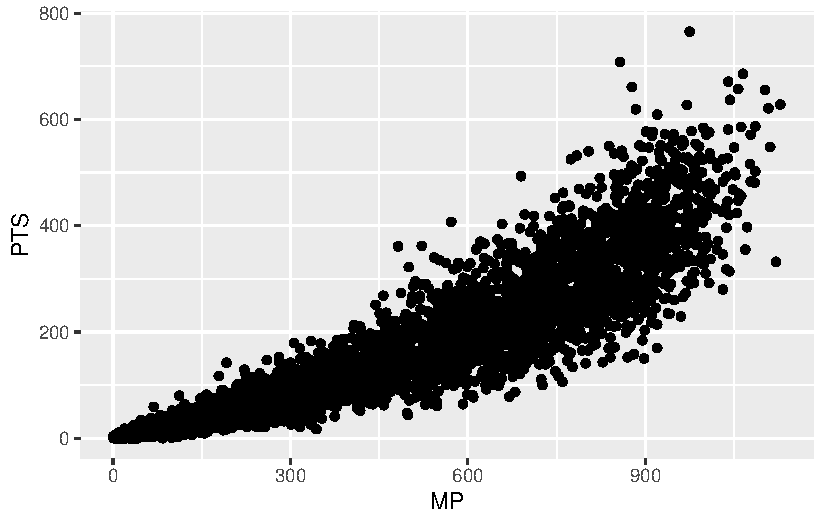
\includegraphics{./simulations_files/figure-pdf/unnamed-chunk-4-1.pdf}

}

\end{figure}

\begin{Shaded}
\begin{Highlighting}[]
\FunctionTok{table}\NormalTok{(simulations)}
\end{Highlighting}
\end{Shaded}

\begin{verbatim}
simulations
  0   1   2   3   4   5   6   7   8   9  10  11 
  5  16  59 132 200 218 172  92  65  34   4   3 
\end{verbatim}

Short answer: Really weird. If you simulate 15 threes 1000 times,
sometimes you'll see them miss all of them, but only a few times -- five
times, in this case. Most of the time, the team won't go 0-15 even once.
So going ice cold is not totally out of the realm of random chance, but
it's highly unlikely.

\bookmarksetup{startatroot}

\hypertarget{intro-to-ggplot-with-bar-charts}{%
\chapter{Intro to ggplot with bar
charts}\label{intro-to-ggplot-with-bar-charts}}

With \texttt{ggplot2}, we dive into the world of programmatic data
visualization. The \texttt{ggplot2} library implements something called
the grammar of graphics. The main concepts are:

\begin{itemize}
\tightlist
\item
  aesthetics - which in this case means the data which we are going to
  plot
\item
  geometries - which means the shape the data is going to take
\item
  scales - which means any transformations we might make on the data
\item
  facets - which means how we might graph many elements of the same
  dataset in the same space
\item
  layers - which means how we might lay multiple geometries over top of
  each other to reveal new information.
\end{itemize}

Hadley Wickham, who is behind all of the libraries we have used in this
course to date, wrote about his layered grammar of graphics in
\href{http://byrneslab.net/classes/biol607/readings/wickham_layered-grammar.pdf}{this
2009 paper that is worth your time to read}.

Here are some \texttt{ggplot2} resources you'll want to keep handy:

\begin{itemize}
\tightlist
\item
  \href{http://ggplot2.tidyverse.org/reference/index.html}{The ggplot
  documentation}.
\item
  \href{http://www.cookbook-r.com/Graphs/}{The ggplot cookbook}
\end{itemize}

Let's dive in using data we've already seen before -- football
attendance. This workflow will represent a clear picture of what your
work in this class will be like for much of the rest of the semester.
One way to think of this workflow is that your R Notebook is now your
digital sketchbook, where you will try different types of visualizations
to find ones that work. Then, you will either write the code that adds
necessary and required parts to finish it, or you'll export your work
into a program like Illustrator to finish the work.

To begin, we'll use data we've seen before: college football attendance.

Now load the tidyverse.

\begin{Shaded}
\begin{Highlighting}[]
\FunctionTok{library}\NormalTok{(tidyverse)}
\end{Highlighting}
\end{Shaded}

And the data.

\begin{Shaded}
\begin{Highlighting}[]
\NormalTok{attendance }\OtherTok{\textless{}{-}} \FunctionTok{read\_csv}\NormalTok{(}\StringTok{\textquotesingle{}data/attendance.csv\textquotesingle{}}\NormalTok{)}
\end{Highlighting}
\end{Shaded}

\begin{verbatim}
Rows: 150 Columns: 8
-- Column specification --------------------------------------------------------
Delimiter: ","
chr (2): Institution, Conference
dbl (6): 2013, 2014, 2015, 2016, 2017, 2018

i Use `spec()` to retrieve the full column specification for this data.
i Specify the column types or set `show_col_types = FALSE` to quiet this message.
\end{verbatim}

First, let's get a top 10 list by announced attendance in the most
recent season we have data. We'll use the same tricks we used in the
filtering assignment.

\begin{Shaded}
\begin{Highlighting}[]
\NormalTok{attendance }\SpecialCharTok{|\textgreater{}} 
  \FunctionTok{arrange}\NormalTok{(}\FunctionTok{desc}\NormalTok{(}\StringTok{\textasciigrave{}}\AttributeTok{2018}\StringTok{\textasciigrave{}}\NormalTok{)) }\SpecialCharTok{|\textgreater{}} 
  \FunctionTok{top\_n}\NormalTok{(}\DecValTok{10}\NormalTok{) }\SpecialCharTok{|\textgreater{}} 
  \FunctionTok{select}\NormalTok{(Institution, }\StringTok{\textasciigrave{}}\AttributeTok{2018}\StringTok{\textasciigrave{}}\NormalTok{)}
\end{Highlighting}
\end{Shaded}

\begin{verbatim}
Selecting by 2018
\end{verbatim}

\begin{verbatim}
# A tibble: 10 x 2
   Institution `2018`
   <chr>        <dbl>
 1 Michigan    775156
 2 Penn St.    738396
 3 Ohio St.    713630
 4 Alabama     710931
 5 LSU         705733
 6 Texas A&M   698908
 7 Tennessee   650887
 8 Georgia     649222
 9 Nebraska    623240
10 Oklahoma    607146
\end{verbatim}

That looks good, so let's save it to a new data frame and use that data
frame instead going forward.

\begin{Shaded}
\begin{Highlighting}[]
\NormalTok{top10 }\OtherTok{\textless{}{-}}\NormalTok{ attendance }\SpecialCharTok{|\textgreater{}}
  \FunctionTok{arrange}\NormalTok{(}\FunctionTok{desc}\NormalTok{(}\StringTok{\textasciigrave{}}\AttributeTok{2018}\StringTok{\textasciigrave{}}\NormalTok{)) }\SpecialCharTok{|\textgreater{}} 
  \FunctionTok{top\_n}\NormalTok{(}\DecValTok{10}\NormalTok{) }\SpecialCharTok{|\textgreater{}} 
  \FunctionTok{select}\NormalTok{(Institution, }\StringTok{\textasciigrave{}}\AttributeTok{2018}\StringTok{\textasciigrave{}}\NormalTok{)}
\end{Highlighting}
\end{Shaded}

\begin{verbatim}
Selecting by 2018
\end{verbatim}

\hypertarget{the-bar-chart}{%
\section{The bar chart}\label{the-bar-chart}}

The easiest thing we can do is create a simple bar chart of our data.
\textbf{Bar charts show magnitude. They invite you to compare how much
more or less one thing is compared to others.}

We could, for instance, create a bar chart of the total attendance. To
do that, we simply tell \texttt{ggplot2} what our dataset is, what
element of the data we want to make the bar chart out of (which is the
aesthetic), and the geometry type (which is the geom). It looks like
this:

\texttt{ggplot()\ +\ geom\_bar(data=top10,\ aes(x=Institution))}

Note: top10 is our data, \texttt{aes} means aesthetics,
\texttt{x=Institution} explicitly tells \texttt{ggplot2} that our x
value -- our horizontal value -- is the Institution field from the data,
and then we add on the \texttt{geom\_bar()} as the geometry. And what do
we get when we run that?

\begin{Shaded}
\begin{Highlighting}[]
\FunctionTok{ggplot}\NormalTok{() }\SpecialCharTok{+} 
  \FunctionTok{geom\_bar}\NormalTok{(}
    \AttributeTok{data=}\NormalTok{top10, }
    \FunctionTok{aes}\NormalTok{(}\AttributeTok{x=}\NormalTok{Institution)}
\NormalTok{  )}
\end{Highlighting}
\end{Shaded}

\begin{figure}[H]

{\centering \includegraphics{./barcharts_files/figure-pdf/unnamed-chunk-6-1.pdf}

}

\end{figure}

We get \ldots{} weirdness. We expected to see bars of different sizes,
but we get all with a count of 1. What gives? Well, this is the default
behavior. What we have here is something called a histogram, where
\texttt{ggplot2} helpfully counted up the number of times the
Institution appears and counted them up. Since we only have one record
per Institution, the count is always 1. How do we fix this? By adding
\texttt{weight} to our aesthetic.

\begin{Shaded}
\begin{Highlighting}[]
\FunctionTok{ggplot}\NormalTok{() }\SpecialCharTok{+} 
  \FunctionTok{geom\_bar}\NormalTok{(}
    \AttributeTok{data=}\NormalTok{top10, }
    \FunctionTok{aes}\NormalTok{(}\AttributeTok{x=}\NormalTok{Institution, }\AttributeTok{weight=}\StringTok{\textasciigrave{}}\AttributeTok{2018}\StringTok{\textasciigrave{}}\NormalTok{)}
\NormalTok{  )}
\end{Highlighting}
\end{Shaded}

\begin{figure}[H]

{\centering \includegraphics{./barcharts_files/figure-pdf/unnamed-chunk-7-1.pdf}

}

\end{figure}

Closer. But \ldots{} what order is that in? And what happened to our
count numbers on the left? Why are they in scientific notation?

Let's deal with the ordering first. \texttt{ggplot2}'s default behavior
is to sort the data by the x axis variable. So it's in alphabetical
order. To change that, we have to \texttt{reorder} it. With
\texttt{reorder}, we first have to tell \texttt{ggplot} what we are
reordering, and then we have to tell it HOW we are reordering it. So
it's reorder(FIELD, SORTFIELD).

\begin{Shaded}
\begin{Highlighting}[]
\FunctionTok{ggplot}\NormalTok{() }\SpecialCharTok{+} 
  \FunctionTok{geom\_bar}\NormalTok{(}
    \AttributeTok{data=}\NormalTok{top10, }
    \FunctionTok{aes}\NormalTok{(}
      \AttributeTok{x=}\FunctionTok{reorder}\NormalTok{(Institution, }\StringTok{\textasciigrave{}}\AttributeTok{2018}\StringTok{\textasciigrave{}}\NormalTok{), }
      \AttributeTok{weight=}\StringTok{\textasciigrave{}}\AttributeTok{2018}\StringTok{\textasciigrave{}}
\NormalTok{      )}
\NormalTok{    )}
\end{Highlighting}
\end{Shaded}

\begin{figure}[H]

{\centering \includegraphics{./barcharts_files/figure-pdf/unnamed-chunk-8-1.pdf}

}

\end{figure}

Better. We can argue about if the right order is smallest to largest or
largest to smallest. But this gets us close. By the way, to sort it
largest to smallest, put a negative sign in front of the sort field.

\begin{Shaded}
\begin{Highlighting}[]
\FunctionTok{ggplot}\NormalTok{() }\SpecialCharTok{+} 
  \FunctionTok{geom\_bar}\NormalTok{(}
    \AttributeTok{data=}\NormalTok{top10, }
    \FunctionTok{aes}\NormalTok{(}
      \AttributeTok{x=}\FunctionTok{reorder}\NormalTok{(Institution, }\SpecialCharTok{{-}}\StringTok{\textasciigrave{}}\AttributeTok{2018}\StringTok{\textasciigrave{}}\NormalTok{), }
      \AttributeTok{weight=}\StringTok{\textasciigrave{}}\AttributeTok{2018}\StringTok{\textasciigrave{}}
\NormalTok{      )}
\NormalTok{    )}
\end{Highlighting}
\end{Shaded}

\begin{figure}[H]

{\centering \includegraphics{./barcharts_files/figure-pdf/unnamed-chunk-9-1.pdf}

}

\end{figure}

\hypertarget{scales}{%
\section{Scales}\label{scales}}

To fix the axis labels, we need try one of the other main elements of
the \texttt{ggplot2} library, which is transform a scale. More often
that not, that means doing something like putting it on a logarithmic
scale or some other kind of transformation. In this case, we're just
changing how it's represented. The default in \texttt{ggplot2} for large
values is to express them as scientific notation. Rarely ever is that
useful in our line of work. So we have to transform them into human
readable numbers.

The easiest way to do this is to use a library called \texttt{scales}
and it's already installed.

\begin{Shaded}
\begin{Highlighting}[]
\FunctionTok{library}\NormalTok{(scales)}
\end{Highlighting}
\end{Shaded}

\begin{verbatim}

Attaching package: 'scales'
\end{verbatim}

\begin{verbatim}
The following object is masked from 'package:purrr':

    discard
\end{verbatim}

\begin{verbatim}
The following object is masked from 'package:readr':

    col_factor
\end{verbatim}

To alter the scale, we add a piece to our plot with \texttt{+} and we
tell it which scale is getting altered and what kind of data it is. In
our case, our Y axis is what is needing to be altered, and it's
continuous data (meaning it can be any number between x and y, vs
discrete data which are categorical). So we need to add
\texttt{scale\_y\_continuous} and the information we want to pass it is
to alter the labels with a function called \texttt{comma}.

\begin{Shaded}
\begin{Highlighting}[]
\FunctionTok{ggplot}\NormalTok{() }\SpecialCharTok{+} 
  \FunctionTok{geom\_bar}\NormalTok{(}
    \AttributeTok{data=}\NormalTok{top10, }
    \FunctionTok{aes}\NormalTok{(}
      \AttributeTok{x=}\FunctionTok{reorder}\NormalTok{(Institution, }\SpecialCharTok{{-}}\StringTok{\textasciigrave{}}\AttributeTok{2018}\StringTok{\textasciigrave{}}\NormalTok{), }
      \AttributeTok{weight=}\StringTok{\textasciigrave{}}\AttributeTok{2018}\StringTok{\textasciigrave{}}
\NormalTok{      )}
\NormalTok{    ) }\SpecialCharTok{+} 
  \FunctionTok{scale\_y\_continuous}\NormalTok{(}\AttributeTok{labels=}\NormalTok{comma)}
\end{Highlighting}
\end{Shaded}

\begin{figure}[H]

{\centering \includegraphics{./barcharts_files/figure-pdf/unnamed-chunk-11-1.pdf}

}

\end{figure}

Better.

\hypertarget{styling}{%
\section{Styling}\label{styling}}

We are going to spend a lot more time on styling, but let's add some
simple labels to this with a new bit called \texttt{labs} which is short
for labels.

\begin{Shaded}
\begin{Highlighting}[]
\FunctionTok{ggplot}\NormalTok{() }\SpecialCharTok{+} 
  \FunctionTok{geom\_bar}\NormalTok{(}
    \AttributeTok{data=}\NormalTok{top10, }
    \FunctionTok{aes}\NormalTok{(}
      \AttributeTok{x=}\FunctionTok{reorder}\NormalTok{(Institution, }\SpecialCharTok{{-}}\StringTok{\textasciigrave{}}\AttributeTok{2018}\StringTok{\textasciigrave{}}\NormalTok{), }
      \AttributeTok{weight=}\StringTok{\textasciigrave{}}\AttributeTok{2018}\StringTok{\textasciigrave{}}\NormalTok{)}
\NormalTok{    ) }\SpecialCharTok{+} 
  \FunctionTok{scale\_y\_continuous}\NormalTok{(}\AttributeTok{labels=}\NormalTok{comma) }\SpecialCharTok{+} 
  \FunctionTok{labs}\NormalTok{(}
    \AttributeTok{title=}\StringTok{"Top 10 Football Programs By Attendance"}\NormalTok{, }
    \AttributeTok{x=}\StringTok{"School"}\NormalTok{, }
    \AttributeTok{y=}\StringTok{"Attendance"}
\NormalTok{)}
\end{Highlighting}
\end{Shaded}

\begin{figure}[H]

{\centering \includegraphics{./barcharts_files/figure-pdf/unnamed-chunk-12-1.pdf}

}

\end{figure}

The library has lots and lots of ways to alter the styling -- we can
programmatically control nearly every part of the look and feel of the
chart. One simple way is to apply themes in the library already. We do
that the same way we've done other things -- we add them. Here's the
light theme.

\begin{Shaded}
\begin{Highlighting}[]
\FunctionTok{ggplot}\NormalTok{() }\SpecialCharTok{+} 
  \FunctionTok{geom\_bar}\NormalTok{(}
    \AttributeTok{data=}\NormalTok{top10, }
    \FunctionTok{aes}\NormalTok{(}\AttributeTok{x=}\FunctionTok{reorder}\NormalTok{(Institution, }\SpecialCharTok{{-}}\StringTok{\textasciigrave{}}\AttributeTok{2018}\StringTok{\textasciigrave{}}\NormalTok{),}
        \AttributeTok{weight=}\StringTok{\textasciigrave{}}\AttributeTok{2018}\StringTok{\textasciigrave{}}\NormalTok{)) }\SpecialCharTok{+} 
  \FunctionTok{scale\_y\_continuous}\NormalTok{(}\AttributeTok{labels=}\NormalTok{comma) }\SpecialCharTok{+} 
  \FunctionTok{labs}\NormalTok{(}
    \AttributeTok{title=}\StringTok{"Top 10 Football Programs By Attendance"}\NormalTok{, }
    \AttributeTok{x=}\StringTok{"School"}\NormalTok{, }
    \AttributeTok{y=}\StringTok{"Attendance"}\NormalTok{) }\SpecialCharTok{+} 
  \FunctionTok{theme\_light}\NormalTok{()}
\end{Highlighting}
\end{Shaded}

\begin{figure}[H]

{\centering 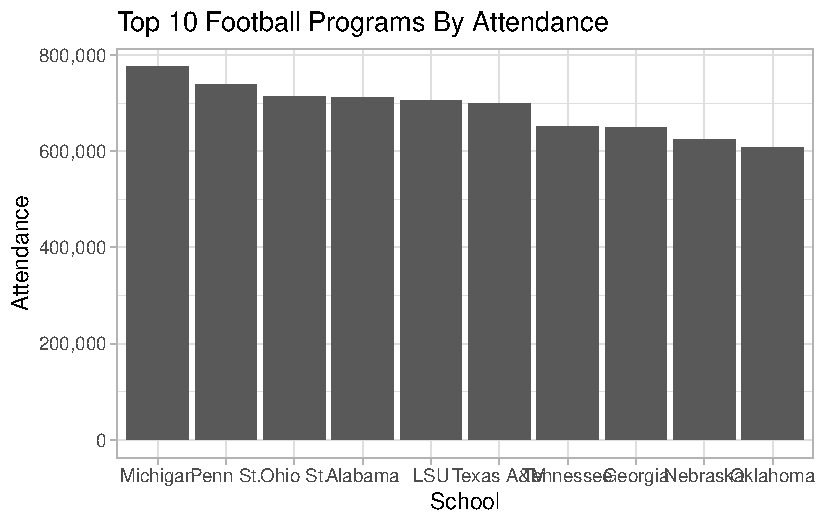
\includegraphics{./barcharts_files/figure-pdf/unnamed-chunk-13-1.pdf}

}

\end{figure}

Or the minimal theme:

\begin{Shaded}
\begin{Highlighting}[]
\FunctionTok{ggplot}\NormalTok{() }\SpecialCharTok{+} 
  \FunctionTok{geom\_bar}\NormalTok{(}
    \AttributeTok{data=}\NormalTok{top10, }
    \FunctionTok{aes}\NormalTok{(}\AttributeTok{x=}\FunctionTok{reorder}\NormalTok{(Institution, }\SpecialCharTok{{-}}\StringTok{\textasciigrave{}}\AttributeTok{2018}\StringTok{\textasciigrave{}}\NormalTok{),}
        \AttributeTok{weight=}\StringTok{\textasciigrave{}}\AttributeTok{2018}\StringTok{\textasciigrave{}}\NormalTok{)) }\SpecialCharTok{+} 
  \FunctionTok{scale\_y\_continuous}\NormalTok{(}\AttributeTok{labels=}\NormalTok{comma) }\SpecialCharTok{+} 
  \FunctionTok{labs}\NormalTok{(}
    \AttributeTok{title=}\StringTok{"Top 10 Football Programs By Attendance"}\NormalTok{, }
    \AttributeTok{x=}\StringTok{"School"}\NormalTok{, }
    \AttributeTok{y=}\StringTok{"Attendance"}\NormalTok{) }\SpecialCharTok{+} 
  \FunctionTok{theme\_minimal}\NormalTok{()}
\end{Highlighting}
\end{Shaded}

\begin{figure}[H]

{\centering \includegraphics{./barcharts_files/figure-pdf/unnamed-chunk-14-1.pdf}

}

\end{figure}

Later on, we'll write our own themes. For now, the built in ones will
get us closer to something that looks good.

\hypertarget{one-last-trick-coord-flip}{%
\section{One last trick: coord flip}\label{one-last-trick-coord-flip}}

Sometimes, we don't want vertical bars. Maybe we think this would look
better horizontal. How do we do that? By adding \texttt{coord\_flip()}
to our code. It does what it says -- it inverts the coordinates of the
figures.

\begin{Shaded}
\begin{Highlighting}[]
\FunctionTok{ggplot}\NormalTok{() }\SpecialCharTok{+} 
  \FunctionTok{geom\_bar}\NormalTok{(}
    \AttributeTok{data=}\NormalTok{top10, }
    \FunctionTok{aes}\NormalTok{(}\AttributeTok{x=}\FunctionTok{reorder}\NormalTok{(Institution, }\SpecialCharTok{{-}}\StringTok{\textasciigrave{}}\AttributeTok{2018}\StringTok{\textasciigrave{}}\NormalTok{),}
        \AttributeTok{weight=}\StringTok{\textasciigrave{}}\AttributeTok{2018}\StringTok{\textasciigrave{}}\NormalTok{)) }\SpecialCharTok{+} 
  \FunctionTok{scale\_y\_continuous}\NormalTok{(}\AttributeTok{labels=}\NormalTok{comma) }\SpecialCharTok{+} 
  \FunctionTok{labs}\NormalTok{(}
    \AttributeTok{title=}\StringTok{"Top 10 Football Programs By Attendance"}\NormalTok{, }
    \AttributeTok{x=}\StringTok{"School"}\NormalTok{, }
    \AttributeTok{y=}\StringTok{"Attendance"}\NormalTok{) }\SpecialCharTok{+} 
  \FunctionTok{theme\_minimal}\NormalTok{() }\SpecialCharTok{+} 
  \FunctionTok{coord\_flip}\NormalTok{()}
\end{Highlighting}
\end{Shaded}

\begin{figure}[H]

{\centering \includegraphics{./barcharts_files/figure-pdf/unnamed-chunk-15-1.pdf}

}

\end{figure}

\bookmarksetup{startatroot}

\hypertarget{stacked-bar-charts}{%
\chapter{Stacked bar charts}\label{stacked-bar-charts}}

One of the elements of data visualization excellence is \textbf{inviting
comparison}. Often that comes in showing \textbf{what proportion a thing
is in relation to the whole thing}. With bar charts, we're showing
magnitude of the whole thing. If we have information about the parts of
the whole, \textbf{we can stack them on top of each other to compare
them, showing both the whole and the components}. And it's a simple
change to what we've already done.

We're going to use a dataset of college basketball games from this past
season.

Load the tidyverse.

\begin{Shaded}
\begin{Highlighting}[]
\FunctionTok{library}\NormalTok{(tidyverse)}
\end{Highlighting}
\end{Shaded}

And the data.

\begin{Shaded}
\begin{Highlighting}[]
\NormalTok{games }\OtherTok{\textless{}{-}} \FunctionTok{read\_csv}\NormalTok{(}\StringTok{"data/logs22.csv"}\NormalTok{)}
\end{Highlighting}
\end{Shaded}

\begin{verbatim}
Rows: 10775 Columns: 48
-- Column specification --------------------------------------------------------
Delimiter: ","
chr   (8): Season, TeamFull, Opponent, HomeAway, W_L, URL, Conference, Team
dbl  (39): Game, TeamScore, OpponentScore, TeamFG, TeamFGA, TeamFGPCT, Team3...
date  (1): Date

i Use `spec()` to retrieve the full column specification for this data.
i Specify the column types or set `show_col_types = FALSE` to quiet this message.
\end{verbatim}

What we have here is every game in college football this season. The
question we want to answer is this: Who had the most prolific offenses
in the Big Ten? And how did they get there?

So to make this chart, we have to just add one thing to a bar chart like
we did in the previous chapter. However, it's not that simple.

We have game data, and we need season data. To get that, we need to do
some group by and sum work. And since we're only interested in the Big
Ten, we have some filtering to do too. For this, we're going to measure
offensive production by rushing yards and passing yards. So if we have
all the games a team played, and the rushing and passing yards for each
of those games, what we need to do to get the season totals is just add
them up.

\begin{Shaded}
\begin{Highlighting}[]
\NormalTok{games }\SpecialCharTok{|\textgreater{}} 
  \FunctionTok{group\_by}\NormalTok{(Conference, Team) }\SpecialCharTok{|\textgreater{}} 
  \FunctionTok{summarise}\NormalTok{(}
    \AttributeTok{SeasonOffRebounds =} \FunctionTok{sum}\NormalTok{(TeamOffRebounds),}
    \AttributeTok{SeasonTotalRebounds =} \FunctionTok{sum}\NormalTok{(TeamTotalRebounds)}
\NormalTok{  ) }\SpecialCharTok{|\textgreater{}}
  \FunctionTok{mutate}\NormalTok{(}
    \AttributeTok{SeasonDefRebounds =}\NormalTok{ SeasonTotalRebounds }\SpecialCharTok{{-}}\NormalTok{ SeasonOffRebounds}
\NormalTok{  ) }\SpecialCharTok{|\textgreater{}} 
  \FunctionTok{select}\NormalTok{(}
    \SpecialCharTok{{-}}\NormalTok{SeasonTotalRebounds}
\NormalTok{  ) }\SpecialCharTok{|\textgreater{}} 
  \FunctionTok{filter}\NormalTok{(Conference }\SpecialCharTok{==} \StringTok{"Big Ten"}\NormalTok{)}
\end{Highlighting}
\end{Shaded}

\begin{verbatim}
# A tibble: 14 x 4
# Groups:   Conference [1]
   Conference Team           SeasonOffRebounds SeasonDefRebounds
   <chr>      <chr>                      <dbl>             <dbl>
 1 Big Ten    Illinois                     300               764
 2 Big Ten    Indiana                      228               770
 3 Big Ten    Iowa                         333               742
 4 Big Ten    Maryland                     256               767
 5 Big Ten    Michigan                     265               721
 6 Big Ten    Michigan State               268               774
 7 Big Ten    Minnesota                    132               674
 8 Big Ten    Nebraska                     196               762
 9 Big Ten    Northwestern                 226               715
10 Big Ten    Ohio State                   225               706
11 Big Ten    Penn State                   224               707
12 Big Ten    Purdue                       295               794
13 Big Ten    Rutgers                      267               715
14 Big Ten    Wisconsin                    240               730
\end{verbatim}

By looking at this, we can see we got what we needed. We have 14 teams
and numbers that look like season totals for two types of rebounds. Save
that to a new dataframe.

\begin{Shaded}
\begin{Highlighting}[]
\NormalTok{games }\SpecialCharTok{|\textgreater{}} 
  \FunctionTok{group\_by}\NormalTok{(Conference, Team) }\SpecialCharTok{|\textgreater{}} 
  \FunctionTok{summarise}\NormalTok{(}
    \AttributeTok{SeasonOffRebounds =} \FunctionTok{sum}\NormalTok{(TeamOffRebounds),}
    \AttributeTok{SeasonTotalRebounds =} \FunctionTok{sum}\NormalTok{(TeamTotalRebounds)}
\NormalTok{  ) }\SpecialCharTok{|\textgreater{}}
  \FunctionTok{mutate}\NormalTok{(}
    \AttributeTok{SeasonDefRebounds =}\NormalTok{ SeasonTotalRebounds }\SpecialCharTok{{-}}\NormalTok{ SeasonOffRebounds}
\NormalTok{  ) }\SpecialCharTok{|\textgreater{}} 
  \FunctionTok{select}\NormalTok{(}
    \SpecialCharTok{{-}}\NormalTok{SeasonTotalRebounds}
\NormalTok{  ) }\SpecialCharTok{|\textgreater{}} 
  \FunctionTok{filter}\NormalTok{(Conference }\SpecialCharTok{==} \StringTok{"Big Ten"}\NormalTok{) }\OtherTok{{-}\textgreater{}}\NormalTok{ rebounds}
\end{Highlighting}
\end{Shaded}

Now, the problem we have is that ggplot wants long data and this data is
wide. So we need to use \texttt{tidyr} to make it long, just like we did
in the transforming data chapter.

\begin{Shaded}
\begin{Highlighting}[]
\NormalTok{rebounds }\SpecialCharTok{|\textgreater{}} 
  \FunctionTok{pivot\_longer}\NormalTok{(}
    \AttributeTok{cols=}\FunctionTok{starts\_with}\NormalTok{(}\StringTok{"Season"}\NormalTok{), }
    \AttributeTok{names\_to=}\StringTok{"Type"}\NormalTok{, }
    \AttributeTok{values\_to=}\StringTok{"Rebounds"}\NormalTok{)}
\end{Highlighting}
\end{Shaded}

\begin{verbatim}
# A tibble: 28 x 4
# Groups:   Conference [1]
   Conference Team     Type              Rebounds
   <chr>      <chr>    <chr>                <dbl>
 1 Big Ten    Illinois SeasonOffRebounds      300
 2 Big Ten    Illinois SeasonDefRebounds      764
 3 Big Ten    Indiana  SeasonOffRebounds      228
 4 Big Ten    Indiana  SeasonDefRebounds      770
 5 Big Ten    Iowa     SeasonOffRebounds      333
 6 Big Ten    Iowa     SeasonDefRebounds      742
 7 Big Ten    Maryland SeasonOffRebounds      256
 8 Big Ten    Maryland SeasonDefRebounds      767
 9 Big Ten    Michigan SeasonOffRebounds      265
10 Big Ten    Michigan SeasonDefRebounds      721
# i 18 more rows
\end{verbatim}

What you can see now is that we have two rows for each team: One for
rushing yards, one for passing yards. This is what ggplot needs. Save it
to a new dataframe.

\begin{Shaded}
\begin{Highlighting}[]
\NormalTok{rebounds }\SpecialCharTok{|\textgreater{}} 
  \FunctionTok{pivot\_longer}\NormalTok{(}
    \AttributeTok{cols=}\FunctionTok{starts\_with}\NormalTok{(}\StringTok{"Season"}\NormalTok{), }
    \AttributeTok{names\_to=}\StringTok{"Type"}\NormalTok{, }
    \AttributeTok{values\_to=}\StringTok{"Rebounds"}\NormalTok{) }\OtherTok{{-}\textgreater{}}\NormalTok{ reboundswide}
\end{Highlighting}
\end{Shaded}

Building on what we learned in the last chapter, we know we can turn
this into a bar chart with an x value, a weight and a geom\_bar. What we
are going to add is a \texttt{fill}. The \texttt{fill} will stack bars
on each other based on which element it is. In this case, we can fill
the bar by Type, which means it will stack the number of rushing yards
on top of passing yards and we can see how they compare.

\begin{Shaded}
\begin{Highlighting}[]
\FunctionTok{ggplot}\NormalTok{() }\SpecialCharTok{+} 
  \FunctionTok{geom\_bar}\NormalTok{(}
    \AttributeTok{data=}\NormalTok{reboundswide, }
    \FunctionTok{aes}\NormalTok{(}\AttributeTok{x=}\NormalTok{Team, }\AttributeTok{weight=}\NormalTok{Rebounds, }\AttributeTok{fill=}\NormalTok{Type)) }\SpecialCharTok{+} 
  \FunctionTok{coord\_flip}\NormalTok{()}
\end{Highlighting}
\end{Shaded}

\begin{figure}[H]

{\centering 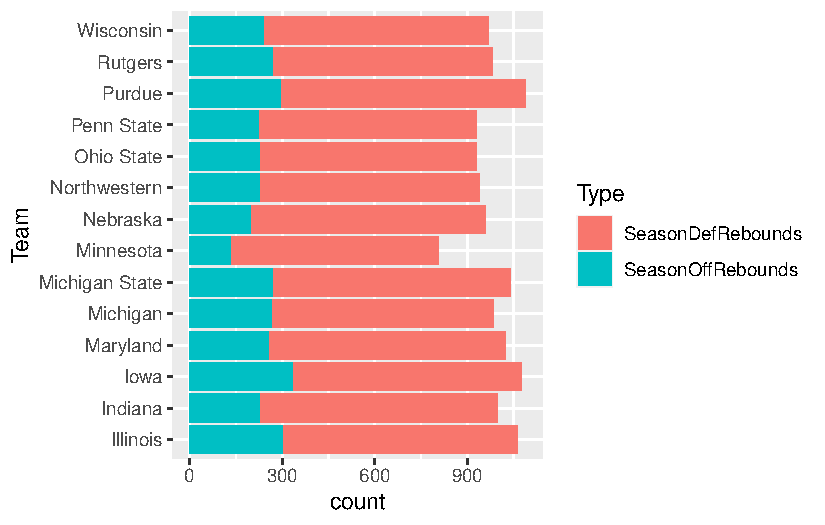
\includegraphics{./stackedbars_files/figure-pdf/unnamed-chunk-8-1.pdf}

}

\end{figure}

What's the problem with this chart?

There's a couple of things, one of which we'll deal with now: The
ordering is alphabetical (from the bottom up). So let's \texttt{reorder}
the teams by Rebounds.

\begin{Shaded}
\begin{Highlighting}[]
\FunctionTok{ggplot}\NormalTok{() }\SpecialCharTok{+} 
  \FunctionTok{geom\_bar}\NormalTok{(}
    \AttributeTok{data=}\NormalTok{reboundswide, }
    \FunctionTok{aes}\NormalTok{(}\AttributeTok{x=}\FunctionTok{reorder}\NormalTok{(Team, Rebounds), }
        \AttributeTok{weight=}\NormalTok{Rebounds, }
        \AttributeTok{fill=}\NormalTok{Type)) }\SpecialCharTok{+} 
  \FunctionTok{coord\_flip}\NormalTok{()}
\end{Highlighting}
\end{Shaded}

\begin{figure}[H]

{\centering 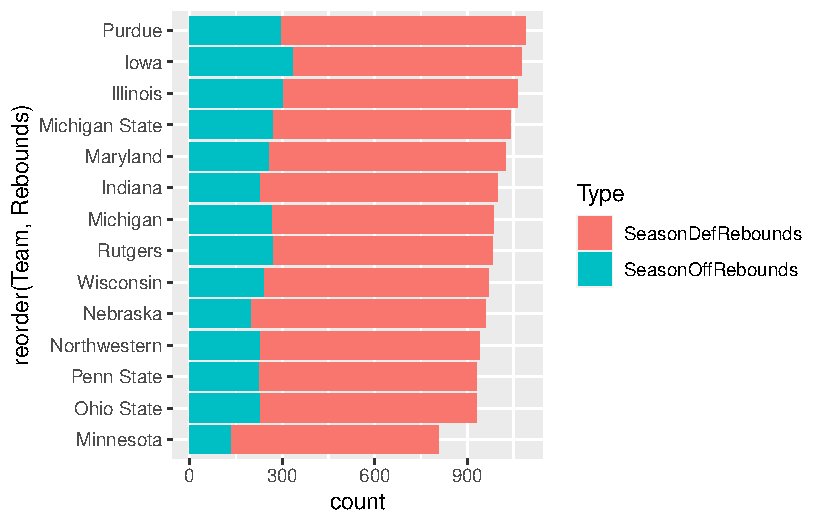
\includegraphics{./stackedbars_files/figure-pdf/unnamed-chunk-9-1.pdf}

}

\end{figure}

And just like that \ldots{} Purdue comes out on top? Huh. And look who
is not last.

\bookmarksetup{startatroot}

\hypertarget{circular-bar-charts}{%
\chapter{Circular bar charts}\label{circular-bar-charts}}

At the 27:36 mark in the
\href{https://www.omaha.com/sports/podcasts/half-court-press/half-court-press-creighton-cruises-in-opener-nebraska-stunned-in/article_67081a35-3a8f-5e9e-ae67-e88fcacbb362.html}{Half
Court Podcast}, former Omaha World Herald Writer Chris Heady said
``November basketball doesn't matter, but it shows you where you are.''

It's a tempting phrase to believe, especially a day after Nebraska lost
the first game of the Fred Hoiberg era at home to a baseball school, UC
Riverside. And it wasn't close. The Huskers, because of a total roster
turnover, were a complete mystery before the game. And what happened
during it wasn't pretty, so there was a little soul searching going on
in Lincoln.

But does November basketball really not matter?

Let's look, using a new form of chart called a circular bar plot. It's a
chart type that combines several forms we've used before: bar charts to
show magnitude, stacked bar charts to show proportion, but we're going
to add bending the chart around a circle to add some visual
interstingness to it. We're also going to use time as an x-axis value to
make a not subtle circle of time reference -- a common technique with
circular bar charts.

We'll use a dataset of every college basketball game last season.

Load your libraries.

\begin{Shaded}
\begin{Highlighting}[]
\FunctionTok{library}\NormalTok{(tidyverse)}
\FunctionTok{library}\NormalTok{(lubridate)}
\end{Highlighting}
\end{Shaded}

And load your data.

\begin{Shaded}
\begin{Highlighting}[]
\NormalTok{logs }\OtherTok{\textless{}{-}} \FunctionTok{read\_csv}\NormalTok{(}\StringTok{"data/logs20.csv"}\NormalTok{)}
\end{Highlighting}
\end{Shaded}

\begin{verbatim}
Rows: 11097 Columns: 43
-- Column specification --------------------------------------------------------
Delimiter: ","
chr   (6): HomeAway, Opponent, W_L, Team, Conference, season
dbl  (35): Game, TeamScore, OpponentScore, TeamFG, TeamFGA, TeamFGPCT, Team3...
lgl   (1): Blank
date  (1): Date

i Use `spec()` to retrieve the full column specification for this data.
i Specify the column types or set `show_col_types = FALSE` to quiet this message.
\end{verbatim}

\hypertarget{does-november-basketball-matter}{%
\section{Does November basketball
matter?}\label{does-november-basketball-matter}}

So let's test the notion of November Basketball Doesn't Matter. What
matters in basketball? Let's start simple: Wins.

Sports Reference's win columns are weird, so we need to scan through
them and find W and L and we'll give them numbers using
\texttt{case\_when}. I'm also going to filter out tournament basketball.

\begin{Shaded}
\begin{Highlighting}[]
\NormalTok{winlosslogs }\OtherTok{\textless{}{-}}\NormalTok{ logs }\SpecialCharTok{|\textgreater{}} 
  \FunctionTok{mutate}\NormalTok{(}\AttributeTok{winloss =} \FunctionTok{case\_when}\NormalTok{(}
    \FunctionTok{grepl}\NormalTok{(}\StringTok{"W"}\NormalTok{, W\_L) }\SpecialCharTok{\textasciitilde{}} \DecValTok{1}\NormalTok{, }
    \FunctionTok{grepl}\NormalTok{(}\StringTok{"L"}\NormalTok{, W\_L) }\SpecialCharTok{\textasciitilde{}} \DecValTok{0}\NormalTok{)}
\NormalTok{) }
\end{Highlighting}
\end{Shaded}

Now we can group by date and conference and sum up the wins. How many
wins by day does each conference get?

\begin{Shaded}
\begin{Highlighting}[]
\NormalTok{dates }\OtherTok{\textless{}{-}}\NormalTok{ winlosslogs }\SpecialCharTok{|\textgreater{}} 
  \FunctionTok{group\_by}\NormalTok{(Date, Conference) }\SpecialCharTok{|\textgreater{}} 
  \FunctionTok{summarise}\NormalTok{(}\AttributeTok{wins =} \FunctionTok{sum}\NormalTok{(winloss))}
\end{Highlighting}
\end{Shaded}

\begin{verbatim}
`summarise()` has grouped output by 'Date'. You can override using the
`.groups` argument.
\end{verbatim}

Earlier, we did stacked bar charts. We have what we need to do that now.

\begin{Shaded}
\begin{Highlighting}[]
\FunctionTok{ggplot}\NormalTok{() }\SpecialCharTok{+} 
  \FunctionTok{geom\_bar}\NormalTok{(}
    \AttributeTok{data=}\NormalTok{dates, }
    \FunctionTok{aes}\NormalTok{(}\AttributeTok{x=}\NormalTok{Date, }\AttributeTok{weight=}\NormalTok{wins, }\AttributeTok{fill=}\NormalTok{Conference)}
\NormalTok{    ) }\SpecialCharTok{+} 
  \FunctionTok{theme\_minimal}\NormalTok{()}
\end{Highlighting}
\end{Shaded}

\begin{figure}[H]

{\centering \includegraphics{./circularbarcharts_files/figure-pdf/unnamed-chunk-6-1.pdf}

}

\end{figure}

Eeek. This is already looking not great. But to make it a circular bar
chart, we add \texttt{coord\_polar()} to our chart.

\begin{Shaded}
\begin{Highlighting}[]
\FunctionTok{ggplot}\NormalTok{() }\SpecialCharTok{+} 
  \FunctionTok{geom\_bar}\NormalTok{(}
    \AttributeTok{data=}\NormalTok{dates, }
    \FunctionTok{aes}\NormalTok{(}\AttributeTok{x=}\NormalTok{Date, }\AttributeTok{weight=}\NormalTok{wins, }\AttributeTok{fill=}\NormalTok{Conference)}
\NormalTok{    ) }\SpecialCharTok{+} 
  \FunctionTok{theme\_minimal}\NormalTok{() }\SpecialCharTok{+} 
  \FunctionTok{coord\_polar}\NormalTok{()}
\end{Highlighting}
\end{Shaded}

\begin{figure}[H]

{\centering \includegraphics{./circularbarcharts_files/figure-pdf/unnamed-chunk-7-1.pdf}

}

\end{figure}

Based on that, the day is probably too thin a slice, and there's way too
many conferences in college basketball. Let's group this by months and
filter out all but the power five conferences.

\begin{Shaded}
\begin{Highlighting}[]
\NormalTok{p5 }\OtherTok{\textless{}{-}} \FunctionTok{c}\NormalTok{(}\StringTok{"SEC"}\NormalTok{, }\StringTok{"Big Ten"}\NormalTok{, }\StringTok{"Pac{-}12"}\NormalTok{, }\StringTok{"Big 12"}\NormalTok{, }\StringTok{"ACC"}\NormalTok{)}
\end{Highlighting}
\end{Shaded}

To get months, we're going to use a function in the library
\texttt{lubridate} called \texttt{floor\_date}, which combine with
mutate will give us a field of just months.

\begin{Shaded}
\begin{Highlighting}[]
\NormalTok{wins }\OtherTok{\textless{}{-}}\NormalTok{ winlosslogs }\SpecialCharTok{|\textgreater{}} 
  \FunctionTok{mutate}\NormalTok{(}\AttributeTok{month =} \FunctionTok{floor\_date}\NormalTok{(Date, }\AttributeTok{unit=}\StringTok{"months"}\NormalTok{)) }\SpecialCharTok{|\textgreater{}} 
  \FunctionTok{group\_by}\NormalTok{(month, Conference) }\SpecialCharTok{|\textgreater{}} 
  \FunctionTok{summarise}\NormalTok{(}\AttributeTok{wins=}\FunctionTok{sum}\NormalTok{(winloss)) }\SpecialCharTok{|\textgreater{}} 
  \FunctionTok{filter}\NormalTok{(Conference }\SpecialCharTok{\%in\%}\NormalTok{ p5) }
\end{Highlighting}
\end{Shaded}

\begin{verbatim}
`summarise()` has grouped output by 'month'. You can override using the
`.groups` argument.
\end{verbatim}

Now we can use wins to make our circular bar chart of wins by month in
the Power Five.

\begin{Shaded}
\begin{Highlighting}[]
\FunctionTok{ggplot}\NormalTok{() }\SpecialCharTok{+} 
  \FunctionTok{geom\_bar}\NormalTok{(}
    \AttributeTok{data=}\NormalTok{wins, }
    \FunctionTok{aes}\NormalTok{(}\AttributeTok{x=}\NormalTok{month, }\AttributeTok{weight=}\NormalTok{wins, }\AttributeTok{fill=}\NormalTok{Conference)}
\NormalTok{    ) }\SpecialCharTok{+} 
  \FunctionTok{theme\_minimal}\NormalTok{() }\SpecialCharTok{+} 
  \FunctionTok{coord\_polar}\NormalTok{()}
\end{Highlighting}
\end{Shaded}

\begin{figure}[H]

{\centering \includegraphics{./circularbarcharts_files/figure-pdf/unnamed-chunk-10-1.pdf}

}

\end{figure}

Yikes. That looks a lot like a broken pie chart. So months are too thick
of a slice. Let's use weeks in our floor date to see what that gives us.

\begin{Shaded}
\begin{Highlighting}[]
\NormalTok{wins }\OtherTok{\textless{}{-}}\NormalTok{ winlosslogs }\SpecialCharTok{|\textgreater{}} 
  \FunctionTok{mutate}\NormalTok{(}\AttributeTok{week =} \FunctionTok{floor\_date}\NormalTok{(Date, }\AttributeTok{unit=}\StringTok{"weeks"}\NormalTok{)) }\SpecialCharTok{|\textgreater{}} 
  \FunctionTok{group\_by}\NormalTok{(week, Conference) }\SpecialCharTok{|\textgreater{}} 
  \FunctionTok{summarise}\NormalTok{(}\AttributeTok{wins=}\FunctionTok{sum}\NormalTok{(winloss)) }\SpecialCharTok{|\textgreater{}} 
  \FunctionTok{filter}\NormalTok{(Conference }\SpecialCharTok{\%in\%}\NormalTok{ p5) }
\end{Highlighting}
\end{Shaded}

\begin{verbatim}
`summarise()` has grouped output by 'week'. You can override using the
`.groups` argument.
\end{verbatim}

\begin{Shaded}
\begin{Highlighting}[]
\FunctionTok{ggplot}\NormalTok{() }\SpecialCharTok{+} 
  \FunctionTok{geom\_bar}\NormalTok{(}
    \AttributeTok{data=}\NormalTok{wins, }
    \FunctionTok{aes}\NormalTok{(}\AttributeTok{x=}\NormalTok{week, }\AttributeTok{weight=}\NormalTok{wins, }\AttributeTok{fill=}\NormalTok{Conference)}
\NormalTok{    ) }\SpecialCharTok{+} 
  \FunctionTok{theme\_minimal}\NormalTok{() }\SpecialCharTok{+} 
  \FunctionTok{coord\_polar}\NormalTok{()}
\end{Highlighting}
\end{Shaded}

\begin{figure}[H]

{\centering \includegraphics{./circularbarcharts_files/figure-pdf/unnamed-chunk-12-1.pdf}

}

\end{figure}

That looks better. But what does it say? Does November basketball
matter? What this is saying is \ldots{} yeah, it kinda does. The reason?
Lots of wins get piled up in November and December, during
non-conference play. So if you are a team with NCAA tournament dreams,
you need to win games in November to make sure your tournament resume is
where it needs to be come March. Does an individual win or loss matter?
Probably not. But your record in November does.

\hypertarget{does-it-show-you-where-you-are}{%
\section{Does it show you where you
are?}\label{does-it-show-you-where-you-are}}

So here is the problem we have:

\begin{enumerate}
\def\labelenumi{\arabic{enumi}.}
\tightlist
\item
  We have data for every game. In the past, we were able to calculate
  the team wins and losses because the way the data records them is the
  Team is the main team, and they win or lose. The Opponent is recorded,
  but the Opponent has the mirror image of this game as well, where they
  are the Team. So essentially every game is in here twice -- one for
  each team that plays in the game.
\item
  We need to attach the Opponent's winning percentage to each game so we
  can decide if it's a quality win for Team.
\item
  The Team name is not an exact copy of the Team name. So we can't join
  them using it.
\end{enumerate}

So what we have to do is invert the process that we've done before. We
need to group by the Opponent -- because the names will be consistent
then -- and we need to invert the wins and losses. A win in the W\_L
column is a win for the Team. That means each loss in the W\_L column is
a WIN for the Opponent.

Once we invert, the data looks very similar to what we've done before.
One other thing: I noticed there's some tournament games in here, so the
filter at the end strips them out.

\begin{Shaded}
\begin{Highlighting}[]
\NormalTok{oppwinlosslogs }\OtherTok{\textless{}{-}}\NormalTok{ logs }\SpecialCharTok{|\textgreater{}} 
  \FunctionTok{mutate}\NormalTok{(}\AttributeTok{winloss =} \FunctionTok{case\_when}\NormalTok{(}
    \FunctionTok{grepl}\NormalTok{(}\StringTok{"W"}\NormalTok{, W\_L) }\SpecialCharTok{\textasciitilde{}} \DecValTok{0}\NormalTok{, }
    \FunctionTok{grepl}\NormalTok{(}\StringTok{"L"}\NormalTok{, W\_L) }\SpecialCharTok{\textasciitilde{}} \DecValTok{1}\NormalTok{)}
\NormalTok{) }\SpecialCharTok{|\textgreater{}} 
  \FunctionTok{filter}\NormalTok{(Date }\SpecialCharTok{\textless{}} \StringTok{"2020{-}03{-}19"}\NormalTok{)}
\end{Highlighting}
\end{Shaded}

So now we have a dataframe called oppwinlosslogs that has an inverted
winloss column. So now we can group by the Opponent and sum the wins and
it will tell us how many games the Opponent won. We can also count the
wins and get a winning percentage.

\begin{Shaded}
\begin{Highlighting}[]
\NormalTok{oppwinlosslogs }\SpecialCharTok{|\textgreater{}} 
  \FunctionTok{group\_by}\NormalTok{(Opponent) }\SpecialCharTok{|\textgreater{}} 
  \FunctionTok{summarise}\NormalTok{(}\AttributeTok{games=}\FunctionTok{n}\NormalTok{(), }\AttributeTok{wins=}\FunctionTok{sum}\NormalTok{(winloss)) }\SpecialCharTok{|\textgreater{}} 
  \FunctionTok{mutate}\NormalTok{(}\AttributeTok{winpct =}\NormalTok{ wins}\SpecialCharTok{/}\NormalTok{games) }\OtherTok{{-}\textgreater{}}\NormalTok{ opprecord}
\end{Highlighting}
\end{Shaded}

Now we have a dataframe of 659 opponent winning records. Wait, what?
There's 353 teams in major college basketball, so why 659? If you look
through it, there's a bunch of teams playing lower level teams. Given
that they are lower level, they're likely cannon fodder and will lose
the game, and we're going to filter them out in a minute.

Now we can join the opponent winning percentage to our winlosslogs data
so we can answer our question about quality wins.

\begin{Shaded}
\begin{Highlighting}[]
\NormalTok{winlosslogs }\OtherTok{\textless{}{-}}\NormalTok{ logs }\SpecialCharTok{|\textgreater{}} 
  \FunctionTok{mutate}\NormalTok{(}\AttributeTok{winloss =} \FunctionTok{case\_when}\NormalTok{(}
    \FunctionTok{grepl}\NormalTok{(}\StringTok{"W"}\NormalTok{, W\_L) }\SpecialCharTok{\textasciitilde{}} \DecValTok{1}\NormalTok{, }
    \FunctionTok{grepl}\NormalTok{(}\StringTok{"L"}\NormalTok{, W\_L) }\SpecialCharTok{\textasciitilde{}} \DecValTok{0}\NormalTok{)}
\NormalTok{) }\SpecialCharTok{|\textgreater{}} 
  \FunctionTok{filter}\NormalTok{(Date }\SpecialCharTok{\textless{}} \StringTok{"2020{-}03{-}19"}\NormalTok{)}
\end{Highlighting}
\end{Shaded}

\begin{Shaded}
\begin{Highlighting}[]
\NormalTok{winlosslogs }\SpecialCharTok{|\textgreater{}} 
  \FunctionTok{left\_join}\NormalTok{(opprecord, }\AttributeTok{by=}\NormalTok{(}\StringTok{"Opponent"}\NormalTok{)) }\OtherTok{{-}\textgreater{}}\NormalTok{ winswithopppct}
\end{Highlighting}
\end{Shaded}

Now that we have a table called winswithopppct, we can filter out teams
non power 5 teams and teams that won less than 60 percent of their games
and run the same calculations in the book.

\begin{Shaded}
\begin{Highlighting}[]
\NormalTok{p5 }\OtherTok{\textless{}{-}} \FunctionTok{c}\NormalTok{(}\StringTok{"SEC"}\NormalTok{, }\StringTok{"Big Ten"}\NormalTok{, }\StringTok{"Pac{-}12"}\NormalTok{, }\StringTok{"Big 12"}\NormalTok{, }\StringTok{"ACC"}\NormalTok{)}
\end{Highlighting}
\end{Shaded}

\begin{Shaded}
\begin{Highlighting}[]
\NormalTok{winswithopppct }\SpecialCharTok{|\textgreater{}} 
  \FunctionTok{filter}\NormalTok{(winpct }\SpecialCharTok{\textgreater{}}\NormalTok{ .}\DecValTok{6}\NormalTok{) }\SpecialCharTok{|\textgreater{}} 
  \FunctionTok{mutate}\NormalTok{(}\AttributeTok{week =} \FunctionTok{floor\_date}\NormalTok{(Date, }\AttributeTok{unit=}\StringTok{"weeks"}\NormalTok{)) }\SpecialCharTok{|\textgreater{}} 
  \FunctionTok{group\_by}\NormalTok{(week, Conference) }\SpecialCharTok{|\textgreater{}} 
  \FunctionTok{summarise}\NormalTok{(}\AttributeTok{wins=}\FunctionTok{sum}\NormalTok{(winloss)) }\SpecialCharTok{|\textgreater{}} 
  \FunctionTok{filter}\NormalTok{(Conference }\SpecialCharTok{\%in\%}\NormalTok{ p5) }\OtherTok{{-}\textgreater{}}\NormalTok{ qualitywins}
\end{Highlighting}
\end{Shaded}

\begin{verbatim}
`summarise()` has grouped output by 'week'. You can override using the
`.groups` argument.
\end{verbatim}

Now with our dataframe called qualitywins, we can chart it again.

\begin{Shaded}
\begin{Highlighting}[]
\FunctionTok{ggplot}\NormalTok{() }\SpecialCharTok{+} 
  \FunctionTok{geom\_bar}\NormalTok{(}
    \AttributeTok{data=}\NormalTok{qualitywins, }
    \FunctionTok{aes}\NormalTok{(}\AttributeTok{x=}\NormalTok{week, }\AttributeTok{weight=}\NormalTok{wins, }\AttributeTok{fill=}\NormalTok{Conference)}
\NormalTok{    ) }\SpecialCharTok{+} 
  \FunctionTok{theme\_minimal}\NormalTok{() }\SpecialCharTok{+} 
  \FunctionTok{coord\_polar}\NormalTok{()}
\end{Highlighting}
\end{Shaded}

\begin{figure}[H]

{\centering 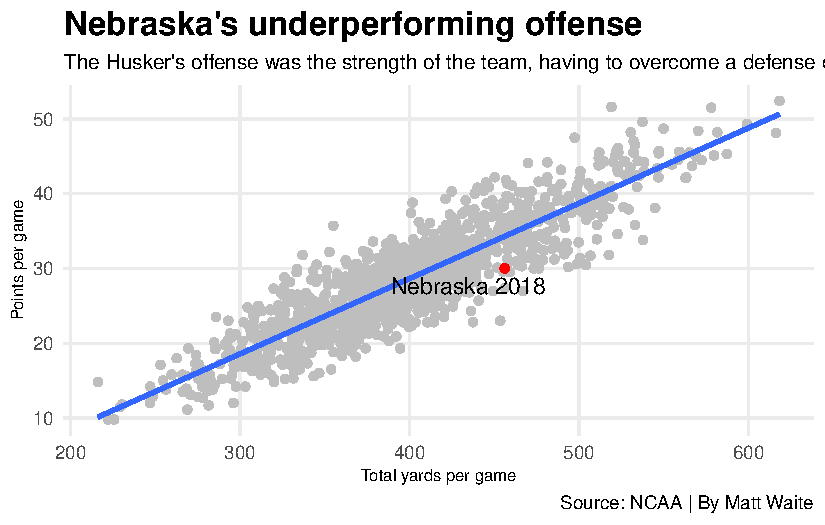
\includegraphics{./circularbarcharts_files/figure-pdf/unnamed-chunk-19-1.pdf}

}

\end{figure}

Look at this chart and compare it to the first one.

\bookmarksetup{startatroot}

\hypertarget{waffle-charts}{%
\chapter{Waffle charts}\label{waffle-charts}}

Pie charts are the devil. They should be an instant F in any data
visualization class. The problem? How carefully can you evaluate angles
and area? Unless they are blindingly obvious and only a few categories,
not well. If you've got 25 categories, how can you tell the difference
between 7 and 9 percent? You can't.

So let's introduce a better way: The Waffle Chart. Some call it a square
pie chart. I personally hate that. Waffles it is.

\textbf{A waffle chart is designed to show you parts of the whole --
proportionality}. How many yards on offense come from rushing or
passing. How many singles, doubles, triples and home runs make up a
teams hits. How many shots a basketball team takes are two pointers
versus three pointers.

First, install the library in the console. We want a newer version of
the \texttt{waffle} library than is in CRAN -- where you normally get
libraries from -- so copy and paste this into your console:

\texttt{install.packages("waffle")}

Now load it:

\begin{Shaded}
\begin{Highlighting}[]
\FunctionTok{library}\NormalTok{(waffle)}
\end{Highlighting}
\end{Shaded}

\hypertarget{making-waffles-with-vectors}{%
\section{Making waffles with
vectors}\label{making-waffles-with-vectors}}

Let's look at the debacle that was Nebraska vs.~Michigan State in fall
2021 in college football.
\href{https://www.espn.com/college-football/matchup?gameId=401282784}{Here's
the box score}, which we'll use for this part of the walkthrough.

Maybe the easiest way to do waffle charts, at least at first, is to make
vectors of your data and plug them in. To make a vector, we use the
\texttt{c} or concatenate function.

So let's look at offense. Rushing vs passing.

\begin{Shaded}
\begin{Highlighting}[]
\NormalTok{nu }\OtherTok{\textless{}{-}} \FunctionTok{c}\NormalTok{(}\StringTok{"Rushing"}\OtherTok{=}\DecValTok{187}\NormalTok{, }\StringTok{"Passing"}\OtherTok{=}\DecValTok{255}\NormalTok{)}
\NormalTok{ms }\OtherTok{\textless{}{-}} \FunctionTok{c}\NormalTok{(}\StringTok{"Rushing"}\OtherTok{=}\DecValTok{71}\NormalTok{, }\StringTok{"Passing"}\OtherTok{=}\DecValTok{183}\NormalTok{)}
\end{Highlighting}
\end{Shaded}

So what does the breakdown of the night look like?

The waffle library can break this down in a way that's easier on the
eyes than a pie chart. We call the library, add the data, specify the
number of rows, give it a title and an x value label, and to clean up a
quirk of the library, we've got to specify colors.

\begin{Shaded}
\begin{Highlighting}[]
\FunctionTok{waffle}\NormalTok{(}
\NormalTok{        nu, }
        \AttributeTok{rows =} \DecValTok{10}\NormalTok{, }
        \AttributeTok{title=}\StringTok{"Nebraska\textquotesingle{}s offense"}\NormalTok{, }
        \AttributeTok{xlab=}\StringTok{"1 square = 1 yard"}\NormalTok{, }
        \AttributeTok{colors =} \FunctionTok{c}\NormalTok{(}\StringTok{"black"}\NormalTok{, }\StringTok{"red"}\NormalTok{)}
\NormalTok{)}
\end{Highlighting}
\end{Shaded}

\begin{figure}[H]

{\centering 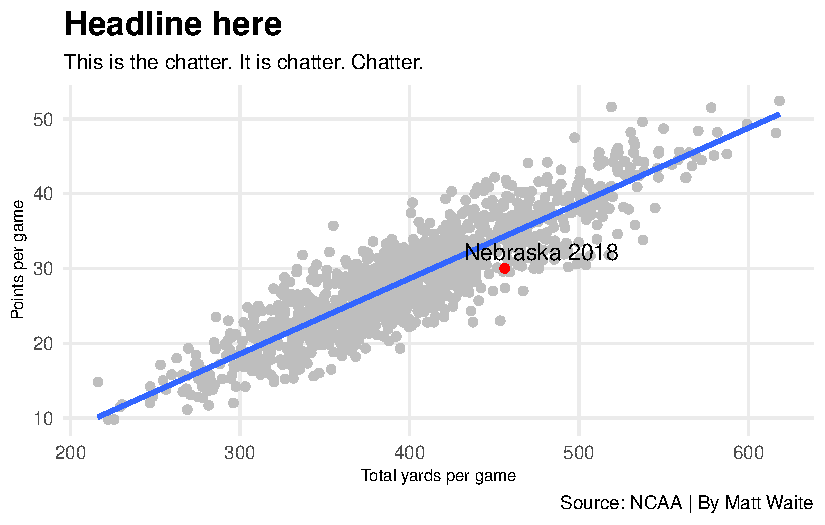
\includegraphics{./wafflecharts_files/figure-pdf/unnamed-chunk-3-1.pdf}

}

\end{figure}

Or, we could make this two teams in the same chart.

\begin{Shaded}
\begin{Highlighting}[]
\NormalTok{passing }\OtherTok{\textless{}{-}} \FunctionTok{c}\NormalTok{(}\StringTok{"Nebraska"}\OtherTok{=}\DecValTok{255}\NormalTok{, }\StringTok{"Mighigan State"}\OtherTok{=}\DecValTok{183}\NormalTok{)}
\end{Highlighting}
\end{Shaded}

\begin{Shaded}
\begin{Highlighting}[]
\FunctionTok{waffle}\NormalTok{(}
\NormalTok{        passing, }
        \AttributeTok{rows =} \DecValTok{10}\NormalTok{, }
        \AttributeTok{title=}\StringTok{"Nebraska vs Michigan State: passing"}\NormalTok{, }
        \AttributeTok{xlab=}\StringTok{"1 square = 1 yard"}\NormalTok{, }
        \AttributeTok{colors =} \FunctionTok{c}\NormalTok{(}\StringTok{"red"}\NormalTok{, }\StringTok{"black"}\NormalTok{)}
\NormalTok{)}
\end{Highlighting}
\end{Shaded}

\begin{figure}[H]

{\centering \includegraphics{./wafflecharts_files/figure-pdf/unnamed-chunk-5-1.pdf}

}

\end{figure}

So what does it look like if we compare the two teams using the two
vectors in the same chart? To do that -- and I am not making this up --
you have to create a waffle iron. Get it? Waffle charts? Iron?

\begin{Shaded}
\begin{Highlighting}[]
\FunctionTok{iron}\NormalTok{(}
 \FunctionTok{waffle}\NormalTok{(nu, }
        \AttributeTok{rows =} \DecValTok{10}\NormalTok{, }
        \AttributeTok{title=}\StringTok{"Nebraska\textquotesingle{}s offense"}\NormalTok{, }
        \AttributeTok{xlab=}\StringTok{"1 square = 1 yard"}\NormalTok{, }
        \AttributeTok{colors =} \FunctionTok{c}\NormalTok{(}\StringTok{"black"}\NormalTok{, }\StringTok{"red"}\NormalTok{)}
\NormalTok{        ),}
 \FunctionTok{waffle}\NormalTok{(ms, }
        \AttributeTok{rows =} \DecValTok{10}\NormalTok{, }
        \AttributeTok{title=}\StringTok{"Michigan State\textquotesingle{}s offense"}\NormalTok{, }
        \AttributeTok{xlab=}\StringTok{"1 square = 1 yard"}\NormalTok{, }
        \AttributeTok{colors =} \FunctionTok{c}\NormalTok{(}\StringTok{"black"}\NormalTok{, }\StringTok{"red"}\NormalTok{)}
\NormalTok{        )}
\NormalTok{)}
\end{Highlighting}
\end{Shaded}

\begin{figure}[H]

{\centering \includegraphics{./wafflecharts_files/figure-pdf/unnamed-chunk-6-1.pdf}

}

\end{figure}

What do you notice about this chart? Notice how the squares aren't the
same size? Well, Nebraska out-gained Michigan State by a long way
\ldots{} AND LOST. So the squares aren't the same size because the
numbers aren't the same. We can fix that by adding an unnamed padding
number so the number of yards add up to the same thing. Let's make the
total for everyone be 442, Nebraska's total yards of offense. So to do
that, we need to add a padding of 188 to Michigan State. REMEMBER: Don't
name it or it'll show up in the legend.

\begin{Shaded}
\begin{Highlighting}[]
\NormalTok{nu }\OtherTok{\textless{}{-}} \FunctionTok{c}\NormalTok{(}\StringTok{"Rushing"}\OtherTok{=}\DecValTok{187}\NormalTok{, }\StringTok{"Passing"}\OtherTok{=}\DecValTok{255}\NormalTok{)}
\NormalTok{ms }\OtherTok{\textless{}{-}} \FunctionTok{c}\NormalTok{(}\StringTok{"Rushing"}\OtherTok{=}\DecValTok{71}\NormalTok{, }\StringTok{"Passing"}\OtherTok{=}\DecValTok{183}\NormalTok{, }\DecValTok{188}\NormalTok{)}
\end{Highlighting}
\end{Shaded}

Now, in our waffle iron, if we don't give that padding a color, we'll
get an error. So we need to make it white. Which, given our white
background, means it will disappear.

\begin{Shaded}
\begin{Highlighting}[]
\FunctionTok{iron}\NormalTok{(}
 \FunctionTok{waffle}\NormalTok{(nu, }
        \AttributeTok{rows =} \DecValTok{10}\NormalTok{, }
        \AttributeTok{title=}\StringTok{"Nebraska\textquotesingle{}s offense"}\NormalTok{, }
        \AttributeTok{xlab=}\StringTok{"1 square = 1 yard"}\NormalTok{, }
        \AttributeTok{colors =} \FunctionTok{c}\NormalTok{(}\StringTok{"black"}\NormalTok{, }\StringTok{"red"}\NormalTok{)}
\NormalTok{        ),}
 \FunctionTok{waffle}\NormalTok{(ms, }
        \AttributeTok{rows =} \DecValTok{10}\NormalTok{, }
        \AttributeTok{title=}\StringTok{"Michigan State\textquotesingle{}s offense"}\NormalTok{, }
        \AttributeTok{xlab=}\StringTok{"1 square = 1 yard"}\NormalTok{, }
        \AttributeTok{colors =} \FunctionTok{c}\NormalTok{(}\StringTok{"dark green"}\NormalTok{, }\StringTok{"black"}\NormalTok{, }\StringTok{"white"}\NormalTok{)}
\NormalTok{        )}
\NormalTok{)}
\end{Highlighting}
\end{Shaded}

\begin{figure}[H]

{\centering \includegraphics{./wafflecharts_files/figure-pdf/unnamed-chunk-8-1.pdf}

}

\end{figure}

One last thing we can do is change the 1 square = 1 yard bit -- which
makes the squares really small in this case -- by dividing our vector.
Remember what you learned in Swirl about math on vectors?

\begin{Shaded}
\begin{Highlighting}[]
\FunctionTok{iron}\NormalTok{(}
 \FunctionTok{waffle}\NormalTok{(nu}\SpecialCharTok{/}\DecValTok{2}\NormalTok{, }
        \AttributeTok{rows =} \DecValTok{10}\NormalTok{, }
        \AttributeTok{title=}\StringTok{"Nebraska\textquotesingle{}s offense"}\NormalTok{, }
        \AttributeTok{xlab=}\StringTok{"1 square = 2 yards"}\NormalTok{, }
        \AttributeTok{colors =} \FunctionTok{c}\NormalTok{(}\StringTok{"black"}\NormalTok{, }\StringTok{"red"}\NormalTok{)}
\NormalTok{        ),}
 \FunctionTok{waffle}\NormalTok{(ms}\SpecialCharTok{/}\DecValTok{2}\NormalTok{, }
        \AttributeTok{rows =} \DecValTok{10}\NormalTok{, }
        \AttributeTok{title=}\StringTok{"Michigan State\textquotesingle{}s offense"}\NormalTok{, }
        \AttributeTok{xlab=}\StringTok{"1 square = 2 yards"}\NormalTok{, }
        \AttributeTok{colors =} \FunctionTok{c}\NormalTok{(}\StringTok{"dark green"}\NormalTok{, }\StringTok{"black"}\NormalTok{, }\StringTok{"white"}\NormalTok{)}
\NormalTok{        )}
\NormalTok{)}
\end{Highlighting}
\end{Shaded}

\begin{figure}[H]

{\centering \includegraphics{./wafflecharts_files/figure-pdf/unnamed-chunk-9-1.pdf}

}

\end{figure}

News flash: Nebraska beat Michigan State everywhere but on the
scoreboard and Nebraska is changing its fight song to ``Everybody
Hurts'' by REM.

\bookmarksetup{startatroot}

\hypertarget{line-charts}{%
\chapter{Line charts}\label{line-charts}}

So far, we've talked about bar charts -- stacked or otherwise -- are
good for showing relative size of a thing compared to another thing.
Stacked Bars and Waffle charts are good at showing proportions of a
whole.

\textbf{Line charts are good for showing change over time.}

Let's look at how we can answer this question: Why was Nebraska terrible
at basketball last season?

We'll need the logs of every game in college basketball for this.

Let's start getting all that we need. We can use the tidyverse shortcut.

\begin{Shaded}
\begin{Highlighting}[]
\FunctionTok{library}\NormalTok{(tidyverse)}
\end{Highlighting}
\end{Shaded}

And now load the data.

\begin{Shaded}
\begin{Highlighting}[]
\NormalTok{logs }\OtherTok{\textless{}{-}} \FunctionTok{read\_csv}\NormalTok{(}\StringTok{"data/logs21.csv"}\NormalTok{)}
\end{Highlighting}
\end{Shaded}

\begin{verbatim}
Rows: 8229 Columns: 48
-- Column specification --------------------------------------------------------
Delimiter: ","
chr   (8): Season, TeamFull, Opponent, HomeAway, W_L, URL, Conference, Team
dbl  (39): Game, TeamScore, OpponentScore, TeamFG, TeamFGA, TeamFGPCT, Team3...
date  (1): Date

i Use `spec()` to retrieve the full column specification for this data.
i Specify the column types or set `show_col_types = FALSE` to quiet this message.
\end{verbatim}

This data has every game from every team in it, so we need to use
filtering to limit it, because we just want to look at Nebraska. If you
don't remember, flip back to chapter 6.

\begin{Shaded}
\begin{Highlighting}[]
\NormalTok{nu }\OtherTok{\textless{}{-}}\NormalTok{ logs }\SpecialCharTok{|\textgreater{}} \FunctionTok{filter}\NormalTok{(Team }\SpecialCharTok{==} \StringTok{"Nebraska"}\NormalTok{)}
\end{Highlighting}
\end{Shaded}

Because this data has just Nebraska data in it, the dates are formatted
correctly, and the data is long data (instead of wide), we have what we
need to make line charts.

Line charts, unlike bar charts, do have a y-axis. So in our ggplot step,
we have to define what our x and y axes are. In this case, the x axis is
our Date -- the most common x axis in line charts is going to be a date
of some variety -- and y in this case is up to us. We've seen from
previous walkthroughs that how well a team shoots the ball has a lot to
do with how well a team does in a season, so let's chart that.

\begin{Shaded}
\begin{Highlighting}[]
\FunctionTok{ggplot}\NormalTok{() }\SpecialCharTok{+} \FunctionTok{geom\_line}\NormalTok{(}\AttributeTok{data=}\NormalTok{nu, }\FunctionTok{aes}\NormalTok{(}\AttributeTok{x=}\NormalTok{Date, }\AttributeTok{y=}\NormalTok{TeamFGPCT))}
\end{Highlighting}
\end{Shaded}

\begin{figure}[H]

{\centering \includegraphics{./linecharts_files/figure-pdf/unnamed-chunk-5-1.pdf}

}

\end{figure}

See some problems here? The first you'll probably see is the long COVID
pause the team had to take. The real problem, though is that the Y axis
doesn't start with zero. That makes this look more dramatic than it is.
To make the axis what you want, you can use
\texttt{scale\_x\_continuous} or \texttt{scale\_y\_continuous} and pass
in a list with the bottom and top value you want. You do that like this:

\begin{Shaded}
\begin{Highlighting}[]
\FunctionTok{ggplot}\NormalTok{() }\SpecialCharTok{+} 
  \FunctionTok{geom\_line}\NormalTok{(}\AttributeTok{data=}\NormalTok{nu, }\FunctionTok{aes}\NormalTok{(}\AttributeTok{x=}\NormalTok{Date, }\AttributeTok{y=}\NormalTok{TeamFGPCT)) }\SpecialCharTok{+} 
  \FunctionTok{scale\_y\_continuous}\NormalTok{(}\AttributeTok{limits =} \FunctionTok{c}\NormalTok{(}\DecValTok{0}\NormalTok{, .}\DecValTok{6}\NormalTok{))}
\end{Highlighting}
\end{Shaded}

\begin{figure}[H]

{\centering \includegraphics{./linecharts_files/figure-pdf/unnamed-chunk-6-1.pdf}

}

\end{figure}

Note also that our X axis labels are automated. It knows it's a date and
it just labels it by month.

\hypertarget{this-is-too-simple.}{%
\section{This is too simple.}\label{this-is-too-simple.}}

With datasets, we want to invite comparison. So let's answer the
question visually. Let's put two lines on the same chart. How does
Nebraska compare to Michigan State, for example?

\begin{Shaded}
\begin{Highlighting}[]
\NormalTok{msu }\OtherTok{\textless{}{-}}\NormalTok{ logs }\SpecialCharTok{|\textgreater{}} \FunctionTok{filter}\NormalTok{(Team }\SpecialCharTok{==} \StringTok{"Michigan State"}\NormalTok{)}
\end{Highlighting}
\end{Shaded}

In this case, because we have two different datasets, we're going to put
everything in the geom instead of the ggplot step. We also have to
explicitly state what dataset we're using by saying \texttt{data=} in
the geom step.

First, let's chart Nebraska. Read carefully. First we set the data. Then
we set our aesthetic. Unlike bars, we need an X and a Y variable. In
this case, our X is the date of the game, Y is the thing we want the
lines to move with. In this case, the Team Field Goal Percentage --
TeamFGPCT.

\begin{Shaded}
\begin{Highlighting}[]
\FunctionTok{ggplot}\NormalTok{() }\SpecialCharTok{+} \FunctionTok{geom\_line}\NormalTok{(}\AttributeTok{data=}\NormalTok{nu, }\FunctionTok{aes}\NormalTok{(}\AttributeTok{x=}\NormalTok{Date, }\AttributeTok{y=}\NormalTok{TeamFGPCT), }\AttributeTok{color=}\StringTok{"red"}\NormalTok{)}
\end{Highlighting}
\end{Shaded}

\begin{figure}[H]

{\centering \includegraphics{./linecharts_files/figure-pdf/unnamed-chunk-8-1.pdf}

}

\end{figure}

Now, by using +, we can add Michigan State to it. REMEMBER COPY AND
PASTE IS A THING. Nothing changes except what data you are using.

\begin{Shaded}
\begin{Highlighting}[]
\FunctionTok{ggplot}\NormalTok{() }\SpecialCharTok{+} 
  \FunctionTok{geom\_line}\NormalTok{(}\AttributeTok{data=}\NormalTok{nu, }\FunctionTok{aes}\NormalTok{(}\AttributeTok{x=}\NormalTok{Date, }\AttributeTok{y=}\NormalTok{TeamFGPCT), }\AttributeTok{color=}\StringTok{"red"}\NormalTok{) }\SpecialCharTok{+} 
  \FunctionTok{geom\_line}\NormalTok{(}\AttributeTok{data=}\NormalTok{msu, }\FunctionTok{aes}\NormalTok{(}\AttributeTok{x=}\NormalTok{Date, }\AttributeTok{y=}\NormalTok{TeamFGPCT), }\AttributeTok{color=}\StringTok{"green"}\NormalTok{)}
\end{Highlighting}
\end{Shaded}

\begin{figure}[H]

{\centering \includegraphics{./linecharts_files/figure-pdf/unnamed-chunk-9-1.pdf}

}

\end{figure}

Let's flatten our lines out by zeroing the Y axis.

\begin{Shaded}
\begin{Highlighting}[]
\FunctionTok{ggplot}\NormalTok{() }\SpecialCharTok{+} 
  \FunctionTok{geom\_line}\NormalTok{(}\AttributeTok{data=}\NormalTok{nu, }\FunctionTok{aes}\NormalTok{(}\AttributeTok{x=}\NormalTok{Date, }\AttributeTok{y=}\NormalTok{TeamFGPCT), }\AttributeTok{color=}\StringTok{"red"}\NormalTok{) }\SpecialCharTok{+} 
  \FunctionTok{geom\_line}\NormalTok{(}\AttributeTok{data=}\NormalTok{msu, }\FunctionTok{aes}\NormalTok{(}\AttributeTok{x=}\NormalTok{Date, }\AttributeTok{y=}\NormalTok{TeamFGPCT), }\AttributeTok{color=}\StringTok{"green"}\NormalTok{) }\SpecialCharTok{+} 
  \FunctionTok{scale\_y\_continuous}\NormalTok{(}\AttributeTok{limits =} \FunctionTok{c}\NormalTok{(}\DecValTok{0}\NormalTok{, .}\DecValTok{65}\NormalTok{))}
\end{Highlighting}
\end{Shaded}

\begin{figure}[H]

{\centering \includegraphics{./linecharts_files/figure-pdf/unnamed-chunk-10-1.pdf}

}

\end{figure}

So visually speaking, the difference between Nebraska and Michigan
State's season is that Michigan State stayed mostly on an even keel, and
Nebraska went on a two month swoon.

\hypertarget{but-what-if-i-wanted-to-add-a-lot-of-lines.}{%
\section{But what if I wanted to add a lot of
lines.}\label{but-what-if-i-wanted-to-add-a-lot-of-lines.}}

Fine. How about all Power Five Schools? This data for example purposes.
You don't have to do it.

\begin{Shaded}
\begin{Highlighting}[]
\NormalTok{powerfive }\OtherTok{\textless{}{-}} \FunctionTok{c}\NormalTok{(}\StringTok{"SEC"}\NormalTok{, }\StringTok{"Big Ten"}\NormalTok{, }\StringTok{"Pac{-}12"}\NormalTok{, }\StringTok{"Big 12"}\NormalTok{, }\StringTok{"ACC"}\NormalTok{)}

\NormalTok{p5conf }\OtherTok{\textless{}{-}}\NormalTok{ logs }\SpecialCharTok{|\textgreater{}} \FunctionTok{filter}\NormalTok{(Conference }\SpecialCharTok{\%in\%}\NormalTok{ powerfive)}
\end{Highlighting}
\end{Shaded}

I can keep layering on layers all day if I want. And if my dataset has
more than one team in it, I need to use the \texttt{group} command. And,
the layering comes in order -- so if you're going to layer a bunch of
lines with a smaller group of lines, you want the bunch on the bottom.
So to do that, your code stacks from the bottom. The first geom in the
code gets rendered first. The second gets layered on top of that. The
third gets layered on that and so on.

\begin{Shaded}
\begin{Highlighting}[]
\FunctionTok{ggplot}\NormalTok{() }\SpecialCharTok{+} 
  \FunctionTok{geom\_line}\NormalTok{(}\AttributeTok{data=}\NormalTok{p5conf, }\FunctionTok{aes}\NormalTok{(}\AttributeTok{x=}\NormalTok{Date, }\AttributeTok{y=}\NormalTok{TeamFGPCT, }\AttributeTok{group=}\NormalTok{Team), }\AttributeTok{color=}\StringTok{"grey"}\NormalTok{) }\SpecialCharTok{+} 
  \FunctionTok{geom\_line}\NormalTok{(}\AttributeTok{data=}\NormalTok{nu, }\FunctionTok{aes}\NormalTok{(}\AttributeTok{x=}\NormalTok{Date, }\AttributeTok{y=}\NormalTok{TeamFGPCT), }\AttributeTok{color=}\StringTok{"red"}\NormalTok{) }\SpecialCharTok{+} 
  \FunctionTok{geom\_line}\NormalTok{(}\AttributeTok{data=}\NormalTok{msu, }\FunctionTok{aes}\NormalTok{(}\AttributeTok{x=}\NormalTok{Date, }\AttributeTok{y=}\NormalTok{TeamFGPCT), }\AttributeTok{color=}\StringTok{"green"}\NormalTok{) }\SpecialCharTok{+} 
  \FunctionTok{scale\_y\_continuous}\NormalTok{(}\AttributeTok{limits =} \FunctionTok{c}\NormalTok{(}\DecValTok{0}\NormalTok{, .}\DecValTok{65}\NormalTok{))}
\end{Highlighting}
\end{Shaded}

\begin{figure}[H]

{\centering \includegraphics{./linecharts_files/figure-pdf/unnamed-chunk-12-1.pdf}

}

\end{figure}

What do we see here? How has Nebraska and Michigan State's season
evolved against all the rest of the teams in college basketball?

But how does that compare to the average? We can add that pretty easily
by creating a new dataframe with it and add another geom\_line.

\begin{Shaded}
\begin{Highlighting}[]
\NormalTok{average }\OtherTok{\textless{}{-}}\NormalTok{ logs }\SpecialCharTok{|\textgreater{}} \FunctionTok{group\_by}\NormalTok{(Date) }\SpecialCharTok{|\textgreater{}} \FunctionTok{summarise}\NormalTok{(}\AttributeTok{mean\_shooting=}\FunctionTok{mean}\NormalTok{(TeamFGPCT))}
\end{Highlighting}
\end{Shaded}

\begin{Shaded}
\begin{Highlighting}[]
\FunctionTok{ggplot}\NormalTok{() }\SpecialCharTok{+} 
  \FunctionTok{geom\_line}\NormalTok{(}\AttributeTok{data=}\NormalTok{p5conf, }\FunctionTok{aes}\NormalTok{(}\AttributeTok{x=}\NormalTok{Date, }\AttributeTok{y=}\NormalTok{TeamFGPCT, }\AttributeTok{group=}\NormalTok{Team), }\AttributeTok{color=}\StringTok{"grey"}\NormalTok{) }\SpecialCharTok{+} 
  \FunctionTok{geom\_line}\NormalTok{(}\AttributeTok{data=}\NormalTok{nu, }\FunctionTok{aes}\NormalTok{(}\AttributeTok{x=}\NormalTok{Date, }\AttributeTok{y=}\NormalTok{TeamFGPCT), }\AttributeTok{color=}\StringTok{"red"}\NormalTok{) }\SpecialCharTok{+} 
  \FunctionTok{geom\_line}\NormalTok{(}\AttributeTok{data=}\NormalTok{msu, }\FunctionTok{aes}\NormalTok{(}\AttributeTok{x=}\NormalTok{Date, }\AttributeTok{y=}\NormalTok{TeamFGPCT), }\AttributeTok{color=}\StringTok{"green"}\NormalTok{) }\SpecialCharTok{+} 
  \FunctionTok{geom\_line}\NormalTok{(}\AttributeTok{data=}\NormalTok{average, }\FunctionTok{aes}\NormalTok{(}\AttributeTok{x=}\NormalTok{Date, }\AttributeTok{y=}\NormalTok{mean\_shooting), }\AttributeTok{color=}\StringTok{"black"}\NormalTok{) }\SpecialCharTok{+} 
  \FunctionTok{scale\_y\_continuous}\NormalTok{(}\AttributeTok{limits =} \FunctionTok{c}\NormalTok{(}\DecValTok{0}\NormalTok{, .}\DecValTok{65}\NormalTok{))}
\end{Highlighting}
\end{Shaded}

\begin{figure}[H]

{\centering \includegraphics{./linecharts_files/figure-pdf/unnamed-chunk-14-1.pdf}

}

\end{figure}

\bookmarksetup{startatroot}

\hypertarget{step-charts}{%
\chapter{Step charts}\label{step-charts}}

Step charts are \textbf{a method of showing progress} toward something.
They combine showing change over time -- \textbf{cumulative change over
time} -- with magnitude. They're good at inviting comparison.

There's great examples out there. First is the Washignton Post looking
at
\href{https://www.washingtonpost.com/graphics/sports/lebron-james-michael-jordan-nba-scoring-list/?utm_term=.481074150849}{Lebron
passing Jordan's career point total}. Another is John Burn-Murdoch's
work at the Financial Times (which is paywalled) about soccer stars.
\href{http://johnburnmurdoch.github.io/projects/goal-lines/CL/}{Here's
an example of his work outside the paywall}.

To replicate this, we need cumulative data -- data that is the running
total of data at a given point. So think of it this way -- Nebraska
scores 50 points in a basketball game and then 50 more the next, their
cumulative total at two games is 100 points.

Step charts can be used for all kinds of things -- showing how a
player's career has evolved over time, how a team fares over a season,
or franchise history. Let's walk through an example.

Let's look at Fred Hoiberg's team last season.

We'll need the tidyverse.

\begin{Shaded}
\begin{Highlighting}[]
\FunctionTok{library}\NormalTok{(tidyverse)}
\end{Highlighting}
\end{Shaded}

And we need to load our logs data we just downloaded.

\begin{Shaded}
\begin{Highlighting}[]
\NormalTok{logs }\OtherTok{\textless{}{-}} \FunctionTok{read\_csv}\NormalTok{(}\StringTok{"data/logs21.csv"}\NormalTok{)}
\end{Highlighting}
\end{Shaded}

\begin{verbatim}
Rows: 8229 Columns: 48
-- Column specification --------------------------------------------------------
Delimiter: ","
chr   (8): Season, TeamFull, Opponent, HomeAway, W_L, URL, Conference, Team
dbl  (39): Game, TeamScore, OpponentScore, TeamFG, TeamFGA, TeamFGPCT, Team3...
date  (1): Date

i Use `spec()` to retrieve the full column specification for this data.
i Specify the column types or set `show_col_types = FALSE` to quiet this message.
\end{verbatim}

Here we're going to look at the scoring differential of teams. If you
score more than your opponent, you win. So it stands to reason that if
you score a lot more than your opponent over the course of a season, you
should be very good, right? Let's see.

The first thing we're going to do is calculate that differential. Then,
we'll group it by the team. After that, we're going to summarize using a
new function called \texttt{cumsum} or cumulative sum -- the sum for
each game as we go forward. So game 1's cumsum is the differential of
that game. Game 2's cumsum is Game 1 + Game 2. Game 3 is Game 1 + 2 + 3
and so on.

\begin{Shaded}
\begin{Highlighting}[]
\NormalTok{difflogs }\OtherTok{\textless{}{-}}\NormalTok{ logs }\SpecialCharTok{|\textgreater{}} 
  \FunctionTok{mutate}\NormalTok{(}\AttributeTok{Differential =}\NormalTok{ TeamScore }\SpecialCharTok{{-}}\NormalTok{ OpponentScore) }\SpecialCharTok{|\textgreater{}} 
  \FunctionTok{group\_by}\NormalTok{(Team) }\SpecialCharTok{|\textgreater{}} 
  \FunctionTok{mutate}\NormalTok{(}\AttributeTok{CumDiff =} \FunctionTok{cumsum}\NormalTok{(Differential))}
\end{Highlighting}
\end{Shaded}

Now that we have the cumulative sum for each, let's filter it down to
just Big Ten teams.

\begin{Shaded}
\begin{Highlighting}[]
\NormalTok{bigdiff }\OtherTok{\textless{}{-}}\NormalTok{ difflogs }\SpecialCharTok{|\textgreater{}} \FunctionTok{filter}\NormalTok{(Conference }\SpecialCharTok{==} \StringTok{"Big Ten"}\NormalTok{)}
\end{Highlighting}
\end{Shaded}

The step chart is it's own geom, so we can employ it just like we have
the others. It works almost exactly the same as a line chart, but it
uses the cumulative sum instead of a regular value and, as the name
implies, creates a step like shape to the line instead of a curve.

\begin{Shaded}
\begin{Highlighting}[]
\FunctionTok{ggplot}\NormalTok{() }\SpecialCharTok{+} \FunctionTok{geom\_step}\NormalTok{(}\AttributeTok{data=}\NormalTok{bigdiff, }\FunctionTok{aes}\NormalTok{(}\AttributeTok{x=}\NormalTok{Date, }\AttributeTok{y=}\NormalTok{CumDiff, }\AttributeTok{group=}\NormalTok{Team))}
\end{Highlighting}
\end{Shaded}

\begin{figure}[H]

{\centering \includegraphics{./stepcharts_files/figure-pdf/unnamed-chunk-6-1.pdf}

}

\end{figure}

Let's try a different element of the aesthetic: color, but this time
inside the aesthetic. Last time, we did the color outside. When you put
it inside, you pass it a column name and ggplot will color each line
based on what thing that is, and it will create a legend that labels
each line that thing.

\begin{Shaded}
\begin{Highlighting}[]
\FunctionTok{ggplot}\NormalTok{() }\SpecialCharTok{+} 
  \FunctionTok{geom\_step}\NormalTok{(}
    \AttributeTok{data=}\NormalTok{bigdiff, }
    \FunctionTok{aes}\NormalTok{(}\AttributeTok{x=}\NormalTok{Date, }\AttributeTok{y=}\NormalTok{CumDiff, }\AttributeTok{group=}\NormalTok{Team, }\AttributeTok{color=}\NormalTok{Team)}
\NormalTok{    )}
\end{Highlighting}
\end{Shaded}

\begin{figure}[H]

{\centering \includegraphics{./stepcharts_files/figure-pdf/unnamed-chunk-7-1.pdf}

}

\end{figure}

From this, we can see a handful of teams in the Big Ten had negative
point differentials last season. But which is which? And which one is
Nebraska? Too many colors and it's too hard to tell. How to sort that
out? Let's add some helpers beyond layering.

Let's look at the top team plus Nebraska.

\begin{Shaded}
\begin{Highlighting}[]
\NormalTok{nu }\OtherTok{\textless{}{-}}\NormalTok{ bigdiff }\SpecialCharTok{|\textgreater{}} \FunctionTok{filter}\NormalTok{(Team }\SpecialCharTok{==} \StringTok{"Nebraska"}\NormalTok{)}
\NormalTok{il }\OtherTok{\textless{}{-}}\NormalTok{ bigdiff }\SpecialCharTok{|\textgreater{}} \FunctionTok{filter}\NormalTok{(Team }\SpecialCharTok{==} \StringTok{"Illinois"}\NormalTok{)}
\end{Highlighting}
\end{Shaded}

Let's introduce a couple of new things here. First, note when I take the
color OUT of the aesthetic, the legend disappears.

The second thing I'm going to add is the annotation layer. In this case,
I am adding a text annotation layer, and I can specify where by adding
in a x and a y value where I want to put it. This takes some finesse.
After that, I'm going to add labels and a theme.

\begin{Shaded}
\begin{Highlighting}[]
\FunctionTok{ggplot}\NormalTok{() }\SpecialCharTok{+} 
  \FunctionTok{geom\_step}\NormalTok{(}
    \AttributeTok{data=}\NormalTok{bigdiff, }
    \FunctionTok{aes}\NormalTok{(}\AttributeTok{x=}\NormalTok{Date, }\AttributeTok{y=}\NormalTok{CumDiff, }\AttributeTok{group=}\NormalTok{Team), }
    \AttributeTok{color=}\StringTok{"light grey"}\NormalTok{) }\SpecialCharTok{+}
  \FunctionTok{geom\_step}\NormalTok{(}
    \AttributeTok{data=}\NormalTok{nu, }
    \FunctionTok{aes}\NormalTok{(}\AttributeTok{x=}\NormalTok{Date, }\AttributeTok{y=}\NormalTok{CumDiff, }\AttributeTok{group=}\NormalTok{Team), }
    \AttributeTok{color=}\StringTok{"red"}\NormalTok{) }\SpecialCharTok{+} 
  \FunctionTok{geom\_step}\NormalTok{(}
    \AttributeTok{data=}\NormalTok{il, }
    \FunctionTok{aes}\NormalTok{(}\AttributeTok{x=}\NormalTok{Date, }\AttributeTok{y=}\NormalTok{CumDiff, }\AttributeTok{group=}\NormalTok{Team), }
    \AttributeTok{color=}\StringTok{"orange"}\NormalTok{) }\SpecialCharTok{+}
  \FunctionTok{annotate}\NormalTok{(}
    \StringTok{"text"}\NormalTok{, }
    \AttributeTok{x=}\NormalTok{(}\FunctionTok{as.Date}\NormalTok{(}\StringTok{"2021{-}02{-}10"}\NormalTok{)), }
    \AttributeTok{y=}\SpecialCharTok{{-}}\DecValTok{70}\NormalTok{, }
    \AttributeTok{label=}\StringTok{"Nebraska"}\NormalTok{) }\SpecialCharTok{+}
  \FunctionTok{annotate}\NormalTok{(}
    \StringTok{"text"}\NormalTok{, }
    \AttributeTok{x=}\NormalTok{(}\FunctionTok{as.Date}\NormalTok{(}\StringTok{"2021{-}03{-}01"}\NormalTok{)), }
    \AttributeTok{y=}\DecValTok{330}\NormalTok{, }
    \AttributeTok{label=}\StringTok{"Illinois"}\NormalTok{) }\SpecialCharTok{+}
  \FunctionTok{labs}\NormalTok{(}
    \AttributeTok{x=}\StringTok{"Date"}\NormalTok{, }
    \AttributeTok{y=}\StringTok{"Cumulative Point Differential"}\NormalTok{, }
    \AttributeTok{title=}\StringTok{"Nebraska\textquotesingle{}s season long slide"}\NormalTok{, }
    \AttributeTok{subtitle=}\StringTok{"The Huskers started solidly but ended up being outscored by more than any other Big Ten team."}\NormalTok{, }
    \AttributeTok{caption=}\StringTok{"Source: Sports{-}Reference.com | By Matt Waite"}\NormalTok{) }\SpecialCharTok{+}
  \FunctionTok{theme\_minimal}\NormalTok{()}
\end{Highlighting}
\end{Shaded}

\begin{figure}[H]

{\centering \includegraphics{./stepcharts_files/figure-pdf/unnamed-chunk-9-1.pdf}

}

\end{figure}

\bookmarksetup{startatroot}

\hypertarget{dumbbell-and-lollipop-charts}{%
\chapter{Dumbbell and lollipop
charts}\label{dumbbell-and-lollipop-charts}}

Second to my love of waffle charts because I'm always hungry, dumbbell
charts are an excellently named way of \textbf{showing the difference
between two things on a number line} -- a start and a finish, for
instance. Or the difference between two related things. Say, turnovers
and assists.

Lollipop charts -- another excellent name -- are a variation on bar
charts. They do a good job of showing magnitude and difference between
things.

To use both of them, you need to add a new library:

\texttt{install.packages("ggalt")}

Let's give it a whirl.

\begin{Shaded}
\begin{Highlighting}[]
\FunctionTok{library}\NormalTok{(tidyverse)}
\FunctionTok{library}\NormalTok{(ggalt)}
\end{Highlighting}
\end{Shaded}

\hypertarget{dumbbell-plots}{%
\section{Dumbbell plots}\label{dumbbell-plots}}

For this, let's use college football game logs from this season so far.

And load it.

\begin{Shaded}
\begin{Highlighting}[]
\NormalTok{logs }\OtherTok{\textless{}{-}} \FunctionTok{read\_csv}\NormalTok{(}\StringTok{"data/footballlogs21.csv"}\NormalTok{)}
\end{Highlighting}
\end{Shaded}

\begin{verbatim}
Rows: 740 Columns: 54
-- Column specification --------------------------------------------------------
Delimiter: ","
chr   (8): HomeAway, Opponent, Result, TeamFull, TeamURL, Outcome, Team, Con...
dbl  (45): Game, PassingCmp, PassingAtt, PassingPct, PassingYds, PassingTD, ...
date  (1): Date

i Use `spec()` to retrieve the full column specification for this data.
i Specify the column types or set `show_col_types = FALSE` to quiet this message.
\end{verbatim}

For the first example, let's look at the difference between a team's
giveaways -- turnovers lost -- versus takeaways, turnovers gained. To
get this, we're going to add up all offensive turnovers and defensive
turnovers for a team in a season and take a look at where they come out.
To make this readable, I'm going to focus on the Big Ten.

\begin{Shaded}
\begin{Highlighting}[]
\NormalTok{turnovers }\OtherTok{\textless{}{-}}\NormalTok{ logs }\SpecialCharTok{|\textgreater{}}
  \FunctionTok{group\_by}\NormalTok{(Team, Conference) }\SpecialCharTok{|\textgreater{}} 
  \FunctionTok{summarise}\NormalTok{(}
    \AttributeTok{Giveaways =} \FunctionTok{sum}\NormalTok{(TotalTurnovers), }
    \AttributeTok{Takeaways =} \FunctionTok{sum}\NormalTok{(DefTotalTurnovers)) }\SpecialCharTok{|\textgreater{}}
  \FunctionTok{filter}\NormalTok{(Conference }\SpecialCharTok{==} \StringTok{"Big Ten Conference"}\NormalTok{)}
\end{Highlighting}
\end{Shaded}

\begin{verbatim}
`summarise()` has grouped output by 'Team'. You can override using the
`.groups` argument.
\end{verbatim}

Now, the way that the \texttt{geom\_dumbbell} works is pretty simple
when viewed through what we've done before. There's just some tweaks.

First: We start with the y axis. The reason is we want our dumbbells
going left and right, so the label is going to be on the y axis.

Second: Our x is actually two things: x and xend. What you put in there
will decide where on the line the dot appears.

\begin{Shaded}
\begin{Highlighting}[]
\FunctionTok{ggplot}\NormalTok{() }\SpecialCharTok{+} 
  \FunctionTok{geom\_dumbbell}\NormalTok{(}
    \AttributeTok{data=}\NormalTok{turnovers, }
    \FunctionTok{aes}\NormalTok{(}\AttributeTok{y=}\NormalTok{Team, }\AttributeTok{x=}\NormalTok{Takeaways, }\AttributeTok{xend=}\NormalTok{Giveaways)}
\NormalTok{  )}
\end{Highlighting}
\end{Shaded}

\begin{verbatim}
Warning: Using the `size` aesthetic with geom_segment was deprecated in ggplot2 3.4.0.
i Please use the `linewidth` aesthetic instead.
\end{verbatim}

\begin{figure}[H]

{\centering \includegraphics{./dumbbellcharts_files/figure-pdf/unnamed-chunk-5-1.pdf}

}

\end{figure}

Well, that's a chart alright, but what dot is the giveaways and what are
the takeaways? To fix this, we'll add colors.

So our choice of colors here is important. We want giveaways to be seen
as bad and takeaways to be seen as good. So lets try red for giveaways
and green for takeaways. To make this work, we'll need to do three
things: first, use the English spelling of color, so \texttt{colour}.
The, uh, \texttt{colour} is the bar between the dots, the
\texttt{x\_colour} is the color of the x value dot and the
\texttt{xend\_colour} is the color of the xend dot. So in our setup,
takeaways are x, they're good, so they're green.

\begin{Shaded}
\begin{Highlighting}[]
\FunctionTok{ggplot}\NormalTok{() }\SpecialCharTok{+} 
  \FunctionTok{geom\_dumbbell}\NormalTok{(}
    \AttributeTok{data=}\NormalTok{turnovers, }
    \FunctionTok{aes}\NormalTok{(}\AttributeTok{y=}\NormalTok{Team, }\AttributeTok{x=}\NormalTok{Takeaways, }\AttributeTok{xend=}\NormalTok{Giveaways),}
    \AttributeTok{colour =} \StringTok{"grey"}\NormalTok{,}
    \AttributeTok{colour\_x =} \StringTok{"green"}\NormalTok{,}
    \AttributeTok{colour\_xend =} \StringTok{"red"}\NormalTok{)}
\end{Highlighting}
\end{Shaded}

\begin{figure}[H]

{\centering \includegraphics{./dumbbellcharts_files/figure-pdf/unnamed-chunk-6-1.pdf}

}

\end{figure}

Better. Let's make two more tweaks. First, let's make the whole thing
bigger with a \texttt{size} element. And let's add
\texttt{theme\_minimal} to clean out some cruft.

\begin{Shaded}
\begin{Highlighting}[]
\FunctionTok{ggplot}\NormalTok{() }\SpecialCharTok{+} 
  \FunctionTok{geom\_dumbbell}\NormalTok{(}
    \AttributeTok{data=}\NormalTok{turnovers, }
    \FunctionTok{aes}\NormalTok{(}\AttributeTok{y=}\NormalTok{Team, }\AttributeTok{x=}\NormalTok{Takeaways, }\AttributeTok{xend=}\NormalTok{Giveaways),}
    \AttributeTok{size =} \DecValTok{1}\NormalTok{,}
    \AttributeTok{color =} \StringTok{"grey"}\NormalTok{,}
    \AttributeTok{colour\_x =} \StringTok{"green"}\NormalTok{,}
    \AttributeTok{colour\_xend =} \StringTok{"red"}\NormalTok{) }\SpecialCharTok{+} 
  \FunctionTok{theme\_minimal}\NormalTok{()}
\end{Highlighting}
\end{Shaded}

\begin{figure}[H]

{\centering \includegraphics{./dumbbellcharts_files/figure-pdf/unnamed-chunk-7-1.pdf}

}

\end{figure}

And now we have a chart that tells a story -- got green on the right?
That's good. A long distance between green and red? Better. But what if
we sort it by good turnovers?

\begin{Shaded}
\begin{Highlighting}[]
\FunctionTok{ggplot}\NormalTok{() }\SpecialCharTok{+} 
  \FunctionTok{geom\_dumbbell}\NormalTok{(}
    \AttributeTok{data=}\NormalTok{turnovers, }
    \FunctionTok{aes}\NormalTok{(}\AttributeTok{y=}\FunctionTok{reorder}\NormalTok{(Team, Takeaways), }\AttributeTok{x=}\NormalTok{Takeaways, }\AttributeTok{xend=}\NormalTok{Giveaways),}
    \AttributeTok{size =} \DecValTok{1}\NormalTok{,}
    \AttributeTok{color =} \StringTok{"grey"}\NormalTok{,}
    \AttributeTok{colour\_x =} \StringTok{"green"}\NormalTok{,}
    \AttributeTok{colour\_xend =} \StringTok{"red"}\NormalTok{) }\SpecialCharTok{+} 
  \FunctionTok{theme\_minimal}\NormalTok{()}
\end{Highlighting}
\end{Shaded}

\begin{figure}[H]

{\centering \includegraphics{./dumbbellcharts_files/figure-pdf/unnamed-chunk-8-1.pdf}

}

\end{figure}

Believe it or not, Iowa had the most takeaways in the Big Ten this
season.

\hypertarget{lollipop-charts}{%
\section{Lollipop charts}\label{lollipop-charts}}

Sticking with takeaways, lollipops are similar to bar charts in that
they show magnitude. And like dumbbells, they are similar in that we
start with a y -- the traditional lollipop chart is on its side -- and
we only need one x. The only additional thing we need to add is that we
need to tell it that it is a horizontal chart.

\begin{Shaded}
\begin{Highlighting}[]
\FunctionTok{ggplot}\NormalTok{() }\SpecialCharTok{+} 
  \FunctionTok{geom\_lollipop}\NormalTok{(}
    \AttributeTok{data=}\NormalTok{turnovers, }
    \FunctionTok{aes}\NormalTok{(}\AttributeTok{y=}\NormalTok{Team, }\AttributeTok{x=}\NormalTok{Takeaways), }
    \AttributeTok{horizontal =} \ConstantTok{TRUE}
\NormalTok{    )}
\end{Highlighting}
\end{Shaded}

\begin{figure}[H]

{\centering \includegraphics{./dumbbellcharts_files/figure-pdf/unnamed-chunk-9-1.pdf}

}

\end{figure}

We can do better than this with a simple theme\_minimal and some better
labels.

\begin{Shaded}
\begin{Highlighting}[]
\FunctionTok{ggplot}\NormalTok{() }\SpecialCharTok{+} 
  \FunctionTok{geom\_lollipop}\NormalTok{(}
    \AttributeTok{data=}\NormalTok{turnovers, }
    \FunctionTok{aes}\NormalTok{(}\AttributeTok{y=}\FunctionTok{reorder}\NormalTok{(Team, Takeaways), }\AttributeTok{x=}\NormalTok{Takeaways), }
    \AttributeTok{horizontal =} \ConstantTok{TRUE}
\NormalTok{    ) }\SpecialCharTok{+} \FunctionTok{theme\_minimal}\NormalTok{() }\SpecialCharTok{+} 
  \FunctionTok{labs}\NormalTok{(}\AttributeTok{title =} \StringTok{"Nebraska\textquotesingle{}s defense improved, but needs more takeaways"}\NormalTok{, }\AttributeTok{y=}\StringTok{"Team"}\NormalTok{)}
\end{Highlighting}
\end{Shaded}

\begin{figure}[H]

{\centering \includegraphics{./dumbbellcharts_files/figure-pdf/unnamed-chunk-10-1.pdf}

}

\end{figure}

How about some layering?

\begin{Shaded}
\begin{Highlighting}[]
\NormalTok{nu }\OtherTok{\textless{}{-}}\NormalTok{ turnovers }\SpecialCharTok{|\textgreater{}} \FunctionTok{filter}\NormalTok{(Team }\SpecialCharTok{==} \StringTok{"Nebraska"}\NormalTok{)}
\end{Highlighting}
\end{Shaded}

\begin{Shaded}
\begin{Highlighting}[]
\FunctionTok{ggplot}\NormalTok{() }\SpecialCharTok{+} 
  \FunctionTok{geom\_lollipop}\NormalTok{(}
    \AttributeTok{data=}\NormalTok{turnovers, }
    \FunctionTok{aes}\NormalTok{(}\AttributeTok{y=}\FunctionTok{reorder}\NormalTok{(Team, Takeaways), }\AttributeTok{x=}\NormalTok{Takeaways), }
    \AttributeTok{horizontal =} \ConstantTok{TRUE}
\NormalTok{    ) }\SpecialCharTok{+} 
  \FunctionTok{geom\_lollipop}\NormalTok{(}
    \AttributeTok{data=}\NormalTok{nu,}
    \FunctionTok{aes}\NormalTok{(}\AttributeTok{y=}\NormalTok{Team, }\AttributeTok{x=}\NormalTok{Takeaways),}
    \AttributeTok{horizontal =} \ConstantTok{TRUE}\NormalTok{,}
    \AttributeTok{color =} \StringTok{"red"}
\NormalTok{  ) }\SpecialCharTok{+} 
  \FunctionTok{theme\_minimal}\NormalTok{() }\SpecialCharTok{+} 
  \FunctionTok{labs}\NormalTok{(}\AttributeTok{title =} \StringTok{"Nebraska\textquotesingle{}s defense wasn\textquotesingle{}t as bad as you think"}\NormalTok{, }\AttributeTok{y=}\StringTok{"Team"}\NormalTok{)}
\end{Highlighting}
\end{Shaded}

\begin{figure}[H]

{\centering \includegraphics{./dumbbellcharts_files/figure-pdf/unnamed-chunk-12-1.pdf}

}

\end{figure}

The headline says it all.

\bookmarksetup{startatroot}

\hypertarget{scatterplots}{%
\chapter{Scatterplots}\label{scatterplots}}

On the Monday, Sept.~21, 2020 edition of the Pick Six Podcast, Omaha
World Herald reporter Sam McKewon talked a little about the Nebraska
mens basketball team. Specifically the conversation was about a new
roster release, and how the second year of Fred Hoiberg ball was going
to look very different, starting with the heights of the players. After
a near complete roster turnover, the players on the team now were nearly
all taller than 6'4'', and one of the shorter ones is penciled in as the
starting point guard.

Why is that important? One reason, McKewon posited, is that teams made a
lot of three point shots on Nebraska. In fact, Nebraska finished dead
last in the conference in three points shots made against them. McKewon
chalked this up to bad perimeter defense, and that Nebraska needed to
improve it. Being taller -- or more specifically having the longer arms
that go with being taller -- will help with that, McKewon said.

Better perimeter defense, better team.

Well, we know how the season went: 7 wins, same as the previous year.

But the question before you is this: is what McKewon said true? Does
keeping a lid on your opponent's ability to score three pointers mean
more wins?

This is what we're going to start to answer today. And we'll do it with
scatterplots and regressions. Scatterplots are very good at showing
\textbf{relationships between two numbers}.

First, we need libraries and every college basketball game from the
2019-2020 season. Why that season? Because I did this with the COVID
season and everything was wonky and made no sense. To make it make
sense, you had to do a ton of twisting and turning and that was
pointless. \textbf{What we're interested in is less about a specific
team and more about a general point: Are these numbers related and by
how much? What can they tell you about your team in general?}

Load the tidyverse.

\begin{Shaded}
\begin{Highlighting}[]
\FunctionTok{library}\NormalTok{(tidyverse)}
\end{Highlighting}
\end{Shaded}

And the data.

\begin{Shaded}
\begin{Highlighting}[]
\NormalTok{logs }\OtherTok{\textless{}{-}} \FunctionTok{read\_csv}\NormalTok{(}\StringTok{"data/logs1520.csv"}\NormalTok{)}
\end{Highlighting}
\end{Shaded}

\begin{verbatim}
Rows: 68617 Columns: 44
-- Column specification --------------------------------------------------------
Delimiter: ","
chr   (6): HomeAway, Opponent, W_L, Team, Conference, season
dbl  (36): X1, Game, TeamScore, OpponentScore, TeamFG, TeamFGA, TeamFGPCT, T...
lgl   (1): Blank
date  (1): Date

i Use `spec()` to retrieve the full column specification for this data.
i Specify the column types or set `show_col_types = FALSE` to quiet this message.
\end{verbatim}

To do this, we need all teams and their season stats. How much, team to
team, does a thing matter? That's the question you're going to answer.

In our case, we want to know how much do three point shots made
influence wins? How much difference can we explain in wins by knowing
how many threes the other team made against you? We're going to total up
the number of threes each team allowed and their season wins in one
swoop.

To do this, we need to use conditional logic -- \texttt{case\_when} in
this case -- to determine if the team won or lost the game. In this
case, we'll create a new column called \texttt{winloss}. Case when
statements can be read like this: When This is True, Do This. This bit
of code -- which you can use in a lot of contexts in this class -- uses
the \texttt{grepl} function to look for the letter W in the W\_L column
and, if it finds it, makes winloss 1. If it finds an L, it makes it 0.
Sum your winloss column and you have your season win total. The reason
we have to use \texttt{grepl} to find W or L is because Sports Reference
will record overtime wins differently than regular wins. Same with
losses.

\begin{Shaded}
\begin{Highlighting}[]
\NormalTok{winlosslogs }\OtherTok{\textless{}{-}}\NormalTok{ logs }\SpecialCharTok{|\textgreater{}} 
  \FunctionTok{mutate}\NormalTok{(}
    \AttributeTok{winloss =} \FunctionTok{case\_when}\NormalTok{(}
      \FunctionTok{grepl}\NormalTok{(}\StringTok{"W"}\NormalTok{, W\_L) }\SpecialCharTok{\textasciitilde{}} \DecValTok{1}\NormalTok{, }
      \FunctionTok{grepl}\NormalTok{(}\StringTok{"L"}\NormalTok{, W\_L) }\SpecialCharTok{\textasciitilde{}} \DecValTok{0}\NormalTok{)}
\NormalTok{)}
\end{Highlighting}
\end{Shaded}

Now we can get a dataframe together that gives us the total wins for
each team, and the total three point shots made. We'll call that new
dataframe \texttt{threedef}.

\begin{Shaded}
\begin{Highlighting}[]
\NormalTok{threedef }\OtherTok{\textless{}{-}}\NormalTok{ winlosslogs }\SpecialCharTok{|\textgreater{}} 
  \FunctionTok{group\_by}\NormalTok{(Team, season) }\SpecialCharTok{|\textgreater{}} 
  \FunctionTok{summarise}\NormalTok{(}
    \AttributeTok{Wins =} \FunctionTok{sum}\NormalTok{(winloss), }
    \AttributeTok{TotalOpp3P =} \FunctionTok{sum}\NormalTok{(Opponent3P)}
\NormalTok{    ) }\SpecialCharTok{|\textgreater{}} \FunctionTok{na.omit}\NormalTok{()}
\end{Highlighting}
\end{Shaded}

\begin{verbatim}
`summarise()` has grouped output by 'Team'. You can override using the
`.groups` argument.
\end{verbatim}

Now let's look at the scatterplot. With a scatterplot, we put what
predicts the thing on the X axis, and the thing being predicted on the Y
axis. In this case, X is our three pointers given up, y is our wins.

\begin{Shaded}
\begin{Highlighting}[]
\FunctionTok{ggplot}\NormalTok{() }\SpecialCharTok{+} 
  \FunctionTok{geom\_point}\NormalTok{(}
    \AttributeTok{data=}\NormalTok{threedef, }
    \FunctionTok{aes}\NormalTok{(}\AttributeTok{x=}\NormalTok{TotalOpp3P, }\AttributeTok{y=}\NormalTok{Wins)}
\NormalTok{    )}
\end{Highlighting}
\end{Shaded}

\begin{figure}[H]

{\centering \includegraphics{./scatterplots_files/figure-pdf/unnamed-chunk-6-1.pdf}

}

\end{figure}

Let's talk about this. This seems kind of random, but clustered around
the middle. There's not really a clear pattern here. But can we get a
better sense of this? Yes, by adding another geom --
\texttt{geom\_smooth}. It's identical to our \texttt{geom\_point}, but
we add a method to the end, which in this case we're using the linear
method or \texttt{lm}.

\begin{Shaded}
\begin{Highlighting}[]
\FunctionTok{ggplot}\NormalTok{() }\SpecialCharTok{+} 
  \FunctionTok{geom\_point}\NormalTok{(}\AttributeTok{data=}\NormalTok{threedef, }\FunctionTok{aes}\NormalTok{(}\AttributeTok{x=}\NormalTok{TotalOpp3P, }\AttributeTok{y=}\NormalTok{Wins)) }\SpecialCharTok{+}
  \FunctionTok{geom\_smooth}\NormalTok{(}\AttributeTok{data=}\NormalTok{threedef, }\FunctionTok{aes}\NormalTok{(}\AttributeTok{x=}\NormalTok{TotalOpp3P, }\AttributeTok{y=}\NormalTok{Wins), }\AttributeTok{method=}\StringTok{"lm"}\NormalTok{)}
\end{Highlighting}
\end{Shaded}

\begin{verbatim}
`geom_smooth()` using formula = 'y ~ x'
\end{verbatim}

\begin{figure}[H]

{\centering \includegraphics{./scatterplots_files/figure-pdf/unnamed-chunk-7-1.pdf}

}

\end{figure}

A straight line across is bad. It means there's no pattern here. The
numbers don't suggest anything. The dots are very spread out. Which is a
clue that you should be asking a question here: how strong of a
relationship is this? How much can threes given up explain wins? Can we
put some numbers to this?

Of course we can. We can apply a linear model to this -- remember
Chapter 9? We're going to create an object called fit, and then we're
going to put into that object a linear model -- \texttt{lm} -- and the
way to read this is ``wins are predicted by opponent threes''. Then we
just want the summary of that model.

\begin{Shaded}
\begin{Highlighting}[]
\NormalTok{fit }\OtherTok{\textless{}{-}} \FunctionTok{lm}\NormalTok{(Wins }\SpecialCharTok{\textasciitilde{}}\NormalTok{ TotalOpp3P, }\AttributeTok{data =}\NormalTok{ threedef)}
\FunctionTok{summary}\NormalTok{(fit)}
\end{Highlighting}
\end{Shaded}

\begin{verbatim}

Call:
lm(formula = Wins ~ TotalOpp3P, data = threedef)

Residuals:
     Min       1Q   Median       3Q      Max 
-15.8715  -4.8477   0.0676   4.1383  21.0459 

Coefficients:
             Estimate Std. Error t value Pr(>|t|)    
(Intercept) 17.199150   0.893730  19.244   <2e-16 ***
TotalOpp3P  -0.001400   0.003773  -0.371    0.711    
---
Signif. codes:  0 '***' 0.001 '**' 0.01 '*' 0.05 '.' 0.1 ' ' 1

Residual standard error: 6.265 on 2104 degrees of freedom
Multiple R-squared:  6.547e-05, Adjusted R-squared:  -0.0004098 
F-statistic: 0.1378 on 1 and 2104 DF,  p-value: 0.7106
\end{verbatim}

Remember from Chapter 9: There's just a few things you really need.

The first thing: R-squared. In this case, the Adjusted R-squared value
is -0.0004098, which we can interpret as the number of threes the
opponent makes predicts about a teeny tiny percent of the variance in
wins. Which sounds not great.

Second: The P-value. We want anything less than .05. If it's above .05,
the difference between them is not statistically significant -- it's
probably explained by random chance. In our case, we have 0.7106. Is
that more than .05? Yes. Yes it is. So this is random. There's no
relationship between the number of threes the opponent makes and the
number of wins a team has.

Normally, we'd stop here, but let's look at the third element: The
coefficient. In this case, the coefficient for TeamOpp3P is -0.001400.
What this model predicts, given that and the intercept of 17.199150, is
this: Every team starts with about 17 wins. For every 100 three pointers
the other team makes, you lose .14 games off that total. So if you give
up 100 threes in a season, you'll be a 17 win team. Give up 200, you're
closer to a 16 win team, and so on. How am I doing that? Remember your
algebra and y = mx + b. In this case, y is the wins, m is the
coefficient, x is the number of threes given up and b is the intercept.

Let's use Nebraska as an example. They had 276 threes scored on them in
the 2019-2020 season.

y = -0.001400 * 276 + 17.199150 or 16.8 wins.

How many wins did Nebraska have? 7.

What does that mean? It means that as disappointing a season as it was,
Nebraska UNDERPERFORMED according to this model. But our R-squared is so
small that even if this weren't random, it would be largely pointless.
Put another way: more than 99 percent of the difference in wins between
teams is predicted by something else.

Where is Nebraska on the plot? We know we can use layering for that.

\begin{Shaded}
\begin{Highlighting}[]
\NormalTok{nu }\OtherTok{\textless{}{-}}\NormalTok{ threedef }\SpecialCharTok{|\textgreater{}} \FunctionTok{filter}\NormalTok{(Team }\SpecialCharTok{==} \StringTok{"Nebraska Cornhuskers"}\NormalTok{)}
\end{Highlighting}
\end{Shaded}

\begin{Shaded}
\begin{Highlighting}[]
\FunctionTok{ggplot}\NormalTok{() }\SpecialCharTok{+} 
  \FunctionTok{geom\_point}\NormalTok{(}\AttributeTok{data=}\NormalTok{threedef, }\FunctionTok{aes}\NormalTok{(}\AttributeTok{x=}\NormalTok{TotalOpp3P, }\AttributeTok{y=}\NormalTok{Wins)) }\SpecialCharTok{+}
  \FunctionTok{geom\_smooth}\NormalTok{(}\AttributeTok{data=}\NormalTok{threedef, }\FunctionTok{aes}\NormalTok{(}\AttributeTok{x=}\NormalTok{TotalOpp3P, }\AttributeTok{y=}\NormalTok{Wins), }\AttributeTok{method=}\StringTok{"lm"}\NormalTok{) }\SpecialCharTok{+}
  \FunctionTok{geom\_point}\NormalTok{(}\AttributeTok{data=}\NormalTok{nu, }\FunctionTok{aes}\NormalTok{(}\AttributeTok{x=}\NormalTok{TotalOpp3P, }\AttributeTok{y=}\NormalTok{Wins), }\AttributeTok{color=}\StringTok{"red"}\NormalTok{)}
\end{Highlighting}
\end{Shaded}

\begin{verbatim}
`geom_smooth()` using formula = 'y ~ x'
\end{verbatim}

\begin{figure}[H]

{\centering \includegraphics{./scatterplots_files/figure-pdf/unnamed-chunk-10-1.pdf}

}

\end{figure}

\hypertarget{lets-see-it-work}{%
\section{Let's see it work}\label{lets-see-it-work}}

One thing we do know is related is shooting percentage. Shoot better,
win games. Simple. But how well does that work?

We could just average together each team's shooting night, but this
isn't the same thing as the season shooting average. It's the average of
shooting percentages. To get the season average, we have to sum attempts
and makes and do the math ourselves. Averaging the percentages will get
us close, but be careful when you do things like this that you're
describing your number correctly.

Let's do this the hard -- read: correct -- way.

\begin{Shaded}
\begin{Highlighting}[]
\NormalTok{shooting }\OtherTok{\textless{}{-}}\NormalTok{ winlosslogs }\SpecialCharTok{|\textgreater{}} 
  \FunctionTok{group\_by}\NormalTok{(Team, season) }\SpecialCharTok{|\textgreater{}} 
  \FunctionTok{summarise}\NormalTok{(}
    \AttributeTok{Wins =} \FunctionTok{sum}\NormalTok{(winloss), }
    \AttributeTok{Shots =} \FunctionTok{sum}\NormalTok{(TeamFGA),}
    \AttributeTok{Makes =} \FunctionTok{sum}\NormalTok{(TeamFG)}
\NormalTok{    ) }\SpecialCharTok{|\textgreater{}} 
  \FunctionTok{mutate}\NormalTok{(}\AttributeTok{AvgShootingPct =}\NormalTok{ Makes}\SpecialCharTok{/}\NormalTok{Shots) }\SpecialCharTok{|\textgreater{}} 
  \FunctionTok{na.omit}\NormalTok{()}
\end{Highlighting}
\end{Shaded}

\begin{verbatim}
`summarise()` has grouped output by 'Team'. You can override using the
`.groups` argument.
\end{verbatim}

Now we can chart it and see what our relationship looks like.

\begin{Shaded}
\begin{Highlighting}[]
\FunctionTok{ggplot}\NormalTok{() }\SpecialCharTok{+} 
  \FunctionTok{geom\_point}\NormalTok{(}\AttributeTok{data=}\NormalTok{shooting, }\FunctionTok{aes}\NormalTok{(}\AttributeTok{x=}\NormalTok{AvgShootingPct, }\AttributeTok{y=}\NormalTok{Wins)) }\SpecialCharTok{+}
  \FunctionTok{geom\_smooth}\NormalTok{(}\AttributeTok{data=}\NormalTok{shooting, }\FunctionTok{aes}\NormalTok{(}\AttributeTok{x=}\NormalTok{AvgShootingPct, }\AttributeTok{y=}\NormalTok{Wins), }\AttributeTok{method=}\StringTok{"lm"}\NormalTok{)}
\end{Highlighting}
\end{Shaded}

\begin{verbatim}
`geom_smooth()` using formula = 'y ~ x'
\end{verbatim}

\begin{figure}[H]

{\centering \includegraphics{./scatterplots_files/figure-pdf/unnamed-chunk-12-1.pdf}

}

\end{figure}

This is what a positive relationship looks like -- sloping up and to the
right. The better you shoot, the more you win. If it were reversed --
the better you shot, the fewer wins you got, the line would start at the
top left and go down to the right. The direction of the line indicates
the relationship between the numbers.

Let's get our linear regression stats.

\begin{Shaded}
\begin{Highlighting}[]
\NormalTok{shootfit }\OtherTok{\textless{}{-}} \FunctionTok{lm}\NormalTok{(Wins }\SpecialCharTok{\textasciitilde{}}\NormalTok{ AvgShootingPct, }\AttributeTok{data =}\NormalTok{ shooting)}
\FunctionTok{summary}\NormalTok{(shootfit)}
\end{Highlighting}
\end{Shaded}

\begin{verbatim}

Call:
lm(formula = Wins ~ AvgShootingPct, data = shooting)

Residuals:
     Min       1Q   Median       3Q      Max 
-14.6777  -3.3738  -0.0529   3.0892  17.2843 

Coefficients:
               Estimate Std. Error t value Pr(>|t|)    
(Intercept)     -50.733      1.862  -27.24   <2e-16 ***
AvgShootingPct  153.367      4.218   36.36   <2e-16 ***
---
Signif. codes:  0 '***' 0.001 '**' 0.01 '*' 0.05 '.' 0.1 ' ' 1

Residual standard error: 4.91 on 2106 degrees of freedom
Multiple R-squared:  0.3857,    Adjusted R-squared:  0.3854 
F-statistic:  1322 on 1 and 2106 DF,  p-value: < 2.2e-16
\end{verbatim}

The p-value isn't random. The adjusted R-squared is pushing 40 percent.
We've got something here. Let's use our coefficents to look at
Nebraska's 2019-2020 season (not the COVID season, because all the
nunmbers are super weird in that season).

\begin{Shaded}
\begin{Highlighting}[]
\NormalTok{(}\FloatTok{153.942} \SpecialCharTok{*}\NormalTok{ .}\DecValTok{405}\NormalTok{) }\SpecialCharTok{+} \SpecialCharTok{{-}}\FloatTok{51.155} 
\end{Highlighting}
\end{Shaded}

\begin{verbatim}
[1] 11.19151
\end{verbatim}

So this model says that based only on Nebraska's shooting percentage,
they should have won 11 games. They won 7. So per our model, Nebraska
underperformed. Obviously there's room for improvement here, but you can
see the power in scatterplots + regression.

\bookmarksetup{startatroot}

\hypertarget{bubble-charts}{%
\chapter{Bubble charts}\label{bubble-charts}}

Here is the real talk: Bubble charts are hard. The reason they are hard
is not because of the code, or the complexity or anything like that.
They're a scatterplot with magnitude added -- the size of the dot in the
scatterplot has meaning. The hard part is seeing when a bubble chart
works and when it doesn't.

If you want to see it work spectacularly well,
\href{https://www.youtube.com/watch?v=hVimVzgtD6w}{watch a semi-famous
Ted Talk} by Hans Rosling from 2006 where bubble charts were the
centerpiece. It's worth watching. It'll change your perspective on the
world. No seriously. It will.

And since then, people have wanted bubble charts. And we're back to the
original problem: They're hard. There's a finite set of circumstances
where they work.

First, I'm going to show you an example of them not working to
illustrate the point.

I'm going to load up my libraries.

\begin{Shaded}
\begin{Highlighting}[]
\FunctionTok{library}\NormalTok{(tidyverse)}
\end{Highlighting}
\end{Shaded}

So for this example, I want to look at where Big Ten teams compare to
the rest of college football last season. Is the Big Ten's reputation
for tough games and defenses earned? Can we see patterns in good team vs
bad teams?

I'm going to create a scatterplot with offensive yards per play on the X
axis and defensive yards per play on the y axis. We can then divide the
grid into four quadrants. Teams with high yards per offensive play and
low defensive yards per play are teams with good offenses and good
defenses. The opposite means bad defense, bad offense. Then, to drive
the point home, I'm going to make the dot the size of the total wins on
the season -- the bubble in my bubble charts.

We'll use this season's college football games.

And load it.

\begin{Shaded}
\begin{Highlighting}[]
\NormalTok{logs }\OtherTok{\textless{}{-}} \FunctionTok{read\_csv}\NormalTok{(}\StringTok{"data/footballlogs21.csv"}\NormalTok{)}
\end{Highlighting}
\end{Shaded}

\begin{verbatim}
Rows: 740 Columns: 54
-- Column specification --------------------------------------------------------
Delimiter: ","
chr   (8): HomeAway, Opponent, Result, TeamFull, TeamURL, Outcome, Team, Con...
dbl  (45): Game, PassingCmp, PassingAtt, PassingPct, PassingYds, PassingTD, ...
date  (1): Date

i Use `spec()` to retrieve the full column specification for this data.
i Specify the column types or set `show_col_types = FALSE` to quiet this message.
\end{verbatim}

To do this, I've got some work to do. First, I need to mutate the
outcomes of the games into 1s and 0s so I can add up the wins. We've
done this before, so this won't be new to you, just adjusted slightly
from basketball data.

\begin{Shaded}
\begin{Highlighting}[]
\NormalTok{winlosslogs }\OtherTok{\textless{}{-}}\NormalTok{ logs }\SpecialCharTok{|\textgreater{}} 
  \FunctionTok{mutate}\NormalTok{(}
    \AttributeTok{wins =} \FunctionTok{case\_when}\NormalTok{(}
      \FunctionTok{grepl}\NormalTok{(}\StringTok{"W"}\NormalTok{, Outcome) }\SpecialCharTok{\textasciitilde{}} \DecValTok{1}\NormalTok{, }
      \FunctionTok{grepl}\NormalTok{(}\StringTok{"L"}\NormalTok{, Outcome) }\SpecialCharTok{\textasciitilde{}} \DecValTok{0}\NormalTok{)}
\NormalTok{)}
\end{Highlighting}
\end{Shaded}

Now I have some more work to do. My football logs data has the yards per
play of each game, and I could average those together and get something
very close to what I'm going to do, but averaging each games yards per
play is not the same thing as calculating it, so we're going to
calculate it.

\begin{Shaded}
\begin{Highlighting}[]
\NormalTok{winlosslogs }\SpecialCharTok{|\textgreater{}} 
  \FunctionTok{group\_by}\NormalTok{(Team, Conference) }\SpecialCharTok{|\textgreater{}} 
  \FunctionTok{summarise}\NormalTok{(}
    \AttributeTok{TotalPlays =} \FunctionTok{sum}\NormalTok{(OffensivePlays), }
    \AttributeTok{TotalYards =} \FunctionTok{sum}\NormalTok{(OffensiveYards), }
    \AttributeTok{DefensivePlays =} \FunctionTok{sum}\NormalTok{(DefPlays), }
    \AttributeTok{DefensiveYards =} \FunctionTok{sum}\NormalTok{(DefYards), }
    \AttributeTok{TotalWins =} \FunctionTok{sum}\NormalTok{(wins)) }\SpecialCharTok{|\textgreater{}} 
  \FunctionTok{mutate}\NormalTok{(}
    \AttributeTok{OffensiveYPP =}\NormalTok{ TotalYards}\SpecialCharTok{/}\NormalTok{TotalPlays, }
    \AttributeTok{DefensiveYPP =}\NormalTok{ DefensiveYards}\SpecialCharTok{/}\NormalTok{DefensivePlays) }\OtherTok{{-}\textgreater{}}\NormalTok{ ypp}
\end{Highlighting}
\end{Shaded}

\begin{verbatim}
`summarise()` has grouped output by 'Team'. You can override using the
`.groups` argument.
\end{verbatim}

A bubble chart is just a scatterplot with one additional element in the
aesthetic -- a size. Here's the scatterplot version.

\begin{Shaded}
\begin{Highlighting}[]
\FunctionTok{ggplot}\NormalTok{() }\SpecialCharTok{+} 
  \FunctionTok{geom\_point}\NormalTok{(}
    \AttributeTok{data=}\NormalTok{ypp, }\FunctionTok{aes}\NormalTok{(}\AttributeTok{x=}\NormalTok{OffensiveYPP, }\AttributeTok{y=}\NormalTok{DefensiveYPP)}
\NormalTok{    )}
\end{Highlighting}
\end{Shaded}

\begin{figure}[H]

{\centering \includegraphics{./bubblecharts_files/figure-pdf/unnamed-chunk-6-1.pdf}

}

\end{figure}

Looks kind of random, eh? In this case, that's not that bad because
we're not claiming a relationship. We're saying the location on the
chart has meaning. So, do teams on the bottom right -- good offense,
good defense -- win more games?

Let's add the size element.

\begin{Shaded}
\begin{Highlighting}[]
\FunctionTok{ggplot}\NormalTok{() }\SpecialCharTok{+} 
  \FunctionTok{geom\_point}\NormalTok{(}
    \AttributeTok{data=}\NormalTok{ypp, }
    \FunctionTok{aes}\NormalTok{(}\AttributeTok{x=}\NormalTok{OffensiveYPP, }\AttributeTok{y=}\NormalTok{DefensiveYPP, }\AttributeTok{size=}\NormalTok{TotalWins)}
\NormalTok{    )}
\end{Highlighting}
\end{Shaded}

\begin{figure}[H]

{\centering \includegraphics{./bubblecharts_files/figure-pdf/unnamed-chunk-7-1.pdf}

}

\end{figure}

What does this chart tell you? We can see a general pattern that there
are more big dots on the bottom right than the upper left. But we can
make this more readable by adding an alpha element outside the aesthetic
-- alpha in this case is transparency -- and we can manually change the
size of the dots by adding \texttt{scale\_size} and a \texttt{range}.

\begin{Shaded}
\begin{Highlighting}[]
\FunctionTok{ggplot}\NormalTok{() }\SpecialCharTok{+} 
  \FunctionTok{geom\_point}\NormalTok{(}
    \AttributeTok{data=}\NormalTok{ypp, }
    \FunctionTok{aes}\NormalTok{(}\AttributeTok{x=}\NormalTok{OffensiveYPP, }\AttributeTok{y=}\NormalTok{DefensiveYPP, }\AttributeTok{size=}\NormalTok{TotalWins),}
    \AttributeTok{alpha =}\NormalTok{ .}\DecValTok{3}\NormalTok{) }\SpecialCharTok{+} 
  \FunctionTok{scale\_size}\NormalTok{(}\AttributeTok{range =} \FunctionTok{c}\NormalTok{(}\DecValTok{3}\NormalTok{, }\DecValTok{8}\NormalTok{), }\AttributeTok{name=}\StringTok{"Wins"}\NormalTok{)}
\end{Highlighting}
\end{Shaded}

\begin{figure}[H]

{\centering \includegraphics{./bubblecharts_files/figure-pdf/unnamed-chunk-8-1.pdf}

}

\end{figure}

And by now, you now know to add in the Big Ten as a layer, I would hope.

\begin{Shaded}
\begin{Highlighting}[]
\NormalTok{bigten }\OtherTok{\textless{}{-}}\NormalTok{ ypp }\SpecialCharTok{|\textgreater{}} \FunctionTok{filter}\NormalTok{(Conference }\SpecialCharTok{==} \StringTok{"Big Ten Conference"}\NormalTok{)}
\end{Highlighting}
\end{Shaded}

\begin{Shaded}
\begin{Highlighting}[]
\FunctionTok{ggplot}\NormalTok{() }\SpecialCharTok{+} 
  \FunctionTok{geom\_point}\NormalTok{(}
    \AttributeTok{data=}\NormalTok{ypp, }
    \FunctionTok{aes}\NormalTok{(}\AttributeTok{x=}\NormalTok{OffensiveYPP, }\AttributeTok{y=}\NormalTok{DefensiveYPP, }\AttributeTok{size=}\NormalTok{TotalWins), }
    \AttributeTok{color=}\StringTok{"grey"}\NormalTok{, }
    \AttributeTok{alpha=}\NormalTok{.}\DecValTok{5}\NormalTok{) }\SpecialCharTok{+} 
  \FunctionTok{geom\_point}\NormalTok{(}
    \AttributeTok{data=}\NormalTok{bigten, }
    \FunctionTok{aes}\NormalTok{(}\AttributeTok{x=}\NormalTok{OffensiveYPP, }\AttributeTok{y=}\NormalTok{DefensiveYPP, }\AttributeTok{size=}\NormalTok{TotalWins), }
    \AttributeTok{color=}\StringTok{"red"}\NormalTok{)}
\end{Highlighting}
\end{Shaded}

\begin{figure}[H]

{\centering \includegraphics{./bubblecharts_files/figure-pdf/unnamed-chunk-10-1.pdf}

}

\end{figure}

Let's add some things to this chart to help us out. First, let's add
lines that show us the average of all teams for those two metrics. So
first, we need to calculate those. Because I have grouped data, it's
going to require me to ungroup it so I can get just the total average of
those two numbers.

\begin{Shaded}
\begin{Highlighting}[]
\NormalTok{ypp }\SpecialCharTok{|\textgreater{}} 
  \FunctionTok{ungroup}\NormalTok{() }\SpecialCharTok{|\textgreater{}} 
  \FunctionTok{summarise}\NormalTok{(}
    \AttributeTok{offense =} \FunctionTok{mean}\NormalTok{(OffensiveYPP), }
    \AttributeTok{defense =} \FunctionTok{mean}\NormalTok{(DefensiveYPP)}
\NormalTok{    )}
\end{Highlighting}
\end{Shaded}

\begin{verbatim}
# A tibble: 1 x 2
  offense defense
    <dbl>   <dbl>
1    5.87    5.52
\end{verbatim}

Now we can use those averages to add two more geoms -- geom\_vline and
geom\_hline, for vertical lines and horizontal lines.

\begin{Shaded}
\begin{Highlighting}[]
\FunctionTok{ggplot}\NormalTok{() }\SpecialCharTok{+} 
  \FunctionTok{geom\_point}\NormalTok{(}
    \AttributeTok{data=}\NormalTok{ypp, }
    \FunctionTok{aes}\NormalTok{(}\AttributeTok{x=}\NormalTok{OffensiveYPP, }\AttributeTok{y=}\NormalTok{DefensiveYPP, }\AttributeTok{size=}\NormalTok{TotalWins), }
    \AttributeTok{color=}\StringTok{"grey"}\NormalTok{, }
    \AttributeTok{alpha=}\NormalTok{.}\DecValTok{5}\NormalTok{) }\SpecialCharTok{+} 
  \FunctionTok{geom\_point}\NormalTok{(}
    \AttributeTok{data=}\NormalTok{bigten, }
    \FunctionTok{aes}\NormalTok{(}\AttributeTok{x=}\NormalTok{OffensiveYPP, }\AttributeTok{y=}\NormalTok{DefensiveYPP, }\AttributeTok{size=}\NormalTok{TotalWins), }
    \AttributeTok{color=}\StringTok{"red"}\NormalTok{) }\SpecialCharTok{+} 
  \FunctionTok{geom\_vline}\NormalTok{(}\AttributeTok{xintercept =} \FloatTok{5.863151}\NormalTok{) }\SpecialCharTok{+} 
  \FunctionTok{geom\_hline}\NormalTok{(}\AttributeTok{yintercept =} \FloatTok{5.448228}\NormalTok{)}
\end{Highlighting}
\end{Shaded}

\begin{figure}[H]

{\centering \includegraphics{./bubblecharts_files/figure-pdf/unnamed-chunk-12-1.pdf}

}

\end{figure}

Now, let's add another new geom for us, using a new library called
\texttt{ggrepel}, which will help us label the dots without overwriting
other labels. So we'll have to install that in the console:

`install.packages(``ggrepel'')

\begin{Shaded}
\begin{Highlighting}[]
\FunctionTok{library}\NormalTok{(ggrepel)}
\end{Highlighting}
\end{Shaded}

And with that, we can add labels to the dots. The
\texttt{geom\_text\_repel} is pretty much the exact same thing as your
Big Ten geom point, but instead of a size, you include a label.

\begin{Shaded}
\begin{Highlighting}[]
\FunctionTok{ggplot}\NormalTok{() }\SpecialCharTok{+} 
  \FunctionTok{geom\_point}\NormalTok{(}
    \AttributeTok{data=}\NormalTok{ypp, }
    \FunctionTok{aes}\NormalTok{(}\AttributeTok{x=}\NormalTok{OffensiveYPP, }\AttributeTok{y=}\NormalTok{DefensiveYPP, }\AttributeTok{size=}\NormalTok{TotalWins), }
    \AttributeTok{color=}\StringTok{"grey"}\NormalTok{, }
    \AttributeTok{alpha=}\NormalTok{.}\DecValTok{5}\NormalTok{) }\SpecialCharTok{+} 
  \FunctionTok{geom\_point}\NormalTok{(}
    \AttributeTok{data=}\NormalTok{bigten, }
    \FunctionTok{aes}\NormalTok{(}\AttributeTok{x=}\NormalTok{OffensiveYPP, }\AttributeTok{y=}\NormalTok{DefensiveYPP, }\AttributeTok{size=}\NormalTok{TotalWins), }
    \AttributeTok{color=}\StringTok{"red"}\NormalTok{) }\SpecialCharTok{+} 
  \FunctionTok{geom\_vline}\NormalTok{(}\AttributeTok{xintercept =} \FloatTok{5.863151}\NormalTok{) }\SpecialCharTok{+} 
  \FunctionTok{geom\_hline}\NormalTok{(}\AttributeTok{yintercept =} \FloatTok{5.448228}\NormalTok{) }\SpecialCharTok{+}
  \FunctionTok{geom\_text\_repel}\NormalTok{(}
    \AttributeTok{data=}\NormalTok{bigten, }
    \FunctionTok{aes}\NormalTok{(}\AttributeTok{x=}\NormalTok{OffensiveYPP, }\AttributeTok{y=}\NormalTok{DefensiveYPP, }\AttributeTok{label=}\NormalTok{Team)}
\NormalTok{  )}
\end{Highlighting}
\end{Shaded}

\begin{figure}[H]

{\centering \includegraphics{./bubblecharts_files/figure-pdf/unnamed-chunk-14-1.pdf}

}

\end{figure}

Well, what do you know about that? Nebraska was \ldots{} really a mixed
bag this season.

All that's left is some labels and some finishing touches.

\begin{Shaded}
\begin{Highlighting}[]
\FunctionTok{ggplot}\NormalTok{() }\SpecialCharTok{+} 
  \FunctionTok{geom\_point}\NormalTok{(}
    \AttributeTok{data=}\NormalTok{ypp, }
    \FunctionTok{aes}\NormalTok{(}\AttributeTok{x=}\NormalTok{OffensiveYPP, }\AttributeTok{y=}\NormalTok{DefensiveYPP, }\AttributeTok{size=}\NormalTok{TotalWins), }
    \AttributeTok{color=}\StringTok{"grey"}\NormalTok{, }
    \AttributeTok{alpha=}\NormalTok{.}\DecValTok{5}\NormalTok{) }\SpecialCharTok{+} 
  \FunctionTok{geom\_point}\NormalTok{(}
    \AttributeTok{data=}\NormalTok{bigten, }
    \FunctionTok{aes}\NormalTok{(}\AttributeTok{x=}\NormalTok{OffensiveYPP, }\AttributeTok{y=}\NormalTok{DefensiveYPP, }\AttributeTok{size=}\NormalTok{TotalWins), }
    \AttributeTok{color=}\StringTok{"red"}\NormalTok{) }\SpecialCharTok{+} 
  \FunctionTok{geom\_vline}\NormalTok{(}\AttributeTok{xintercept =} \FloatTok{5.863151}\NormalTok{) }\SpecialCharTok{+} 
  \FunctionTok{geom\_hline}\NormalTok{(}\AttributeTok{yintercept =} \FloatTok{5.448228}\NormalTok{) }\SpecialCharTok{+}
  \FunctionTok{geom\_text\_repel}\NormalTok{(}
    \AttributeTok{data=}\NormalTok{bigten, }
    \FunctionTok{aes}\NormalTok{(}\AttributeTok{x=}\NormalTok{OffensiveYPP, }\AttributeTok{y=}\NormalTok{DefensiveYPP, }\AttributeTok{label=}\NormalTok{Team)}
\NormalTok{  ) }\SpecialCharTok{+}
  \FunctionTok{labs}\NormalTok{(}\AttributeTok{title=}\StringTok{"Is Nebraska moving up to the Big Ten\textquotesingle{}s best?"}\NormalTok{, }\AttributeTok{subtitle=}\StringTok{"The Huskers offense and defense puts it among ranked teams in the conference."}\NormalTok{, }\AttributeTok{caption=}\StringTok{"Source: NCAA | By Matt Waite"}\NormalTok{)  }\SpecialCharTok{+} \FunctionTok{theme\_minimal}\NormalTok{() }\SpecialCharTok{+} 
  \FunctionTok{theme}\NormalTok{(}
    \AttributeTok{plot.title =} \FunctionTok{element\_text}\NormalTok{(}\AttributeTok{size =} \DecValTok{16}\NormalTok{, }\AttributeTok{face =} \StringTok{"bold"}\NormalTok{),}
    \AttributeTok{axis.title =} \FunctionTok{element\_text}\NormalTok{(}\AttributeTok{size =} \DecValTok{8}\NormalTok{), }
    \AttributeTok{plot.subtitle =} \FunctionTok{element\_text}\NormalTok{(}\AttributeTok{size=}\DecValTok{10}\NormalTok{), }
    \AttributeTok{panel.grid.minor =} \FunctionTok{element\_blank}\NormalTok{()}
\NormalTok{    )}
\end{Highlighting}
\end{Shaded}

\begin{figure}[H]

{\centering \includegraphics{./bubblecharts_files/figure-pdf/unnamed-chunk-15-1.pdf}

}

\end{figure}

\bookmarksetup{startatroot}

\hypertarget{beeswarm-plots}{%
\chapter{Beeswarm plots}\label{beeswarm-plots}}

A beeswarm plot is sometimes called a column scatterplot. It's an
effective way to show how individual things -- teams, players, etc. --
are distributed along a numberline. The column is a grouping -- say
positions in basketball -- and the dots are players, and the dots
cluster where the numbers are more common. So think of it like a
histogram mixed with a scatterplot crossed with a bar chart.

An example will help.

First things first: Install ggbeeswarm with
\texttt{install.packages("ggbeeswarm")}

Like ggalt and ggrepel, ggbeeswarm adds a couple new geoms to ggplot.
We'll need to load it, the tidyverse and, for later, ggrepel.

\begin{Shaded}
\begin{Highlighting}[]
\FunctionTok{library}\NormalTok{(tidyverse)}
\FunctionTok{library}\NormalTok{(ggbeeswarm)}
\FunctionTok{library}\NormalTok{(ggrepel)}
\end{Highlighting}
\end{Shaded}

Another bit of setup: we need to set the seed for the random number
generator. The library ``jitters'' the dots in the beeswarm randomly. If
we don't set the seed, we'll get different results each time. Setting
the seed means we get the same look.

\begin{Shaded}
\begin{Highlighting}[]
\FunctionTok{set.seed}\NormalTok{(}\DecValTok{1234}\NormalTok{)}
\end{Highlighting}
\end{Shaded}

So let's look at last year's basketball team as a group of shooters. The
team was disappointing -- we know that -- but what kind of a problem is
it going to be that we're returning basically no one from it?

First we'll load our player data.

\begin{Shaded}
\begin{Highlighting}[]
\NormalTok{players }\OtherTok{\textless{}{-}} \FunctionTok{read\_csv}\NormalTok{(}\StringTok{"data/players21.csv"}\NormalTok{)}
\end{Highlighting}
\end{Shaded}

\begin{verbatim}
Rows: 5410 Columns: 58
-- Column specification --------------------------------------------------------
Delimiter: ","
chr  (9): Team, Player, Class, Pos, Height, Hometown, High School, Summary, ...
dbl (49): #, Weight, Rk.x, G, GS, MP, FG, FGA, FG%, 2P, 2PA, 2P%, 3P, 3PA, 3...

i Use `spec()` to retrieve the full column specification for this data.
i Specify the column types or set `show_col_types = FALSE` to quiet this message.
\end{verbatim}

We know this data has a lot of players who didn't play, so let's get rid
of them.

\begin{Shaded}
\begin{Highlighting}[]
\NormalTok{activeplayers }\OtherTok{\textless{}{-}}\NormalTok{ players }\SpecialCharTok{|\textgreater{}} \FunctionTok{filter}\NormalTok{(MP}\SpecialCharTok{\textgreater{}}\DecValTok{0}\NormalTok{) }
\end{Highlighting}
\end{Shaded}

Now let's ask what makes a good shooter? The best measure, in my book,
is True Shooting Percentage. It's a combination of weighted field goal
shooting -- to account for three pointers -- and free throws. Our data
has \texttt{TS\%}, but if we include \emph{all} players, we'll have too
many dots. So let's narrow it down. A decent tool for cutoffs? Field
goal attempts. Let's get a quick look at them.

\begin{Shaded}
\begin{Highlighting}[]
\FunctionTok{summary}\NormalTok{(activeplayers}\SpecialCharTok{$}\NormalTok{FGA)}
\end{Highlighting}
\end{Shaded}

\begin{verbatim}
   Min. 1st Qu.  Median    Mean 3rd Qu.    Max. 
   0.00   14.00   69.00   95.38  152.00  512.00 
\end{verbatim}

The median number of shots is 69, but we only really care about good
ones. So let's use 152 attempts -- the third quartile -- as our cutoff.

\begin{Shaded}
\begin{Highlighting}[]
\NormalTok{shooters }\OtherTok{\textless{}{-}}\NormalTok{ activeplayers }\SpecialCharTok{|\textgreater{}} \FunctionTok{filter}\NormalTok{(FGA }\SpecialCharTok{\textgreater{}} \DecValTok{152}\NormalTok{)}
\end{Highlighting}
\end{Shaded}

Now we've got enough for a beeswarm plot. It works very much like you
would expect -- the group value is the x, the number is the y. We're
going to beeswarm by position, and the dots will be true shooting
percentage.

\begin{Shaded}
\begin{Highlighting}[]
\FunctionTok{ggplot}\NormalTok{() }\SpecialCharTok{+} \FunctionTok{geom\_beeswarm}\NormalTok{(}\AttributeTok{data=}\NormalTok{shooters, }\FunctionTok{aes}\NormalTok{(}\AttributeTok{x=}\NormalTok{Pos, }\AttributeTok{y=}\StringTok{\textasciigrave{}}\AttributeTok{TS\%}\StringTok{\textasciigrave{}}\NormalTok{), }\AttributeTok{color=}\StringTok{"grey"}\NormalTok{)}
\end{Highlighting}
\end{Shaded}

\begin{figure}[H]

{\centering \includegraphics{./beeswarmplots_files/figure-pdf/unnamed-chunk-8-1.pdf}

}

\end{figure}

You can see that there's a lot fewer centers who have attempted more
than 152 shots than guards, but then there's a lot more guards in
college basketball than anything else. In the guards column, note that
fat width of the swarm is between .5 and .6. So that means most guards
who shoot more than 152 shots end up in that area. They're the average
shooter at that level. You can see, some are better, some are worse.

So where are the Nebraska players in that mix?

We'll filter players on Nebraska who meet our criteria.

\begin{Shaded}
\begin{Highlighting}[]
\NormalTok{nu }\OtherTok{\textless{}{-}}\NormalTok{ players }\SpecialCharTok{|\textgreater{}} 
  \FunctionTok{filter}\NormalTok{(Team }\SpecialCharTok{==} \StringTok{"Nebraska Cornhuskers"}\NormalTok{) }\SpecialCharTok{|\textgreater{}} 
  \FunctionTok{filter}\NormalTok{(FGA}\SpecialCharTok{\textgreater{}}\DecValTok{152}\NormalTok{) }\SpecialCharTok{|\textgreater{}} 
  \FunctionTok{arrange}\NormalTok{(}\FunctionTok{desc}\NormalTok{(}\StringTok{\textasciigrave{}}\AttributeTok{TS\%}\StringTok{\textasciigrave{}}\NormalTok{))}
\end{Highlighting}
\end{Shaded}

Five Cornhuskers took more than 152 shots. Number returning this season?
Three.

But how good are they as true shooters?

When you add another beeswarm, we need to pass another element in -- we
need to tell it if we're grouping on the x value. Not sure why, but
you'll get a warning if you don't.

\begin{Shaded}
\begin{Highlighting}[]
\FunctionTok{ggplot}\NormalTok{() }\SpecialCharTok{+} 
  \FunctionTok{geom\_beeswarm}\NormalTok{(}
    \AttributeTok{data=}\NormalTok{shooters, }
    \AttributeTok{groupOnX=}\ConstantTok{TRUE}\NormalTok{, }
    \FunctionTok{aes}\NormalTok{(}\AttributeTok{x=}\NormalTok{Pos, }\AttributeTok{y=}\StringTok{\textasciigrave{}}\AttributeTok{TS\%}\StringTok{\textasciigrave{}}\NormalTok{), }\AttributeTok{color=}\StringTok{"grey"}\NormalTok{) }\SpecialCharTok{+} 
  \FunctionTok{geom\_beeswarm}\NormalTok{(}
    \AttributeTok{data=}\NormalTok{nu, }
    \AttributeTok{groupOnX=}\ConstantTok{TRUE}\NormalTok{, }
    \FunctionTok{aes}\NormalTok{(}\AttributeTok{x=}\NormalTok{Pos, }\AttributeTok{y=}\StringTok{\textasciigrave{}}\AttributeTok{TS\%}\StringTok{\textasciigrave{}}\NormalTok{), }\AttributeTok{color=}\StringTok{"red"}\NormalTok{)}
\end{Highlighting}
\end{Shaded}

\begin{verbatim}
Warning: The `groupOnX` argument of `geom_beeswarm()` is deprecated as of ggbeeswarm
0.7.1.
i ggplot2 now handles this case automatically.
\end{verbatim}

\begin{figure}[H]

{\centering \includegraphics{./beeswarmplots_files/figure-pdf/unnamed-chunk-10-1.pdf}

}

\end{figure}

Ooof. Best we can muster is middle of the fat part. Who is that?

This is where we can use ggrepel. Let's add a text layer and label the
dots.

\begin{Shaded}
\begin{Highlighting}[]
\FunctionTok{ggplot}\NormalTok{() }\SpecialCharTok{+} 
  \FunctionTok{geom\_beeswarm}\NormalTok{(}
    \AttributeTok{data=}\NormalTok{shooters, }
    \AttributeTok{groupOnX=}\ConstantTok{TRUE}\NormalTok{, }
    \FunctionTok{aes}\NormalTok{(}\AttributeTok{x=}\NormalTok{Pos, }\AttributeTok{y=}\StringTok{\textasciigrave{}}\AttributeTok{TS\%}\StringTok{\textasciigrave{}}\NormalTok{), }\AttributeTok{color=}\StringTok{"grey"}\NormalTok{) }\SpecialCharTok{+} 
  \FunctionTok{geom\_beeswarm}\NormalTok{(}
    \AttributeTok{data=}\NormalTok{nu, }
    \AttributeTok{groupOnX=}\ConstantTok{TRUE}\NormalTok{, }
    \FunctionTok{aes}\NormalTok{(}\AttributeTok{x=}\NormalTok{Pos, }\AttributeTok{y=}\StringTok{\textasciigrave{}}\AttributeTok{TS\%}\StringTok{\textasciigrave{}}\NormalTok{), }\AttributeTok{color=}\StringTok{"red"}\NormalTok{) }\SpecialCharTok{+} 
  \FunctionTok{geom\_text\_repel}\NormalTok{(}
    \AttributeTok{data=}\NormalTok{nu, }
    \FunctionTok{aes}\NormalTok{(}\AttributeTok{x=}\NormalTok{Pos, }\AttributeTok{y=}\StringTok{\textasciigrave{}}\AttributeTok{TS\%}\StringTok{\textasciigrave{}}\NormalTok{, }\AttributeTok{label=}\NormalTok{Player))}
\end{Highlighting}
\end{Shaded}

\begin{figure}[H]

{\centering \includegraphics{./beeswarmplots_files/figure-pdf/unnamed-chunk-11-1.pdf}

}

\end{figure}

So Teddy Allen was our best shooter by true shooting percentage. The
rest were below average shooters for that volume of shooting.

\hypertarget{a-few-other-options}{%
\section{A few other options}\label{a-few-other-options}}

The ggbeeswarm library has a couple of variations on the geom\_beeswarm
that may work better for your application. They are
\texttt{geom\_quasirandom} and \texttt{geom\_jitter}.

There's not a lot to change from our example to see what they do.

\begin{Shaded}
\begin{Highlighting}[]
\FunctionTok{ggplot}\NormalTok{() }\SpecialCharTok{+} 
  \FunctionTok{geom\_quasirandom}\NormalTok{(}
    \AttributeTok{data=}\NormalTok{shooters, }
    \AttributeTok{groupOnX=}\ConstantTok{TRUE}\NormalTok{, }
    \FunctionTok{aes}\NormalTok{(}\AttributeTok{x=}\NormalTok{Pos, }\AttributeTok{y=}\StringTok{\textasciigrave{}}\AttributeTok{TS\%}\StringTok{\textasciigrave{}}\NormalTok{), }\AttributeTok{color=}\StringTok{"grey"}\NormalTok{) }\SpecialCharTok{+} 
  \FunctionTok{geom\_quasirandom}\NormalTok{(}
    \AttributeTok{data=}\NormalTok{nu, }
    \AttributeTok{groupOnX=}\ConstantTok{TRUE}\NormalTok{, }
    \FunctionTok{aes}\NormalTok{(}\AttributeTok{x=}\NormalTok{Pos, }\AttributeTok{y=}\StringTok{\textasciigrave{}}\AttributeTok{TS\%}\StringTok{\textasciigrave{}}\NormalTok{), }\AttributeTok{color=}\StringTok{"red"}\NormalTok{) }\SpecialCharTok{+} 
  \FunctionTok{geom\_text\_repel}\NormalTok{(}
    \AttributeTok{data=}\NormalTok{nu, }
    \FunctionTok{aes}\NormalTok{(}\AttributeTok{x=}\NormalTok{Pos, }\AttributeTok{y=}\StringTok{\textasciigrave{}}\AttributeTok{TS\%}\StringTok{\textasciigrave{}}\NormalTok{, }\AttributeTok{label=}\NormalTok{Player))}
\end{Highlighting}
\end{Shaded}

\begin{figure}[H]

{\centering \includegraphics{./beeswarmplots_files/figure-pdf/unnamed-chunk-12-1.pdf}

}

\end{figure}

Quasirandom spreads out the dots you see in beeswarm using -- you
guessed it -- quasirandom spacing.

For \texttt{geom\_jitter}, we need to remove the groupOnX value. Why? No
clue.

\begin{Shaded}
\begin{Highlighting}[]
\FunctionTok{ggplot}\NormalTok{() }\SpecialCharTok{+} 
  \FunctionTok{geom\_jitter}\NormalTok{(}
    \AttributeTok{data=}\NormalTok{shooters, }
    \FunctionTok{aes}\NormalTok{(}\AttributeTok{x=}\NormalTok{Pos, }\AttributeTok{y=}\StringTok{\textasciigrave{}}\AttributeTok{TS\%}\StringTok{\textasciigrave{}}\NormalTok{), }\AttributeTok{color=}\StringTok{"grey"}\NormalTok{) }\SpecialCharTok{+} 
  \FunctionTok{geom\_jitter}\NormalTok{(}
    \AttributeTok{data=}\NormalTok{nu, }
    \FunctionTok{aes}\NormalTok{(}\AttributeTok{x=}\NormalTok{Pos, }\AttributeTok{y=}\StringTok{\textasciigrave{}}\AttributeTok{TS\%}\StringTok{\textasciigrave{}}\NormalTok{), }\AttributeTok{color=}\StringTok{"red"}\NormalTok{) }\SpecialCharTok{+} 
  \FunctionTok{geom\_text\_repel}\NormalTok{(}
    \AttributeTok{data=}\NormalTok{nu, }
    \FunctionTok{aes}\NormalTok{(}\AttributeTok{x=}\NormalTok{Pos, }\AttributeTok{y=}\StringTok{\textasciigrave{}}\AttributeTok{TS\%}\StringTok{\textasciigrave{}}\NormalTok{, }\AttributeTok{label=}\NormalTok{Player))}
\end{Highlighting}
\end{Shaded}

\begin{figure}[H]

{\centering \includegraphics{./beeswarmplots_files/figure-pdf/unnamed-chunk-13-1.pdf}

}

\end{figure}

\texttt{geom\_jitter} spreads out the dots evenly across the width of
the column, randomly deciding where in the line of the true shooting
percentage they appear.

Which one is right for you? You're going to have to experiment and
decide. This is the art in the art and a science.

\bookmarksetup{startatroot}

\hypertarget{bump-charts}{%
\chapter{Bump charts}\label{bump-charts}}

The point of a bump chart is to show how the ranking of something
changed over time -- you could do this with the top 25 in football or
basketball. I've seen it done with European soccer league standings over
a season.

The requirements are that you have a row of data for a team, in that
week, with their rank.

This is another extension to ggplot, and you'll install it the usual
way: \texttt{install.packages("ggbump")}

\begin{Shaded}
\begin{Highlighting}[]
\FunctionTok{library}\NormalTok{(tidyverse)}
\FunctionTok{library}\NormalTok{(ggbump)}
\end{Highlighting}
\end{Shaded}

Let's use last season's college football playoff rankings (this year
wasn't done as of this writing):

\begin{Shaded}
\begin{Highlighting}[]
\NormalTok{rankings }\OtherTok{\textless{}{-}} \FunctionTok{read\_csv}\NormalTok{(}\StringTok{"data/cfbranking.csv"}\NormalTok{)}
\end{Highlighting}
\end{Shaded}

\begin{verbatim}
Rows: 125 Columns: 4
-- Column specification --------------------------------------------------------
Delimiter: ","
chr (2): Team, ShortTeam
dbl (2): Rank, Week

i Use `spec()` to retrieve the full column specification for this data.
i Specify the column types or set `show_col_types = FALSE` to quiet this message.
\end{verbatim}

Given our requirements of a row of data for a team, in that week, with
their rank, take a look at the data provided. We have 5 weeks of playoff
rankings, so we should see a ranking, the week of the ranking and the
team at that rank. You can see the basic look of the data by using
head()

\begin{Shaded}
\begin{Highlighting}[]
\FunctionTok{head}\NormalTok{(rankings)}
\end{Highlighting}
\end{Shaded}

\begin{verbatim}
# A tibble: 6 x 4
   Rank  Week Team    ShortTeam
  <dbl> <dbl> <chr>   <chr>    
1     1    17 Alabama Ala.     
2     1    16 Alabama Ala.     
3     1    15 Alabama Ala.     
4     1    14 Alabama Ala.     
5     1    13 Alabama Ala.     
6    22    13 Auburn  Aub.     
\end{verbatim}

So Alabama was ranked in the first (yawn), followed by Clemson (double
yawn), Ohio State and so on. Our data is in the form we need it to be.
Now we can make a bump chart. We'll start simple.

\begin{Shaded}
\begin{Highlighting}[]
\FunctionTok{ggplot}\NormalTok{() }\SpecialCharTok{+} 
  \FunctionTok{geom\_bump}\NormalTok{(}
    \AttributeTok{data=}\NormalTok{rankings, }\FunctionTok{aes}\NormalTok{(}\AttributeTok{x=}\NormalTok{Week, }\AttributeTok{y=}\NormalTok{Rank, }\AttributeTok{color=}\NormalTok{Team))}
\end{Highlighting}
\end{Shaded}

\begin{verbatim}
Warning in compute_group(...): 'StatBump' needs at least two observations per
group

Warning in compute_group(...): 'StatBump' needs at least two observations per
group

Warning in compute_group(...): 'StatBump' needs at least two observations per
group
\end{verbatim}

\begin{figure}[H]

{\centering \includegraphics{./bumpcharts_files/figure-pdf/unnamed-chunk-5-1.pdf}

}

\end{figure}

Well, it's a start.

The warning that you're seeing is that there's three teams last season
who made one appearance on the college football playoff rankings and
disappeared. Nebraska fans would bite your arm off for that. Alas. We
should eliminate them and thin up our chart a little. Let's just take
teams that finished in the top 10. We're going to use a neat filter
trick for this that you learned earlier using \%in\%.

\begin{Shaded}
\begin{Highlighting}[]
\NormalTok{top10 }\OtherTok{\textless{}{-}}\NormalTok{ rankings }\SpecialCharTok{|\textgreater{}} \FunctionTok{filter}\NormalTok{(Week }\SpecialCharTok{==} \DecValTok{17} \SpecialCharTok{\&}\NormalTok{ Rank }\SpecialCharTok{\textless{}=} \DecValTok{10}\NormalTok{)}

\NormalTok{newrankings }\OtherTok{\textless{}{-}}\NormalTok{ rankings }\SpecialCharTok{|\textgreater{}} \FunctionTok{filter}\NormalTok{(Team }\SpecialCharTok{\%in\%}\NormalTok{ top10}\SpecialCharTok{$}\NormalTok{Team)}
\end{Highlighting}
\end{Shaded}

Now you have something called newrankings that shows how teams who
finished in the top 10 at the end of the season ended up there. And
every team who finished in the top 10 in week 17 had been in the
rankings more than once in the 5 weeks before.

\begin{Shaded}
\begin{Highlighting}[]
\FunctionTok{ggplot}\NormalTok{() }\SpecialCharTok{+} 
  \FunctionTok{geom\_bump}\NormalTok{(}
    \AttributeTok{data=}\NormalTok{newrankings, }\FunctionTok{aes}\NormalTok{(}\AttributeTok{x=}\NormalTok{Week, }\AttributeTok{y=}\NormalTok{Rank, }\AttributeTok{color=}\NormalTok{Team))}
\end{Highlighting}
\end{Shaded}

\begin{figure}[H]

{\centering \includegraphics{./bumpcharts_files/figure-pdf/unnamed-chunk-7-1.pdf}

}

\end{figure}

First things first: I'm immediately annoyed by the top teams being at
the bottom. I learned a neat trick from ggbump that's been in ggplot all
along -- \texttt{scale\_y\_reverse()}

\begin{Shaded}
\begin{Highlighting}[]
\FunctionTok{ggplot}\NormalTok{() }\SpecialCharTok{+} 
  \FunctionTok{geom\_bump}\NormalTok{(}
    \AttributeTok{data=}\NormalTok{newrankings, }\FunctionTok{aes}\NormalTok{(}\AttributeTok{x=}\NormalTok{Week, }\AttributeTok{y=}\NormalTok{Rank, }\AttributeTok{color=}\NormalTok{Team)) }\SpecialCharTok{+} 
  \FunctionTok{scale\_y\_reverse}\NormalTok{()}
\end{Highlighting}
\end{Shaded}

\begin{figure}[H]

{\centering \includegraphics{./bumpcharts_files/figure-pdf/unnamed-chunk-8-1.pdf}

}

\end{figure}

Better. But, still not great. Let's add a point at each week.

\begin{Shaded}
\begin{Highlighting}[]
\FunctionTok{ggplot}\NormalTok{() }\SpecialCharTok{+} 
  \FunctionTok{geom\_bump}\NormalTok{(}\AttributeTok{data=}\NormalTok{newrankings, }\FunctionTok{aes}\NormalTok{(}\AttributeTok{x=}\NormalTok{Week, }\AttributeTok{y=}\NormalTok{Rank, }\AttributeTok{color=}\NormalTok{Team)) }\SpecialCharTok{+} 
  \FunctionTok{geom\_point}\NormalTok{(}\AttributeTok{data=}\NormalTok{newrankings, }\FunctionTok{aes}\NormalTok{(}\AttributeTok{x=}\NormalTok{Week, }\AttributeTok{y=}\NormalTok{Rank, }\AttributeTok{color=}\NormalTok{Team), }\AttributeTok{size =} \DecValTok{4}\NormalTok{) }\SpecialCharTok{+}
  \FunctionTok{scale\_y\_reverse}\NormalTok{() }
\end{Highlighting}
\end{Shaded}

\begin{figure}[H]

{\centering \includegraphics{./bumpcharts_files/figure-pdf/unnamed-chunk-9-1.pdf}

}

\end{figure}

Another step. That makes it more subway-map like. But the colors are all
wrong. To fix this, we're going to use \texttt{scale\_color\_manual} and
we're going to Google the hex codes for each team. The legend will tell
you what order your \texttt{scale\_color\_manual} needs to be.

\begin{Shaded}
\begin{Highlighting}[]
\FunctionTok{ggplot}\NormalTok{() }\SpecialCharTok{+} 
  \FunctionTok{geom\_bump}\NormalTok{(}\AttributeTok{data=}\NormalTok{newrankings, }\FunctionTok{aes}\NormalTok{(}\AttributeTok{x=}\NormalTok{Week, }\AttributeTok{y=}\NormalTok{Rank, }\AttributeTok{color=}\NormalTok{Team)) }\SpecialCharTok{+} 
  \FunctionTok{geom\_point}\NormalTok{(}\AttributeTok{data=}\NormalTok{newrankings, }\FunctionTok{aes}\NormalTok{(}\AttributeTok{x=}\NormalTok{Week, }\AttributeTok{y=}\NormalTok{Rank, }\AttributeTok{color=}\NormalTok{Team), }\AttributeTok{size =} \DecValTok{4}\NormalTok{) }\SpecialCharTok{+} 
  \FunctionTok{scale\_color\_manual}\NormalTok{(}\AttributeTok{values =} \FunctionTok{c}\NormalTok{(}\StringTok{"\#9E1B32"}\NormalTok{,}\StringTok{"\#E00122"}\NormalTok{, }\StringTok{"\#F56600"}\NormalTok{, }\StringTok{"\#0021A5"}\NormalTok{, }\StringTok{"\#BA0C2F"}\NormalTok{, }\StringTok{"\#F1BE48"}\NormalTok{,}\StringTok{"\#C99700"}\NormalTok{, }\StringTok{"\#bb0000"}\NormalTok{, }\StringTok{"\#841617"}\NormalTok{, }\StringTok{"\#500000"}\NormalTok{)) }\SpecialCharTok{+}
  \FunctionTok{scale\_y\_reverse}\NormalTok{() }
\end{Highlighting}
\end{Shaded}

\begin{figure}[H]

{\centering \includegraphics{./bumpcharts_files/figure-pdf/unnamed-chunk-10-1.pdf}

}

\end{figure}

Another step. But the legend is annoying. And trying to find which red
is Alabama vs Ohio State is hard. So what if we labeled each dot at the
beginning and end? We can do that with some clever usage of geom\_text
and a little dplyr filtering inside the data step. We filter out the
first and last weeks, then use hjust -- horizontal justification -- to
move them left or right.

\begin{Shaded}
\begin{Highlighting}[]
\FunctionTok{ggplot}\NormalTok{() }\SpecialCharTok{+} 
  \FunctionTok{geom\_bump}\NormalTok{(}\AttributeTok{data=}\NormalTok{newrankings, }\FunctionTok{aes}\NormalTok{(}\AttributeTok{x=}\NormalTok{Week, }\AttributeTok{y=}\NormalTok{Rank, }\AttributeTok{color=}\NormalTok{Team)) }\SpecialCharTok{+} 
  \FunctionTok{geom\_point}\NormalTok{(}\AttributeTok{data=}\NormalTok{newrankings, }\FunctionTok{aes}\NormalTok{(}\AttributeTok{x=}\NormalTok{Week, }\AttributeTok{y=}\NormalTok{Rank, }\AttributeTok{color=}\NormalTok{Team), }\AttributeTok{size =} \DecValTok{4}\NormalTok{) }\SpecialCharTok{+}   
  \FunctionTok{geom\_text}\NormalTok{(}\AttributeTok{data =}\NormalTok{ newrankings }\SpecialCharTok{|\textgreater{}} \FunctionTok{filter}\NormalTok{(Week }\SpecialCharTok{==} \FunctionTok{min}\NormalTok{(Week)), }\FunctionTok{aes}\NormalTok{(}\AttributeTok{x =}\NormalTok{ Week }\SpecialCharTok{{-}}\NormalTok{ .}\DecValTok{2}\NormalTok{, }\AttributeTok{y=}\NormalTok{Rank, }\AttributeTok{label =}\NormalTok{ Team), }\AttributeTok{size =} \DecValTok{3}\NormalTok{, }\AttributeTok{hjust =} \DecValTok{1}\NormalTok{) }\SpecialCharTok{+}
  \FunctionTok{geom\_text}\NormalTok{(}\AttributeTok{data =}\NormalTok{ newrankings }\SpecialCharTok{|\textgreater{}} \FunctionTok{filter}\NormalTok{(Week }\SpecialCharTok{==} \FunctionTok{max}\NormalTok{(Week)), }\FunctionTok{aes}\NormalTok{(}\AttributeTok{x =}\NormalTok{ Week }\SpecialCharTok{+}\NormalTok{ .}\DecValTok{2}\NormalTok{, }\AttributeTok{y=}\NormalTok{Rank, }\AttributeTok{label =}\NormalTok{ Team), }\AttributeTok{size =} \DecValTok{3}\NormalTok{, }\AttributeTok{hjust =} \DecValTok{0}\NormalTok{) }\SpecialCharTok{+}
  \FunctionTok{scale\_color\_manual}\NormalTok{(}\AttributeTok{values =} \FunctionTok{c}\NormalTok{(}\StringTok{"\#9E1B32"}\NormalTok{,}\StringTok{"\#E00122"}\NormalTok{, }\StringTok{"\#F56600"}\NormalTok{, }\StringTok{"\#0021A5"}\NormalTok{, }\StringTok{"\#BA0C2F"}\NormalTok{, }\StringTok{"\#F1BE48"}\NormalTok{,}\StringTok{"\#C99700"}\NormalTok{, }\StringTok{"\#bb0000"}\NormalTok{, }\StringTok{"\#841617"}\NormalTok{, }\StringTok{"\#500000"}\NormalTok{)) }\SpecialCharTok{+}
  \FunctionTok{scale\_y\_reverse}\NormalTok{() }
\end{Highlighting}
\end{Shaded}

\begin{figure}[H]

{\centering \includegraphics{./bumpcharts_files/figure-pdf/unnamed-chunk-11-1.pdf}

}

\end{figure}

Better, but the legend is still there. We can drop it in a theme
directive by saying \texttt{legend.position\ =\ "none"}. We'll also
throw a theme\_minimal on there to drop the default grey, and we'll add
some better labeling.

\begin{Shaded}
\begin{Highlighting}[]
\FunctionTok{ggplot}\NormalTok{() }\SpecialCharTok{+} 
  \FunctionTok{geom\_bump}\NormalTok{(}\AttributeTok{data=}\NormalTok{newrankings, }\FunctionTok{aes}\NormalTok{(}\AttributeTok{x=}\NormalTok{Week, }\AttributeTok{y=}\NormalTok{Rank, }\AttributeTok{color=}\NormalTok{Team)) }\SpecialCharTok{+} 
  \FunctionTok{geom\_point}\NormalTok{(}\AttributeTok{data=}\NormalTok{newrankings, }\FunctionTok{aes}\NormalTok{(}\AttributeTok{x=}\NormalTok{Week, }\AttributeTok{y=}\NormalTok{Rank, }\AttributeTok{color=}\NormalTok{Team), }\AttributeTok{size =} \DecValTok{4}\NormalTok{) }\SpecialCharTok{+}   
  \FunctionTok{geom\_text}\NormalTok{(}\AttributeTok{data =}\NormalTok{ newrankings }\SpecialCharTok{|\textgreater{}} \FunctionTok{filter}\NormalTok{(Week }\SpecialCharTok{==} \FunctionTok{min}\NormalTok{(Week)), }\FunctionTok{aes}\NormalTok{(}\AttributeTok{x =}\NormalTok{ Week }\SpecialCharTok{{-}}\NormalTok{ .}\DecValTok{2}\NormalTok{, }\AttributeTok{y=}\NormalTok{Rank, }\AttributeTok{label =}\NormalTok{ ShortTeam), }\AttributeTok{size =} \DecValTok{3}\NormalTok{, }\AttributeTok{hjust =} \DecValTok{1}\NormalTok{) }\SpecialCharTok{+}
  \FunctionTok{geom\_text}\NormalTok{(}\AttributeTok{data =}\NormalTok{ newrankings }\SpecialCharTok{|\textgreater{}} \FunctionTok{filter}\NormalTok{(Week }\SpecialCharTok{==} \FunctionTok{max}\NormalTok{(Week)), }\FunctionTok{aes}\NormalTok{(}\AttributeTok{x =}\NormalTok{ Week }\SpecialCharTok{+}\NormalTok{ .}\DecValTok{2}\NormalTok{, }\AttributeTok{y=}\NormalTok{Rank, }\AttributeTok{label =}\NormalTok{ ShortTeam), }\AttributeTok{size =} \DecValTok{3}\NormalTok{, }\AttributeTok{hjust =} \DecValTok{0}\NormalTok{) }\SpecialCharTok{+}
  \FunctionTok{labs}\NormalTok{(}\AttributeTok{title=}\StringTok{"Was COVID college football boring?"}\NormalTok{, }\AttributeTok{subtitle=}\StringTok{"There was no drama at the top. None. So, yes?"}\NormalTok{, }\AttributeTok{y=} \StringTok{"Rank"}\NormalTok{, }\AttributeTok{x =} \StringTok{"Week"}\NormalTok{) }\SpecialCharTok{+}
  \FunctionTok{theme\_minimal}\NormalTok{() }\SpecialCharTok{+}
  \FunctionTok{theme}\NormalTok{(}
    \AttributeTok{legend.position =} \StringTok{"none"}\NormalTok{,}
    \AttributeTok{panel.grid.major =} \FunctionTok{element\_blank}\NormalTok{()}
\NormalTok{    ) }\SpecialCharTok{+}
  \FunctionTok{scale\_color\_manual}\NormalTok{(}\AttributeTok{values =} \FunctionTok{c}\NormalTok{(}\StringTok{"\#9E1B32"}\NormalTok{,}\StringTok{"\#E00122"}\NormalTok{, }\StringTok{"\#F56600"}\NormalTok{, }\StringTok{"\#0021A5"}\NormalTok{, }\StringTok{"\#BA0C2F"}\NormalTok{, }\StringTok{"\#F1BE48"}\NormalTok{,}\StringTok{"\#C99700"}\NormalTok{, }\StringTok{"\#bb0000"}\NormalTok{, }\StringTok{"\#841617"}\NormalTok{, }\StringTok{"\#500000"}\NormalTok{)) }\SpecialCharTok{+}
  \FunctionTok{scale\_y\_reverse}\NormalTok{() }
\end{Highlighting}
\end{Shaded}

\begin{figure}[H]

{\centering \includegraphics{./bumpcharts_files/figure-pdf/unnamed-chunk-12-1.pdf}

}

\end{figure}

Now let's fix our text hierarchy.

\begin{Shaded}
\begin{Highlighting}[]
\FunctionTok{ggplot}\NormalTok{() }\SpecialCharTok{+} 
  \FunctionTok{geom\_bump}\NormalTok{(}\AttributeTok{data=}\NormalTok{newrankings, }\FunctionTok{aes}\NormalTok{(}\AttributeTok{x=}\NormalTok{Week, }\AttributeTok{y=}\NormalTok{Rank, }\AttributeTok{color=}\NormalTok{Team)) }\SpecialCharTok{+} 
  \FunctionTok{geom\_point}\NormalTok{(}\AttributeTok{data=}\NormalTok{newrankings, }\FunctionTok{aes}\NormalTok{(}\AttributeTok{x=}\NormalTok{Week, }\AttributeTok{y=}\NormalTok{Rank, }\AttributeTok{color=}\NormalTok{Team), }\AttributeTok{size =} \DecValTok{4}\NormalTok{) }\SpecialCharTok{+}   
  \FunctionTok{geom\_text}\NormalTok{(}\AttributeTok{data =}\NormalTok{ newrankings }\SpecialCharTok{|\textgreater{}} \FunctionTok{filter}\NormalTok{(Week }\SpecialCharTok{==} \FunctionTok{min}\NormalTok{(Week)), }\FunctionTok{aes}\NormalTok{(}\AttributeTok{x =}\NormalTok{ Week }\SpecialCharTok{{-}}\NormalTok{ .}\DecValTok{2}\NormalTok{, }\AttributeTok{y=}\NormalTok{Rank, }\AttributeTok{label =}\NormalTok{ ShortTeam), }\AttributeTok{size =} \DecValTok{3}\NormalTok{, }\AttributeTok{hjust =} \DecValTok{1}\NormalTok{) }\SpecialCharTok{+}
  \FunctionTok{geom\_text}\NormalTok{(}\AttributeTok{data =}\NormalTok{ newrankings }\SpecialCharTok{|\textgreater{}} \FunctionTok{filter}\NormalTok{(Week }\SpecialCharTok{==} \FunctionTok{max}\NormalTok{(Week)), }\FunctionTok{aes}\NormalTok{(}\AttributeTok{x =}\NormalTok{ Week }\SpecialCharTok{+}\NormalTok{ .}\DecValTok{2}\NormalTok{, }\AttributeTok{y=}\NormalTok{Rank, }\AttributeTok{label =}\NormalTok{ ShortTeam), }\AttributeTok{size =} \DecValTok{3}\NormalTok{, }\AttributeTok{hjust =} \DecValTok{0}\NormalTok{) }\SpecialCharTok{+}
  \FunctionTok{labs}\NormalTok{(}\AttributeTok{title=}\StringTok{"Was COVID college football boring?"}\NormalTok{, }\AttributeTok{subtitle=}\StringTok{"There was no drama at the top. None. So, yes?"}\NormalTok{, }\AttributeTok{y=} \StringTok{"Rank"}\NormalTok{, }\AttributeTok{x =} \StringTok{"Week"}\NormalTok{) }\SpecialCharTok{+}
  \FunctionTok{theme\_minimal}\NormalTok{() }\SpecialCharTok{+}
  \FunctionTok{theme}\NormalTok{(}
    \AttributeTok{legend.position =} \StringTok{"none"}\NormalTok{,}
    \AttributeTok{panel.grid.major =} \FunctionTok{element\_blank}\NormalTok{(),}
    \AttributeTok{plot.title =} \FunctionTok{element\_text}\NormalTok{(}\AttributeTok{size =} \DecValTok{16}\NormalTok{, }\AttributeTok{face =} \StringTok{"bold"}\NormalTok{),}
    \AttributeTok{axis.title =} \FunctionTok{element\_text}\NormalTok{(}\AttributeTok{size =} \DecValTok{8}\NormalTok{), }
    \AttributeTok{plot.subtitle =} \FunctionTok{element\_text}\NormalTok{(}\AttributeTok{size=}\DecValTok{10}\NormalTok{), }
    \AttributeTok{panel.grid.minor =} \FunctionTok{element\_blank}\NormalTok{()}
\NormalTok{    ) }\SpecialCharTok{+}
  \FunctionTok{scale\_color\_manual}\NormalTok{(}\AttributeTok{values =} \FunctionTok{c}\NormalTok{(}\StringTok{"\#9E1B32"}\NormalTok{,}\StringTok{"\#E00122"}\NormalTok{, }\StringTok{"\#F56600"}\NormalTok{, }\StringTok{"\#0021A5"}\NormalTok{, }\StringTok{"\#BA0C2F"}\NormalTok{, }\StringTok{"\#F1BE48"}\NormalTok{,}\StringTok{"\#C99700"}\NormalTok{, }\StringTok{"\#bb0000"}\NormalTok{, }\StringTok{"\#841617"}\NormalTok{, }\StringTok{"\#500000"}\NormalTok{)) }\SpecialCharTok{+}
  \FunctionTok{scale\_y\_reverse}\NormalTok{() }
\end{Highlighting}
\end{Shaded}

\begin{figure}[H]

{\centering \includegraphics{./bumpcharts_files/figure-pdf/unnamed-chunk-13-1.pdf}

}

\end{figure}

And the last thing: anyone else annoyed at 7.5th place on the left? We
can fix that too by specifying the breaks in scale\_y\_reverse. We can
do that with the x axis as well, but since we haven't reversed it, we do
that in \texttt{scale\_x\_continuous} with the same breaks. Also: forgot
my source and credit line.

One last thing: Let's change the width of the chart to make the names
fit. We can do that by adding \texttt{fig.width=X} in the \texttt{\{r\}}
setup in your block. So something like this:

\begin{Shaded}
\begin{Highlighting}[]
\FunctionTok{ggplot}\NormalTok{() }\SpecialCharTok{+} 
  \FunctionTok{geom\_bump}\NormalTok{(}\AttributeTok{data=}\NormalTok{newrankings, }\FunctionTok{aes}\NormalTok{(}\AttributeTok{x=}\NormalTok{Week, }\AttributeTok{y=}\NormalTok{Rank, }\AttributeTok{color=}\NormalTok{Team)) }\SpecialCharTok{+} 
  \FunctionTok{geom\_point}\NormalTok{(}\AttributeTok{data=}\NormalTok{newrankings, }\FunctionTok{aes}\NormalTok{(}\AttributeTok{x=}\NormalTok{Week, }\AttributeTok{y=}\NormalTok{Rank, }\AttributeTok{color=}\NormalTok{Team), }\AttributeTok{size =} \DecValTok{4}\NormalTok{) }\SpecialCharTok{+}   
  \FunctionTok{geom\_text}\NormalTok{(}\AttributeTok{data =}\NormalTok{ newrankings }\SpecialCharTok{|\textgreater{}} \FunctionTok{filter}\NormalTok{(Week }\SpecialCharTok{==} \FunctionTok{min}\NormalTok{(Week)), }\FunctionTok{aes}\NormalTok{(}\AttributeTok{x =}\NormalTok{ Week }\SpecialCharTok{{-}}\NormalTok{ .}\DecValTok{2}\NormalTok{, }\AttributeTok{y=}\NormalTok{Rank, }\AttributeTok{label =}\NormalTok{ ShortTeam), }\AttributeTok{size =} \DecValTok{3}\NormalTok{, }\AttributeTok{hjust =} \DecValTok{1}\NormalTok{) }\SpecialCharTok{+}
  \FunctionTok{geom\_text}\NormalTok{(}\AttributeTok{data =}\NormalTok{ newrankings }\SpecialCharTok{|\textgreater{}} \FunctionTok{filter}\NormalTok{(Week }\SpecialCharTok{==} \FunctionTok{max}\NormalTok{(Week)), }\FunctionTok{aes}\NormalTok{(}\AttributeTok{x =}\NormalTok{ Week }\SpecialCharTok{+}\NormalTok{ .}\DecValTok{2}\NormalTok{, }\AttributeTok{y=}\NormalTok{Rank, }\AttributeTok{label =}\NormalTok{ ShortTeam), }\AttributeTok{size =} \DecValTok{3}\NormalTok{, }\AttributeTok{hjust =} \DecValTok{0}\NormalTok{) }\SpecialCharTok{+}
  \FunctionTok{labs}\NormalTok{(}\AttributeTok{title=}\StringTok{"Was COVID college football boring?"}\NormalTok{, }\AttributeTok{subtitle=}\StringTok{"There was no drama at the top. None. So, yes?"}\NormalTok{, }\AttributeTok{y=} \StringTok{"Rank"}\NormalTok{, }\AttributeTok{x =} \StringTok{"Week"}\NormalTok{) }\SpecialCharTok{+}
  \FunctionTok{theme\_minimal}\NormalTok{() }\SpecialCharTok{+}
  \FunctionTok{theme}\NormalTok{(}
    \AttributeTok{legend.position =} \StringTok{"none"}\NormalTok{,}
    \AttributeTok{panel.grid.major =} \FunctionTok{element\_blank}\NormalTok{(),}
    \AttributeTok{plot.title =} \FunctionTok{element\_text}\NormalTok{(}\AttributeTok{size =} \DecValTok{16}\NormalTok{, }\AttributeTok{face =} \StringTok{"bold"}\NormalTok{),}
    \AttributeTok{axis.title =} \FunctionTok{element\_text}\NormalTok{(}\AttributeTok{size =} \DecValTok{8}\NormalTok{), }
    \AttributeTok{plot.subtitle =} \FunctionTok{element\_text}\NormalTok{(}\AttributeTok{size=}\DecValTok{10}\NormalTok{), }
    \AttributeTok{panel.grid.minor =} \FunctionTok{element\_blank}\NormalTok{()}
\NormalTok{    ) }\SpecialCharTok{+}
  \FunctionTok{scale\_color\_manual}\NormalTok{(}\AttributeTok{values =} \FunctionTok{c}\NormalTok{(}\StringTok{"\#9E1B32"}\NormalTok{,}\StringTok{"\#E00122"}\NormalTok{, }\StringTok{"\#F56600"}\NormalTok{, }\StringTok{"\#0021A5"}\NormalTok{, }\StringTok{"\#BA0C2F"}\NormalTok{, }\StringTok{"\#F1BE48"}\NormalTok{,}\StringTok{"\#C99700"}\NormalTok{, }\StringTok{"\#bb0000"}\NormalTok{, }\StringTok{"\#841617"}\NormalTok{, }\StringTok{"\#500000"}\NormalTok{)) }\SpecialCharTok{+}
  \FunctionTok{scale\_x\_continuous}\NormalTok{(}\AttributeTok{breaks=}\FunctionTok{c}\NormalTok{(}\DecValTok{13}\NormalTok{,}\DecValTok{14}\NormalTok{,}\DecValTok{15}\NormalTok{,}\DecValTok{16}\NormalTok{,}\DecValTok{17}\NormalTok{)) }\SpecialCharTok{+} 
  \FunctionTok{scale\_y\_reverse}\NormalTok{(}\AttributeTok{breaks=}\FunctionTok{c}\NormalTok{(}\DecValTok{1}\NormalTok{,}\DecValTok{2}\NormalTok{,}\DecValTok{3}\NormalTok{,}\DecValTok{4}\NormalTok{,}\DecValTok{5}\NormalTok{,}\DecValTok{6}\NormalTok{,}\DecValTok{7}\NormalTok{,}\DecValTok{8}\NormalTok{,}\DecValTok{9}\NormalTok{,}\DecValTok{10}\NormalTok{,}\DecValTok{11}\NormalTok{,}\DecValTok{12}\NormalTok{,}\DecValTok{13}\NormalTok{,}\DecValTok{14}\NormalTok{,}\DecValTok{15}\NormalTok{))}
\end{Highlighting}
\end{Shaded}

\begin{figure}[H]

{\centering \includegraphics{./bumpcharts_files/figure-pdf/unnamed-chunk-14-1.pdf}

}

\end{figure}

\bookmarksetup{startatroot}

\hypertarget{tables}{%
\chapter{Tables}\label{tables}}

But not a table. A table with features.

Sometimes, the best way to show your data is with a table -- simple rows
and columns. It allows a reader to compare whatever they want to compare
a little easier than a graph where you've chosen what to highlight. The
folks that made R Studio and the tidyverse have a neat package called
\texttt{gt}.

For this assignment, we'll need \texttt{gt} so go over to the console
and run:

\begin{verbatim}
install.packages("gt")
\end{verbatim}

So what does all of these libraries do? Let's gather a few and use data
of every game in the last 5 years.

Load libraries.

\begin{Shaded}
\begin{Highlighting}[]
\FunctionTok{library}\NormalTok{(tidyverse)}
\FunctionTok{library}\NormalTok{(gt)}
\end{Highlighting}
\end{Shaded}

And the data.

\begin{Shaded}
\begin{Highlighting}[]
\NormalTok{logs }\OtherTok{\textless{}{-}} \FunctionTok{read\_csv}\NormalTok{(}\StringTok{"data/logs1520.csv"}\NormalTok{)}
\end{Highlighting}
\end{Shaded}

\begin{verbatim}
Rows: 68617 Columns: 44
-- Column specification --------------------------------------------------------
Delimiter: ","
chr   (6): HomeAway, Opponent, W_L, Team, Conference, season
dbl  (36): X1, Game, TeamScore, OpponentScore, TeamFG, TeamFGA, TeamFGPCT, T...
lgl   (1): Blank
date  (1): Date

i Use `spec()` to retrieve the full column specification for this data.
i Specify the column types or set `show_col_types = FALSE` to quiet this message.
\end{verbatim}

Let's ask this question: Fred Ball is supposed to be play fast and shoot
threes -- a pro-style offense. How much did Nebraska change in that
regard from Tim Miles? In other words, which college basketball team saw
the greatest increase in three point attempts last season as a
percentage of shots? The simplest way to calculate that is by percent
change.

We've got a little work to do, putting together ideas we've used before.
What we need to end up with is some data that looks like this:

\texttt{Team\ \textbar{}\ 2018-2019\ season\ threes\ \textbar{}\ 2019-2020\ season\ threes\ \textbar{}\ pct\ change}

To get that, we'll need to do some filtering to get the right seasons,
some grouping and summarizing to get the right number, some pivoting to
get it organized correctly so we can mutate the percent change.

\begin{Shaded}
\begin{Highlighting}[]
\NormalTok{threechange }\OtherTok{\textless{}{-}}\NormalTok{ logs }\SpecialCharTok{|\textgreater{}}
  \FunctionTok{filter}\NormalTok{(season }\SpecialCharTok{==} \StringTok{"2018{-}2019"} \SpecialCharTok{|}\NormalTok{ season }\SpecialCharTok{==} \StringTok{"2019{-}2020"}\NormalTok{) }\SpecialCharTok{|\textgreater{}}
  \FunctionTok{group\_by}\NormalTok{(Team, Conference, season) }\SpecialCharTok{|\textgreater{}}
  \FunctionTok{summarise}\NormalTok{(}\AttributeTok{Total3PA =} \FunctionTok{sum}\NormalTok{(Team3PA)) }\SpecialCharTok{|\textgreater{}}
  \FunctionTok{pivot\_wider}\NormalTok{(}\AttributeTok{names\_from=}\NormalTok{season, }\AttributeTok{values\_from =}\NormalTok{ Total3PA) }\SpecialCharTok{|\textgreater{}}
  \FunctionTok{mutate}\NormalTok{(}\AttributeTok{PercentChange =}\NormalTok{ (}\StringTok{\textasciigrave{}}\AttributeTok{2019{-}2020}\StringTok{\textasciigrave{}}\SpecialCharTok{{-}}\StringTok{\textasciigrave{}}\AttributeTok{2018{-}2019}\StringTok{\textasciigrave{}}\NormalTok{)}\SpecialCharTok{/}\StringTok{\textasciigrave{}}\AttributeTok{2018{-}2019}\StringTok{\textasciigrave{}}\NormalTok{) }\SpecialCharTok{|\textgreater{}}
  \FunctionTok{arrange}\NormalTok{(}\FunctionTok{desc}\NormalTok{(PercentChange)) }\SpecialCharTok{|\textgreater{}} 
  \FunctionTok{ungroup}\NormalTok{() }\SpecialCharTok{|\textgreater{}}
  \FunctionTok{top\_n}\NormalTok{(}\DecValTok{10}\NormalTok{) }\CommentTok{\# just want a top 10 list}
\end{Highlighting}
\end{Shaded}

\begin{verbatim}
`summarise()` has grouped output by 'Team', 'Conference'. You can override
using the `.groups` argument.
Selecting by PercentChange
\end{verbatim}

We've output tables to the screen a thousand times in this class with
\texttt{head}, but \texttt{gt} makes them look decent with very little
code.

\begin{Shaded}
\begin{Highlighting}[]
\NormalTok{threechange }\SpecialCharTok{|\textgreater{}} \FunctionTok{gt}\NormalTok{()}
\end{Highlighting}
\end{Shaded}

\begin{longtable}{llrrr}
\toprule
Team & Conference & 2018-2019 & 2019-2020 & PercentChange \\ 
\midrule\addlinespace[2.5pt]
Mississippi Valley State Delta Devils & SWAC & 554 & 837 & 0.5108303 \\ 
Valparaiso Crusaders & MVC & 585 & 843 & 0.4410256 \\ 
Ball State Cardinals & MAC & 621 & 842 & 0.3558776 \\ 
San Jose State Spartans & MWC & 641 & 861 & 0.3432137 \\ 
Alabama Crimson Tide & SEC & 718 & 957 & 0.3328691 \\ 
Minnesota Golden Gophers & Big Ten & 603 & 762 & 0.2636816 \\ 
Georgia Southern Eagles & Sun Belt & 631 & 792 & 0.2551506 \\ 
Tennessee Tech Golden Eagles & OVC & 620 & 776 & 0.2516129 \\ 
San Francisco Dons & WCC & 728 & 899 & 0.2348901 \\ 
McNeese State Cowboys & Southland & 547 & 675 & 0.2340037 \\ 
\bottomrule
\end{longtable}

So there you have it. Mississippi Valley State changed their team so
much they took 51 percent more threes last season from the season
before. Where did Nebraska come out? Isn't Fred Ball supposed to be a
lot of threes? We ranked 111th in college basketball in terms of change
from the season before. Believe it or not, Nebraska took four fewer
threes in the first season of Fred Ball than the last season of Tim
Miles.

\texttt{gt} has a mountain of customization options. The good news is
that it works in a very familiar pattern. We'll start with fixing
headers. What we have isn't bad, but PercentChange isn't good either.
Let's fix that.

\begin{Shaded}
\begin{Highlighting}[]
\NormalTok{threechange }\SpecialCharTok{|\textgreater{}} 
  \FunctionTok{gt}\NormalTok{() }\SpecialCharTok{|\textgreater{}} 
  \FunctionTok{cols\_label}\NormalTok{(}
    \AttributeTok{PercentChange =} \StringTok{"Percent Change"}
\NormalTok{  )}
\end{Highlighting}
\end{Shaded}

\begin{longtable}{llrrr}
\toprule
Team & Conference & 2018-2019 & 2019-2020 & Percent Change \\ 
\midrule\addlinespace[2.5pt]
Mississippi Valley State Delta Devils & SWAC & 554 & 837 & 0.5108303 \\ 
Valparaiso Crusaders & MVC & 585 & 843 & 0.4410256 \\ 
Ball State Cardinals & MAC & 621 & 842 & 0.3558776 \\ 
San Jose State Spartans & MWC & 641 & 861 & 0.3432137 \\ 
Alabama Crimson Tide & SEC & 718 & 957 & 0.3328691 \\ 
Minnesota Golden Gophers & Big Ten & 603 & 762 & 0.2636816 \\ 
Georgia Southern Eagles & Sun Belt & 631 & 792 & 0.2551506 \\ 
Tennessee Tech Golden Eagles & OVC & 620 & 776 & 0.2516129 \\ 
San Francisco Dons & WCC & 728 & 899 & 0.2348901 \\ 
McNeese State Cowboys & Southland & 547 & 675 & 0.2340037 \\ 
\bottomrule
\end{longtable}

Better. Note the pattern: Actual header name = ``What we want to see''.
So if we wanted to change Team to School, we'd do this:
\texttt{Team\ =\ "School"} inside the \texttt{cols\_label} bits.

Now we can start working with styling. The truth is most of your code in
tables is going to be dedicated to styling specific things. The first
thing we need: A headline and some chatter. They're required parts of a
graphic, so they're a good place to start. We do that with
\texttt{tab\_header}

\begin{Shaded}
\begin{Highlighting}[]
\NormalTok{threechange }\SpecialCharTok{|\textgreater{}} 
  \FunctionTok{gt}\NormalTok{() }\SpecialCharTok{|\textgreater{}} 
  \FunctionTok{cols\_label}\NormalTok{(}
    \AttributeTok{PercentChange =} \StringTok{"Percent Change"}
\NormalTok{  ) }\SpecialCharTok{|\textgreater{}}
  \FunctionTok{tab\_header}\NormalTok{(}
    \AttributeTok{title =} \StringTok{"Does Hoiberg\textquotesingle{}s offense push threes more than Miles?"}\NormalTok{,}
    \AttributeTok{subtitle =} \StringTok{"Nebraska wasn\textquotesingle{}t in the top 100 of teams shooting more threes. These 10 teams completely changed their offense."}
\NormalTok{  )}
\end{Highlighting}
\end{Shaded}

\begin{longtable}{llrrr}
\caption*{
{\large Does Hoiberg's offense push threes more than Miles?} \\ 
{\small Nebraska wasn't in the top 100 of teams shooting more threes. These 10 teams completely changed their offense.}
} \\ 
\toprule
Team & Conference & 2018-2019 & 2019-2020 & Percent Change \\ 
\midrule\addlinespace[2.5pt]
Mississippi Valley State Delta Devils & SWAC & 554 & 837 & 0.5108303 \\ 
Valparaiso Crusaders & MVC & 585 & 843 & 0.4410256 \\ 
Ball State Cardinals & MAC & 621 & 842 & 0.3558776 \\ 
San Jose State Spartans & MWC & 641 & 861 & 0.3432137 \\ 
Alabama Crimson Tide & SEC & 718 & 957 & 0.3328691 \\ 
Minnesota Golden Gophers & Big Ten & 603 & 762 & 0.2636816 \\ 
Georgia Southern Eagles & Sun Belt & 631 & 792 & 0.2551506 \\ 
Tennessee Tech Golden Eagles & OVC & 620 & 776 & 0.2516129 \\ 
San Francisco Dons & WCC & 728 & 899 & 0.2348901 \\ 
McNeese State Cowboys & Southland & 547 & 675 & 0.2340037 \\ 
\bottomrule
\end{longtable}

We have a headline and some chatter, but \ldots{} gross. Centered? The
extra lines? No real difference in font weight? We can do better. We can
style individual elements using \texttt{tab\_style}. First, let's make
the main headline -- the \texttt{title} -- bold and left aligned.

\begin{Shaded}
\begin{Highlighting}[]
\NormalTok{threechange }\SpecialCharTok{|\textgreater{}} 
  \FunctionTok{gt}\NormalTok{() }\SpecialCharTok{|\textgreater{}} 
  \FunctionTok{cols\_label}\NormalTok{(}
    \AttributeTok{PercentChange =} \StringTok{"Percent Change"}
\NormalTok{  ) }\SpecialCharTok{|\textgreater{}}
  \FunctionTok{tab\_header}\NormalTok{(}
    \AttributeTok{title =} \StringTok{"Does Hoiberg\textquotesingle{}s offense push threes more than Miles?"}\NormalTok{,}
    \AttributeTok{subtitle =} \StringTok{"Nebraska wasn\textquotesingle{}t in the top 100 of teams shooting more threes. These 10 teams completely changed their offense."}
\NormalTok{  ) }\SpecialCharTok{|\textgreater{}} \FunctionTok{tab\_style}\NormalTok{(}
    \AttributeTok{style =} \FunctionTok{cell\_text}\NormalTok{(}\AttributeTok{color =} \StringTok{"black"}\NormalTok{, }\AttributeTok{weight =} \StringTok{"bold"}\NormalTok{, }\AttributeTok{align =} \StringTok{"left"}\NormalTok{),}
    \AttributeTok{locations =} \FunctionTok{cells\_title}\NormalTok{(}\StringTok{"title"}\NormalTok{)}
\NormalTok{  )}
\end{Highlighting}
\end{Shaded}

\begin{longtable}{llrrr}
\caption*{
{\large Does Hoiberg's offense push threes more than Miles?} \\ 
{\small Nebraska wasn't in the top 100 of teams shooting more threes. These 10 teams completely changed their offense.}
} \\ 
\toprule
Team & Conference & 2018-2019 & 2019-2020 & Percent Change \\ 
\midrule\addlinespace[2.5pt]
Mississippi Valley State Delta Devils & SWAC & 554 & 837 & 0.5108303 \\ 
Valparaiso Crusaders & MVC & 585 & 843 & 0.4410256 \\ 
Ball State Cardinals & MAC & 621 & 842 & 0.3558776 \\ 
San Jose State Spartans & MWC & 641 & 861 & 0.3432137 \\ 
Alabama Crimson Tide & SEC & 718 & 957 & 0.3328691 \\ 
Minnesota Golden Gophers & Big Ten & 603 & 762 & 0.2636816 \\ 
Georgia Southern Eagles & Sun Belt & 631 & 792 & 0.2551506 \\ 
Tennessee Tech Golden Eagles & OVC & 620 & 776 & 0.2516129 \\ 
San Francisco Dons & WCC & 728 & 899 & 0.2348901 \\ 
McNeese State Cowboys & Southland & 547 & 675 & 0.2340037 \\ 
\bottomrule
\end{longtable}

It's hard to see here, but the chatter below is also centered (it
doesn't look like it because it fills the space). We can left align that
too, but leave it normal weight (i.e.~not bold).

\begin{Shaded}
\begin{Highlighting}[]
\NormalTok{threechange }\SpecialCharTok{|\textgreater{}} 
  \FunctionTok{gt}\NormalTok{() }\SpecialCharTok{|\textgreater{}} 
  \FunctionTok{cols\_label}\NormalTok{(}
    \AttributeTok{PercentChange =} \StringTok{"Percent Change"}
\NormalTok{  ) }\SpecialCharTok{|\textgreater{}}
  \FunctionTok{tab\_header}\NormalTok{(}
    \AttributeTok{title =} \StringTok{"Does Hoiberg\textquotesingle{}s offense push threes more than Miles?"}\NormalTok{,}
    \AttributeTok{subtitle =} \StringTok{"Nebraska wasn\textquotesingle{}t in the top 100 of teams shooting more threes. These 10 teams completely changed their offense."}
\NormalTok{  ) }\SpecialCharTok{|\textgreater{}} \FunctionTok{tab\_style}\NormalTok{(}
    \AttributeTok{style =} \FunctionTok{cell\_text}\NormalTok{(}\AttributeTok{color =} \StringTok{"black"}\NormalTok{, }\AttributeTok{weight =} \StringTok{"bold"}\NormalTok{, }\AttributeTok{align =} \StringTok{"left"}\NormalTok{),}
    \AttributeTok{locations =} \FunctionTok{cells\_title}\NormalTok{(}\StringTok{"title"}\NormalTok{)}
\NormalTok{  ) }\SpecialCharTok{|\textgreater{}} \FunctionTok{tab\_style}\NormalTok{(}
    \AttributeTok{style =} \FunctionTok{cell\_text}\NormalTok{(}\AttributeTok{color =} \StringTok{"black"}\NormalTok{, }\AttributeTok{align =} \StringTok{"left"}\NormalTok{),}
    \AttributeTok{locations =} \FunctionTok{cells\_title}\NormalTok{(}\StringTok{"subtitle"}\NormalTok{)}
\NormalTok{  )}
\end{Highlighting}
\end{Shaded}

\begin{longtable}{llrrr}
\caption*{
{\large Does Hoiberg's offense push threes more than Miles?} \\ 
{\small Nebraska wasn't in the top 100 of teams shooting more threes. These 10 teams completely changed their offense.}
} \\ 
\toprule
Team & Conference & 2018-2019 & 2019-2020 & Percent Change \\ 
\midrule\addlinespace[2.5pt]
Mississippi Valley State Delta Devils & SWAC & 554 & 837 & 0.5108303 \\ 
Valparaiso Crusaders & MVC & 585 & 843 & 0.4410256 \\ 
Ball State Cardinals & MAC & 621 & 842 & 0.3558776 \\ 
San Jose State Spartans & MWC & 641 & 861 & 0.3432137 \\ 
Alabama Crimson Tide & SEC & 718 & 957 & 0.3328691 \\ 
Minnesota Golden Gophers & Big Ten & 603 & 762 & 0.2636816 \\ 
Georgia Southern Eagles & Sun Belt & 631 & 792 & 0.2551506 \\ 
Tennessee Tech Golden Eagles & OVC & 620 & 776 & 0.2516129 \\ 
San Francisco Dons & WCC & 728 & 899 & 0.2348901 \\ 
McNeese State Cowboys & Southland & 547 & 675 & 0.2340037 \\ 
\bottomrule
\end{longtable}

The next item on the required elements list: Source and credit lines. In
\texttt{gt}, those are called \texttt{tab\_source\_notes} and we can add
them like this:

\begin{Shaded}
\begin{Highlighting}[]
\NormalTok{threechange }\SpecialCharTok{|\textgreater{}} 
  \FunctionTok{gt}\NormalTok{() }\SpecialCharTok{|\textgreater{}} 
  \FunctionTok{cols\_label}\NormalTok{(}
    \AttributeTok{PercentChange =} \StringTok{"Percent Change"}
\NormalTok{  ) }\SpecialCharTok{|\textgreater{}}
  \FunctionTok{tab\_header}\NormalTok{(}
    \AttributeTok{title =} \StringTok{"Does Hoiberg\textquotesingle{}s offense push threes more than Miles?"}\NormalTok{,}
    \AttributeTok{subtitle =} \StringTok{"Nebraska wasn\textquotesingle{}t in the top 100 of teams shooting more threes. These 10 teams completely changed their offense."}
\NormalTok{  ) }\SpecialCharTok{|\textgreater{}} \FunctionTok{tab\_style}\NormalTok{(}
    \AttributeTok{style =} \FunctionTok{cell\_text}\NormalTok{(}\AttributeTok{color =} \StringTok{"black"}\NormalTok{, }\AttributeTok{weight =} \StringTok{"bold"}\NormalTok{, }\AttributeTok{align =} \StringTok{"left"}\NormalTok{),}
    \AttributeTok{locations =} \FunctionTok{cells\_title}\NormalTok{(}\StringTok{"title"}\NormalTok{)}
\NormalTok{  ) }\SpecialCharTok{|\textgreater{}} \FunctionTok{tab\_style}\NormalTok{(}
    \AttributeTok{style =} \FunctionTok{cell\_text}\NormalTok{(}\AttributeTok{color =} \StringTok{"black"}\NormalTok{, }\AttributeTok{align =} \StringTok{"left"}\NormalTok{),}
    \AttributeTok{locations =} \FunctionTok{cells\_title}\NormalTok{(}\StringTok{"subtitle"}\NormalTok{)}
\NormalTok{  ) }\SpecialCharTok{|\textgreater{}}
  \FunctionTok{tab\_source\_note}\NormalTok{(}
    \AttributeTok{source\_note =} \FunctionTok{md}\NormalTok{(}\StringTok{"**By:** Matt Waite  |  **Source:** [Sports Reference](https://www.sports{-}reference.com/cbb/seasons/)"}\NormalTok{)}
\NormalTok{  )}
\end{Highlighting}
\end{Shaded}

\setlength{\LTpost}{0mm}
\begin{longtable}{llrrr}
\caption*{
{\large Does Hoiberg's offense push threes more than Miles?} \\ 
{\small Nebraska wasn't in the top 100 of teams shooting more threes. These 10 teams completely changed their offense.}
} \\ 
\toprule
Team & Conference & 2018-2019 & 2019-2020 & Percent Change \\ 
\midrule\addlinespace[2.5pt]
Mississippi Valley State Delta Devils & SWAC & 554 & 837 & 0.5108303 \\ 
Valparaiso Crusaders & MVC & 585 & 843 & 0.4410256 \\ 
Ball State Cardinals & MAC & 621 & 842 & 0.3558776 \\ 
San Jose State Spartans & MWC & 641 & 861 & 0.3432137 \\ 
Alabama Crimson Tide & SEC & 718 & 957 & 0.3328691 \\ 
Minnesota Golden Gophers & Big Ten & 603 & 762 & 0.2636816 \\ 
Georgia Southern Eagles & Sun Belt & 631 & 792 & 0.2551506 \\ 
Tennessee Tech Golden Eagles & OVC & 620 & 776 & 0.2516129 \\ 
San Francisco Dons & WCC & 728 & 899 & 0.2348901 \\ 
McNeese State Cowboys & Southland & 547 & 675 & 0.2340037 \\ 
\bottomrule
\end{longtable}
\begin{minipage}{\linewidth}
\textbf{By:} Matt Waite  \textbar{}  \textbf{Source:} \href{https://www.sports-reference.com/cbb/seasons/}{Sports Reference}\\
\end{minipage}

We can do a lot with \texttt{tab\_style}. For instance, we can make the
headers bold and reduce the size a bit to reduce font congestion in the
area.

\begin{Shaded}
\begin{Highlighting}[]
\NormalTok{threechange }\SpecialCharTok{|\textgreater{}} 
  \FunctionTok{gt}\NormalTok{() }\SpecialCharTok{|\textgreater{}} 
  \FunctionTok{cols\_label}\NormalTok{(}
    \AttributeTok{PercentChange =} \StringTok{"Percent Change"}
\NormalTok{  ) }\SpecialCharTok{|\textgreater{}}
  \FunctionTok{tab\_header}\NormalTok{(}
    \AttributeTok{title =} \StringTok{"Does Hoiberg\textquotesingle{}s offense push threes more than Miles?"}\NormalTok{,}
    \AttributeTok{subtitle =} \StringTok{"Nebraska wasn\textquotesingle{}t in the top 100 of teams shooting more threes. These 10 teams completely changed their offense."}
\NormalTok{  ) }\SpecialCharTok{|\textgreater{}} 
  \FunctionTok{tab\_style}\NormalTok{(}
    \AttributeTok{style =} \FunctionTok{cell\_text}\NormalTok{(}\AttributeTok{color =} \StringTok{"black"}\NormalTok{, }\AttributeTok{weight =} \StringTok{"bold"}\NormalTok{, }\AttributeTok{align =} \StringTok{"left"}\NormalTok{),}
    \AttributeTok{locations =} \FunctionTok{cells\_title}\NormalTok{(}\StringTok{"title"}\NormalTok{)}
\NormalTok{  ) }\SpecialCharTok{|\textgreater{}} 
  \FunctionTok{tab\_style}\NormalTok{(}
    \AttributeTok{style =} \FunctionTok{cell\_text}\NormalTok{(}\AttributeTok{color =} \StringTok{"black"}\NormalTok{, }\AttributeTok{align =} \StringTok{"left"}\NormalTok{),}
    \AttributeTok{locations =} \FunctionTok{cells\_title}\NormalTok{(}\StringTok{"subtitle"}\NormalTok{)}
\NormalTok{  ) }\SpecialCharTok{|\textgreater{}}  
  \FunctionTok{tab\_source\_note}\NormalTok{(}
    \AttributeTok{source\_note =} \FunctionTok{md}\NormalTok{(}\StringTok{"**By:** Matt Waite  |  **Source:** [Sports Reference](https://www.sports{-}reference.com/cbb/seasons/)"}\NormalTok{)}
\NormalTok{  ) }\SpecialCharTok{|\textgreater{}}
  \FunctionTok{tab\_style}\NormalTok{(}
     \AttributeTok{locations =} \FunctionTok{cells\_column\_labels}\NormalTok{(}\AttributeTok{columns =} \FunctionTok{everything}\NormalTok{()),}
     \AttributeTok{style =} \FunctionTok{list}\NormalTok{(}
       \FunctionTok{cell\_borders}\NormalTok{(}\AttributeTok{sides =} \StringTok{"bottom"}\NormalTok{, }\AttributeTok{weight =} \FunctionTok{px}\NormalTok{(}\DecValTok{3}\NormalTok{)),}
       \FunctionTok{cell\_text}\NormalTok{(}\AttributeTok{weight =} \StringTok{"bold"}\NormalTok{, }\AttributeTok{size=}\DecValTok{12}\NormalTok{)}
\NormalTok{     )}
\NormalTok{   ) }
\end{Highlighting}
\end{Shaded}

\setlength{\LTpost}{0mm}
\begin{longtable}{llrrr}
\caption*{
{\large Does Hoiberg's offense push threes more than Miles?} \\ 
{\small Nebraska wasn't in the top 100 of teams shooting more threes. These 10 teams completely changed their offense.}
} \\ 
\toprule
Team & Conference & 2018-2019 & 2019-2020 & Percent Change \\ 
\midrule\addlinespace[2.5pt]
Mississippi Valley State Delta Devils & SWAC & 554 & 837 & 0.5108303 \\ 
Valparaiso Crusaders & MVC & 585 & 843 & 0.4410256 \\ 
Ball State Cardinals & MAC & 621 & 842 & 0.3558776 \\ 
San Jose State Spartans & MWC & 641 & 861 & 0.3432137 \\ 
Alabama Crimson Tide & SEC & 718 & 957 & 0.3328691 \\ 
Minnesota Golden Gophers & Big Ten & 603 & 762 & 0.2636816 \\ 
Georgia Southern Eagles & Sun Belt & 631 & 792 & 0.2551506 \\ 
Tennessee Tech Golden Eagles & OVC & 620 & 776 & 0.2516129 \\ 
San Francisco Dons & WCC & 728 & 899 & 0.2348901 \\ 
McNeese State Cowboys & Southland & 547 & 675 & 0.2340037 \\ 
\bottomrule
\end{longtable}
\begin{minipage}{\linewidth}
\textbf{By:} Matt Waite  \textbar{}  \textbf{Source:} \href{https://www.sports-reference.com/cbb/seasons/}{Sports Reference}\\
\end{minipage}

Next up: There's a lot of lines in this that don't need to be there.
\texttt{gt} has some tools to get rid of them easily and add in some
other readability improvements.

\begin{Shaded}
\begin{Highlighting}[]
\NormalTok{threechange }\SpecialCharTok{|\textgreater{}} 
  \FunctionTok{gt}\NormalTok{() }\SpecialCharTok{|\textgreater{}} 
  \FunctionTok{cols\_label}\NormalTok{(}
    \AttributeTok{PercentChange =} \StringTok{"Percent Change"}
\NormalTok{  ) }\SpecialCharTok{|\textgreater{}}
  \FunctionTok{tab\_header}\NormalTok{(}
    \AttributeTok{title =} \StringTok{"Does Hoiberg\textquotesingle{}s offense push threes more than Miles?"}\NormalTok{,}
    \AttributeTok{subtitle =} \StringTok{"Nebraska wasn\textquotesingle{}t in the top 100 of teams shooting more threes. These 10 teams completely changed their offense."}
\NormalTok{  ) }\SpecialCharTok{|\textgreater{}}  
  \FunctionTok{tab\_source\_note}\NormalTok{(}
    \AttributeTok{source\_note =} \FunctionTok{md}\NormalTok{(}\StringTok{"**By:** Matt Waite  |  **Source:** [Sports Reference](https://www.sports{-}reference.com/cbb/seasons/)"}\NormalTok{)}
\NormalTok{  ) }\SpecialCharTok{|\textgreater{}} 
  \FunctionTok{tab\_style}\NormalTok{(}
    \AttributeTok{style =} \FunctionTok{cell\_text}\NormalTok{(}\AttributeTok{color =} \StringTok{"black"}\NormalTok{, }\AttributeTok{weight =} \StringTok{"bold"}\NormalTok{, }\AttributeTok{align =} \StringTok{"left"}\NormalTok{),}
    \AttributeTok{locations =} \FunctionTok{cells\_title}\NormalTok{(}\StringTok{"title"}\NormalTok{)}
\NormalTok{  ) }\SpecialCharTok{|\textgreater{}} 
  \FunctionTok{tab\_style}\NormalTok{(}
    \AttributeTok{style =} \FunctionTok{cell\_text}\NormalTok{(}\AttributeTok{color =} \StringTok{"black"}\NormalTok{, }\AttributeTok{align =} \StringTok{"left"}\NormalTok{),}
    \AttributeTok{locations =} \FunctionTok{cells\_title}\NormalTok{(}\StringTok{"subtitle"}\NormalTok{)}
\NormalTok{  ) }\SpecialCharTok{|\textgreater{}}
  \FunctionTok{tab\_style}\NormalTok{(}
     \AttributeTok{locations =} \FunctionTok{cells\_column\_labels}\NormalTok{(}\AttributeTok{columns =} \FunctionTok{everything}\NormalTok{()),}
     \AttributeTok{style =} \FunctionTok{list}\NormalTok{(}
       \FunctionTok{cell\_borders}\NormalTok{(}\AttributeTok{sides =} \StringTok{"bottom"}\NormalTok{, }\AttributeTok{weight =} \FunctionTok{px}\NormalTok{(}\DecValTok{3}\NormalTok{)),}
       \FunctionTok{cell\_text}\NormalTok{(}\AttributeTok{weight =} \StringTok{"bold"}\NormalTok{, }\AttributeTok{size=}\DecValTok{12}\NormalTok{)}
\NormalTok{     )}
\NormalTok{   ) }\SpecialCharTok{|\textgreater{}}
  \FunctionTok{opt\_row\_striping}\NormalTok{() }\SpecialCharTok{|\textgreater{}} 
  \FunctionTok{opt\_table\_lines}\NormalTok{(}\StringTok{"none"}\NormalTok{)}
\end{Highlighting}
\end{Shaded}

\setlength{\LTpost}{0mm}
\begin{longtable}{llrrr}
\caption*{
{\large Does Hoiberg's offense push threes more than Miles?} \\ 
{\small Nebraska wasn't in the top 100 of teams shooting more threes. These 10 teams completely changed their offense.}
} \\ 
\toprule
Team & Conference & 2018-2019 & 2019-2020 & Percent Change \\ 
\midrule\addlinespace[2.5pt]
Mississippi Valley State Delta Devils & SWAC & 554 & 837 & 0.5108303 \\ 
Valparaiso Crusaders & MVC & 585 & 843 & 0.4410256 \\ 
Ball State Cardinals & MAC & 621 & 842 & 0.3558776 \\ 
San Jose State Spartans & MWC & 641 & 861 & 0.3432137 \\ 
Alabama Crimson Tide & SEC & 718 & 957 & 0.3328691 \\ 
Minnesota Golden Gophers & Big Ten & 603 & 762 & 0.2636816 \\ 
Georgia Southern Eagles & Sun Belt & 631 & 792 & 0.2551506 \\ 
Tennessee Tech Golden Eagles & OVC & 620 & 776 & 0.2516129 \\ 
San Francisco Dons & WCC & 728 & 899 & 0.2348901 \\ 
McNeese State Cowboys & Southland & 547 & 675 & 0.2340037 \\ 
\bottomrule
\end{longtable}
\begin{minipage}{\linewidth}
\textbf{By:} Matt Waite  \textbar{}  \textbf{Source:} \href{https://www.sports-reference.com/cbb/seasons/}{Sports Reference}\\
\end{minipage}

We're in pretty good shape here, but look closer. What else makes this
table sub-par? How about the formatting of the percent change? We can
fix that with a formatter.

\begin{Shaded}
\begin{Highlighting}[]
\NormalTok{threechange }\SpecialCharTok{|\textgreater{}} 
  \FunctionTok{gt}\NormalTok{() }\SpecialCharTok{|\textgreater{}} 
  \FunctionTok{cols\_label}\NormalTok{(}
    \AttributeTok{PercentChange =} \StringTok{"Percent Change"}
\NormalTok{  ) }\SpecialCharTok{|\textgreater{}}
  \FunctionTok{tab\_header}\NormalTok{(}
    \AttributeTok{title =} \StringTok{"Does Hoiberg\textquotesingle{}s offense push threes more than Miles?"}\NormalTok{,}
    \AttributeTok{subtitle =} \StringTok{"Nebraska wasn\textquotesingle{}t in the top 100 of teams shooting more threes. These 10 teams completely changed their offense."}
\NormalTok{  ) }\SpecialCharTok{|\textgreater{}}  
  \FunctionTok{tab\_source\_note}\NormalTok{(}
    \AttributeTok{source\_note =} \FunctionTok{md}\NormalTok{(}\StringTok{"**By:** Matt Waite  |  **Source:** [Sports Reference](https://www.sports{-}reference.com/cbb/seasons/)"}\NormalTok{)}
\NormalTok{  ) }\SpecialCharTok{|\textgreater{}} 
  \FunctionTok{tab\_style}\NormalTok{(}
    \AttributeTok{style =} \FunctionTok{cell\_text}\NormalTok{(}\AttributeTok{color =} \StringTok{"black"}\NormalTok{, }\AttributeTok{weight =} \StringTok{"bold"}\NormalTok{, }\AttributeTok{align =} \StringTok{"left"}\NormalTok{),}
    \AttributeTok{locations =} \FunctionTok{cells\_title}\NormalTok{(}\StringTok{"title"}\NormalTok{)}
\NormalTok{  ) }\SpecialCharTok{|\textgreater{}} 
  \FunctionTok{tab\_style}\NormalTok{(}
    \AttributeTok{style =} \FunctionTok{cell\_text}\NormalTok{(}\AttributeTok{color =} \StringTok{"black"}\NormalTok{, }\AttributeTok{align =} \StringTok{"left"}\NormalTok{),}
    \AttributeTok{locations =} \FunctionTok{cells\_title}\NormalTok{(}\StringTok{"subtitle"}\NormalTok{)}
\NormalTok{  ) }\SpecialCharTok{|\textgreater{}}
  \FunctionTok{tab\_style}\NormalTok{(}
     \AttributeTok{locations =} \FunctionTok{cells\_column\_labels}\NormalTok{(}\AttributeTok{columns =} \FunctionTok{everything}\NormalTok{()),}
     \AttributeTok{style =} \FunctionTok{list}\NormalTok{(}
       \FunctionTok{cell\_borders}\NormalTok{(}\AttributeTok{sides =} \StringTok{"bottom"}\NormalTok{, }\AttributeTok{weight =} \FunctionTok{px}\NormalTok{(}\DecValTok{3}\NormalTok{)),}
       \FunctionTok{cell\_text}\NormalTok{(}\AttributeTok{weight =} \StringTok{"bold"}\NormalTok{, }\AttributeTok{size=}\DecValTok{12}\NormalTok{)}
\NormalTok{     )}
\NormalTok{   ) }\SpecialCharTok{|\textgreater{}}
  \FunctionTok{opt\_row\_striping}\NormalTok{() }\SpecialCharTok{|\textgreater{}} 
  \FunctionTok{opt\_table\_lines}\NormalTok{(}\StringTok{"none"}\NormalTok{) }\SpecialCharTok{|\textgreater{}}
    \FunctionTok{fmt\_percent}\NormalTok{(}
    \AttributeTok{columns =} \FunctionTok{c}\NormalTok{(PercentChange),}
    \AttributeTok{decimals =} \DecValTok{1}
\NormalTok{  )}
\end{Highlighting}
\end{Shaded}

\setlength{\LTpost}{0mm}
\begin{longtable}{llrrr}
\caption*{
{\large Does Hoiberg's offense push threes more than Miles?} \\ 
{\small Nebraska wasn't in the top 100 of teams shooting more threes. These 10 teams completely changed their offense.}
} \\ 
\toprule
Team & Conference & 2018-2019 & 2019-2020 & Percent Change \\ 
\midrule\addlinespace[2.5pt]
Mississippi Valley State Delta Devils & SWAC & 554 & 837 & $51.1\%$ \\ 
Valparaiso Crusaders & MVC & 585 & 843 & $44.1\%$ \\ 
Ball State Cardinals & MAC & 621 & 842 & $35.6\%$ \\ 
San Jose State Spartans & MWC & 641 & 861 & $34.3\%$ \\ 
Alabama Crimson Tide & SEC & 718 & 957 & $33.3\%$ \\ 
Minnesota Golden Gophers & Big Ten & 603 & 762 & $26.4\%$ \\ 
Georgia Southern Eagles & Sun Belt & 631 & 792 & $25.5\%$ \\ 
Tennessee Tech Golden Eagles & OVC & 620 & 776 & $25.2\%$ \\ 
San Francisco Dons & WCC & 728 & 899 & $23.5\%$ \\ 
McNeese State Cowboys & Southland & 547 & 675 & $23.4\%$ \\ 
\bottomrule
\end{longtable}
\begin{minipage}{\linewidth}
\textbf{By:} Matt Waite  \textbar{}  \textbf{Source:} \href{https://www.sports-reference.com/cbb/seasons/}{Sports Reference}\\
\end{minipage}

Throughout the semester, we've been using color and other signals to
highlight things. Let's pretend we're doing a project on Minnesota. Note
they're the only Big Ten team on this list. With a little
\texttt{tab\_style} magic, we can change individual rows and add color.
The last \texttt{tab\_style} block here will first pass off the styles
we want to use -- we're going to make the rows maroon and the text gold
-- and then for locations we specify where with a simple filter. What
that means is that any rows we can address with logic -- all rows with a
value greater than X, for example -- we can change the styling.

\begin{Shaded}
\begin{Highlighting}[]
\NormalTok{threechange }\SpecialCharTok{|\textgreater{}} 
  \FunctionTok{gt}\NormalTok{() }\SpecialCharTok{|\textgreater{}} 
  \FunctionTok{cols\_label}\NormalTok{(}
    \AttributeTok{PercentChange =} \StringTok{"Percent Change"}
\NormalTok{  ) }\SpecialCharTok{|\textgreater{}}
  \FunctionTok{tab\_header}\NormalTok{(}
    \AttributeTok{title =} \StringTok{"Does Hoiberg\textquotesingle{}s offense push threes more than Miles?"}\NormalTok{,}
    \AttributeTok{subtitle =} \StringTok{"Nebraska wasn\textquotesingle{}t in the top 100 of teams shooting more threes. These 10 teams completely changed their offense."}
\NormalTok{  ) }\SpecialCharTok{|\textgreater{}}  
  \FunctionTok{tab\_source\_note}\NormalTok{(}
    \AttributeTok{source\_note =} \FunctionTok{md}\NormalTok{(}\StringTok{"**By:** Matt Waite  |  **Source:** [Sports Reference](https://www.sports{-}reference.com/cbb/seasons/)"}\NormalTok{)}
\NormalTok{  ) }\SpecialCharTok{|\textgreater{}} 
  \FunctionTok{tab\_style}\NormalTok{(}
    \AttributeTok{style =} \FunctionTok{cell\_text}\NormalTok{(}\AttributeTok{color =} \StringTok{"black"}\NormalTok{, }\AttributeTok{weight =} \StringTok{"bold"}\NormalTok{, }\AttributeTok{align =} \StringTok{"left"}\NormalTok{),}
    \AttributeTok{locations =} \FunctionTok{cells\_title}\NormalTok{(}\StringTok{"title"}\NormalTok{)}
\NormalTok{  ) }\SpecialCharTok{|\textgreater{}} 
  \FunctionTok{tab\_style}\NormalTok{(}
    \AttributeTok{style =} \FunctionTok{cell\_text}\NormalTok{(}\AttributeTok{color =} \StringTok{"black"}\NormalTok{, }\AttributeTok{align =} \StringTok{"left"}\NormalTok{),}
    \AttributeTok{locations =} \FunctionTok{cells\_title}\NormalTok{(}\StringTok{"subtitle"}\NormalTok{)}
\NormalTok{  ) }\SpecialCharTok{|\textgreater{}}
  \FunctionTok{tab\_style}\NormalTok{(}
     \AttributeTok{locations =} \FunctionTok{cells\_column\_labels}\NormalTok{(}\AttributeTok{columns =} \FunctionTok{everything}\NormalTok{()),}
     \AttributeTok{style =} \FunctionTok{list}\NormalTok{(}
       \FunctionTok{cell\_borders}\NormalTok{(}\AttributeTok{sides =} \StringTok{"bottom"}\NormalTok{, }\AttributeTok{weight =} \FunctionTok{px}\NormalTok{(}\DecValTok{3}\NormalTok{)),}
       \FunctionTok{cell\_text}\NormalTok{(}\AttributeTok{weight =} \StringTok{"bold"}\NormalTok{, }\AttributeTok{size=}\DecValTok{12}\NormalTok{)}
\NormalTok{     )}
\NormalTok{   ) }\SpecialCharTok{|\textgreater{}}
  \FunctionTok{opt\_row\_striping}\NormalTok{() }\SpecialCharTok{|\textgreater{}} 
  \FunctionTok{opt\_table\_lines}\NormalTok{(}\StringTok{"none"}\NormalTok{) }\SpecialCharTok{|\textgreater{}}
    \FunctionTok{fmt\_percent}\NormalTok{(}
    \AttributeTok{columns =} \FunctionTok{c}\NormalTok{(PercentChange),}
    \AttributeTok{decimals =} \DecValTok{1}
\NormalTok{  ) }\SpecialCharTok{|\textgreater{}}
  \FunctionTok{tab\_style}\NormalTok{(}
    \AttributeTok{style =} \FunctionTok{list}\NormalTok{(}
      \FunctionTok{cell\_fill}\NormalTok{(}\AttributeTok{color =} \StringTok{"maroon"}\NormalTok{),}
      \FunctionTok{cell\_text}\NormalTok{(}\AttributeTok{color =} \StringTok{"gold"}\NormalTok{)}
\NormalTok{      ),}
    \AttributeTok{locations =} \FunctionTok{cells\_body}\NormalTok{(}
      \AttributeTok{rows =}\NormalTok{ Team }\SpecialCharTok{==} \StringTok{"Minnesota Golden Gophers"}\NormalTok{)}
\NormalTok{  )}
\end{Highlighting}
\end{Shaded}

\setlength{\LTpost}{0mm}
\begin{longtable}{llrrr}
\caption*{
{\large Does Hoiberg's offense push threes more than Miles?} \\ 
{\small Nebraska wasn't in the top 100 of teams shooting more threes. These 10 teams completely changed their offense.}
} \\ 
\toprule
Team & Conference & 2018-2019 & 2019-2020 & Percent Change \\ 
\midrule\addlinespace[2.5pt]
Mississippi Valley State Delta Devils & SWAC & 554 & 837 & $51.1\%$ \\ 
Valparaiso Crusaders & MVC & 585 & 843 & $44.1\%$ \\ 
Ball State Cardinals & MAC & 621 & 842 & $35.6\%$ \\ 
San Jose State Spartans & MWC & 641 & 861 & $34.3\%$ \\ 
Alabama Crimson Tide & SEC & 718 & 957 & $33.3\%$ \\ 
\cellcolor[HTML]{B03060}{\textcolor[HTML]{FFD700}{Minnesota Golden Gophers}} & \cellcolor[HTML]{B03060}{\textcolor[HTML]{FFD700}{Big Ten}} & \cellcolor[HTML]{B03060}{\textcolor[HTML]{FFD700}{603}} & \cellcolor[HTML]{B03060}{\textcolor[HTML]{FFD700}{762}} & \cellcolor[HTML]{B03060}{\textcolor[HTML]{FFD700}{$26.4\%$}} \\ 
Georgia Southern Eagles & Sun Belt & 631 & 792 & $25.5\%$ \\ 
Tennessee Tech Golden Eagles & OVC & 620 & 776 & $25.2\%$ \\ 
San Francisco Dons & WCC & 728 & 899 & $23.5\%$ \\ 
McNeese State Cowboys & Southland & 547 & 675 & $23.4\%$ \\ 
\bottomrule
\end{longtable}
\begin{minipage}{\linewidth}
\textbf{By:} Matt Waite  \textbar{}  \textbf{Source:} \href{https://www.sports-reference.com/cbb/seasons/}{Sports Reference}\\
\end{minipage}

Two things here:

\begin{enumerate}
\def\labelenumi{\arabic{enumi}.}
\tightlist
\item
  Dear God that color scheme is awful, which is fitting for a school
  that worships a lawn-wrecking varmint.
\item
  We've arrived where we want to be: We've created a clear table that
  allows a reader to compare schools at will while also using color to
  draw attention to the thing we want to draw attention to. We've kept
  it simple so the color has impact.
\end{enumerate}

\bookmarksetup{startatroot}

\hypertarget{facet-wraps}{%
\chapter{Facet wraps}\label{facet-wraps}}

Sometimes the easiest way to spot a trend is to chart a bunch of small
things side by side. Edward Tufte, one of the most well known data
visualization thinkers on the planet, calls this ``small multiples''
where ggplot calls this a facet wrap or a facet grid, depending.

One thing we noticed earlier in the semester -- it seems that a lot of
teams shoot worse as the season goes on. Do they? We could answer this a
number of ways, but the best way to show people would be visually. Let's
use Small Multiples.

As always, we start with libraries.

\begin{Shaded}
\begin{Highlighting}[]
\FunctionTok{library}\NormalTok{(tidyverse)}
\end{Highlighting}
\end{Shaded}

We're going to use the logs of college basketball games last season.

And load it.

\begin{Shaded}
\begin{Highlighting}[]
\NormalTok{logs }\OtherTok{\textless{}{-}} \FunctionTok{read\_csv}\NormalTok{(}\StringTok{"data/logs20.csv"}\NormalTok{)}
\end{Highlighting}
\end{Shaded}

\begin{verbatim}
Rows: 11097 Columns: 43
-- Column specification --------------------------------------------------------
Delimiter: ","
chr   (6): HomeAway, Opponent, W_L, Team, Conference, season
dbl  (35): Game, TeamScore, OpponentScore, TeamFG, TeamFGA, TeamFGPCT, Team3...
lgl   (1): Blank
date  (1): Date

i Use `spec()` to retrieve the full column specification for this data.
i Specify the column types or set `show_col_types = FALSE` to quiet this message.
\end{verbatim}

Let's narrow our pile and look just at the Big Ten.

\begin{Shaded}
\begin{Highlighting}[]
\NormalTok{big10 }\OtherTok{\textless{}{-}}\NormalTok{ logs }\SpecialCharTok{|\textgreater{}} \FunctionTok{filter}\NormalTok{(Conference }\SpecialCharTok{==} \StringTok{"Big Ten"}\NormalTok{)}
\end{Highlighting}
\end{Shaded}

The first thing we can do is look at a line chart, like we have done in
previous chapters.

\begin{Shaded}
\begin{Highlighting}[]
\FunctionTok{ggplot}\NormalTok{() }\SpecialCharTok{+} 
  \FunctionTok{geom\_line}\NormalTok{(}\AttributeTok{data=}\NormalTok{big10, }\FunctionTok{aes}\NormalTok{(}\AttributeTok{x=}\NormalTok{Date, }\AttributeTok{y=}\NormalTok{TeamFGPCT, }\AttributeTok{group=}\NormalTok{Team)) }\SpecialCharTok{+} 
  \FunctionTok{scale\_y\_continuous}\NormalTok{(}\AttributeTok{limits =} \FunctionTok{c}\NormalTok{(}\DecValTok{0}\NormalTok{, .}\DecValTok{7}\NormalTok{))}
\end{Highlighting}
\end{Shaded}

\begin{figure}[H]

{\centering \includegraphics{./facetwraps_files/figure-pdf/unnamed-chunk-5-1.pdf}

}

\end{figure}

And, not surprisingly, we get a hairball. We could color certain lines,
but that would limit us to focus on one team. What if we did all of them
at once? We do that with a \texttt{facet\_wrap}. The only thing we MUST
pass into a \texttt{facet\_wrap} is what thing we're going to separate
them out by. In this case, we precede that field with a tilde, so in our
case we want the Team field. It looks like this:

\begin{Shaded}
\begin{Highlighting}[]
\FunctionTok{ggplot}\NormalTok{() }\SpecialCharTok{+} 
  \FunctionTok{geom\_line}\NormalTok{(}\AttributeTok{data=}\NormalTok{big10, }\FunctionTok{aes}\NormalTok{(}\AttributeTok{x=}\NormalTok{Date, }\AttributeTok{y=}\NormalTok{TeamFGPCT, }\AttributeTok{group=}\NormalTok{Team)) }\SpecialCharTok{+} 
  \FunctionTok{scale\_y\_continuous}\NormalTok{(}\AttributeTok{limits =} \FunctionTok{c}\NormalTok{(}\DecValTok{0}\NormalTok{, .}\DecValTok{7}\NormalTok{)) }\SpecialCharTok{+} 
  \FunctionTok{facet\_wrap}\NormalTok{(}\SpecialCharTok{\textasciitilde{}}\NormalTok{Team)}
\end{Highlighting}
\end{Shaded}

\begin{figure}[H]

{\centering \includegraphics{./facetwraps_files/figure-pdf/unnamed-chunk-6-1.pdf}

}

\end{figure}

Answer: Not immediately clear, but we can look at this and analyze it.
We could add a piece of annotation to help us out.

\begin{Shaded}
\begin{Highlighting}[]
\NormalTok{big10 }\SpecialCharTok{|\textgreater{}} \FunctionTok{summarise}\NormalTok{(}\FunctionTok{mean}\NormalTok{(TeamFGPCT))}
\end{Highlighting}
\end{Shaded}

\begin{verbatim}
# A tibble: 1 x 1
  `mean(TeamFGPCT)`
              <dbl>
1             0.436
\end{verbatim}

\begin{Shaded}
\begin{Highlighting}[]
\FunctionTok{ggplot}\NormalTok{() }\SpecialCharTok{+} 
  \FunctionTok{geom\_hline}\NormalTok{(}\AttributeTok{yintercept=}\NormalTok{.}\DecValTok{4361078}\NormalTok{, }\AttributeTok{color=}\StringTok{"blue"}\NormalTok{) }\SpecialCharTok{+} 
  \FunctionTok{geom\_line}\NormalTok{(}\AttributeTok{data=}\NormalTok{big10, }\FunctionTok{aes}\NormalTok{(}\AttributeTok{x=}\NormalTok{Date, }\AttributeTok{y=}\NormalTok{TeamFGPCT, }\AttributeTok{group=}\NormalTok{Team)) }\SpecialCharTok{+} 
  \FunctionTok{scale\_y\_continuous}\NormalTok{(}\AttributeTok{limits =} \FunctionTok{c}\NormalTok{(}\DecValTok{0}\NormalTok{, .}\DecValTok{7}\NormalTok{)) }\SpecialCharTok{+} 
  \FunctionTok{facet\_wrap}\NormalTok{(}\SpecialCharTok{\textasciitilde{}}\NormalTok{Team)}
\end{Highlighting}
\end{Shaded}

\begin{figure}[H]

{\centering \includegraphics{./facetwraps_files/figure-pdf/unnamed-chunk-8-1.pdf}

}

\end{figure}

What do you see here? How do teams compare? How do they change over
time? I'm not asking you these questions because they're an assignment
-- I'm asking because that's exactly what this chart helps answer. Your
brain will immediately start making those connections.

\hypertarget{facet-grid-vs-facet-wraps}{%
\section{Facet grid vs facet wraps}\label{facet-grid-vs-facet-wraps}}

Facet grids allow us to put teams on the same plane, versus just
repeating them. And we can specify that plane as vertical or horizontal.
For example, here's our chart from above, but using facet\_grid to stack
them.

\begin{Shaded}
\begin{Highlighting}[]
\FunctionTok{ggplot}\NormalTok{() }\SpecialCharTok{+} 
  \FunctionTok{geom\_hline}\NormalTok{(}\AttributeTok{yintercept=}\NormalTok{.}\DecValTok{4361078}\NormalTok{, }\AttributeTok{color=}\StringTok{"blue"}\NormalTok{) }\SpecialCharTok{+} 
  \FunctionTok{geom\_line}\NormalTok{(}\AttributeTok{data=}\NormalTok{big10, }\FunctionTok{aes}\NormalTok{(}\AttributeTok{x=}\NormalTok{Date, }\AttributeTok{y=}\NormalTok{TeamFGPCT, }\AttributeTok{group=}\NormalTok{Team)) }\SpecialCharTok{+} 
  \FunctionTok{scale\_y\_continuous}\NormalTok{(}\AttributeTok{limits =} \FunctionTok{c}\NormalTok{(}\DecValTok{0}\NormalTok{, .}\DecValTok{7}\NormalTok{)) }\SpecialCharTok{+} 
  \FunctionTok{facet\_grid}\NormalTok{(Team }\SpecialCharTok{\textasciitilde{}}\NormalTok{ .)}
\end{Highlighting}
\end{Shaded}

\begin{figure}[H]

{\centering \includegraphics{./facetwraps_files/figure-pdf/unnamed-chunk-9-1.pdf}

}

\end{figure}

And here they are next to each other:

\begin{Shaded}
\begin{Highlighting}[]
\FunctionTok{ggplot}\NormalTok{() }\SpecialCharTok{+} 
  \FunctionTok{geom\_hline}\NormalTok{(}\AttributeTok{yintercept=}\NormalTok{.}\DecValTok{4361078}\NormalTok{, }\AttributeTok{color=}\StringTok{"blue"}\NormalTok{) }\SpecialCharTok{+} 
  \FunctionTok{geom\_line}\NormalTok{(}\AttributeTok{data=}\NormalTok{big10, }\FunctionTok{aes}\NormalTok{(}\AttributeTok{x=}\NormalTok{Date, }\AttributeTok{y=}\NormalTok{TeamFGPCT, }\AttributeTok{group=}\NormalTok{Team)) }\SpecialCharTok{+} 
  \FunctionTok{scale\_y\_continuous}\NormalTok{(}\AttributeTok{limits =} \FunctionTok{c}\NormalTok{(}\DecValTok{0}\NormalTok{, .}\DecValTok{7}\NormalTok{)) }\SpecialCharTok{+} 
  \FunctionTok{facet\_grid}\NormalTok{(. }\SpecialCharTok{\textasciitilde{}}\NormalTok{ Team)}
\end{Highlighting}
\end{Shaded}

\begin{figure}[H]

{\centering \includegraphics{./facetwraps_files/figure-pdf/unnamed-chunk-10-1.pdf}

}

\end{figure}

Note: We'd have some work to do with the labeling on this -- we'll get
to that -- but you can see where this is valuable comparing a group of
things. One warning: Don't go too crazy with this or it loses it's
visual power.

\hypertarget{other-types}{%
\section{Other types}\label{other-types}}

Line charts aren't the only things we can do. We can do any kind of
chart in ggplot. Staying with shooting, where are team's winning and
losing performances coming from when we talk about team shooting and
opponent shooting?

\begin{Shaded}
\begin{Highlighting}[]
\FunctionTok{ggplot}\NormalTok{() }\SpecialCharTok{+} 
  \FunctionTok{geom\_point}\NormalTok{(}\AttributeTok{data=}\NormalTok{big10, }\FunctionTok{aes}\NormalTok{(}\AttributeTok{x=}\NormalTok{TeamFGPCT, }\AttributeTok{y=}\NormalTok{OpponentFGPCT, }\AttributeTok{color=}\NormalTok{W\_L)) }\SpecialCharTok{+}
  \FunctionTok{scale\_y\_continuous}\NormalTok{(}\AttributeTok{limits =} \FunctionTok{c}\NormalTok{(}\DecValTok{0}\NormalTok{, .}\DecValTok{7}\NormalTok{)) }\SpecialCharTok{+} 
  \FunctionTok{scale\_x\_continuous}\NormalTok{(}\AttributeTok{limits =} \FunctionTok{c}\NormalTok{(}\DecValTok{0}\NormalTok{, .}\DecValTok{7}\NormalTok{)) }\SpecialCharTok{+} 
  \FunctionTok{facet\_wrap}\NormalTok{(}\SpecialCharTok{\textasciitilde{}}\NormalTok{Team)}
\end{Highlighting}
\end{Shaded}

\begin{figure}[H]

{\centering \includegraphics{./facetwraps_files/figure-pdf/unnamed-chunk-11-1.pdf}

}

\end{figure}

\bookmarksetup{startatroot}

\hypertarget{arranging-multiple-plots-together}{%
\chapter{Arranging multiple plots
together}\label{arranging-multiple-plots-together}}

Sometimes you have two or three (or more) charts that by themselves
aren't very exciting and are really just one chart that you need to
merge together. It would be nice to be able to arrange them
programmatically and not have to mess with it in Adobe Illustrator.

Good news.

There is.

It's called \texttt{cowplot}, and it's pretty easy to use. First install
cowplot with \texttt{install.packages("cowplot")}. Then let's load
tidyverse and cowplot.

\begin{Shaded}
\begin{Highlighting}[]
\FunctionTok{library}\NormalTok{(tidyverse)}
\FunctionTok{library}\NormalTok{(cowplot)}
\end{Highlighting}
\end{Shaded}

We'll use the college football attendance data we've used before.

And load it.

\begin{Shaded}
\begin{Highlighting}[]
\NormalTok{attendance }\OtherTok{\textless{}{-}} \FunctionTok{read\_csv}\NormalTok{(}\StringTok{"data/attendance.csv"}\NormalTok{)}
\end{Highlighting}
\end{Shaded}

\begin{verbatim}
Rows: 150 Columns: 8
-- Column specification --------------------------------------------------------
Delimiter: ","
chr (2): Institution, Conference
dbl (6): 2013, 2014, 2015, 2016, 2017, 2018

i Use `spec()` to retrieve the full column specification for this data.
i Specify the column types or set `show_col_types = FALSE` to quiet this message.
\end{verbatim}

Making a quick percent change.

\begin{Shaded}
\begin{Highlighting}[]
\NormalTok{attendance }\OtherTok{\textless{}{-}}\NormalTok{ attendance }\SpecialCharTok{|\textgreater{}} \FunctionTok{mutate}\NormalTok{(}\AttributeTok{change =}\NormalTok{ ((}\StringTok{\textasciigrave{}}\AttributeTok{2018}\StringTok{\textasciigrave{}}\SpecialCharTok{{-}}\StringTok{\textasciigrave{}}\AttributeTok{2017}\StringTok{\textasciigrave{}}\NormalTok{)}\SpecialCharTok{/}\StringTok{\textasciigrave{}}\AttributeTok{2017}\StringTok{\textasciigrave{}}\NormalTok{)}\SpecialCharTok{*}\DecValTok{100}\NormalTok{)}
\end{Highlighting}
\end{Shaded}

Let's chart the top 10 and bottom 10 of college football ticket growth
\ldots{} and shrinkage.

\begin{Shaded}
\begin{Highlighting}[]
\NormalTok{top10 }\OtherTok{\textless{}{-}}\NormalTok{ attendance }\SpecialCharTok{|\textgreater{}} \FunctionTok{top\_n}\NormalTok{(}\DecValTok{10}\NormalTok{, }\AttributeTok{wt=}\NormalTok{change)}
\NormalTok{bottom10 }\OtherTok{\textless{}{-}}\NormalTok{ attendance }\SpecialCharTok{|\textgreater{}} \FunctionTok{top\_n}\NormalTok{(}\DecValTok{10}\NormalTok{, }\AttributeTok{wt=}\SpecialCharTok{{-}}\NormalTok{change)}
\end{Highlighting}
\end{Shaded}

Okay, now to do this I need to \textbf{save my plots to an object}. We
do this the same way we save things to a dataframe -- with the arrow.
We'll make two identical bar charts, one with the top 10 and one with
the bottom 10.

\begin{Shaded}
\begin{Highlighting}[]
\NormalTok{bar1 }\OtherTok{\textless{}{-}} \FunctionTok{ggplot}\NormalTok{() }\SpecialCharTok{+} 
  \FunctionTok{geom\_bar}\NormalTok{(}\AttributeTok{data=}\NormalTok{top10, }\FunctionTok{aes}\NormalTok{(}\AttributeTok{x=}\FunctionTok{reorder}\NormalTok{(Institution, change), }\AttributeTok{weight=}\NormalTok{change)) }\SpecialCharTok{+}
  \FunctionTok{coord\_flip}\NormalTok{()}
\end{Highlighting}
\end{Shaded}

\begin{Shaded}
\begin{Highlighting}[]
\NormalTok{bar2 }\OtherTok{\textless{}{-}} \FunctionTok{ggplot}\NormalTok{() }\SpecialCharTok{+} 
  \FunctionTok{geom\_bar}\NormalTok{(}\AttributeTok{data=}\NormalTok{bottom10, }\FunctionTok{aes}\NormalTok{(}\AttributeTok{x=}\FunctionTok{reorder}\NormalTok{(Institution, change), }\AttributeTok{weight=}\NormalTok{change)) }\SpecialCharTok{+}
  \FunctionTok{coord\_flip}\NormalTok{()}
\end{Highlighting}
\end{Shaded}

With cowplot, we can use a function called \texttt{plot\_grid} to
arrange the charts:

\begin{Shaded}
\begin{Highlighting}[]
\FunctionTok{plot\_grid}\NormalTok{(bar1, bar2) }
\end{Highlighting}
\end{Shaded}

\begin{figure}[H]

{\centering \includegraphics{./cowplots_files/figure-pdf/unnamed-chunk-8-1.pdf}

}

\end{figure}

We can also stack them on top of each other:

\begin{Shaded}
\begin{Highlighting}[]
\FunctionTok{plot\_grid}\NormalTok{(bar1, bar2, }\AttributeTok{ncol=}\DecValTok{1}\NormalTok{) }
\end{Highlighting}
\end{Shaded}

\begin{figure}[H]

{\centering \includegraphics{./cowplots_files/figure-pdf/unnamed-chunk-9-1.pdf}

}

\end{figure}

To make these publishable, we should add headlines, chatter, decent
labels, credit lines, etc. But to do this, we'll have to figure out
which labels go on which charts, so we can make it look decent. For
example -- both charts don't need x or y labels. If you don't have a
title and subtitle on both, the spacing is off, so you need to leave one
blank or the other blank. You'll just have to fiddle with it until you
get it looking right.

\begin{Shaded}
\begin{Highlighting}[]
\NormalTok{bar1 }\OtherTok{\textless{}{-}} \FunctionTok{ggplot}\NormalTok{() }\SpecialCharTok{+} 
  \FunctionTok{geom\_bar}\NormalTok{(}\AttributeTok{data=}\NormalTok{top10, }\FunctionTok{aes}\NormalTok{(}\AttributeTok{x=}\FunctionTok{reorder}\NormalTok{(Institution, change), }\AttributeTok{weight=}\NormalTok{change)) }\SpecialCharTok{+}
  \FunctionTok{coord\_flip}\NormalTok{() }\SpecialCharTok{+} 
  \FunctionTok{labs}\NormalTok{(}\AttributeTok{title=}\StringTok{"College football winners..."}\NormalTok{, }\AttributeTok{subtitle =} \StringTok{"Not every football program saw attendance shrink in 2018. But some really did."}\NormalTok{,  }\AttributeTok{x=}\StringTok{""}\NormalTok{, }\AttributeTok{y=}\StringTok{"Percent change"}\NormalTok{, }\AttributeTok{caption =} \StringTok{""}\NormalTok{) }\SpecialCharTok{+} 
  \FunctionTok{theme\_minimal}\NormalTok{() }\SpecialCharTok{+} 
  \FunctionTok{theme}\NormalTok{(}
    \AttributeTok{plot.title =} \FunctionTok{element\_text}\NormalTok{(}\AttributeTok{size =} \DecValTok{16}\NormalTok{, }\AttributeTok{face =} \StringTok{"bold"}\NormalTok{),}
    \AttributeTok{axis.title =} \FunctionTok{element\_text}\NormalTok{(}\AttributeTok{size =} \DecValTok{8}\NormalTok{), }
    \AttributeTok{plot.subtitle =} \FunctionTok{element\_text}\NormalTok{(}\AttributeTok{size=}\DecValTok{10}\NormalTok{), }
    \AttributeTok{panel.grid.minor =} \FunctionTok{element\_blank}\NormalTok{()}
\NormalTok{    )}
\end{Highlighting}
\end{Shaded}

\begin{Shaded}
\begin{Highlighting}[]
\NormalTok{bar2 }\OtherTok{\textless{}{-}} \FunctionTok{ggplot}\NormalTok{() }\SpecialCharTok{+} 
  \FunctionTok{geom\_bar}\NormalTok{(}\AttributeTok{data=}\NormalTok{bottom10, }\FunctionTok{aes}\NormalTok{(}\AttributeTok{x=}\FunctionTok{reorder}\NormalTok{(Institution, change), }\AttributeTok{weight=}\NormalTok{change)) }\SpecialCharTok{+}
  \FunctionTok{coord\_flip}\NormalTok{() }\SpecialCharTok{+}  
  \FunctionTok{labs}\NormalTok{(}\AttributeTok{title =} \StringTok{"... and losers"}\NormalTok{, }\AttributeTok{subtitle=} \StringTok{""}\NormalTok{, }\AttributeTok{x=}\StringTok{""}\NormalTok{, }\AttributeTok{y=}\StringTok{""}\NormalTok{,  }\AttributeTok{caption=}\StringTok{"Source: NCAA | By Matt Waite"}\NormalTok{) }\SpecialCharTok{+} 
  \FunctionTok{theme\_minimal}\NormalTok{() }\SpecialCharTok{+} 
  \FunctionTok{theme}\NormalTok{(}
    \AttributeTok{plot.title =} \FunctionTok{element\_text}\NormalTok{(}\AttributeTok{size =} \DecValTok{16}\NormalTok{, }\AttributeTok{face =} \StringTok{"bold"}\NormalTok{),}
    \AttributeTok{axis.title =} \FunctionTok{element\_text}\NormalTok{(}\AttributeTok{size =} \DecValTok{8}\NormalTok{), }
    \AttributeTok{plot.subtitle =} \FunctionTok{element\_text}\NormalTok{(}\AttributeTok{size=}\DecValTok{10}\NormalTok{), }
    \AttributeTok{panel.grid.minor =} \FunctionTok{element\_blank}\NormalTok{()}
\NormalTok{    )}
\end{Highlighting}
\end{Shaded}

\begin{Shaded}
\begin{Highlighting}[]
\FunctionTok{plot\_grid}\NormalTok{(bar1, bar2) }
\end{Highlighting}
\end{Shaded}

\begin{figure}[H]

{\centering \includegraphics{./cowplots_files/figure-pdf/unnamed-chunk-12-1.pdf}

}

\end{figure}

What's missing here? Color. Our eyes aren't drawn to anything (except
maybe the top and bottom). So we need to help that. A bar chart without
context or color to draw attention to something isn't much of a bar
chart. Same with a line chart -- if your line chart has one line, no
context, no color, it's going to fare poorly.

\begin{Shaded}
\begin{Highlighting}[]
\NormalTok{cc }\OtherTok{\textless{}{-}}\NormalTok{ bottom10 }\SpecialCharTok{|\textgreater{}} \FunctionTok{filter}\NormalTok{(Institution }\SpecialCharTok{==} \StringTok{"Coastal Caro."}\NormalTok{)}
\NormalTok{gs }\OtherTok{\textless{}{-}}\NormalTok{ top10 }\SpecialCharTok{|\textgreater{}} \FunctionTok{filter}\NormalTok{(Institution }\SpecialCharTok{==} \StringTok{"Ga. Southern"}\NormalTok{)}
\end{Highlighting}
\end{Shaded}

\begin{Shaded}
\begin{Highlighting}[]
\NormalTok{bar1 }\OtherTok{\textless{}{-}} \FunctionTok{ggplot}\NormalTok{() }\SpecialCharTok{+} 
  \FunctionTok{geom\_bar}\NormalTok{(}\AttributeTok{data=}\NormalTok{top10, }\FunctionTok{aes}\NormalTok{(}\AttributeTok{x=}\FunctionTok{reorder}\NormalTok{(Institution, change), }\AttributeTok{weight=}\NormalTok{change)) }\SpecialCharTok{+} 
  \FunctionTok{geom\_bar}\NormalTok{(}\AttributeTok{data=}\NormalTok{gs, }\FunctionTok{aes}\NormalTok{(}\AttributeTok{x=}\FunctionTok{reorder}\NormalTok{(Institution, change), }\AttributeTok{weight=}\NormalTok{change), }\AttributeTok{fill=}\StringTok{"\#011E41"}\NormalTok{) }\SpecialCharTok{+} 
  \FunctionTok{coord\_flip}\NormalTok{() }\SpecialCharTok{+} 
  \FunctionTok{labs}\NormalTok{(}\AttributeTok{title=}\StringTok{"College football winners..."}\NormalTok{, }\AttributeTok{subtitle =} \StringTok{"Not every football program saw attendance shrink in 2018. But some really did."}\NormalTok{,  }\AttributeTok{x=}\StringTok{""}\NormalTok{, }\AttributeTok{y=}\StringTok{"Percent change"}\NormalTok{, }\AttributeTok{caption =} \StringTok{""}\NormalTok{) }\SpecialCharTok{+}
  \FunctionTok{theme\_minimal}\NormalTok{() }\SpecialCharTok{+} 
  \FunctionTok{theme}\NormalTok{(}
    \AttributeTok{plot.title =} \FunctionTok{element\_text}\NormalTok{(}\AttributeTok{size =} \DecValTok{16}\NormalTok{, }\AttributeTok{face =} \StringTok{"bold"}\NormalTok{),}
    \AttributeTok{axis.title =} \FunctionTok{element\_text}\NormalTok{(}\AttributeTok{size =} \DecValTok{8}\NormalTok{), }
    \AttributeTok{plot.subtitle =} \FunctionTok{element\_text}\NormalTok{(}\AttributeTok{size=}\DecValTok{10}\NormalTok{), }
    \AttributeTok{panel.grid.minor =} \FunctionTok{element\_blank}\NormalTok{()}
\NormalTok{    )}
\end{Highlighting}
\end{Shaded}

\begin{Shaded}
\begin{Highlighting}[]
\NormalTok{bar2 }\OtherTok{\textless{}{-}} \FunctionTok{ggplot}\NormalTok{() }\SpecialCharTok{+} 
  \FunctionTok{geom\_bar}\NormalTok{(}\AttributeTok{data=}\NormalTok{bottom10, }\FunctionTok{aes}\NormalTok{(}\AttributeTok{x=}\FunctionTok{reorder}\NormalTok{(Institution, change), }\AttributeTok{weight=}\NormalTok{change)) }\SpecialCharTok{+} 
  \FunctionTok{geom\_bar}\NormalTok{(}\AttributeTok{data=}\NormalTok{cc, }\FunctionTok{aes}\NormalTok{(}\AttributeTok{x=}\FunctionTok{reorder}\NormalTok{(Institution, change), }\AttributeTok{weight=}\NormalTok{change), }\AttributeTok{fill=}\StringTok{"\#006F71"}\NormalTok{) }\SpecialCharTok{+} 
  \FunctionTok{coord\_flip}\NormalTok{() }\SpecialCharTok{+}  
  \FunctionTok{labs}\NormalTok{(}\AttributeTok{title =} \StringTok{"... and losers"}\NormalTok{, }\AttributeTok{subtitle=} \StringTok{""}\NormalTok{, }\AttributeTok{x=}\StringTok{""}\NormalTok{, }\AttributeTok{y=}\StringTok{""}\NormalTok{,  }\AttributeTok{caption=}\StringTok{"Source: NCAA | By Matt Waite"}\NormalTok{) }\SpecialCharTok{+} 
  \FunctionTok{theme\_minimal}\NormalTok{() }\SpecialCharTok{+} 
  \FunctionTok{theme}\NormalTok{(}
    \AttributeTok{plot.title =} \FunctionTok{element\_text}\NormalTok{(}\AttributeTok{size =} \DecValTok{16}\NormalTok{, }\AttributeTok{face =} \StringTok{"bold"}\NormalTok{),}
    \AttributeTok{axis.title =} \FunctionTok{element\_text}\NormalTok{(}\AttributeTok{size =} \DecValTok{8}\NormalTok{), }
    \AttributeTok{plot.subtitle =} \FunctionTok{element\_text}\NormalTok{(}\AttributeTok{size=}\DecValTok{10}\NormalTok{), }
    \AttributeTok{panel.grid.minor =} \FunctionTok{element\_blank}\NormalTok{()}
\NormalTok{    )}
\end{Highlighting}
\end{Shaded}

\begin{Shaded}
\begin{Highlighting}[]
\FunctionTok{plot\_grid}\NormalTok{(bar1, bar2) }
\end{Highlighting}
\end{Shaded}

\begin{figure}[H]

{\centering \includegraphics{./cowplots_files/figure-pdf/unnamed-chunk-16-1.pdf}

}

\end{figure}

\bookmarksetup{startatroot}

\hypertarget{encircling-points-on-a-scatterplot}{%
\chapter{Encircling points on a
scatterplot}\label{encircling-points-on-a-scatterplot}}

One thing we've talked about all semester is drawing attention to the
thing you want to draw attention to. We've used color and labels to do
that so far. Let's add another layer to it -- a shape around the points
you want to highlight.

Remember: The point of all of this is to draw the eye to what you are
trying to show your reader. You want people to see the story you are
trying to tell.

It's not hard to draw a shape in ggplot -- it is a challenge to put it
in the right place. But, there is a library to the rescue that makes
this super easy -- \texttt{ggalt}.

Install it in the console with \texttt{install.packages("ggalt")}

There's a bunch of things that \texttt{ggalt} does, but one of the most
useful for us is the function \texttt{encircle}. Let's dive in.

\begin{Shaded}
\begin{Highlighting}[]
\FunctionTok{library}\NormalTok{(tidyverse)}
\FunctionTok{library}\NormalTok{(ggalt)}
\end{Highlighting}
\end{Shaded}

Let's say we want to highlight the top scorers in college basketball. So
let's use our player data.

And while we're loading it, let's filter out anyone who hasn't played.

\begin{Shaded}
\begin{Highlighting}[]
\NormalTok{players }\OtherTok{\textless{}{-}} \FunctionTok{read\_csv}\NormalTok{(}\StringTok{"data/players20.csv"}\NormalTok{) }\SpecialCharTok{|\textgreater{}} \FunctionTok{filter}\NormalTok{(MP }\SpecialCharTok{\textgreater{}} \DecValTok{0}\NormalTok{)}
\end{Highlighting}
\end{Shaded}

\begin{verbatim}
Rows: 5452 Columns: 57
-- Column specification --------------------------------------------------------
Delimiter: ","
chr  (8): Team, Player, Class, Pos, Height, Hometown, High School, Summary
dbl (49): #, Weight, Rk.x, G, GS, MP, FG, FGA, FG%, 2P, 2PA, 2P%, 3P, 3PA, 3...

i Use `spec()` to retrieve the full column specification for this data.
i Specify the column types or set `show_col_types = FALSE` to quiet this message.
\end{verbatim}

We've done this before, but let's make a standard scatterplot of minutes
and points.

\begin{Shaded}
\begin{Highlighting}[]
\FunctionTok{ggplot}\NormalTok{() }\SpecialCharTok{+} \FunctionTok{geom\_point}\NormalTok{(}\AttributeTok{data=}\NormalTok{players, }\FunctionTok{aes}\NormalTok{(}\AttributeTok{x=}\NormalTok{MP, }\AttributeTok{y=}\NormalTok{PTS))}
\end{Highlighting}
\end{Shaded}

\begin{figure}[H]

{\centering \includegraphics{./encirclingpoints_files/figure-pdf/unnamed-chunk-4-1.pdf}

}

\end{figure}

So we can see right away that there are some dots at the very top that
we'd want to highlight. Who are these scoring machines?

Like we have done in the past, let's make a dataframe of top scorers.
We'll set the cutoff at 650 points in a season.

\begin{Shaded}
\begin{Highlighting}[]
\NormalTok{topscorers }\OtherTok{\textless{}{-}}\NormalTok{ players }\SpecialCharTok{|\textgreater{}} \FunctionTok{filter}\NormalTok{(PTS }\SpecialCharTok{\textgreater{}} \DecValTok{650}\NormalTok{)}
\end{Highlighting}
\end{Shaded}

And like we've done in the past, we can add it to the chart with another
geom\_point. We'll make all the players grey, we'll make all the top
scorers black.

\begin{Shaded}
\begin{Highlighting}[]
\FunctionTok{ggplot}\NormalTok{() }\SpecialCharTok{+} 
  \FunctionTok{geom\_point}\NormalTok{(}\AttributeTok{data=}\NormalTok{players, }\FunctionTok{aes}\NormalTok{(}\AttributeTok{x=}\NormalTok{MP, }\AttributeTok{y=}\NormalTok{PTS), }\AttributeTok{color=}\StringTok{"grey"}\NormalTok{) }\SpecialCharTok{+}
  \FunctionTok{geom\_point}\NormalTok{(}\AttributeTok{data=}\NormalTok{topscorers, }\FunctionTok{aes}\NormalTok{(}\AttributeTok{x=}\NormalTok{MP, }\AttributeTok{y=}\NormalTok{PTS), }\AttributeTok{color=}\StringTok{"black"}\NormalTok{)}
\end{Highlighting}
\end{Shaded}

\begin{figure}[H]

{\centering \includegraphics{./encirclingpoints_files/figure-pdf/unnamed-chunk-6-1.pdf}

}

\end{figure}

And like that, we're on the path to something publishable. We'll need to
label those dots with \texttt{ggrepel} and we'll need to drop the
default grey and add some headlines and all that. And, for the most
part, we've got a solid chart.

But what if we could really draw the eye to those players. Let's draw a
circle around them. In \texttt{ggalt}, there is a new geom called
\texttt{geom\_encircle}, which \ldots{} does what you think it does. It
encircles all the dots in a dataset.

So let's add geom\_encircle and we'll just copy the data and the aes
from our topscorers geom\_point. Then, we need to give the encirclement
a shape using s\_shape -- which is a number between 0 and 1 -- and then
how far away from the dots to draw the circle using expand, which is
another number between 0 and 1.

Let's start with \texttt{s\_shape} 1 and \texttt{expand} 1.

\begin{Shaded}
\begin{Highlighting}[]
\FunctionTok{ggplot}\NormalTok{() }\SpecialCharTok{+} 
  \FunctionTok{geom\_point}\NormalTok{(}\AttributeTok{data=}\NormalTok{players, }\FunctionTok{aes}\NormalTok{(}\AttributeTok{x=}\NormalTok{MP, }\AttributeTok{y=}\NormalTok{PTS), }\AttributeTok{color=}\StringTok{"grey"}\NormalTok{) }\SpecialCharTok{+} 
  \FunctionTok{geom\_point}\NormalTok{(}\AttributeTok{data=}\NormalTok{topscorers, }\FunctionTok{aes}\NormalTok{(}\AttributeTok{x=}\NormalTok{MP, }\AttributeTok{y=}\NormalTok{PTS), }\AttributeTok{color=}\StringTok{"black"}\NormalTok{) }\SpecialCharTok{+} 
  \FunctionTok{geom\_encircle}\NormalTok{(}\AttributeTok{data=}\NormalTok{topscorers, }\FunctionTok{aes}\NormalTok{(}\AttributeTok{x=}\NormalTok{MP, }\AttributeTok{y=}\NormalTok{PTS), }\AttributeTok{s\_shape=}\DecValTok{1}\NormalTok{, }\AttributeTok{expand=}\DecValTok{1}\NormalTok{, }\AttributeTok{colour=}\StringTok{"red"}\NormalTok{)}
\end{Highlighting}
\end{Shaded}

\begin{figure}[H]

{\centering \includegraphics{./encirclingpoints_files/figure-pdf/unnamed-chunk-7-1.pdf}

}

\end{figure}

Whoa. That's \ldots{} not good.

Let's go the opposite direction.

\begin{Shaded}
\begin{Highlighting}[]
\FunctionTok{ggplot}\NormalTok{() }\SpecialCharTok{+} 
  \FunctionTok{geom\_point}\NormalTok{(}\AttributeTok{data=}\NormalTok{players, }\FunctionTok{aes}\NormalTok{(}\AttributeTok{x=}\NormalTok{MP, }\AttributeTok{y=}\NormalTok{PTS), }\AttributeTok{color=}\StringTok{"grey"}\NormalTok{) }\SpecialCharTok{+} 
  \FunctionTok{geom\_point}\NormalTok{(}\AttributeTok{data=}\NormalTok{topscorers, }\FunctionTok{aes}\NormalTok{(}\AttributeTok{x=}\NormalTok{MP, }\AttributeTok{y=}\NormalTok{PTS), }\AttributeTok{color=}\StringTok{"black"}\NormalTok{) }\SpecialCharTok{+} 
  \FunctionTok{geom\_encircle}\NormalTok{(}\AttributeTok{data=}\NormalTok{topscorers, }\FunctionTok{aes}\NormalTok{(}\AttributeTok{x=}\NormalTok{MP, }\AttributeTok{y=}\NormalTok{PTS), }\AttributeTok{s\_shape=}\DecValTok{0}\NormalTok{, }\AttributeTok{expand=}\DecValTok{0}\NormalTok{, }\AttributeTok{colour=}\StringTok{"red"}\NormalTok{)}
\end{Highlighting}
\end{Shaded}

\begin{figure}[H]

{\centering \includegraphics{./encirclingpoints_files/figure-pdf/unnamed-chunk-8-1.pdf}

}

\end{figure}

Better, but \ldots{} the circle cuts through multiple dots.

This takes a little bit of finessing, but a shape of .5 means the line
will have some bend to it -- it'll look more like someone circled it
with a pen. Then, the expand is better if you use hundredths instead of
tenths. So .01 instead of .1. Here's mine after fiddling with it for a
bit.

\begin{Shaded}
\begin{Highlighting}[]
\FunctionTok{ggplot}\NormalTok{() }\SpecialCharTok{+} 
  \FunctionTok{geom\_point}\NormalTok{(}\AttributeTok{data=}\NormalTok{players, }\FunctionTok{aes}\NormalTok{(}\AttributeTok{x=}\NormalTok{MP, }\AttributeTok{y=}\NormalTok{PTS), }\AttributeTok{color=}\StringTok{"grey"}\NormalTok{) }\SpecialCharTok{+} 
  \FunctionTok{geom\_point}\NormalTok{(}\AttributeTok{data=}\NormalTok{topscorers, }\FunctionTok{aes}\NormalTok{(}\AttributeTok{x=}\NormalTok{MP, }\AttributeTok{y=}\NormalTok{PTS), }\AttributeTok{color=}\StringTok{"black"}\NormalTok{) }\SpecialCharTok{+} 
  \FunctionTok{geom\_encircle}\NormalTok{(}\AttributeTok{data=}\NormalTok{topscorers, }\FunctionTok{aes}\NormalTok{(}\AttributeTok{x=}\NormalTok{MP, }\AttributeTok{y=}\NormalTok{PTS), }\AttributeTok{s\_shape=}\NormalTok{.}\DecValTok{5}\NormalTok{, }\AttributeTok{expand=}\NormalTok{.}\DecValTok{03}\NormalTok{, }\AttributeTok{colour=}\StringTok{"red"}\NormalTok{)}
\end{Highlighting}
\end{Shaded}

\begin{figure}[H]

{\centering \includegraphics{./encirclingpoints_files/figure-pdf/unnamed-chunk-9-1.pdf}

}

\end{figure}

Now let's clean this up and make it presentable. If you look at the top
scorers, only two were Wooden Award finalists. So here's what a chart
telling that story might look like.

\begin{Shaded}
\begin{Highlighting}[]
\FunctionTok{ggplot}\NormalTok{() }\SpecialCharTok{+} 
  \FunctionTok{geom\_point}\NormalTok{(}\AttributeTok{data=}\NormalTok{players, }\FunctionTok{aes}\NormalTok{(}\AttributeTok{x=}\NormalTok{MP, }\AttributeTok{y=}\NormalTok{PTS), }\AttributeTok{color=}\StringTok{"grey"}\NormalTok{) }\SpecialCharTok{+} 
  \FunctionTok{geom\_point}\NormalTok{(}\AttributeTok{data=}\NormalTok{topscorers, }\FunctionTok{aes}\NormalTok{(}\AttributeTok{x=}\NormalTok{MP, }\AttributeTok{y=}\NormalTok{PTS), }\AttributeTok{color=}\StringTok{"black"}\NormalTok{) }\SpecialCharTok{+} 
  \FunctionTok{geom\_encircle}\NormalTok{(}\AttributeTok{data=}\NormalTok{topscorers, }\FunctionTok{aes}\NormalTok{(}\AttributeTok{x=}\NormalTok{MP, }\AttributeTok{y=}\NormalTok{PTS), }\AttributeTok{s\_shape=}\NormalTok{.}\DecValTok{5}\NormalTok{, }\AttributeTok{expand=}\NormalTok{.}\DecValTok{03}\NormalTok{, }\AttributeTok{colour=}\StringTok{"red"}\NormalTok{) }\SpecialCharTok{+}
  \FunctionTok{geom\_text}\NormalTok{(}\FunctionTok{aes}\NormalTok{(}\AttributeTok{x=}\DecValTok{725}\NormalTok{, }\AttributeTok{y=}\DecValTok{700}\NormalTok{, }\AttributeTok{label=}\StringTok{"Top scorers"}\NormalTok{)) }\SpecialCharTok{+} 
  \FunctionTok{labs}\NormalTok{(}\AttributeTok{title=}\StringTok{"Only two top scorers are Wooden Award candidates"}\NormalTok{, }\AttributeTok{subtitle=}\StringTok{"Iowa\textquotesingle{}s Garza and Marquette\textquotesingle{}s Howard are the only two looking at postseason hardware."}\NormalTok{, }\AttributeTok{x=}\StringTok{"Minutes"}\NormalTok{, }\AttributeTok{y=}\StringTok{"Points"}\NormalTok{) }\SpecialCharTok{+} 
  \FunctionTok{theme\_minimal}\NormalTok{() }\SpecialCharTok{+} 
  \FunctionTok{theme}\NormalTok{(}
    \AttributeTok{plot.title =} \FunctionTok{element\_text}\NormalTok{(}\AttributeTok{size =} \DecValTok{16}\NormalTok{, }\AttributeTok{face =} \StringTok{"bold"}\NormalTok{),}
    \AttributeTok{axis.title =} \FunctionTok{element\_text}\NormalTok{(}\AttributeTok{size =} \DecValTok{8}\NormalTok{), }
    \AttributeTok{plot.subtitle =} \FunctionTok{element\_text}\NormalTok{(}\AttributeTok{size=}\DecValTok{10}\NormalTok{), }
    \AttributeTok{panel.grid.minor =} \FunctionTok{element\_blank}\NormalTok{()}
\NormalTok{    )}
\end{Highlighting}
\end{Shaded}

\begin{figure}[H]

{\centering \includegraphics{./encirclingpoints_files/figure-pdf/unnamed-chunk-10-1.pdf}

}

\end{figure}

\hypertarget{a-different-more-local-example}{%
\section{A different, more local
example}\label{a-different-more-local-example}}

You can use circling outside of the top of something. It's a bit obvious
that the previous dots were top scorers. What about when they aren't at
the top?

Works the same way -- use layering and color smartly and tell the story
with all your tools.

Let's grab the top three point attempt takers on the Nebraska roster. As
of now, only one will be coming back.

\begin{Shaded}
\begin{Highlighting}[]
\NormalTok{nutop }\OtherTok{\textless{}{-}}\NormalTok{ players }\SpecialCharTok{|\textgreater{}} \FunctionTok{filter}\NormalTok{(Team }\SpecialCharTok{==} \StringTok{"Nebraska Cornhuskers"}\NormalTok{) }\SpecialCharTok{|\textgreater{}} \FunctionTok{top\_n}\NormalTok{(}\DecValTok{3}\NormalTok{, }\StringTok{\textasciigrave{}}\AttributeTok{3PA}\StringTok{\textasciigrave{}}\NormalTok{)}
\end{Highlighting}
\end{Shaded}

And just like above, we can plug in our players geom, our nutop
dataframe into another geom, then encircle that dataframe. Slap some
headlines and annotations on it and here's what we get:

\begin{Shaded}
\begin{Highlighting}[]
\FunctionTok{ggplot}\NormalTok{() }\SpecialCharTok{+} \FunctionTok{geom\_point}\NormalTok{(}\AttributeTok{data=}\NormalTok{players, }\FunctionTok{aes}\NormalTok{(}\AttributeTok{x=}\NormalTok{MP, }\AttributeTok{y=}\StringTok{\textasciigrave{}}\AttributeTok{3PA}\StringTok{\textasciigrave{}}\NormalTok{), }\AttributeTok{color=}\StringTok{"grey"}\NormalTok{) }\SpecialCharTok{+} \FunctionTok{geom\_point}\NormalTok{(}\AttributeTok{data=}\NormalTok{nutop, }\FunctionTok{aes}\NormalTok{(}\AttributeTok{x=}\NormalTok{MP, }\AttributeTok{y=}\StringTok{\textasciigrave{}}\AttributeTok{3PA}\StringTok{\textasciigrave{}}\NormalTok{), }\AttributeTok{color=}\StringTok{"red"}\NormalTok{) }\SpecialCharTok{+} \FunctionTok{geom\_encircle}\NormalTok{(}\AttributeTok{data=}\NormalTok{nutop, }\FunctionTok{aes}\NormalTok{(}\AttributeTok{x=}\NormalTok{MP, }\AttributeTok{y=}\StringTok{\textasciigrave{}}\AttributeTok{3PA}\StringTok{\textasciigrave{}}\NormalTok{), }\AttributeTok{s\_shape=}\NormalTok{.}\DecValTok{02}\NormalTok{, }\AttributeTok{expand=}\NormalTok{.}\DecValTok{18}\NormalTok{, }\AttributeTok{colour=}\StringTok{"red"}\NormalTok{) }\SpecialCharTok{+}
  \FunctionTok{geom\_text}\NormalTok{(}\FunctionTok{aes}\NormalTok{(}\AttributeTok{x=}\DecValTok{400}\NormalTok{, }\AttributeTok{y=}\DecValTok{100}\NormalTok{, }\AttributeTok{label=}\StringTok{"Nebraska\textquotesingle{}s top three shooters"}\NormalTok{)) }\SpecialCharTok{+} 
  \FunctionTok{labs}\NormalTok{(}\AttributeTok{title=}\StringTok{"Did Hoiberg install his system?"}\NormalTok{, }\AttributeTok{subtitle=}\StringTok{"Nebraska\textquotesingle{}s top three point shooters were nowhere near the tops in college basketball"}\NormalTok{, }\AttributeTok{x=}\StringTok{"Minutes"}\NormalTok{, }\AttributeTok{y=}\StringTok{"Three point attempts"}\NormalTok{) }\SpecialCharTok{+} 
  \FunctionTok{theme\_minimal}\NormalTok{() }\SpecialCharTok{+} 
  \FunctionTok{theme}\NormalTok{(}
    \AttributeTok{plot.title =} \FunctionTok{element\_text}\NormalTok{(}\AttributeTok{size =} \DecValTok{16}\NormalTok{, }\AttributeTok{face =} \StringTok{"bold"}\NormalTok{),}
    \AttributeTok{axis.title =} \FunctionTok{element\_text}\NormalTok{(}\AttributeTok{size =} \DecValTok{8}\NormalTok{), }
    \AttributeTok{plot.subtitle =} \FunctionTok{element\_text}\NormalTok{(}\AttributeTok{size=}\DecValTok{10}\NormalTok{), }
    \AttributeTok{panel.grid.minor =} \FunctionTok{element\_blank}\NormalTok{()}
\NormalTok{    )}
\end{Highlighting}
\end{Shaded}

\begin{figure}[H]

{\centering \includegraphics{./encirclingpoints_files/figure-pdf/unnamed-chunk-12-1.pdf}

}

\end{figure}

The dot on the far right? Cam Mack. Oh what could have been.

\bookmarksetup{startatroot}

\hypertarget{text-cleaning}{%
\chapter{Text cleaning}\label{text-cleaning}}

On occasion, you'll get some data from someone that \ldots{} isn't quite
what you need it to be. There's something flawed in it. Some extra text,
some choice that the data provider made that you just don't agree with.

There's a ton of tools in the tidyverse to fix this, and you already
have some tools in your toolboxt. Let's take a look at a couple.

First, you know what you need.

\begin{Shaded}
\begin{Highlighting}[]
\FunctionTok{library}\NormalTok{(tidyverse)}
\end{Highlighting}
\end{Shaded}

Now, two examples.

\hypertarget{stripping-out-text}{%
\section{Stripping out text}\label{stripping-out-text}}

Throughout this class, we've used data from Sports Reference. If you've
used their Share \textgreater{} CSV method to copy data from a table,
you may have noticed some extra cruft in the player name field. If you
haven't seen it, I'll give you an example -- a dataset of NBA players
and their advanced metrics.

Now load it.

\begin{Shaded}
\begin{Highlighting}[]
\NormalTok{nbaplayers }\OtherTok{\textless{}{-}} \FunctionTok{read\_csv}\NormalTok{(}\StringTok{"data/nbaplayers.csv"}\NormalTok{)}
\end{Highlighting}
\end{Shaded}

\begin{verbatim}
New names:
Rows: 624 Columns: 29
-- Column specification
-------------------------------------------------------- Delimiter: "," chr
(3): Player, Pos, Tm dbl (24): Rk, Age, G, MP, PER, TS%, 3PAr, FTr, ORB%, DRB%,
TRB%, AST%, STL%,... lgl (2): ...20, ...25
i Use `spec()` to retrieve the full column specification for this data. i
Specify the column types or set `show_col_types = FALSE` to quiet this message.
* `` -> `...20`
* `` -> `...25`
\end{verbatim}

Let's take a look:

\begin{Shaded}
\begin{Highlighting}[]
\FunctionTok{head}\NormalTok{(nbaplayers)}
\end{Highlighting}
\end{Shaded}

\begin{verbatim}
# A tibble: 6 x 29
     Rk Player     Pos     Age Tm        G    MP   PER `TS%` `3PAr`   FTr `ORB%`
  <dbl> <chr>      <chr> <dbl> <chr> <dbl> <dbl> <dbl> <dbl>  <dbl> <dbl>  <dbl>
1     1 "Steven A~ C        26 OKC      58  1564  20.8 0.605  0.007 0.413   14.4
2     2 "Bam Adeb~ PF       22 MIA      65  2235  20.6 0.606  0.018 0.476    8.7
3     3 "LaMarcus~ C        34 SAS      53  1754  19.8 0.571  0.198 0.241    6.3
4     4 "Nickeil ~ SG       21 NOP      41   501   7.6 0.441  0.515 0.123    1.7
5     5 "Grayson ~ SG       24 MEM      30   498  11.4 0.577  0.517 0.199    1.1
6     6 "Jarrett ~ C        21 BRK      64  1647  20.3 0.658  0.012 0.574   12.5
# i 17 more variables: `DRB%` <dbl>, `TRB%` <dbl>, `AST%` <dbl>, `STL%` <dbl>,
#   `BLK%` <dbl>, `TOV%` <dbl>, `USG%` <dbl>, ...20 <lgl>, OWS <dbl>,
#   DWS <dbl>, WS <dbl>, `WS/48` <dbl>, ...25 <lgl>, OBPM <dbl>, DBPM <dbl>,
#   BPM <dbl>, VORP <dbl>
\end{verbatim}

You can see that every players name is their name, then two backslashes,
then some version of their name that must have meaning to Sports
Reference, but not to us. So we need to get rid of that.

To do this, we're going to use a little regular expression magic.
Regular expressions are a programmatic way to find any pattern in text.
What we're looking for is that \texttt{\textbackslash{}\textbackslash{}}
business. But, that presents a problem, because the
\texttt{\textbackslash{}} is a special character. It's called an escape
character. That escape character means what comes next is potentially
special. For instance, if you see \texttt{\textbackslash{}n}, that's a
newline character. So normally, if you see that, it would add a return.

So for us to get rid of the \texttt{\textbackslash{}} we're going to
have to escape the escape character with an escape character. And we
have two of them. So we have to do it twice.

Yes. Really.

So if we wanted to find two backslashes, we need
\texttt{\textbackslash{}\textbackslash{}\textbackslash{}\textbackslash{}}.
Then, using regular expressions, we can say ``and then everything else
after this'' with this: .*

No really. That's it. So we're looking for
\texttt{\textbackslash{}\textbackslash{}\textbackslash{}\textbackslash{}.*}.
That'll find two backslashes and then everything after it. If you think
this is hard \ldots{} you're right. Regular expressions are an entire
month of a programming course by themselves. They are EXTREMELY
powerful.

To find something in text, we'll use a function called \texttt{gsub}.
The pattern in \texttt{gsub} is
\texttt{pattern,\ what\ we\ want\ to\ replace\ it\ with,\ what\ column\ this\ can\ all\ be\ found\ in}.
So in our example, the pattern is
\texttt{\textbackslash{}\textbackslash{}\textbackslash{}\textbackslash{}.*},
what we want to replace it with is \ldots{} nothing, and this is all in
the Player column. Here's the code.

\begin{Shaded}
\begin{Highlighting}[]
\NormalTok{nbaplayers }\SpecialCharTok{|\textgreater{}} \FunctionTok{mutate}\NormalTok{(}\AttributeTok{Player=}\FunctionTok{gsub}\NormalTok{(}\StringTok{"}\SpecialCharTok{\textbackslash{}\textbackslash{}\textbackslash{}\textbackslash{}}\StringTok{.*"}\NormalTok{,}\StringTok{""}\NormalTok{,Player)) }\SpecialCharTok{|\textgreater{}} \FunctionTok{head}\NormalTok{()}
\end{Highlighting}
\end{Shaded}

\begin{verbatim}
# A tibble: 6 x 29
     Rk Player     Pos     Age Tm        G    MP   PER `TS%` `3PAr`   FTr `ORB%`
  <dbl> <chr>      <chr> <dbl> <chr> <dbl> <dbl> <dbl> <dbl>  <dbl> <dbl>  <dbl>
1     1 Steven Ad~ C        26 OKC      58  1564  20.8 0.605  0.007 0.413   14.4
2     2 Bam Adeba~ PF       22 MIA      65  2235  20.6 0.606  0.018 0.476    8.7
3     3 LaMarcus ~ C        34 SAS      53  1754  19.8 0.571  0.198 0.241    6.3
4     4 Nickeil A~ SG       21 NOP      41   501   7.6 0.441  0.515 0.123    1.7
5     5 Grayson A~ SG       24 MEM      30   498  11.4 0.577  0.517 0.199    1.1
6     6 Jarrett A~ C        21 BRK      64  1647  20.3 0.658  0.012 0.574   12.5
# i 17 more variables: `DRB%` <dbl>, `TRB%` <dbl>, `AST%` <dbl>, `STL%` <dbl>,
#   `BLK%` <dbl>, `TOV%` <dbl>, `USG%` <dbl>, ...20 <lgl>, OWS <dbl>,
#   DWS <dbl>, WS <dbl>, `WS/48` <dbl>, ...25 <lgl>, OBPM <dbl>, DBPM <dbl>,
#   BPM <dbl>, VORP <dbl>
\end{verbatim}

Just like that, the trash is gone.

\hypertarget{another-example-splitting-columns}{%
\section{Another example: splitting
columns}\label{another-example-splitting-columns}}

Text cleaning is really just a set of logic puzzles. What do I need to
do? How can I get there step by step?

The NCAA does some very interesting things with data, making it pretty
useless.

Let's import it and take a look.

\begin{Shaded}
\begin{Highlighting}[]
\NormalTok{kills }\OtherTok{\textless{}{-}} \FunctionTok{read\_csv}\NormalTok{(}\StringTok{"data/killsperset.csv"}\NormalTok{)}
\end{Highlighting}
\end{Shaded}

\begin{verbatim}
Rows: 150 Columns: 9
-- Column specification --------------------------------------------------------
Delimiter: ","
chr (5): Player, Cl, Ht, Pos, Season
dbl (4): Rank, S, Kills, Per Set

i Use `spec()` to retrieve the full column specification for this data.
i Specify the column types or set `show_col_types = FALSE` to quiet this message.
\end{verbatim}

\begin{Shaded}
\begin{Highlighting}[]
\FunctionTok{head}\NormalTok{(kills)}
\end{Highlighting}
\end{Shaded}

\begin{verbatim}
# A tibble: 6 x 9
   Rank Player                    Cl    Ht    Pos       S Kills `Per Set` Season
  <dbl> <chr>                     <chr> <chr> <chr> <dbl> <dbl>     <dbl> <chr> 
1     1 Lindsey Ruddins, UC Sant~ So.   6-2   OH       90   526      5.84 2017-~
2     2 Pilar Victoria, Arkansas~ Sr.   5-11  OH      116   634      5.47 2017-~
3     3 Laura Milos, Oral Robert~ Sr.   5-10  OH      106   560      5.28 2017-~
4     4 Carlyle Nusbaum, Lipscom~ Jr.   5-10  OH      100   522      5.22 2017-~
5     5 Veronica Jones-Perry, BY~ Jr.   6-0   OH      118   569      4.82 2017-~
6     6 Torrey Van Winden, Cal P~ So.   6-3   OH      101   477      4.72 2017-~
\end{verbatim}

First things first, Player isn't just player, it's player, school and
conference, all in one. And Ht is a character field -- and in feet and
inches.

So \ldots{} this is a mess. But there is a pattern. See it? A comma
after the player's name. The Conference is in parens. We can use that.

For this, we're going to use a \texttt{tidyr} function called
\texttt{separate} to split columns into multiple columns based on a
character. We'll do this step by step.

First, let's use that comma to split the player and the rest. Ignore the
head at the end. That's just to keep it from showing you all 150.

\begin{Shaded}
\begin{Highlighting}[]
\NormalTok{kills }\SpecialCharTok{|\textgreater{}} \FunctionTok{separate}\NormalTok{(Player, }\AttributeTok{into=}\FunctionTok{c}\NormalTok{(}\StringTok{"Player"}\NormalTok{, }\StringTok{"School"}\NormalTok{), }\AttributeTok{sep=}\StringTok{","}\NormalTok{) }\SpecialCharTok{|\textgreater{}} \FunctionTok{head}\NormalTok{()}
\end{Highlighting}
\end{Shaded}

\begin{verbatim}
# A tibble: 6 x 10
   Rank Player             School Cl    Ht    Pos       S Kills `Per Set` Season
  <dbl> <chr>              <chr>  <chr> <chr> <chr> <dbl> <dbl>     <dbl> <chr> 
1     1 Lindsey Ruddins    " UC ~ So.   6-2   OH       90   526      5.84 2017-~
2     2 Pilar Victoria     " Ark~ Sr.   5-11  OH      116   634      5.47 2017-~
3     3 Laura Milos        " Ora~ Sr.   5-10  OH      106   560      5.28 2017-~
4     4 Carlyle Nusbaum    " Lip~ Jr.   5-10  OH      100   522      5.22 2017-~
5     5 Veronica Jones-Pe~ " BYU~ Jr.   6-0   OH      118   569      4.82 2017-~
6     6 Torrey Van Winden  " Cal~ So.   6-3   OH      101   477      4.72 2017-~
\end{verbatim}

Good start.

Now, let's get the conference separated. A problem is going to crop up
here -- the paren is a special character, so we have to escape it with
the \texttt{\textbackslash{}\textbackslash{}}.

\begin{Shaded}
\begin{Highlighting}[]
\NormalTok{kills }\SpecialCharTok{|\textgreater{}} 
  \FunctionTok{separate}\NormalTok{(Player, }\AttributeTok{into=}\FunctionTok{c}\NormalTok{(}\StringTok{"Player"}\NormalTok{, }\StringTok{"School"}\NormalTok{), }\AttributeTok{sep=}\StringTok{","}\NormalTok{) }\SpecialCharTok{|\textgreater{}}
  \FunctionTok{separate}\NormalTok{(School, }\AttributeTok{into=}\FunctionTok{c}\NormalTok{(}\StringTok{"School"}\NormalTok{, }\StringTok{"Conference"}\NormalTok{), }\AttributeTok{sep=}\StringTok{"}\SpecialCharTok{\textbackslash{}\textbackslash{}}\StringTok{("}\NormalTok{) }\SpecialCharTok{|\textgreater{}} 
  \FunctionTok{head}\NormalTok{()}
\end{Highlighting}
\end{Shaded}

\begin{verbatim}
Warning: Expected 2 pieces. Additional pieces discarded in 3 rows [15, 42, 83].
\end{verbatim}

\begin{verbatim}
# A tibble: 6 x 11
   Rank Player  School Conference Cl    Ht    Pos       S Kills `Per Set` Season
  <dbl> <chr>   <chr>  <chr>      <chr> <chr> <chr> <dbl> <dbl>     <dbl> <chr> 
1     1 Lindse~ " UC ~ Big West)  So.   6-2   OH       90   526      5.84 2017-~
2     2 Pilar ~ " Ark~ SEC)       Sr.   5-11  OH      116   634      5.47 2017-~
3     3 Laura ~ " Ora~ Summit Le~ Sr.   5-10  OH      106   560      5.28 2017-~
4     4 Carlyl~ " Lip~ ASUN)      Jr.   5-10  OH      100   522      5.22 2017-~
5     5 Veroni~ " BYU~ WCC)       Jr.   6-0   OH      118   569      4.82 2017-~
6     6 Torrey~ " Cal~ Big West)  So.   6-3   OH      101   477      4.72 2017-~
\end{verbatim}

Uh oh. Says we have problems in rows 15, 42 and 83. What are they? The
NCAA has decided to put (FL), (NY) and (PA) into three teams to tell you
they're in Florida, New York and Pennsylvania respectively. Well, we can
fix that with some gsub and we'll use a switch called \texttt{fixed},
which when set to TRUE it means this literal string, no special
characters.

\begin{Shaded}
\begin{Highlighting}[]
\NormalTok{kills }\SpecialCharTok{|\textgreater{}} 
  \FunctionTok{separate}\NormalTok{(Player, }\AttributeTok{into=}\FunctionTok{c}\NormalTok{(}\StringTok{"Player"}\NormalTok{, }\StringTok{"School"}\NormalTok{), }\AttributeTok{sep=}\StringTok{","}\NormalTok{) }\SpecialCharTok{|\textgreater{}} 
  \FunctionTok{mutate}\NormalTok{(}\AttributeTok{School =} \FunctionTok{gsub}\NormalTok{(}\StringTok{"(FL)"}\NormalTok{, }\StringTok{"FL"}\NormalTok{, School, }\AttributeTok{fixed=}\ConstantTok{TRUE}\NormalTok{)) }\SpecialCharTok{|\textgreater{}}
  \FunctionTok{mutate}\NormalTok{(}\AttributeTok{School =} \FunctionTok{gsub}\NormalTok{(}\StringTok{"(NY)"}\NormalTok{, }\StringTok{"NY"}\NormalTok{, School, }\AttributeTok{fixed=}\ConstantTok{TRUE}\NormalTok{)) }\SpecialCharTok{|\textgreater{}}
  \FunctionTok{mutate}\NormalTok{(}\AttributeTok{School =} \FunctionTok{gsub}\NormalTok{(}\StringTok{"(PA)"}\NormalTok{, }\StringTok{"PA"}\NormalTok{, School, }\AttributeTok{fixed=}\ConstantTok{TRUE}\NormalTok{)) }\SpecialCharTok{|\textgreater{}}
  \FunctionTok{separate}\NormalTok{(School, }\AttributeTok{into=}\FunctionTok{c}\NormalTok{(}\StringTok{"School"}\NormalTok{, }\StringTok{"Conference"}\NormalTok{), }\AttributeTok{sep=}\StringTok{"}\SpecialCharTok{\textbackslash{}\textbackslash{}}\StringTok{("}\NormalTok{) }\SpecialCharTok{|\textgreater{}} 
  \FunctionTok{head}\NormalTok{()}
\end{Highlighting}
\end{Shaded}

\begin{verbatim}
# A tibble: 6 x 11
   Rank Player  School Conference Cl    Ht    Pos       S Kills `Per Set` Season
  <dbl> <chr>   <chr>  <chr>      <chr> <chr> <chr> <dbl> <dbl>     <dbl> <chr> 
1     1 Lindse~ " UC ~ Big West)  So.   6-2   OH       90   526      5.84 2017-~
2     2 Pilar ~ " Ark~ SEC)       Sr.   5-11  OH      116   634      5.47 2017-~
3     3 Laura ~ " Ora~ Summit Le~ Sr.   5-10  OH      106   560      5.28 2017-~
4     4 Carlyl~ " Lip~ ASUN)      Jr.   5-10  OH      100   522      5.22 2017-~
5     5 Veroni~ " BYU~ WCC)       Jr.   6-0   OH      118   569      4.82 2017-~
6     6 Torrey~ " Cal~ Big West)  So.   6-3   OH      101   477      4.72 2017-~
\end{verbatim}

One last thing: see the trailing paren?

\begin{Shaded}
\begin{Highlighting}[]
\NormalTok{kills }\SpecialCharTok{|\textgreater{}} 
  \FunctionTok{separate}\NormalTok{(Player, }\AttributeTok{into=}\FunctionTok{c}\NormalTok{(}\StringTok{"Player"}\NormalTok{, }\StringTok{"School"}\NormalTok{), }\AttributeTok{sep=}\StringTok{","}\NormalTok{) }\SpecialCharTok{|\textgreater{}} 
  \FunctionTok{mutate}\NormalTok{(}\AttributeTok{School =} \FunctionTok{gsub}\NormalTok{(}\StringTok{"(FL)"}\NormalTok{, }\StringTok{"FL"}\NormalTok{, School, }\AttributeTok{fixed=}\ConstantTok{TRUE}\NormalTok{)) }\SpecialCharTok{|\textgreater{}}
  \FunctionTok{mutate}\NormalTok{(}\AttributeTok{School =} \FunctionTok{gsub}\NormalTok{(}\StringTok{"(NY)"}\NormalTok{, }\StringTok{"NY"}\NormalTok{, School, }\AttributeTok{fixed=}\ConstantTok{TRUE}\NormalTok{)) }\SpecialCharTok{|\textgreater{}}
  \FunctionTok{mutate}\NormalTok{(}\AttributeTok{School =} \FunctionTok{gsub}\NormalTok{(}\StringTok{"(PA)"}\NormalTok{, }\StringTok{"PA"}\NormalTok{, School, }\AttributeTok{fixed=}\ConstantTok{TRUE}\NormalTok{)) }\SpecialCharTok{|\textgreater{}}
  \FunctionTok{separate}\NormalTok{(School, }\AttributeTok{into=}\FunctionTok{c}\NormalTok{(}\StringTok{"School"}\NormalTok{, }\StringTok{"Conference"}\NormalTok{), }\AttributeTok{sep=}\StringTok{"}\SpecialCharTok{\textbackslash{}\textbackslash{}}\StringTok{("}\NormalTok{) }\SpecialCharTok{|\textgreater{}} 
  \FunctionTok{mutate}\NormalTok{(}\AttributeTok{Conference=}\FunctionTok{gsub}\NormalTok{(}\StringTok{")"}\NormalTok{, }\StringTok{""}\NormalTok{, Conference)) }\SpecialCharTok{|\textgreater{}}
  \FunctionTok{head}\NormalTok{()}
\end{Highlighting}
\end{Shaded}

\begin{verbatim}
# A tibble: 6 x 11
   Rank Player  School Conference Cl    Ht    Pos       S Kills `Per Set` Season
  <dbl> <chr>   <chr>  <chr>      <chr> <chr> <chr> <dbl> <dbl>     <dbl> <chr> 
1     1 Lindse~ " UC ~ Big West   So.   6-2   OH       90   526      5.84 2017-~
2     2 Pilar ~ " Ark~ SEC        Sr.   5-11  OH      116   634      5.47 2017-~
3     3 Laura ~ " Ora~ Summit Le~ Sr.   5-10  OH      106   560      5.28 2017-~
4     4 Carlyl~ " Lip~ ASUN       Jr.   5-10  OH      100   522      5.22 2017-~
5     5 Veroni~ " BYU~ WCC        Jr.   6-0   OH      118   569      4.82 2017-~
6     6 Torrey~ " Cal~ Big West   So.   6-3   OH      101   477      4.72 2017-~
\end{verbatim}

Looking good, no errors.

Now, what should we do about Ht? 6-2 is not going to tell me much when I
want to run a regression of height to kills per set. And it's a
character field. So we need to convert it to numbers.

Separate again comes to the rescue.

\begin{Shaded}
\begin{Highlighting}[]
\NormalTok{kills }\SpecialCharTok{|\textgreater{}} 
  \FunctionTok{separate}\NormalTok{(Player, }\AttributeTok{into=}\FunctionTok{c}\NormalTok{(}\StringTok{"Player"}\NormalTok{, }\StringTok{"School"}\NormalTok{), }\AttributeTok{sep=}\StringTok{","}\NormalTok{) }\SpecialCharTok{|\textgreater{}} 
  \FunctionTok{mutate}\NormalTok{(}\AttributeTok{School =} \FunctionTok{gsub}\NormalTok{(}\StringTok{"(FL)"}\NormalTok{, }\StringTok{"FL"}\NormalTok{, School, }\AttributeTok{fixed=}\ConstantTok{TRUE}\NormalTok{)) }\SpecialCharTok{|\textgreater{}}
  \FunctionTok{mutate}\NormalTok{(}\AttributeTok{School =} \FunctionTok{gsub}\NormalTok{(}\StringTok{"(NY)"}\NormalTok{, }\StringTok{"NY"}\NormalTok{, School, }\AttributeTok{fixed=}\ConstantTok{TRUE}\NormalTok{)) }\SpecialCharTok{|\textgreater{}}
  \FunctionTok{mutate}\NormalTok{(}\AttributeTok{School =} \FunctionTok{gsub}\NormalTok{(}\StringTok{"(PA)"}\NormalTok{, }\StringTok{"PA"}\NormalTok{, School, }\AttributeTok{fixed=}\ConstantTok{TRUE}\NormalTok{)) }\SpecialCharTok{|\textgreater{}}
  \FunctionTok{separate}\NormalTok{(School, }\AttributeTok{into=}\FunctionTok{c}\NormalTok{(}\StringTok{"School"}\NormalTok{, }\StringTok{"Conference"}\NormalTok{), }\AttributeTok{sep=}\StringTok{"}\SpecialCharTok{\textbackslash{}\textbackslash{}}\StringTok{("}\NormalTok{) }\SpecialCharTok{|\textgreater{}} 
  \FunctionTok{mutate}\NormalTok{(}\AttributeTok{Conference=}\FunctionTok{gsub}\NormalTok{(}\StringTok{")"}\NormalTok{, }\StringTok{""}\NormalTok{, Conference)) }\SpecialCharTok{|\textgreater{}}
  \FunctionTok{separate}\NormalTok{(Ht, }\AttributeTok{into=}\FunctionTok{c}\NormalTok{(}\StringTok{"Feet"}\NormalTok{, }\StringTok{"Inches"}\NormalTok{), }\AttributeTok{sep=}\StringTok{"{-}"}\NormalTok{) }\SpecialCharTok{|\textgreater{}}
  \FunctionTok{mutate}\NormalTok{(}\AttributeTok{Feet =} \FunctionTok{as.numeric}\NormalTok{(Feet), }\AttributeTok{Inches =} \FunctionTok{as.numeric}\NormalTok{(Inches)) }\SpecialCharTok{|\textgreater{}}
  \FunctionTok{head}\NormalTok{()}
\end{Highlighting}
\end{Shaded}

\begin{verbatim}
# A tibble: 6 x 12
   Rank Player  School Conference Cl     Feet Inches Pos       S Kills `Per Set`
  <dbl> <chr>   <chr>  <chr>      <chr> <dbl>  <dbl> <chr> <dbl> <dbl>     <dbl>
1     1 Lindse~ " UC ~ Big West   So.       6      2 OH       90   526      5.84
2     2 Pilar ~ " Ark~ SEC        Sr.       5     11 OH      116   634      5.47
3     3 Laura ~ " Ora~ Summit Le~ Sr.       5     10 OH      106   560      5.28
4     4 Carlyl~ " Lip~ ASUN       Jr.       5     10 OH      100   522      5.22
5     5 Veroni~ " BYU~ WCC        Jr.       6      0 OH      118   569      4.82
6     6 Torrey~ " Cal~ Big West   So.       6      3 OH      101   477      4.72
# i 1 more variable: Season <chr>
\end{verbatim}

But how do we turn that into a height? Math!

\begin{Shaded}
\begin{Highlighting}[]
\NormalTok{kills }\SpecialCharTok{|\textgreater{}} 
  \FunctionTok{separate}\NormalTok{(Player, }\AttributeTok{into=}\FunctionTok{c}\NormalTok{(}\StringTok{"Player"}\NormalTok{, }\StringTok{"School"}\NormalTok{), }\AttributeTok{sep=}\StringTok{","}\NormalTok{) }\SpecialCharTok{|\textgreater{}} 
  \FunctionTok{mutate}\NormalTok{(}\AttributeTok{School =} \FunctionTok{gsub}\NormalTok{(}\StringTok{"(FL)"}\NormalTok{, }\StringTok{"FL"}\NormalTok{, School, }\AttributeTok{fixed=}\ConstantTok{TRUE}\NormalTok{)) }\SpecialCharTok{|\textgreater{}}
  \FunctionTok{mutate}\NormalTok{(}\AttributeTok{School =} \FunctionTok{gsub}\NormalTok{(}\StringTok{"(NY)"}\NormalTok{, }\StringTok{"NY"}\NormalTok{, School, }\AttributeTok{fixed=}\ConstantTok{TRUE}\NormalTok{)) }\SpecialCharTok{|\textgreater{}}
  \FunctionTok{mutate}\NormalTok{(}\AttributeTok{School =} \FunctionTok{gsub}\NormalTok{(}\StringTok{"(PA)"}\NormalTok{, }\StringTok{"PA"}\NormalTok{, School, }\AttributeTok{fixed=}\ConstantTok{TRUE}\NormalTok{)) }\SpecialCharTok{|\textgreater{}}
  \FunctionTok{separate}\NormalTok{(School, }\AttributeTok{into=}\FunctionTok{c}\NormalTok{(}\StringTok{"School"}\NormalTok{, }\StringTok{"Conference"}\NormalTok{), }\AttributeTok{sep=}\StringTok{"}\SpecialCharTok{\textbackslash{}\textbackslash{}}\StringTok{("}\NormalTok{) }\SpecialCharTok{|\textgreater{}} 
  \FunctionTok{mutate}\NormalTok{(}\AttributeTok{Conference=}\FunctionTok{gsub}\NormalTok{(}\StringTok{")"}\NormalTok{, }\StringTok{""}\NormalTok{, Conference)) }\SpecialCharTok{|\textgreater{}}
  \FunctionTok{separate}\NormalTok{(Ht, }\AttributeTok{into=}\FunctionTok{c}\NormalTok{(}\StringTok{"Feet"}\NormalTok{, }\StringTok{"Inches"}\NormalTok{), }\AttributeTok{sep=}\StringTok{"{-}"}\NormalTok{) }\SpecialCharTok{|\textgreater{}}
  \FunctionTok{mutate}\NormalTok{(}\AttributeTok{Feet =} \FunctionTok{as.numeric}\NormalTok{(Feet), }\AttributeTok{Inches =} \FunctionTok{as.numeric}\NormalTok{(Inches)) }\SpecialCharTok{|\textgreater{}}
  \FunctionTok{mutate}\NormalTok{(}\AttributeTok{Height =}\NormalTok{ (Feet}\SpecialCharTok{*}\DecValTok{12}\NormalTok{)}\SpecialCharTok{+}\NormalTok{Inches) }\SpecialCharTok{|\textgreater{}}
  \FunctionTok{head}\NormalTok{()}
\end{Highlighting}
\end{Shaded}

\begin{verbatim}
# A tibble: 6 x 13
   Rank Player  School Conference Cl     Feet Inches Pos       S Kills `Per Set`
  <dbl> <chr>   <chr>  <chr>      <chr> <dbl>  <dbl> <chr> <dbl> <dbl>     <dbl>
1     1 Lindse~ " UC ~ Big West   So.       6      2 OH       90   526      5.84
2     2 Pilar ~ " Ark~ SEC        Sr.       5     11 OH      116   634      5.47
3     3 Laura ~ " Ora~ Summit Le~ Sr.       5     10 OH      106   560      5.28
4     4 Carlyl~ " Lip~ ASUN       Jr.       5     10 OH      100   522      5.22
5     5 Veroni~ " BYU~ WCC        Jr.       6      0 OH      118   569      4.82
6     6 Torrey~ " Cal~ Big West   So.       6      3 OH      101   477      4.72
# i 2 more variables: Season <chr>, Height <dbl>
\end{verbatim}

And now, in 10 lines of code, using separate, mutate and gsub, we've
turned the mess that is the NCAA's data into actually useful data we can
analyze.

These patterns of thought come in handy when facing messed up data.

\bookmarksetup{startatroot}

\hypertarget{headlines}{%
\chapter{Headlines}\label{headlines}}

These are the pieces of a good graphic:

\begin{itemize}
\tightlist
\item
  Headline
\item
  Chatter
\item
  The main body
\item
  Annotations
\item
  Labels
\item
  Source line
\item
  Credit line
\end{itemize}

The first on that list is the first for a reason. The headline is an
incredibly important part of any graphic: it's often the first thing a
reader will see. It's got to entice people in, tell them a little bit
about what they're going to see, and help tell the story.

The second item is the chatter -- the text underneath that headline. It
needs to work with the headline to further the story, drive people
toward the point, maybe add some context.

The two bits of text are extremely important. Let's set up a chart and
talk about how to do it wrong and how to do it better.

\begin{Shaded}
\begin{Highlighting}[]
\FunctionTok{library}\NormalTok{(tidyverse)}
\FunctionTok{library}\NormalTok{(ggrepel)}
\end{Highlighting}
\end{Shaded}

The data and the chart code isn't important for you to follow along. The
code is nothing special. The issues will be with the words that you'll
see below.

\begin{Shaded}
\begin{Highlighting}[]
\NormalTok{scoring }\OtherTok{\textless{}{-}} \FunctionTok{read\_csv}\NormalTok{(}\StringTok{"data/scoringoffense.csv"}\NormalTok{)}
\end{Highlighting}
\end{Shaded}

\begin{verbatim}
Rows: 1253 Columns: 10
-- Column specification --------------------------------------------------------
Delimiter: ","
chr (1): Name
dbl (9): G, TD, FG, 1XP, 2XP, Safety, Points, Points/G, Year

i Use `spec()` to retrieve the full column specification for this data.
i Specify the column types or set `show_col_types = FALSE` to quiet this message.
\end{verbatim}

\begin{Shaded}
\begin{Highlighting}[]
\NormalTok{total }\OtherTok{\textless{}{-}} \FunctionTok{read\_csv}\NormalTok{(}\StringTok{"data/totaloffense.csv"}\NormalTok{)}
\end{Highlighting}
\end{Shaded}

\begin{verbatim}
Rows: 1253 Columns: 9
-- Column specification --------------------------------------------------------
Delimiter: ","
chr (1): Name
dbl (8): G, Rush Yards, Pass Yards, Plays, Total Yards, Yards/Play, Yards/G,...

i Use `spec()` to retrieve the full column specification for this data.
i Specify the column types or set `show_col_types = FALSE` to quiet this message.
\end{verbatim}

\begin{Shaded}
\begin{Highlighting}[]
\NormalTok{offense }\OtherTok{\textless{}{-}}\NormalTok{ total }\SpecialCharTok{|\textgreater{}} \FunctionTok{left\_join}\NormalTok{(scoring, }\AttributeTok{by=}\FunctionTok{c}\NormalTok{(}\StringTok{"Name"}\NormalTok{, }\StringTok{"Year"}\NormalTok{))}

\NormalTok{nu }\OtherTok{\textless{}{-}}\NormalTok{ offense }\SpecialCharTok{|\textgreater{}} \FunctionTok{filter}\NormalTok{(Name }\SpecialCharTok{==} \StringTok{"Nebraska"}\NormalTok{) }\SpecialCharTok{|\textgreater{}} \FunctionTok{filter}\NormalTok{(Year }\SpecialCharTok{==} \DecValTok{2018}\NormalTok{)}
\end{Highlighting}
\end{Shaded}

\begin{Shaded}
\begin{Highlighting}[]
\FunctionTok{ggplot}\NormalTok{(offense, }\FunctionTok{aes}\NormalTok{(}\AttributeTok{x=}\StringTok{\textasciigrave{}}\AttributeTok{Yards/G}\StringTok{\textasciigrave{}}\NormalTok{, }\AttributeTok{y=}\StringTok{\textasciigrave{}}\AttributeTok{Points/G}\StringTok{\textasciigrave{}}\NormalTok{)) }\SpecialCharTok{+} 
  \FunctionTok{geom\_point}\NormalTok{(}\AttributeTok{color=}\StringTok{"grey"}\NormalTok{) }\SpecialCharTok{+} \FunctionTok{geom\_smooth}\NormalTok{(}\AttributeTok{method=}\NormalTok{lm, }\AttributeTok{se=}\ConstantTok{FALSE}\NormalTok{) }\SpecialCharTok{+} 
  \FunctionTok{labs}\NormalTok{(}\AttributeTok{x=}\StringTok{"Total yards per game"}\NormalTok{, }\AttributeTok{y=}\StringTok{"Points per game"}\NormalTok{, }\AttributeTok{title=}\StringTok{"Headline here"}\NormalTok{, }\AttributeTok{subtitle=}\StringTok{"This is the chatter. It is chatter. Chatter."}\NormalTok{, }\AttributeTok{caption=}\StringTok{"Source: NCAA | By Matt Waite"}\NormalTok{) }\SpecialCharTok{+} 
  \FunctionTok{theme\_minimal}\NormalTok{() }\SpecialCharTok{+} 
  \FunctionTok{theme}\NormalTok{(}
    \AttributeTok{plot.title =} \FunctionTok{element\_text}\NormalTok{(}\AttributeTok{size =} \DecValTok{16}\NormalTok{, }\AttributeTok{face =} \StringTok{"bold"}\NormalTok{),}
    \AttributeTok{axis.title =} \FunctionTok{element\_text}\NormalTok{(}\AttributeTok{size =} \DecValTok{8}\NormalTok{), }
    \AttributeTok{plot.subtitle =} \FunctionTok{element\_text}\NormalTok{(}\AttributeTok{size=}\DecValTok{10}\NormalTok{), }
    \AttributeTok{panel.grid.minor =} \FunctionTok{element\_blank}\NormalTok{()}
\NormalTok{    ) }\SpecialCharTok{+}
  \FunctionTok{geom\_point}\NormalTok{(}\AttributeTok{data=}\NormalTok{nu, }\FunctionTok{aes}\NormalTok{(}\AttributeTok{x=}\StringTok{\textasciigrave{}}\AttributeTok{Yards/G}\StringTok{\textasciigrave{}}\NormalTok{, }\AttributeTok{y=}\StringTok{\textasciigrave{}}\AttributeTok{Points/G}\StringTok{\textasciigrave{}}\NormalTok{), }\AttributeTok{color=}\StringTok{"red"}\NormalTok{) }\SpecialCharTok{+} 
  \FunctionTok{geom\_text\_repel}\NormalTok{(}\AttributeTok{data=}\NormalTok{nu, }\FunctionTok{aes}\NormalTok{(}\AttributeTok{x=}\StringTok{\textasciigrave{}}\AttributeTok{Yards/G}\StringTok{\textasciigrave{}}\NormalTok{, }\AttributeTok{y=}\StringTok{\textasciigrave{}}\AttributeTok{Points/G}\StringTok{\textasciigrave{}}\NormalTok{, }\AttributeTok{label=}\StringTok{"Nebraska 2018"}\NormalTok{))}
\end{Highlighting}
\end{Shaded}

\begin{verbatim}
`geom_smooth()` using formula = 'y ~ x'
\end{verbatim}

\begin{figure}[H]

{\centering \includegraphics{./headlines_files/figure-pdf/unnamed-chunk-3-1.pdf}

}

\end{figure}

First, let's start with some headline basics:

\begin{itemize}
\tightlist
\item
  Your headline should be about what the chart is about, not what makes
  up the chart. What story is the chart telling? What made it
  interesting to you? Don't tell me what the stats are, tell me what it
  says.
\item
  Your headline should be specific. Generic headlines are boring and
  ignored.
\item
  Your headline should, most often, have a verb. It's not a 100 percent
  requirement, but a headline without a verb means you're trying to be
  cute and \ldots{}
\item
  Your headline shouldn't be overly cute. Trying to get away with slang,
  a very Of The Moment cultural reference that will be forgotten soon,
  or some inside joke is asking for trouble.
\item
  Your headline should provoke a reaction.
\end{itemize}

Given our graph, here's a few that don't work.

\begin{Shaded}
\begin{Highlighting}[]
\FunctionTok{ggplot}\NormalTok{(offense, }\FunctionTok{aes}\NormalTok{(}\AttributeTok{x=}\StringTok{\textasciigrave{}}\AttributeTok{Yards/G}\StringTok{\textasciigrave{}}\NormalTok{, }\AttributeTok{y=}\StringTok{\textasciigrave{}}\AttributeTok{Points/G}\StringTok{\textasciigrave{}}\NormalTok{)) }\SpecialCharTok{+} 
  \FunctionTok{geom\_point}\NormalTok{(}\AttributeTok{color=}\StringTok{"grey"}\NormalTok{) }\SpecialCharTok{+} \FunctionTok{geom\_smooth}\NormalTok{(}\AttributeTok{method=}\NormalTok{lm, }\AttributeTok{se=}\ConstantTok{FALSE}\NormalTok{) }\SpecialCharTok{+} 
  \FunctionTok{labs}\NormalTok{(}\AttributeTok{x=}\StringTok{"Total yards per game"}\NormalTok{, }\AttributeTok{y=}\StringTok{"Points per game"}\NormalTok{, }\AttributeTok{title=}\StringTok{"Nebraska\textquotesingle{}s offense"}\NormalTok{, }\AttributeTok{subtitle=}\StringTok{"Nebraska\textquotesingle{}s 2018 offense is the red dot."}\NormalTok{, }\AttributeTok{caption=}\StringTok{"Source: NCAA | By Matt Waite"}\NormalTok{) }\SpecialCharTok{+} 
  \FunctionTok{theme\_minimal}\NormalTok{() }\SpecialCharTok{+} 
  \FunctionTok{theme}\NormalTok{(}
    \AttributeTok{plot.title =} \FunctionTok{element\_text}\NormalTok{(}\AttributeTok{size =} \DecValTok{16}\NormalTok{, }\AttributeTok{face =} \StringTok{"bold"}\NormalTok{),}
    \AttributeTok{axis.title =} \FunctionTok{element\_text}\NormalTok{(}\AttributeTok{size =} \DecValTok{8}\NormalTok{), }
    \AttributeTok{plot.subtitle =} \FunctionTok{element\_text}\NormalTok{(}\AttributeTok{size=}\DecValTok{10}\NormalTok{), }
    \AttributeTok{panel.grid.minor =} \FunctionTok{element\_blank}\NormalTok{()}
\NormalTok{    ) }\SpecialCharTok{+}
  \FunctionTok{geom\_point}\NormalTok{(}\AttributeTok{data=}\NormalTok{nu, }\FunctionTok{aes}\NormalTok{(}\AttributeTok{x=}\StringTok{\textasciigrave{}}\AttributeTok{Yards/G}\StringTok{\textasciigrave{}}\NormalTok{, }\AttributeTok{y=}\StringTok{\textasciigrave{}}\AttributeTok{Points/G}\StringTok{\textasciigrave{}}\NormalTok{), }\AttributeTok{color=}\StringTok{"red"}\NormalTok{) }\SpecialCharTok{+} 
  \FunctionTok{geom\_text\_repel}\NormalTok{(}\AttributeTok{data=}\NormalTok{nu, }\FunctionTok{aes}\NormalTok{(}\AttributeTok{x=}\StringTok{\textasciigrave{}}\AttributeTok{Yards/G}\StringTok{\textasciigrave{}}\NormalTok{, }\AttributeTok{y=}\StringTok{\textasciigrave{}}\AttributeTok{Points/G}\StringTok{\textasciigrave{}}\NormalTok{, }\AttributeTok{label=}\StringTok{"Nebraska 2018"}\NormalTok{))}
\end{Highlighting}
\end{Shaded}

\begin{verbatim}
`geom_smooth()` using formula = 'y ~ x'
\end{verbatim}

\begin{figure}[H]

{\centering \includegraphics{./headlines_files/figure-pdf/unnamed-chunk-4-1.pdf}

}

\end{figure}

The problems here:

\begin{itemize}
\tightlist
\item
  No verb.
\item
  Generic, forgettable, doesn't say anything.
\item
  What is this chart about? What does it say? We have no idea from the
  headline and chatter.
\item
  Don't repeat words from the headline in the chatter. Nebraska Nebraska
  looks bad. Make one of the Huskers if you're going to do this.
\end{itemize}

Another example:

\begin{Shaded}
\begin{Highlighting}[]
\FunctionTok{ggplot}\NormalTok{(offense, }\FunctionTok{aes}\NormalTok{(}\AttributeTok{x=}\StringTok{\textasciigrave{}}\AttributeTok{Yards/G}\StringTok{\textasciigrave{}}\NormalTok{, }\AttributeTok{y=}\StringTok{\textasciigrave{}}\AttributeTok{Points/G}\StringTok{\textasciigrave{}}\NormalTok{)) }\SpecialCharTok{+} 
  \FunctionTok{geom\_point}\NormalTok{(}\AttributeTok{color=}\StringTok{"grey"}\NormalTok{) }\SpecialCharTok{+} \FunctionTok{geom\_smooth}\NormalTok{(}\AttributeTok{method=}\NormalTok{lm, }\AttributeTok{se=}\ConstantTok{FALSE}\NormalTok{) }\SpecialCharTok{+} 
  \FunctionTok{labs}\NormalTok{(}\AttributeTok{x=}\StringTok{"Total yards per game"}\NormalTok{, }\AttributeTok{y=}\StringTok{"Points per game"}\NormalTok{, }\AttributeTok{title=}\StringTok{"Points per game vs total yards per game"}\NormalTok{, }\AttributeTok{subtitle=}\StringTok{"Nebraska\textquotesingle{}s 2018 offense is below the blue line, which is bad."}\NormalTok{, }\AttributeTok{caption=}\StringTok{"Source: NCAA | By Matt Waite"}\NormalTok{) }\SpecialCharTok{+} 
  \FunctionTok{theme\_minimal}\NormalTok{() }\SpecialCharTok{+} 
  \FunctionTok{theme}\NormalTok{(}
    \AttributeTok{plot.title =} \FunctionTok{element\_text}\NormalTok{(}\AttributeTok{size =} \DecValTok{16}\NormalTok{, }\AttributeTok{face =} \StringTok{"bold"}\NormalTok{),}
    \AttributeTok{axis.title =} \FunctionTok{element\_text}\NormalTok{(}\AttributeTok{size =} \DecValTok{8}\NormalTok{), }
    \AttributeTok{plot.subtitle =} \FunctionTok{element\_text}\NormalTok{(}\AttributeTok{size=}\DecValTok{10}\NormalTok{), }
    \AttributeTok{panel.grid.minor =} \FunctionTok{element\_blank}\NormalTok{()}
\NormalTok{    ) }\SpecialCharTok{+}
  \FunctionTok{geom\_point}\NormalTok{(}\AttributeTok{data=}\NormalTok{nu, }\FunctionTok{aes}\NormalTok{(}\AttributeTok{x=}\StringTok{\textasciigrave{}}\AttributeTok{Yards/G}\StringTok{\textasciigrave{}}\NormalTok{, }\AttributeTok{y=}\StringTok{\textasciigrave{}}\AttributeTok{Points/G}\StringTok{\textasciigrave{}}\NormalTok{), }\AttributeTok{color=}\StringTok{"red"}\NormalTok{) }\SpecialCharTok{+} 
  \FunctionTok{geom\_text\_repel}\NormalTok{(}\AttributeTok{data=}\NormalTok{nu, }\FunctionTok{aes}\NormalTok{(}\AttributeTok{x=}\StringTok{\textasciigrave{}}\AttributeTok{Yards/G}\StringTok{\textasciigrave{}}\NormalTok{, }\AttributeTok{y=}\StringTok{\textasciigrave{}}\AttributeTok{Points/G}\StringTok{\textasciigrave{}}\NormalTok{, }\AttributeTok{label=}\StringTok{"Nebraska 2018"}\NormalTok{))}
\end{Highlighting}
\end{Shaded}

\begin{verbatim}
`geom_smooth()` using formula = 'y ~ x'
\end{verbatim}

\begin{figure}[H]

{\centering \includegraphics{./headlines_files/figure-pdf/unnamed-chunk-5-1.pdf}

}

\end{figure}

What's wrong here?

\begin{itemize}
\tightlist
\item
  The headline is about the stats, not the story.
\item
  The headline lacks a verb.
\item
  The headline lacks any interest, really.
\item
  The headline at least moves in the direction of what this chart is
  about, but see the previous two.
\item
  The chatter adds more flavor to it, but what does ``below the blue
  line'' even mean? We're leaving the reader with a lot of questions and
  no real answers. That;s bad.
\end{itemize}

Let's try to do this better.

\begin{Shaded}
\begin{Highlighting}[]
\FunctionTok{ggplot}\NormalTok{(offense, }\FunctionTok{aes}\NormalTok{(}\AttributeTok{x=}\StringTok{\textasciigrave{}}\AttributeTok{Yards/G}\StringTok{\textasciigrave{}}\NormalTok{, }\AttributeTok{y=}\StringTok{\textasciigrave{}}\AttributeTok{Points/G}\StringTok{\textasciigrave{}}\NormalTok{)) }\SpecialCharTok{+} 
  \FunctionTok{geom\_point}\NormalTok{(}\AttributeTok{color=}\StringTok{"grey"}\NormalTok{) }\SpecialCharTok{+} \FunctionTok{geom\_smooth}\NormalTok{(}\AttributeTok{method=}\NormalTok{lm, }\AttributeTok{se=}\ConstantTok{FALSE}\NormalTok{) }\SpecialCharTok{+} 
  \FunctionTok{labs}\NormalTok{(}\AttributeTok{x=}\StringTok{"Total yards per game"}\NormalTok{, }\AttributeTok{y=}\StringTok{"Points per game"}\NormalTok{, }\AttributeTok{title=}\StringTok{"Nebraska\textquotesingle{}s strength?"}\NormalTok{, }\AttributeTok{subtitle=}\StringTok{"The Husker\textquotesingle{}s offense was supposed to power the team. It underperformed."}\NormalTok{, }\AttributeTok{caption=}\StringTok{"Source: NCAA | By Matt Waite"}\NormalTok{) }\SpecialCharTok{+} 
  \FunctionTok{theme\_minimal}\NormalTok{() }\SpecialCharTok{+} 
  \FunctionTok{theme}\NormalTok{(}
    \AttributeTok{plot.title =} \FunctionTok{element\_text}\NormalTok{(}\AttributeTok{size =} \DecValTok{16}\NormalTok{, }\AttributeTok{face =} \StringTok{"bold"}\NormalTok{),}
    \AttributeTok{axis.title =} \FunctionTok{element\_text}\NormalTok{(}\AttributeTok{size =} \DecValTok{8}\NormalTok{), }
    \AttributeTok{plot.subtitle =} \FunctionTok{element\_text}\NormalTok{(}\AttributeTok{size=}\DecValTok{10}\NormalTok{), }
    \AttributeTok{panel.grid.minor =} \FunctionTok{element\_blank}\NormalTok{()}
\NormalTok{    ) }\SpecialCharTok{+}
  \FunctionTok{geom\_point}\NormalTok{(}\AttributeTok{data=}\NormalTok{nu, }\FunctionTok{aes}\NormalTok{(}\AttributeTok{x=}\StringTok{\textasciigrave{}}\AttributeTok{Yards/G}\StringTok{\textasciigrave{}}\NormalTok{, }\AttributeTok{y=}\StringTok{\textasciigrave{}}\AttributeTok{Points/G}\StringTok{\textasciigrave{}}\NormalTok{), }\AttributeTok{color=}\StringTok{"red"}\NormalTok{) }\SpecialCharTok{+} 
  \FunctionTok{geom\_text\_repel}\NormalTok{(}\AttributeTok{data=}\NormalTok{nu, }\FunctionTok{aes}\NormalTok{(}\AttributeTok{x=}\StringTok{\textasciigrave{}}\AttributeTok{Yards/G}\StringTok{\textasciigrave{}}\NormalTok{, }\AttributeTok{y=}\StringTok{\textasciigrave{}}\AttributeTok{Points/G}\StringTok{\textasciigrave{}}\NormalTok{, }\AttributeTok{label=}\StringTok{"Nebraska 2018"}\NormalTok{))}
\end{Highlighting}
\end{Shaded}

\begin{verbatim}
`geom_smooth()` using formula = 'y ~ x'
\end{verbatim}

\begin{figure}[H]

{\centering \includegraphics{./headlines_files/figure-pdf/unnamed-chunk-6-1.pdf}

}

\end{figure}

What works here:

\begin{itemize}
\tightlist
\item
  Provokes a reaction by asking a question. Drives at what the story is
  about.
\item
  The chatter answers the question in the headline without talking about
  the blue line, a model, anything. A reader can see it.
\item
  Simple, precise, direct language.
\end{itemize}

One more, same chart.

\begin{Shaded}
\begin{Highlighting}[]
\FunctionTok{ggplot}\NormalTok{(offense, }\FunctionTok{aes}\NormalTok{(}\AttributeTok{x=}\StringTok{\textasciigrave{}}\AttributeTok{Yards/G}\StringTok{\textasciigrave{}}\NormalTok{, }\AttributeTok{y=}\StringTok{\textasciigrave{}}\AttributeTok{Points/G}\StringTok{\textasciigrave{}}\NormalTok{)) }\SpecialCharTok{+} 
  \FunctionTok{geom\_point}\NormalTok{(}\AttributeTok{color=}\StringTok{"grey"}\NormalTok{) }\SpecialCharTok{+} \FunctionTok{geom\_smooth}\NormalTok{(}\AttributeTok{method=}\NormalTok{lm, }\AttributeTok{se=}\ConstantTok{FALSE}\NormalTok{) }\SpecialCharTok{+} 
  \FunctionTok{labs}\NormalTok{(}\AttributeTok{x=}\StringTok{"Total yards per game"}\NormalTok{, }\AttributeTok{y=}\StringTok{"Points per game"}\NormalTok{, }\AttributeTok{title=}\StringTok{"Nebraska\textquotesingle{}s offense underperformed"}\NormalTok{, }\AttributeTok{subtitle=}\StringTok{"The Husker\textquotesingle{}s should have scored nearly a touchdown more given their output."}\NormalTok{, }\AttributeTok{caption=}\StringTok{"Source: NCAA | By Matt Waite"}\NormalTok{) }\SpecialCharTok{+} 
  \FunctionTok{theme\_minimal}\NormalTok{() }\SpecialCharTok{+} 
  \FunctionTok{theme}\NormalTok{(}
    \AttributeTok{plot.title =} \FunctionTok{element\_text}\NormalTok{(}\AttributeTok{size =} \DecValTok{16}\NormalTok{, }\AttributeTok{face =} \StringTok{"bold"}\NormalTok{),}
    \AttributeTok{axis.title =} \FunctionTok{element\_text}\NormalTok{(}\AttributeTok{size =} \DecValTok{8}\NormalTok{), }
    \AttributeTok{plot.subtitle =} \FunctionTok{element\_text}\NormalTok{(}\AttributeTok{size=}\DecValTok{10}\NormalTok{), }
    \AttributeTok{panel.grid.minor =} \FunctionTok{element\_blank}\NormalTok{()}
\NormalTok{    ) }\SpecialCharTok{+}
  \FunctionTok{geom\_point}\NormalTok{(}\AttributeTok{data=}\NormalTok{nu, }\FunctionTok{aes}\NormalTok{(}\AttributeTok{x=}\StringTok{\textasciigrave{}}\AttributeTok{Yards/G}\StringTok{\textasciigrave{}}\NormalTok{, }\AttributeTok{y=}\StringTok{\textasciigrave{}}\AttributeTok{Points/G}\StringTok{\textasciigrave{}}\NormalTok{), }\AttributeTok{color=}\StringTok{"red"}\NormalTok{) }\SpecialCharTok{+} 
  \FunctionTok{geom\_text\_repel}\NormalTok{(}\AttributeTok{data=}\NormalTok{nu, }\FunctionTok{aes}\NormalTok{(}\AttributeTok{x=}\StringTok{\textasciigrave{}}\AttributeTok{Yards/G}\StringTok{\textasciigrave{}}\NormalTok{, }\AttributeTok{y=}\StringTok{\textasciigrave{}}\AttributeTok{Points/G}\StringTok{\textasciigrave{}}\NormalTok{, }\AttributeTok{label=}\StringTok{"Nebraska 2018"}\NormalTok{))}
\end{Highlighting}
\end{Shaded}

\begin{verbatim}
`geom_smooth()` using formula = 'y ~ x'
\end{verbatim}

\begin{figure}[H]

{\centering \includegraphics{./headlines_files/figure-pdf/unnamed-chunk-7-1.pdf}

}

\end{figure}

What works here:

\begin{itemize}
\tightlist
\item
  Strong verb: underperformed.
\item
  Headline tells the story. Chatter bolsters it.
\item
  Doesn't repeat Nebraska or Huskers.
\end{itemize}

Taking time to sharpen your headlines will make your graphics better.

\bookmarksetup{startatroot}

\hypertarget{annotations}{%
\chapter{Annotations}\label{annotations}}

Some of the best sports data visualizations start with a provocative
question. How about this one: Who really belongs in the college football
playoffs and why is it never Notre Dame?

For this, we're going to go back to some code we started in Bubble
Charts and we're going to add some annotations to it. Annotations help
us draw attention to things, or help the reader understand what they're
looking at. They're labels on things, be that the teams we want to
highlight or regions of the chart or lines or all of those things.

For this, we'll need to add a new library to the mix called
\texttt{ggrepel}. You'll need to install it in the console with
\texttt{install.packages("ggrepel")}.

\begin{Shaded}
\begin{Highlighting}[]
\FunctionTok{library}\NormalTok{(tidyverse)}
\FunctionTok{library}\NormalTok{(ggrepel)}
\end{Highlighting}
\end{Shaded}

Now we'll grab the data, each football game in 2020.

Now load it.

\begin{Shaded}
\begin{Highlighting}[]
\NormalTok{logs }\OtherTok{\textless{}{-}} \FunctionTok{read\_csv}\NormalTok{(}\StringTok{"data/footballlogs20.csv"}\NormalTok{)}
\end{Highlighting}
\end{Shaded}

\begin{verbatim}
Rows: 1100 Columns: 54
-- Column specification --------------------------------------------------------
Delimiter: ","
chr   (8): HomeAway, Opponent, Result, TeamFull, TeamURL, Outcome, Team, Con...
dbl  (45): Game, PassingCmp, PassingAtt, PassingPct, PassingYds, PassingTD, ...
date  (1): Date

i Use `spec()` to retrieve the full column specification for this data.
i Specify the column types or set `show_col_types = FALSE` to quiet this message.
\end{verbatim}

I'm going to set up a point chart that places teams on two-axes -- yards
per play on offense on the x axis, and yards per play on defense. We did
this in the bubble charts example.

\begin{Shaded}
\begin{Highlighting}[]
\NormalTok{logs }\SpecialCharTok{|\textgreater{}} 
  \FunctionTok{group\_by}\NormalTok{(Team, Conference) }\SpecialCharTok{|\textgreater{}} 
  \FunctionTok{summarise}\NormalTok{(}
    \AttributeTok{TotalPlays =} \FunctionTok{sum}\NormalTok{(OffensivePlays), }
    \AttributeTok{TotalYards =} \FunctionTok{sum}\NormalTok{(OffensiveYards), }
    \AttributeTok{DefensivePlays =} \FunctionTok{sum}\NormalTok{(DefPlays), }
    \AttributeTok{DefensiveYards =} \FunctionTok{sum}\NormalTok{(DefYards)) }\SpecialCharTok{|\textgreater{}} 
  \FunctionTok{mutate}\NormalTok{(}
    \AttributeTok{OffensiveYPP =}\NormalTok{ TotalYards}\SpecialCharTok{/}\NormalTok{TotalPlays, }
    \AttributeTok{DefensiveYPP =}\NormalTok{ DefensiveYards}\SpecialCharTok{/}\NormalTok{DefensivePlays) }\OtherTok{{-}\textgreater{}}\NormalTok{ ypp}
\end{Highlighting}
\end{Shaded}

\begin{verbatim}
`summarise()` has grouped output by 'Team'. You can override using the
`.groups` argument.
\end{verbatim}

To build the annotations, I want the average for offensive yards per
play and defensive yards per play. We're going to use those as a proxy
for quality. If your team averages more yards per play on offense,
that's good. If they average fewer yards per play on defense, that too
is good. So that sets up a situation where we have four corners,
anchored by good at both and bad at both. The averages will create lines
to divide those four corners up.

\begin{Shaded}
\begin{Highlighting}[]
\NormalTok{averages }\OtherTok{\textless{}{-}}\NormalTok{ ypp }\SpecialCharTok{|\textgreater{}} \FunctionTok{ungroup}\NormalTok{() }\SpecialCharTok{|\textgreater{}} \FunctionTok{summarise}\NormalTok{(}\AttributeTok{AvgOffYardsPer =} \FunctionTok{mean}\NormalTok{(OffensiveYPP), }\AttributeTok{AvgDefYardsPer =} \FunctionTok{mean}\NormalTok{(DefensiveYPP))}

\NormalTok{averages}
\end{Highlighting}
\end{Shaded}

\begin{verbatim}
# A tibble: 1 x 2
  AvgOffYardsPer AvgDefYardsPer
           <dbl>          <dbl>
1           5.73           5.75
\end{verbatim}

I also want to highlight playoff teams.

\begin{Shaded}
\begin{Highlighting}[]
\NormalTok{playoff\_teams }\OtherTok{\textless{}{-}} \FunctionTok{c}\NormalTok{(}\StringTok{"Notre Dame"}\NormalTok{, }\StringTok{"Alabama"}\NormalTok{, }\StringTok{"Clemson"}\NormalTok{, }\StringTok{"Ohio State"}\NormalTok{)}

\NormalTok{playoffs }\OtherTok{\textless{}{-}}\NormalTok{ ypp }\SpecialCharTok{|\textgreater{}} \FunctionTok{filter}\NormalTok{(Team }\SpecialCharTok{\%in\%}\NormalTok{ playoff\_teams)}
\end{Highlighting}
\end{Shaded}

Now we create the plot. We have two geom\_points, starting with
everyone, then playoff teams. I alter the colors on each to separate
them. Next, I add a geom\_hline to add the horizontal line of my
defensive average and a geom\_vline for my offensive average. Next, I
want to add some text annotations, labeling two corners of my chart (the
other two, in my opinion, become obvious). Then, I want to label all the
playoff teams. I use \texttt{geom\_text\_repel} to do that -- it's using
the ggrepel library to push the text away from the dots, respective of
other labels and other dots. It means you don't have to move them around
so you can read them, or so they don't cover up the dots.

The rest is just adding labels and messing with the theme.

\begin{Shaded}
\begin{Highlighting}[]
\FunctionTok{ggplot}\NormalTok{() }\SpecialCharTok{+} 
  \FunctionTok{geom\_point}\NormalTok{(}\AttributeTok{data=}\NormalTok{ypp, }\FunctionTok{aes}\NormalTok{(}\AttributeTok{x=}\NormalTok{OffensiveYPP, }\AttributeTok{y=}\NormalTok{DefensiveYPP), }\AttributeTok{color=}\StringTok{"light grey"}\NormalTok{) }\SpecialCharTok{+}
  \FunctionTok{geom\_point}\NormalTok{(}\AttributeTok{data=}\NormalTok{playoffs, }\FunctionTok{aes}\NormalTok{(}\AttributeTok{x=}\NormalTok{OffensiveYPP, }\AttributeTok{y=}\NormalTok{DefensiveYPP)) }\SpecialCharTok{+}
  \FunctionTok{geom\_hline}\NormalTok{(}\AttributeTok{yintercept=}\FloatTok{5.7}\NormalTok{, }\AttributeTok{color=}\StringTok{"dark grey"}\NormalTok{) }\SpecialCharTok{+} 
  \FunctionTok{geom\_vline}\NormalTok{(}\AttributeTok{xintercept=}\FloatTok{5.7}\NormalTok{, }\AttributeTok{color=}\StringTok{"dark grey"}\NormalTok{) }\SpecialCharTok{+} 
  \FunctionTok{geom\_text}\NormalTok{(}\FunctionTok{aes}\NormalTok{(}\AttributeTok{x=}\FloatTok{6.8}\NormalTok{, }\AttributeTok{y=}\DecValTok{5}\NormalTok{, }\AttributeTok{label=}\StringTok{"Good Offense, Good Defense"}\NormalTok{), }\AttributeTok{color=}\StringTok{"blue"}\NormalTok{) }\SpecialCharTok{+}
  \FunctionTok{geom\_text}\NormalTok{(}\FunctionTok{aes}\NormalTok{(}\AttributeTok{x=}\DecValTok{5}\NormalTok{, }\AttributeTok{y=}\DecValTok{6}\NormalTok{, }\AttributeTok{label=}\StringTok{"Bad Defense, Bad Offense"}\NormalTok{), }\AttributeTok{color=}\StringTok{"blue"}\NormalTok{) }\SpecialCharTok{+}
  \FunctionTok{geom\_text\_repel}\NormalTok{(}\AttributeTok{data=}\NormalTok{playoffs, }\FunctionTok{aes}\NormalTok{(}\AttributeTok{x=}\NormalTok{OffensiveYPP, }\AttributeTok{y=}\NormalTok{DefensiveYPP, }\AttributeTok{label=}\NormalTok{Team)) }\SpecialCharTok{+}
  \FunctionTok{labs}\NormalTok{(}\AttributeTok{x=}\StringTok{"Offensive Yards Per Play"}\NormalTok{, }\AttributeTok{y=}\StringTok{"Defensive Points Per Play"}\NormalTok{, }\AttributeTok{title=}\StringTok{"All four playoff teams are good"}\NormalTok{, }\AttributeTok{subtitle=}\StringTok{"Each of the four have above average offenses and defenses."}\NormalTok{, }\AttributeTok{caption=}\StringTok{"Source: Sports{-}Reference.com | By Matt Waite"}\NormalTok{) }\SpecialCharTok{+}
  \FunctionTok{theme\_minimal}\NormalTok{() }\SpecialCharTok{+} 
  \FunctionTok{theme}\NormalTok{(}
    \AttributeTok{plot.title =} \FunctionTok{element\_text}\NormalTok{(}\AttributeTok{size =} \DecValTok{16}\NormalTok{, }\AttributeTok{face =} \StringTok{"bold"}\NormalTok{),}
    \AttributeTok{axis.title =} \FunctionTok{element\_text}\NormalTok{(}\AttributeTok{size =} \DecValTok{10}\NormalTok{),}
    \AttributeTok{axis.text =} \FunctionTok{element\_text}\NormalTok{(}\AttributeTok{size =} \DecValTok{7}\NormalTok{),}
    \AttributeTok{axis.ticks =} \FunctionTok{element\_blank}\NormalTok{(),}
    \AttributeTok{panel.grid.minor =} \FunctionTok{element\_blank}\NormalTok{(),}
    \AttributeTok{panel.grid.major.x =} \FunctionTok{element\_blank}\NormalTok{()}
\NormalTok{  )}
\end{Highlighting}
\end{Shaded}

\begin{figure}[H]

{\centering \includegraphics{./annotations_files/figure-pdf/unnamed-chunk-7-1.pdf}

}

\end{figure}

\bookmarksetup{startatroot}

\hypertarget{finishing-touches}{%
\chapter{Finishing touches}\label{finishing-touches}}

The output from ggplot is good, but not great. We need to add some
pieces to it. The elements of a good graphic are:

\begin{itemize}
\tightlist
\item
  Headline
\item
  Chatter
\item
  The main body
\item
  Annotations
\item
  Labels
\item
  Source line
\item
  Credit line
\end{itemize}

That looks like:

\includegraphics[width=3.11in,height=\textheight]{./images/chartannotated.png}

\hypertarget{graphics-vs-visual-stories}{%
\section{Graphics vs visual stories}\label{graphics-vs-visual-stories}}

While the elements above are nearly required in every chart, they aren't
when you are making visual stories.

\begin{itemize}
\tightlist
\item
  When you have a visual story, things like credit lines can become a
  byline.
\item
  In visual stories, source lines are often a note at the end of the
  story.
\item
  Graphics don't always get headlines -- sometimes just labels, letting
  the visual story headline carry the load.
\end{itemize}

\href{https://www.nytimes.com/interactive/2018/02/14/business/economy/inflation-prices.html}{An
example from The Upshot}. Note how the charts don't have headlines,
source or credit lines.

\hypertarget{getting-ggplot-closer-to-output}{%
\section{Getting ggplot closer to
output}\label{getting-ggplot-closer-to-output}}

Let's explore fixing up ggplot's output before we send it to a finishing
program like Adobe Illustrator. We'll need a graphic to work with first.

\begin{Shaded}
\begin{Highlighting}[]
\FunctionTok{library}\NormalTok{(tidyverse)}
\FunctionTok{library}\NormalTok{(ggrepel)}
\end{Highlighting}
\end{Shaded}

Here's the data we'll use:

Let's load them and join them together.

\begin{Shaded}
\begin{Highlighting}[]
\NormalTok{scoring }\OtherTok{\textless{}{-}} \FunctionTok{read\_csv}\NormalTok{(}\StringTok{"data/scoringoffense.csv"}\NormalTok{)}
\end{Highlighting}
\end{Shaded}

\begin{verbatim}
Rows: 1253 Columns: 10
-- Column specification --------------------------------------------------------
Delimiter: ","
chr (1): Name
dbl (9): G, TD, FG, 1XP, 2XP, Safety, Points, Points/G, Year

i Use `spec()` to retrieve the full column specification for this data.
i Specify the column types or set `show_col_types = FALSE` to quiet this message.
\end{verbatim}

\begin{Shaded}
\begin{Highlighting}[]
\NormalTok{total }\OtherTok{\textless{}{-}} \FunctionTok{read\_csv}\NormalTok{(}\StringTok{"data/totaloffense.csv"}\NormalTok{)}
\end{Highlighting}
\end{Shaded}

\begin{verbatim}
Rows: 1253 Columns: 9
-- Column specification --------------------------------------------------------
Delimiter: ","
chr (1): Name
dbl (8): G, Rush Yards, Pass Yards, Plays, Total Yards, Yards/Play, Yards/G,...

i Use `spec()` to retrieve the full column specification for this data.
i Specify the column types or set `show_col_types = FALSE` to quiet this message.
\end{verbatim}

\begin{Shaded}
\begin{Highlighting}[]
\NormalTok{offense }\OtherTok{\textless{}{-}}\NormalTok{ total }\SpecialCharTok{|\textgreater{}} \FunctionTok{left\_join}\NormalTok{(scoring, }\AttributeTok{by=}\FunctionTok{c}\NormalTok{(}\StringTok{"Name"}\NormalTok{, }\StringTok{"Year"}\NormalTok{))}
\end{Highlighting}
\end{Shaded}

We're going to need this later, so let's grab Nebraska's 2018 stats from
this dataframe.

\begin{Shaded}
\begin{Highlighting}[]
\NormalTok{nu }\OtherTok{\textless{}{-}}\NormalTok{ offense }\SpecialCharTok{|\textgreater{}} 
  \FunctionTok{filter}\NormalTok{(Name }\SpecialCharTok{==} \StringTok{"Nebraska"}\NormalTok{) }\SpecialCharTok{|\textgreater{}} 
  \FunctionTok{filter}\NormalTok{(Year }\SpecialCharTok{==} \DecValTok{2018}\NormalTok{)}
\end{Highlighting}
\end{Shaded}

We'll start with the basics.

\begin{Shaded}
\begin{Highlighting}[]
\FunctionTok{ggplot}\NormalTok{() }\SpecialCharTok{+} 
  \FunctionTok{geom\_point}\NormalTok{(}\AttributeTok{data=}\NormalTok{offense, }\FunctionTok{aes}\NormalTok{(}\AttributeTok{x=}\StringTok{\textasciigrave{}}\AttributeTok{Yards/G}\StringTok{\textasciigrave{}}\NormalTok{, }\AttributeTok{y=}\StringTok{\textasciigrave{}}\AttributeTok{Points/G}\StringTok{\textasciigrave{}}\NormalTok{), }\AttributeTok{color=}\StringTok{"grey"}\NormalTok{)}
\end{Highlighting}
\end{Shaded}

\begin{figure}[H]

{\centering \includegraphics{./finishingtouches_files/figure-pdf/unnamed-chunk-6-1.pdf}

}

\end{figure}

Let's take changing things one by one. The first thing we can do is
change the figure size. Sometimes you don't want a square. We can use
the \texttt{knitr} output settings in our chunk to do this easily in our
notebooks.

\begin{Shaded}
\begin{Highlighting}[]
\FunctionTok{ggplot}\NormalTok{() }\SpecialCharTok{+} 
  \FunctionTok{geom\_point}\NormalTok{(}\AttributeTok{data=}\NormalTok{offense, }\FunctionTok{aes}\NormalTok{(}\AttributeTok{x=}\StringTok{\textasciigrave{}}\AttributeTok{Yards/G}\StringTok{\textasciigrave{}}\NormalTok{, }\AttributeTok{y=}\StringTok{\textasciigrave{}}\AttributeTok{Points/G}\StringTok{\textasciigrave{}}\NormalTok{), }\AttributeTok{color=}\StringTok{"grey"}\NormalTok{)}
\end{Highlighting}
\end{Shaded}

\begin{figure}[H]

{\centering \includegraphics{./finishingtouches_files/figure-pdf/unnamed-chunk-7-1.pdf}

}

\end{figure}

Now let's add a fit line.

\begin{Shaded}
\begin{Highlighting}[]
\FunctionTok{ggplot}\NormalTok{() }\SpecialCharTok{+} 
  \FunctionTok{geom\_point}\NormalTok{(}\AttributeTok{data=}\NormalTok{offense, }\FunctionTok{aes}\NormalTok{(}\AttributeTok{x=}\StringTok{\textasciigrave{}}\AttributeTok{Yards/G}\StringTok{\textasciigrave{}}\NormalTok{, }\AttributeTok{y=}\StringTok{\textasciigrave{}}\AttributeTok{Points/G}\StringTok{\textasciigrave{}}\NormalTok{), }\AttributeTok{color=}\StringTok{"grey"}\NormalTok{) }\SpecialCharTok{+}
  \FunctionTok{geom\_smooth}\NormalTok{(}\AttributeTok{data=}\NormalTok{offense, }\FunctionTok{aes}\NormalTok{(}\AttributeTok{x=}\StringTok{\textasciigrave{}}\AttributeTok{Yards/G}\StringTok{\textasciigrave{}}\NormalTok{, }\AttributeTok{y=}\StringTok{\textasciigrave{}}\AttributeTok{Points/G}\StringTok{\textasciigrave{}}\NormalTok{), }\AttributeTok{method=}\NormalTok{lm, }\AttributeTok{se=}\ConstantTok{FALSE}\NormalTok{)}
\end{Highlighting}
\end{Shaded}

\begin{figure}[H]

{\centering \includegraphics{./finishingtouches_files/figure-pdf/unnamed-chunk-8-1.pdf}

}

\end{figure}

And now some labels.

\begin{Shaded}
\begin{Highlighting}[]
\FunctionTok{ggplot}\NormalTok{() }\SpecialCharTok{+} 
  \FunctionTok{geom\_point}\NormalTok{(}\AttributeTok{data=}\NormalTok{offense, }\FunctionTok{aes}\NormalTok{(}\AttributeTok{x=}\StringTok{\textasciigrave{}}\AttributeTok{Yards/G}\StringTok{\textasciigrave{}}\NormalTok{, }\AttributeTok{y=}\StringTok{\textasciigrave{}}\AttributeTok{Points/G}\StringTok{\textasciigrave{}}\NormalTok{), }\AttributeTok{color=}\StringTok{"grey"}\NormalTok{) }\SpecialCharTok{+} 
  \FunctionTok{geom\_smooth}\NormalTok{(}\AttributeTok{data=}\NormalTok{offense, }\FunctionTok{aes}\NormalTok{(}\AttributeTok{x=}\StringTok{\textasciigrave{}}\AttributeTok{Yards/G}\StringTok{\textasciigrave{}}\NormalTok{, }\AttributeTok{y=}\StringTok{\textasciigrave{}}\AttributeTok{Points/G}\StringTok{\textasciigrave{}}\NormalTok{), }\AttributeTok{method=}\NormalTok{lm, }\AttributeTok{se=}\ConstantTok{FALSE}\NormalTok{) }\SpecialCharTok{+} 
  \FunctionTok{labs}\NormalTok{(}
    \AttributeTok{x=}\StringTok{"Total yards per game"}\NormalTok{, }
    \AttributeTok{y=}\StringTok{"Points per game"}\NormalTok{, }
    \AttributeTok{title=}\StringTok{"Nebraska\textquotesingle{}s underperforming offense"}\NormalTok{, }
    \AttributeTok{subtitle=}\StringTok{"The Husker\textquotesingle{}s offense was the strength of the team. They underperformed."}\NormalTok{,}
    \AttributeTok{caption=}\StringTok{"Source: NCAA | By Matt Waite"}
\NormalTok{    )}
\end{Highlighting}
\end{Shaded}

\begin{figure}[H]

{\centering \includegraphics{./finishingtouches_files/figure-pdf/unnamed-chunk-9-1.pdf}

}

\end{figure}

Let's get rid of the default plot look and drop the grey background.

\begin{Shaded}
\begin{Highlighting}[]
\FunctionTok{ggplot}\NormalTok{() }\SpecialCharTok{+} 
  \FunctionTok{geom\_point}\NormalTok{(}\AttributeTok{data=}\NormalTok{offense, }\FunctionTok{aes}\NormalTok{(}\AttributeTok{x=}\StringTok{\textasciigrave{}}\AttributeTok{Yards/G}\StringTok{\textasciigrave{}}\NormalTok{, }\AttributeTok{y=}\StringTok{\textasciigrave{}}\AttributeTok{Points/G}\StringTok{\textasciigrave{}}\NormalTok{), }\AttributeTok{color=}\StringTok{"grey"}\NormalTok{) }\SpecialCharTok{+} 
  \FunctionTok{geom\_smooth}\NormalTok{(}\AttributeTok{data=}\NormalTok{offense, }\FunctionTok{aes}\NormalTok{(}\AttributeTok{x=}\StringTok{\textasciigrave{}}\AttributeTok{Yards/G}\StringTok{\textasciigrave{}}\NormalTok{, }\AttributeTok{y=}\StringTok{\textasciigrave{}}\AttributeTok{Points/G}\StringTok{\textasciigrave{}}\NormalTok{), }\AttributeTok{method=}\NormalTok{lm, }\AttributeTok{se=}\ConstantTok{FALSE}\NormalTok{) }\SpecialCharTok{+} 
  \FunctionTok{labs}\NormalTok{(}
    \AttributeTok{x=}\StringTok{"Total yards per game"}\NormalTok{, }
    \AttributeTok{y=}\StringTok{"Points per game"}\NormalTok{, }
    \AttributeTok{title=}\StringTok{"Nebraska\textquotesingle{}s underperforming offense"}\NormalTok{, }
    \AttributeTok{subtitle=}\StringTok{"The Husker\textquotesingle{}s offense was the strength of the team. They underperformed."}\NormalTok{,}
    \AttributeTok{caption=}\StringTok{"Source: NCAA | By Matt Waite"}
\NormalTok{    ) }\SpecialCharTok{+} 
  \FunctionTok{theme\_minimal}\NormalTok{()}
\end{Highlighting}
\end{Shaded}

\begin{figure}[H]

{\centering \includegraphics{./finishingtouches_files/figure-pdf/unnamed-chunk-10-1.pdf}

}

\end{figure}

Off to a good start, but our text has no real heirarchy. We'd want our
headline to stand out more. So let's change that. When it comes to
changing text, the place to do that is in the theme element.
\href{http://ggplot2.tidyverse.org/reference/theme.html}{There are a lot
of ways to modify the theme}. We'll start easy. Let's make the headline
bigger and bold.

\begin{Shaded}
\begin{Highlighting}[]
\FunctionTok{ggplot}\NormalTok{() }\SpecialCharTok{+} 
  \FunctionTok{geom\_point}\NormalTok{(}\AttributeTok{data=}\NormalTok{offense, }\FunctionTok{aes}\NormalTok{(}\AttributeTok{x=}\StringTok{\textasciigrave{}}\AttributeTok{Yards/G}\StringTok{\textasciigrave{}}\NormalTok{, }\AttributeTok{y=}\StringTok{\textasciigrave{}}\AttributeTok{Points/G}\StringTok{\textasciigrave{}}\NormalTok{), }\AttributeTok{color=}\StringTok{"grey"}\NormalTok{) }\SpecialCharTok{+} 
  \FunctionTok{geom\_smooth}\NormalTok{(}\AttributeTok{data=}\NormalTok{offense, }\FunctionTok{aes}\NormalTok{(}\AttributeTok{x=}\StringTok{\textasciigrave{}}\AttributeTok{Yards/G}\StringTok{\textasciigrave{}}\NormalTok{, }\AttributeTok{y=}\StringTok{\textasciigrave{}}\AttributeTok{Points/G}\StringTok{\textasciigrave{}}\NormalTok{), }\AttributeTok{method=}\NormalTok{lm, }\AttributeTok{se=}\ConstantTok{FALSE}\NormalTok{) }\SpecialCharTok{+} 
  \FunctionTok{labs}\NormalTok{(}
    \AttributeTok{x=}\StringTok{"Total yards per game"}\NormalTok{, }
    \AttributeTok{y=}\StringTok{"Points per game"}\NormalTok{, }
    \AttributeTok{title=}\StringTok{"Nebraska\textquotesingle{}s underperforming offense"}\NormalTok{, }
    \AttributeTok{subtitle=}\StringTok{"The Husker\textquotesingle{}s offense was the strength of the team. They underperformed."}\NormalTok{,}
    \AttributeTok{caption=}\StringTok{"Source: NCAA | By Matt Waite"}\NormalTok{) }\SpecialCharTok{+} 
  \FunctionTok{theme\_minimal}\NormalTok{() }\SpecialCharTok{+} 
  \FunctionTok{theme}\NormalTok{(}
    \AttributeTok{plot.title =} \FunctionTok{element\_text}\NormalTok{(}\AttributeTok{size =} \DecValTok{20}\NormalTok{, }\AttributeTok{face =} \StringTok{"bold"}\NormalTok{)}
\NormalTok{    ) }
\end{Highlighting}
\end{Shaded}

\begin{figure}[H]

{\centering \includegraphics{./finishingtouches_files/figure-pdf/unnamed-chunk-11-1.pdf}

}

\end{figure}

Now let's fix a few other things -- like the axis labels being too big,
the subtitle could be bigger and lets drop some grid lines.

\begin{Shaded}
\begin{Highlighting}[]
\FunctionTok{ggplot}\NormalTok{() }\SpecialCharTok{+} 
  \FunctionTok{geom\_point}\NormalTok{(}\AttributeTok{data=}\NormalTok{offense, }\FunctionTok{aes}\NormalTok{(}\AttributeTok{x=}\StringTok{\textasciigrave{}}\AttributeTok{Yards/G}\StringTok{\textasciigrave{}}\NormalTok{, }\AttributeTok{y=}\StringTok{\textasciigrave{}}\AttributeTok{Points/G}\StringTok{\textasciigrave{}}\NormalTok{), }\AttributeTok{color=}\StringTok{"grey"}\NormalTok{) }\SpecialCharTok{+} 
  \FunctionTok{geom\_smooth}\NormalTok{(}\AttributeTok{data=}\NormalTok{offense, }\FunctionTok{aes}\NormalTok{(}\AttributeTok{x=}\StringTok{\textasciigrave{}}\AttributeTok{Yards/G}\StringTok{\textasciigrave{}}\NormalTok{, }\AttributeTok{y=}\StringTok{\textasciigrave{}}\AttributeTok{Points/G}\StringTok{\textasciigrave{}}\NormalTok{), }\AttributeTok{method=}\NormalTok{lm, }\AttributeTok{se=}\ConstantTok{FALSE}\NormalTok{) }\SpecialCharTok{+} 
  \FunctionTok{labs}\NormalTok{(}
    \AttributeTok{x=}\StringTok{"Total yards per game"}\NormalTok{, }
    \AttributeTok{y=}\StringTok{"Points per game"}\NormalTok{, }
    \AttributeTok{title=}\StringTok{"Nebraska\textquotesingle{}s underperforming offense"}\NormalTok{, }
    \AttributeTok{subtitle=}\StringTok{"The Husker\textquotesingle{}s offense was the strength of the team. They underperformed."}\NormalTok{, }
    \AttributeTok{caption=}\StringTok{"Source: NCAA | By Matt Waite"}\NormalTok{) }\SpecialCharTok{+} 
  \FunctionTok{theme\_minimal}\NormalTok{() }\SpecialCharTok{+} 
  \FunctionTok{theme}\NormalTok{(}
    \AttributeTok{plot.title =} \FunctionTok{element\_text}\NormalTok{(}\AttributeTok{size =} \DecValTok{20}\NormalTok{, }\AttributeTok{face =} \StringTok{"bold"}\NormalTok{),}
    \AttributeTok{axis.title =} \FunctionTok{element\_text}\NormalTok{(}\AttributeTok{size =} \DecValTok{8}\NormalTok{), }
    \AttributeTok{plot.subtitle =} \FunctionTok{element\_text}\NormalTok{(}\AttributeTok{size=}\DecValTok{10}\NormalTok{), }
    \AttributeTok{panel.grid.minor =} \FunctionTok{element\_blank}\NormalTok{()}
\NormalTok{    ) }
\end{Highlighting}
\end{Shaded}

\begin{figure}[H]

{\centering \includegraphics{./finishingtouches_files/figure-pdf/unnamed-chunk-12-1.pdf}

}

\end{figure}

Missing from this graph is the context that the headline promises. Where
is Nebraska? We haven't added it yet. So let's add a point and a label
for it.

\begin{Shaded}
\begin{Highlighting}[]
\FunctionTok{ggplot}\NormalTok{() }\SpecialCharTok{+} 
  \FunctionTok{geom\_point}\NormalTok{(}\AttributeTok{data=}\NormalTok{offense, }\FunctionTok{aes}\NormalTok{(}\AttributeTok{x=}\StringTok{\textasciigrave{}}\AttributeTok{Yards/G}\StringTok{\textasciigrave{}}\NormalTok{, }\AttributeTok{y=}\StringTok{\textasciigrave{}}\AttributeTok{Points/G}\StringTok{\textasciigrave{}}\NormalTok{), }\AttributeTok{color=}\StringTok{"grey"}\NormalTok{) }\SpecialCharTok{+} 
  \FunctionTok{geom\_smooth}\NormalTok{(}\AttributeTok{data=}\NormalTok{offense, }\FunctionTok{aes}\NormalTok{(}\AttributeTok{x=}\StringTok{\textasciigrave{}}\AttributeTok{Yards/G}\StringTok{\textasciigrave{}}\NormalTok{, }\AttributeTok{y=}\StringTok{\textasciigrave{}}\AttributeTok{Points/G}\StringTok{\textasciigrave{}}\NormalTok{), }\AttributeTok{method=}\NormalTok{lm, }\AttributeTok{se=}\ConstantTok{FALSE}\NormalTok{) }\SpecialCharTok{+} 
  \FunctionTok{labs}\NormalTok{(}
    \AttributeTok{x=}\StringTok{"Total yards per game"}\NormalTok{, }
    \AttributeTok{y=}\StringTok{"Points per game"}\NormalTok{, }
    \AttributeTok{title=}\StringTok{"Nebraska\textquotesingle{}s underperforming offense"}\NormalTok{, }
    \AttributeTok{subtitle=}\StringTok{"The Husker\textquotesingle{}s offense was the strength of the team. They underperformed."}\NormalTok{, }
    \AttributeTok{caption=}\StringTok{"Source: NCAA | By Matt Waite"}\NormalTok{) }\SpecialCharTok{+} 
  \FunctionTok{theme\_minimal}\NormalTok{() }\SpecialCharTok{+} 
  \FunctionTok{theme}\NormalTok{(}
    \AttributeTok{plot.title =} \FunctionTok{element\_text}\NormalTok{(}\AttributeTok{size =} \DecValTok{16}\NormalTok{, }\AttributeTok{face =} \StringTok{"bold"}\NormalTok{),}
    \AttributeTok{axis.title =} \FunctionTok{element\_text}\NormalTok{(}\AttributeTok{size =} \DecValTok{8}\NormalTok{), }
    \AttributeTok{plot.subtitle =} \FunctionTok{element\_text}\NormalTok{(}\AttributeTok{size=}\DecValTok{10}\NormalTok{), }
    \AttributeTok{panel.grid.minor =} \FunctionTok{element\_blank}\NormalTok{()}
\NormalTok{    ) }\SpecialCharTok{+}
  \FunctionTok{geom\_point}\NormalTok{(}\AttributeTok{data=}\NormalTok{nu, }\FunctionTok{aes}\NormalTok{(}\AttributeTok{x=}\StringTok{\textasciigrave{}}\AttributeTok{Yards/G}\StringTok{\textasciigrave{}}\NormalTok{, }\AttributeTok{y=}\StringTok{\textasciigrave{}}\AttributeTok{Points/G}\StringTok{\textasciigrave{}}\NormalTok{), }\AttributeTok{color=}\StringTok{"red"}\NormalTok{) }\SpecialCharTok{+} 
  \FunctionTok{geom\_text\_repel}\NormalTok{(}\AttributeTok{data=}\NormalTok{nu, }\FunctionTok{aes}\NormalTok{(}\AttributeTok{x=}\StringTok{\textasciigrave{}}\AttributeTok{Yards/G}\StringTok{\textasciigrave{}}\NormalTok{, }\AttributeTok{y=}\StringTok{\textasciigrave{}}\AttributeTok{Points/G}\StringTok{\textasciigrave{}}\NormalTok{, }\AttributeTok{label=}\StringTok{"Nebraska 2018"}\NormalTok{))}
\end{Highlighting}
\end{Shaded}

\begin{figure}[H]

{\centering \includegraphics{./finishingtouches_files/figure-pdf/unnamed-chunk-13-1.pdf}

}

\end{figure}

If we're happy with this output -- if it meets all of our needs for
publication -- then we can simply export it as a png file. We do that by
adding \texttt{+\ ggsave("plot.png",\ width=5,\ height=2)} to the end of
our code. Note the width and the height are from our knitr parameters at
the top -- you have to repeat them or the graph will export at the
default 7x7.

If there's more work you want to do with this graph that isn't easy or
possible in R but is in Illustrator, simply change the file extension to
\texttt{pdf} instead of \texttt{png}. The pdf will open as a vector file
in Illustrator with everything being fully editable.

\hypertarget{waffle-charts-require-special-attention}{%
\section{Waffle charts require special
attention}\label{waffle-charts-require-special-attention}}

Frequently in my classes, students use the waffle charts library quite
extensively to make graphics. This is a quick walkthough on how to get a
waffle chart into a publication ready state.

\begin{Shaded}
\begin{Highlighting}[]
\FunctionTok{library}\NormalTok{(waffle)}
\end{Highlighting}
\end{Shaded}

Let's look at the offensive numbers from the 2018 Nebraska v. Wisconsin
football game. Nebraska lost 41-24, but Wisconsin gained only 15 yards
more than Nebraska did. You can find the
\href{https://www.ncaa.com/game/football/fbs/2018/10/06/nebraska-wisconsin/team-stats}{official
stats on the NCAA's website}.

I'm going to make two vectors for each team and record rushing yards and
passing yards.

\begin{Shaded}
\begin{Highlighting}[]
\NormalTok{ne }\OtherTok{\textless{}{-}} \FunctionTok{c}\NormalTok{(}\StringTok{"Rushing"}\OtherTok{=}\DecValTok{111}\NormalTok{, }\StringTok{"Passing"}\OtherTok{=}\DecValTok{407}\NormalTok{, }\DecValTok{15}\NormalTok{)}
\NormalTok{wi }\OtherTok{\textless{}{-}} \FunctionTok{c}\NormalTok{(}\StringTok{"Rushing"}\OtherTok{=}\DecValTok{370}\NormalTok{, }\StringTok{"Passing"}\OtherTok{=}\DecValTok{163}\NormalTok{, }\DecValTok{0}\NormalTok{)}
\end{Highlighting}
\end{Shaded}

So what does the breakdown of Nebraska's night look like? How balanced
was the offense?

The waffle library can break this down in a way that's easier on the
eyes than a pie chart. We call the library, add the data, specify the
number of rows, give it a title and an x value label, and to clean up a
quirk of the library, we've got to specify colors.

\textbf{ADDITIONALLY}

We can add labels and themes, but you have to be careful. The waffle
library is applying it's own theme, but if we override something they
are using in their theme, some things that are hidden come back and make
it worse. So here is an example of how to use ggplot's \texttt{labs} and
the theme to make a fully publication ready graphic.

\begin{Shaded}
\begin{Highlighting}[]
\FunctionTok{waffle}\NormalTok{(ne}\SpecialCharTok{/}\DecValTok{10}\NormalTok{, }\AttributeTok{rows =} \DecValTok{5}\NormalTok{, }\AttributeTok{xlab=}\StringTok{"1 square = 10 yards"}\NormalTok{, }\AttributeTok{colors =} \FunctionTok{c}\NormalTok{(}\StringTok{"black"}\NormalTok{, }\StringTok{"red"}\NormalTok{, }\StringTok{"white"}\NormalTok{)) }\SpecialCharTok{+} 
  \FunctionTok{labs}\NormalTok{(}
    \AttributeTok{title=}\StringTok{"Nebraska vs Wisconsin on offense"}\NormalTok{, }
    \AttributeTok{subtitle=}\StringTok{"The Huskers couldn\textquotesingle{}t get much of a running game going."}\NormalTok{,}
    \AttributeTok{caption=}\StringTok{"Source: NCAA | Graphic by Matt Waite"}\NormalTok{) }\SpecialCharTok{+} 
  \FunctionTok{theme}\NormalTok{(}
    \AttributeTok{plot.title =} \FunctionTok{element\_text}\NormalTok{(}\AttributeTok{size =} \DecValTok{16}\NormalTok{, }\AttributeTok{face =} \StringTok{"bold"}\NormalTok{),}
    \AttributeTok{axis.title =} \FunctionTok{element\_text}\NormalTok{(}\AttributeTok{size =} \DecValTok{10}\NormalTok{),}
    \AttributeTok{axis.title.y =} \FunctionTok{element\_blank}\NormalTok{()}
\NormalTok{  )}
\end{Highlighting}
\end{Shaded}

\begin{figure}[H]

{\centering \includegraphics{./finishingtouches_files/figure-pdf/unnamed-chunk-16-1.pdf}

}

\end{figure}

But what if we're using a waffle iron? And what if we want to change the
output size? It gets tougher.

Truth is, I'm not sure what is going on with the sizing. You can try it
and you'll find that the outputs are \ldots{} unpredictable.

Things you need to know about waffle irons:

\begin{itemize}
\tightlist
\item
  They're a convenience method, but all they're really doing is
  executing two waffle charts together. If you don't apply the theme to
  both waffle charts, it breaks.
\item
  You will have to get creative about applying headline and subtitle to
  the top waffle chart and the caption to the bottom.
\item
  Using ggsave doesn't work either. So you'll have to use R's pdf
  output.
\end{itemize}

Here is a full example. I start with my waffle iron code, but note that
each waffle is pretty much a self contained thing. That's because a
waffle iron isn't really a thing. It's just a way to group waffles
together, so you have to make each waffle individually. My first waffle
has the title and subtitle but no x axis labels and the bottom one has
not title or subtitle but the axis labels and the caption.

\begin{Shaded}
\begin{Highlighting}[]
\FunctionTok{iron}\NormalTok{(}
 \FunctionTok{waffle}\NormalTok{(}
\NormalTok{   ne}\SpecialCharTok{/}\DecValTok{10}\NormalTok{, }
   \AttributeTok{rows =} \DecValTok{2}\NormalTok{, }
   \AttributeTok{xlab=}\StringTok{"Nebraska"}\NormalTok{,}
   \AttributeTok{colors =} \FunctionTok{c}\NormalTok{(}\StringTok{"black"}\NormalTok{, }\StringTok{"red"}\NormalTok{, }\StringTok{"white"}\NormalTok{)) }\SpecialCharTok{+} 
   \FunctionTok{labs}\NormalTok{(}
     \AttributeTok{title=}\StringTok{"Nebraska vs Wisconsin: By the numbers"}\NormalTok{, }
     \AttributeTok{subtitle=}\StringTok{"The Huskers couldn\textquotesingle{}t run, Wisconsin could."}\NormalTok{) }\SpecialCharTok{+} 
   \FunctionTok{theme}\NormalTok{(}
    \AttributeTok{plot.title =} \FunctionTok{element\_text}\NormalTok{(}\AttributeTok{size =} \DecValTok{16}\NormalTok{, }\AttributeTok{face =} \StringTok{"bold"}\NormalTok{),}
    \AttributeTok{axis.title =} \FunctionTok{element\_text}\NormalTok{(}\AttributeTok{size =} \DecValTok{10}\NormalTok{),}
    \AttributeTok{axis.title.y =} \FunctionTok{element\_blank}\NormalTok{()}
\NormalTok{  ),}
 \FunctionTok{waffle}\NormalTok{(}
\NormalTok{   wi}\SpecialCharTok{/}\DecValTok{10}\NormalTok{, }
   \AttributeTok{rows =} \DecValTok{2}\NormalTok{, }
   \AttributeTok{xlab=}\StringTok{"Wisconsin}\SpecialCharTok{\textbackslash{}n}\StringTok{1 square = 10 yards"}\NormalTok{, }
   \AttributeTok{colors =} \FunctionTok{c}\NormalTok{(}\StringTok{"black"}\NormalTok{, }\StringTok{"red"}\NormalTok{, }\StringTok{"white"}\NormalTok{)) }\SpecialCharTok{+} 
   \FunctionTok{labs}\NormalTok{(}\AttributeTok{caption=}\StringTok{"Source: NCAA | Graphic by Matt Waite"}\NormalTok{)}
\NormalTok{) }
\end{Highlighting}
\end{Shaded}

\begin{figure}[H]

{\centering \includegraphics{./finishingtouches_files/figure-pdf/unnamed-chunk-17-1.pdf}

}

\end{figure}

\hypertarget{advanced-text-wrangling}{%
\section{Advanced text wrangling}\label{advanced-text-wrangling}}

Sometimes, you need a little more help with text than what is easily
available. Sometimes you want a little more in your finishing touches.
Let's work on some issues common in projects that can be fixed with new
new libraries: multi-line chatter, axis labels that need more than just
a word, axis labels that don't fit, and additional text boxes.

First things first, we'll need to install \texttt{ggtext} with
install.packages. Then we'll load it.

\begin{Shaded}
\begin{Highlighting}[]
\FunctionTok{library}\NormalTok{(ggtext)}
\end{Highlighting}
\end{Shaded}

Let's bo back to our scatterplot above. As created, it's very simple,
and the chatter doesn't say much. Let's write chatter that instead of
being super spare is more verbose.

\begin{Shaded}
\begin{Highlighting}[]
\FunctionTok{ggplot}\NormalTok{() }\SpecialCharTok{+} 
  \FunctionTok{geom\_point}\NormalTok{(}\AttributeTok{data=}\NormalTok{offense, }\FunctionTok{aes}\NormalTok{(}\AttributeTok{x=}\StringTok{\textasciigrave{}}\AttributeTok{Yards/G}\StringTok{\textasciigrave{}}\NormalTok{, }\AttributeTok{y=}\StringTok{\textasciigrave{}}\AttributeTok{Points/G}\StringTok{\textasciigrave{}}\NormalTok{), }\AttributeTok{color=}\StringTok{"grey"}\NormalTok{) }\SpecialCharTok{+} 
  \FunctionTok{geom\_smooth}\NormalTok{(}\AttributeTok{data=}\NormalTok{offense, }\FunctionTok{aes}\NormalTok{(}\AttributeTok{x=}\StringTok{\textasciigrave{}}\AttributeTok{Yards/G}\StringTok{\textasciigrave{}}\NormalTok{, }\AttributeTok{y=}\StringTok{\textasciigrave{}}\AttributeTok{Points/G}\StringTok{\textasciigrave{}}\NormalTok{), }\AttributeTok{method=}\NormalTok{lm, }\AttributeTok{se=}\ConstantTok{FALSE}\NormalTok{) }\SpecialCharTok{+} 
  \FunctionTok{labs}\NormalTok{(}
    \AttributeTok{x=}\StringTok{"Total yards per game"}\NormalTok{, }
    \AttributeTok{y=}\StringTok{"Points per game"}\NormalTok{, }
    \AttributeTok{title=}\StringTok{"Nebraska\textquotesingle{}s underperforming offense"}\NormalTok{, }
    \AttributeTok{subtitle=}\StringTok{"The Husker\textquotesingle{}s offense was the strength of the team, having to overcome a defense changing systems and struggling to stop opponents. But if you compare the offense to every other offense and how many points they score vs the number of yards they roll up, NU underperformed."}\NormalTok{, }
    \AttributeTok{caption=}\StringTok{"Source: NCAA | By Matt Waite"}\NormalTok{) }\SpecialCharTok{+} 
  \FunctionTok{theme\_minimal}\NormalTok{() }\SpecialCharTok{+} 
  \FunctionTok{theme}\NormalTok{(}
    \AttributeTok{plot.title =} \FunctionTok{element\_text}\NormalTok{(}\AttributeTok{size =} \DecValTok{16}\NormalTok{, }\AttributeTok{face =} \StringTok{"bold"}\NormalTok{),}
    \AttributeTok{axis.title =} \FunctionTok{element\_text}\NormalTok{(}\AttributeTok{size =} \DecValTok{8}\NormalTok{), }
    \AttributeTok{plot.subtitle =} \FunctionTok{element\_text}\NormalTok{(}\AttributeTok{size=}\DecValTok{10}\NormalTok{), }
    \AttributeTok{panel.grid.minor =} \FunctionTok{element\_blank}\NormalTok{()}
\NormalTok{    ) }\SpecialCharTok{+}
  \FunctionTok{geom\_point}\NormalTok{(}\AttributeTok{data=}\NormalTok{nu, }\FunctionTok{aes}\NormalTok{(}\AttributeTok{x=}\StringTok{\textasciigrave{}}\AttributeTok{Yards/G}\StringTok{\textasciigrave{}}\NormalTok{, }\AttributeTok{y=}\StringTok{\textasciigrave{}}\AttributeTok{Points/G}\StringTok{\textasciigrave{}}\NormalTok{), }\AttributeTok{color=}\StringTok{"red"}\NormalTok{) }\SpecialCharTok{+} 
  \FunctionTok{geom\_text\_repel}\NormalTok{(}\AttributeTok{data=}\NormalTok{nu, }\FunctionTok{aes}\NormalTok{(}\AttributeTok{x=}\StringTok{\textasciigrave{}}\AttributeTok{Yards/G}\StringTok{\textasciigrave{}}\NormalTok{, }\AttributeTok{y=}\StringTok{\textasciigrave{}}\AttributeTok{Points/G}\StringTok{\textasciigrave{}}\NormalTok{, }\AttributeTok{label=}\StringTok{"Nebraska 2018"}\NormalTok{))}
\end{Highlighting}
\end{Shaded}

\begin{figure}[H]

{\centering \includegraphics{./finishingtouches_files/figure-pdf/unnamed-chunk-19-1.pdf}

}

\end{figure}

You can see the problem right away -- it's too long and gets cut off.
One way to fix this is to put \texttt{\textbackslash{}n} where you think
the line break should be. That's a newline character, so it would add a
return there. But with ggtext, you can use simple HTML to style the
text, which opens up a lot of options. We can use a to break the line
and we can use \texttt{*} to italicize the word ``underperformed'' to
add emphasis. The other thing we need to do is in the theme element,
change the \texttt{element\_text} for plot.subtitle to
\texttt{element\_markdown}.

\begin{Shaded}
\begin{Highlighting}[]
\FunctionTok{ggplot}\NormalTok{() }\SpecialCharTok{+} 
  \FunctionTok{geom\_point}\NormalTok{(}\AttributeTok{data=}\NormalTok{offense, }\FunctionTok{aes}\NormalTok{(}\AttributeTok{x=}\StringTok{\textasciigrave{}}\AttributeTok{Yards/G}\StringTok{\textasciigrave{}}\NormalTok{, }\AttributeTok{y=}\StringTok{\textasciigrave{}}\AttributeTok{Points/G}\StringTok{\textasciigrave{}}\NormalTok{), }\AttributeTok{color=}\StringTok{"grey"}\NormalTok{) }\SpecialCharTok{+} 
  \FunctionTok{geom\_smooth}\NormalTok{(}\AttributeTok{data=}\NormalTok{offense, }\FunctionTok{aes}\NormalTok{(}\AttributeTok{x=}\StringTok{\textasciigrave{}}\AttributeTok{Yards/G}\StringTok{\textasciigrave{}}\NormalTok{, }\AttributeTok{y=}\StringTok{\textasciigrave{}}\AttributeTok{Points/G}\StringTok{\textasciigrave{}}\NormalTok{), }\AttributeTok{method=}\NormalTok{lm, }\AttributeTok{se=}\ConstantTok{FALSE}\NormalTok{) }\SpecialCharTok{+} 
  \FunctionTok{labs}\NormalTok{(}
    \AttributeTok{x=}\StringTok{"Total yards per game"}\NormalTok{, }
    \AttributeTok{y=}\StringTok{"Points per game"}\NormalTok{, }
    \AttributeTok{title=}\StringTok{"Nebraska\textquotesingle{}s underperforming offense"}\NormalTok{, }
    \AttributeTok{subtitle=}\StringTok{"The Husker\textquotesingle{}s offense was the strength of the team, having to overcome a defense changing systems and struggling to stop opponents. But if you compare\textless{}br\textgreater{}the offense to every other offense and how many points they score vs the number of yards they roll up, NU *underperformed*."}\NormalTok{, }
    \AttributeTok{caption=}\StringTok{"Source: NCAA | By Matt Waite"}\NormalTok{) }\SpecialCharTok{+} 
  \FunctionTok{theme\_minimal}\NormalTok{() }\SpecialCharTok{+} 
  \FunctionTok{theme}\NormalTok{(}
    \AttributeTok{plot.title =} \FunctionTok{element\_text}\NormalTok{(}\AttributeTok{size =} \DecValTok{16}\NormalTok{, }\AttributeTok{face =} \StringTok{"bold"}\NormalTok{),}
    \AttributeTok{axis.title =} \FunctionTok{element\_text}\NormalTok{(}\AttributeTok{size =} \DecValTok{8}\NormalTok{), }
    \AttributeTok{plot.subtitle =} \FunctionTok{element\_markdown}\NormalTok{(}\AttributeTok{size=}\DecValTok{10}\NormalTok{), }
    \AttributeTok{panel.grid.minor =} \FunctionTok{element\_blank}\NormalTok{()}
\NormalTok{    ) }\SpecialCharTok{+}
  \FunctionTok{geom\_point}\NormalTok{(}\AttributeTok{data=}\NormalTok{nu, }\FunctionTok{aes}\NormalTok{(}\AttributeTok{x=}\StringTok{\textasciigrave{}}\AttributeTok{Yards/G}\StringTok{\textasciigrave{}}\NormalTok{, }\AttributeTok{y=}\StringTok{\textasciigrave{}}\AttributeTok{Points/G}\StringTok{\textasciigrave{}}\NormalTok{), }\AttributeTok{color=}\StringTok{"red"}\NormalTok{) }\SpecialCharTok{+} 
  \FunctionTok{geom\_text\_repel}\NormalTok{(}\AttributeTok{data=}\NormalTok{nu, }\FunctionTok{aes}\NormalTok{(}\AttributeTok{x=}\StringTok{\textasciigrave{}}\AttributeTok{Yards/G}\StringTok{\textasciigrave{}}\NormalTok{, }\AttributeTok{y=}\StringTok{\textasciigrave{}}\AttributeTok{Points/G}\StringTok{\textasciigrave{}}\NormalTok{, }\AttributeTok{label=}\StringTok{"Nebraska 2018"}\NormalTok{))}
\end{Highlighting}
\end{Shaded}

\begin{figure}[H]

{\centering \includegraphics{./finishingtouches_files/figure-pdf/unnamed-chunk-20-1.pdf}

}

\end{figure}

With ggtext, there's a lot more you can do with CSS, like change the
color of text, that I don't recommend. Also, there's only a few HTML
tags that have been implemented. For example, you can't add links
because the \texttt{a} tag hasn't been added.

Another sometimes useful thing you can do is add much more explanation
to your axis labels. This is going to be a silly example because
``Points per game'' is pretty self-explanatory, but roll with it. First,
we create an unusually long y axis label, then, in theme, we add some
code to \texttt{axis.title.y}.

\begin{Shaded}
\begin{Highlighting}[]
\FunctionTok{ggplot}\NormalTok{() }\SpecialCharTok{+} 
  \FunctionTok{geom\_point}\NormalTok{(}\AttributeTok{data=}\NormalTok{offense, }\FunctionTok{aes}\NormalTok{(}\AttributeTok{x=}\StringTok{\textasciigrave{}}\AttributeTok{Yards/G}\StringTok{\textasciigrave{}}\NormalTok{, }\AttributeTok{y=}\StringTok{\textasciigrave{}}\AttributeTok{Points/G}\StringTok{\textasciigrave{}}\NormalTok{), }\AttributeTok{color=}\StringTok{"grey"}\NormalTok{) }\SpecialCharTok{+} 
  \FunctionTok{geom\_smooth}\NormalTok{(}\AttributeTok{data=}\NormalTok{offense, }\FunctionTok{aes}\NormalTok{(}\AttributeTok{x=}\StringTok{\textasciigrave{}}\AttributeTok{Yards/G}\StringTok{\textasciigrave{}}\NormalTok{, }\AttributeTok{y=}\StringTok{\textasciigrave{}}\AttributeTok{Points/G}\StringTok{\textasciigrave{}}\NormalTok{), }\AttributeTok{method=}\NormalTok{lm, }\AttributeTok{se=}\ConstantTok{FALSE}\NormalTok{) }\SpecialCharTok{+} 
  \FunctionTok{labs}\NormalTok{(}
    \AttributeTok{x=}\StringTok{"Total yards per game"}\NormalTok{, }
    \AttributeTok{y=}\StringTok{"Points per game is an imperfect metric of offensive efficiency because defenses and special teams score points as well."}\NormalTok{, }
    \AttributeTok{title=}\StringTok{"Nebraska\textquotesingle{}s underperforming offense"}\NormalTok{, }
    \AttributeTok{subtitle=}\StringTok{"The Husker\textquotesingle{}s offense was the strength of the team, having to overcome a defense changing systems and struggling to stop opponents. But if you compare\textless{}br\textgreater{}the offense to every other offense and how many points they score vs the number of yards they roll up, NU *underperformed*."}\NormalTok{, }
    \AttributeTok{caption=}\StringTok{"Source: NCAA | By Matt Waite"}\NormalTok{) }\SpecialCharTok{+} 
  \FunctionTok{theme\_minimal}\NormalTok{() }\SpecialCharTok{+} 
  \FunctionTok{theme}\NormalTok{(}
    \AttributeTok{plot.title =} \FunctionTok{element\_text}\NormalTok{(}\AttributeTok{size =} \DecValTok{16}\NormalTok{, }\AttributeTok{face =} \StringTok{"bold"}\NormalTok{),}
    \AttributeTok{axis.title =} \FunctionTok{element\_text}\NormalTok{(}\AttributeTok{size =} \DecValTok{8}\NormalTok{), }
    \AttributeTok{plot.subtitle =} \FunctionTok{element\_markdown}\NormalTok{(}\AttributeTok{size=}\DecValTok{10}\NormalTok{), }
    \AttributeTok{panel.grid.minor =} \FunctionTok{element\_blank}\NormalTok{(),}
    \AttributeTok{axis.title.y =} \FunctionTok{element\_textbox\_simple}\NormalTok{(}
      \AttributeTok{orientation =} \StringTok{"left{-}rotated"}\NormalTok{,}
      \AttributeTok{width =}\NormalTok{ grid}\SpecialCharTok{::}\FunctionTok{unit}\NormalTok{(}\FloatTok{2.5}\NormalTok{, }\StringTok{"in"}\NormalTok{)}
\NormalTok{    )}
\NormalTok{    ) }\SpecialCharTok{+}
  \FunctionTok{geom\_point}\NormalTok{(}\AttributeTok{data=}\NormalTok{nu, }\FunctionTok{aes}\NormalTok{(}\AttributeTok{x=}\StringTok{\textasciigrave{}}\AttributeTok{Yards/G}\StringTok{\textasciigrave{}}\NormalTok{, }\AttributeTok{y=}\StringTok{\textasciigrave{}}\AttributeTok{Points/G}\StringTok{\textasciigrave{}}\NormalTok{), }\AttributeTok{color=}\StringTok{"red"}\NormalTok{) }\SpecialCharTok{+} 
  \FunctionTok{geom\_text\_repel}\NormalTok{(}\AttributeTok{data=}\NormalTok{nu, }\FunctionTok{aes}\NormalTok{(}\AttributeTok{x=}\StringTok{\textasciigrave{}}\AttributeTok{Yards/G}\StringTok{\textasciigrave{}}\NormalTok{, }\AttributeTok{y=}\StringTok{\textasciigrave{}}\AttributeTok{Points/G}\StringTok{\textasciigrave{}}\NormalTok{, }\AttributeTok{label=}\StringTok{"Nebraska 2018"}\NormalTok{))}
\end{Highlighting}
\end{Shaded}

\begin{figure}[H]

{\centering \includegraphics{./finishingtouches_files/figure-pdf/unnamed-chunk-21-1.pdf}

}

\end{figure}

One last advanced trick: Adding a text box explainer in the graphic.
This should be used in somewhat rare circumstances -- you don't want to
pollute your data space with lots of text. If your graphic needs so much
explainer text, you should be asking yourself hard questions about if
your chart is clearly telling a story.

To add a text box explainer, you need to add a \texttt{geom\_textbox} to
your chart. The code below does that, and also adds a
\texttt{geom\_point} to anchor the box to a spot.

\begin{Shaded}
\begin{Highlighting}[]
\FunctionTok{ggplot}\NormalTok{() }\SpecialCharTok{+} 
  \FunctionTok{geom\_point}\NormalTok{(}\AttributeTok{data=}\NormalTok{offense, }\FunctionTok{aes}\NormalTok{(}\AttributeTok{x=}\StringTok{\textasciigrave{}}\AttributeTok{Yards/G}\StringTok{\textasciigrave{}}\NormalTok{, }\AttributeTok{y=}\StringTok{\textasciigrave{}}\AttributeTok{Points/G}\StringTok{\textasciigrave{}}\NormalTok{), }\AttributeTok{color=}\StringTok{"grey"}\NormalTok{) }\SpecialCharTok{+} 
  \FunctionTok{geom\_smooth}\NormalTok{(}\AttributeTok{data=}\NormalTok{offense, }\FunctionTok{aes}\NormalTok{(}\AttributeTok{x=}\StringTok{\textasciigrave{}}\AttributeTok{Yards/G}\StringTok{\textasciigrave{}}\NormalTok{, }\AttributeTok{y=}\StringTok{\textasciigrave{}}\AttributeTok{Points/G}\StringTok{\textasciigrave{}}\NormalTok{), }\AttributeTok{method=}\NormalTok{lm, }\AttributeTok{se=}\ConstantTok{FALSE}\NormalTok{) }\SpecialCharTok{+} 
  \FunctionTok{geom\_textbox}\NormalTok{(}
    \FunctionTok{aes}\NormalTok{(}\AttributeTok{x=}\DecValTok{500}\NormalTok{, }
        \AttributeTok{y=}\DecValTok{25}\NormalTok{, }
        \AttributeTok{label=}\StringTok{"Dots below the blue line indicate offenses that scored fewer points than their yards per game would suggest they should."}\NormalTok{, }
        \AttributeTok{orientation =} \StringTok{"upright"}\NormalTok{, }
        \AttributeTok{hjust=}\DecValTok{0}\NormalTok{, }
        \AttributeTok{vjust=}\DecValTok{1}\NormalTok{), }\AttributeTok{width =} \FunctionTok{unit}\NormalTok{(}\FloatTok{2.8}\NormalTok{, }\StringTok{"in"}\NormalTok{)) }\SpecialCharTok{+}
  \FunctionTok{geom\_point}\NormalTok{(}\FunctionTok{aes}\NormalTok{(}\AttributeTok{x=}\DecValTok{500}\NormalTok{, }\AttributeTok{y=}\DecValTok{25}\NormalTok{), }\AttributeTok{size=}\DecValTok{2}\NormalTok{) }\SpecialCharTok{+} 
  \FunctionTok{labs}\NormalTok{(}
    \AttributeTok{x=}\StringTok{"Total yards per game"}\NormalTok{, }
    \AttributeTok{y=}\StringTok{"Points per game"}\NormalTok{, }
    \AttributeTok{title=}\StringTok{"Nebraska\textquotesingle{}s underperforming offense"}\NormalTok{, }
    \AttributeTok{subtitle=}\StringTok{"The Husker\textquotesingle{}s offense was the strength of the team, having to overcome a defense changing systems and struggling to stop opponents. But if you compare\textless{}br\textgreater{}the offense to every other offense and how many points they score vs the number of yards they roll up, NU *underperformed*."}\NormalTok{, }
    \AttributeTok{caption=}\StringTok{"Source: NCAA | By Matt Waite"}\NormalTok{) }\SpecialCharTok{+} 
  \FunctionTok{theme\_minimal}\NormalTok{() }\SpecialCharTok{+} 
  \FunctionTok{theme}\NormalTok{(}
    \AttributeTok{plot.title =} \FunctionTok{element\_text}\NormalTok{(}\AttributeTok{size =} \DecValTok{16}\NormalTok{, }\AttributeTok{face =} \StringTok{"bold"}\NormalTok{),}
    \AttributeTok{axis.title =} \FunctionTok{element\_text}\NormalTok{(}\AttributeTok{size =} \DecValTok{8}\NormalTok{), }
    \AttributeTok{plot.subtitle =} \FunctionTok{element\_markdown}\NormalTok{(}\AttributeTok{size=}\DecValTok{10}\NormalTok{), }
    \AttributeTok{panel.grid.minor =} \FunctionTok{element\_blank}\NormalTok{()}
\NormalTok{    ) }\SpecialCharTok{+}
  \FunctionTok{geom\_point}\NormalTok{(}\AttributeTok{data=}\NormalTok{nu, }\FunctionTok{aes}\NormalTok{(}\AttributeTok{x=}\StringTok{\textasciigrave{}}\AttributeTok{Yards/G}\StringTok{\textasciigrave{}}\NormalTok{, }\AttributeTok{y=}\StringTok{\textasciigrave{}}\AttributeTok{Points/G}\StringTok{\textasciigrave{}}\NormalTok{), }\AttributeTok{color=}\StringTok{"red"}\NormalTok{) }\SpecialCharTok{+} 
  \FunctionTok{geom\_text\_repel}\NormalTok{(}\AttributeTok{data=}\NormalTok{nu, }\FunctionTok{aes}\NormalTok{(}\AttributeTok{x=}\StringTok{\textasciigrave{}}\AttributeTok{Yards/G}\StringTok{\textasciigrave{}}\NormalTok{, }\AttributeTok{y=}\StringTok{\textasciigrave{}}\AttributeTok{Points/G}\StringTok{\textasciigrave{}}\NormalTok{, }\AttributeTok{label=}\StringTok{"Nebraska 2018"}\NormalTok{))}
\end{Highlighting}
\end{Shaded}

\begin{figure}[H]

{\centering \includegraphics{./finishingtouches_files/figure-pdf/unnamed-chunk-22-1.pdf}

}

\end{figure}

\bookmarksetup{startatroot}

\hypertarget{rtweet-and-text-analysis}{%
\chapter{Rtweet and Text Analysis}\label{rtweet-and-text-analysis}}

\textbf{By Collin K. Berke, Ph.D.}

One of the best rivalries in college volleyball was played on Saturday,
November 2, 2019.
\href{https://journalstar.com/sports/huskers/volleyball/john-cook-on-the-radio-nebraska-penn-state-match-will/article_c1d5c426-e136-5ef2-b589-510a0f17da82.html}{The
seventh-ranked Penn State Nittany Lions (16-3) took on the eigth-ranked
Nebraska Cornhuskers (16-3)}. This match featured two of the best middle
blockers in the country, Nebraska's Lauren Stivrins and Penn State's
Kaitlyn Hord. Stivrins was ranked No.~1 in Big Ten hitting percentage, a
.466 before the match up. Hord, close behind, had a .423 hitting
percentage and was ranked towards the top as one of the league's top
blockers.

Alongside being a competition between premier players, this match was
set to be a battle between two of the winningest coaches in NCAA Women's
Volleyball history. Russ Rose, head coach of the Nittany Lions, came
into the match with a 1289-209 (.860) record, 17 Big Ten Conference
Championships, and 7 NCAA National Championships. For the Nebraska
Cornhuskers' head coach, John Cook came into the match with a 721-148
(.830) record, 9 Big 12 Conference Championships, 4 Big Ten Conference
Championships, and 5 NCAA National Championships. Check out this article
\href{https://www.ncaa.com/news/volleyball-women/article/2019-10-29/no-7-penn-state-vs-no-8-nebraska-volleyball-preview}{here}
to get a better understanding of the significance of this game and
rivalry.

Being a contest between two storied programs, premier players, and two
of the most winningest coaches in NCAA volleyball history, this match
was poised to be one of the premier Big Ten matches of the 2019 season.
If history was to serve as a guide, this match would easily go into five
exciting, nail-biting sets.

To no surprise--it did. Nebraska came out victorious, 3 sets to 2,
winning the fifth set 15 - 13. Although we have commentators, analysts,
and reporters to tell us the story of the game, wouldn't it be
interesting to tell the story from the fan's perspective? Can what they
say allow us to take a pulse of how the fan base feels during the game?
We can answer this question using Twitter tweet data, which we will
access with the \href{https://rtweet.info/}{\texttt{rtweet}} package.

\textbf{Question - How do people feel during a game? Positive? Negative?
Neutral?}

This chapter will teach you how to extract, analyze, and visualize
\href{www.twitter.com}{Twitter} text data to tell a story about peoples
sentiments toward any sport team, player, or event. Although Twitter is
conventionally thought of as a social media platform, at a general
level, it can be thought of as a corpus of textual data, which is
generated by millions of users, talking about a wide array of topics
over time.

During this chapter, we will access text data held within the body of
tweets, which we will extract and import into R through the use of an
API (application programming interface). This can seem like a pretty
technical term, but all it really is is a portal to which data can be
shared between computers and humans. NPR has an
\href{https://digitalservices.npr.org/post/api-101-what-api}{API 101
post} on their site, which you can read to get a rough idea of what an
API is and how they are used.

In fact, many news organizations provide APIs for people to access and
use their data. For example, many news services like
\href{https://developer.nytimes.com/}{The New York Times},
\href{https://www.npr.org/api/index}{NPR},
\href{https://developer.ap.org/}{The Associated Press} and social media
platforms like
\href{https://developers.facebook.com/docs/apis-and-sdks/}{Facebook}
have APIs that can be used to access content or varying types of data.
Many of these just require you to: a). have a developer account; b) have
the proper API keys; and c). use their API in accordance with their
terms of service. Every API you come across should have documentation
outlining its use.

Above was a pretty hand-wavy explanation of APIs. Indeed, APIs have many
different uses beyond just extracting data, but such a discussion is
beyond the scope of this chapter. Nevertheless, APIs can be a powerful,
useful tool to access data not normally available on web pages or other
statistical reporting services.

\hypertarget{prerequisites}{%
\section{Prerequisites}\label{prerequisites}}

You will need to have a Twitter account to access and extract data. If
needed, you can sign up for an account
\href{https://twitter.com/i/flow/signup}{here}.

\hypertarget{tools-for-text-analysis}{%
\subsection{Tools for text analysis}\label{tools-for-text-analysis}}

This chapter will also require you to load and acquaint yourself with
functions in four packages, \texttt{rtweet}, \texttt{lubridate},
\texttt{stringr}, and \texttt{tidytext}. You may have used some of
functions in other portions of this class. Others may be new to you.

\begin{itemize}
\item
  \href{https://rtweet.info/index.html}{\texttt{rtweet}} is a R package
  used to access Twitter data via the Twitter API.
\item
  \href{https://lubridate.tidyverse.org/}{\texttt{lubridate}} is a
  package that makes working with dates and times a bit easier.
\item
  \href{https://stringr.tidyverse.org/}{\texttt{stringr}} is a package
  that provides several functions to make working with string data a
  little easier.
\item
  \href{https://juliasilge.github.io/tidytext/}{\texttt{tidytext}} is a
  package used to tidy, analyze, and visualize textual analyses. We will
  use this package to calculate tweet sentiments (e.g., positive and
  negative feelings).
\end{itemize}

This chapter will also use other packages you have gained familiarity
with throughout the class: \texttt{dplyr} and \texttt{ggplot2}. To
install these packages and load them for use in our analysis session,
run the following code:

\begin{Shaded}
\begin{Highlighting}[]
\FunctionTok{install.packages}\NormalTok{(}\StringTok{"rtweet"}\NormalTok{) }\CommentTok{\# installs the rtweet package}

\FunctionTok{install.packages}\NormalTok{(}\StringTok{"tidytext"}\NormalTok{) }\CommentTok{\# installs the tidytext package}

\FunctionTok{install.packages}\NormalTok{(}\StringTok{"tidyverse"}\NormalTok{) }\CommentTok{\# A collection of packages, includes the stringr packages}

\FunctionTok{install.packages}\NormalTok{(}\StringTok{"lubridate"}\NormalTok{) }\CommentTok{\# Provides functions to make working with dates/times easier}
\end{Highlighting}
\end{Shaded}

\begin{Shaded}
\begin{Highlighting}[]
\CommentTok{\# Load the packages to be used in your analysis session}

\FunctionTok{library}\NormalTok{(rtweet)}

\FunctionTok{library}\NormalTok{(tidytext)}

\FunctionTok{library}\NormalTok{(tidyverse)}

\FunctionTok{library}\NormalTok{(lubridate)}

\FunctionTok{library}\NormalTok{(ggrepel)}
\end{Highlighting}
\end{Shaded}

\hypertarget{working-with-string-data}{%
\subsection{Working with string data}\label{working-with-string-data}}

String data is just basically letters, words, symbols, and even emojis.
Take for example the following tweet:

\includegraphics[width=1.81in,height=\textheight]{./images/volleyballTweet.png}

Everything contained in the message portion of the tweet is string data,
even the emojis. When it comes to emojis, most have a special textual
code that is rendered by a browser or device that gets displayed as an
image. For example, the ear of corn emoji is actually written as
\texttt{:corn:}, but it gets rendered as an image when we view the tweet
on our computers/devices. We can extract, analyze, and visualize this
string data to tell a wide range of stories from users' tweets. Our goal
being to show sentiment over the length of a Husker volleyball Match and
football game.

\hypertarget{verifying-your-account-to-access-twitter-data}{%
\section{Verifying your account to access Twitter
data}\label{verifying-your-account-to-access-twitter-data}}

Before you can access Twitter data, you will need to verify your
account. The \texttt{rtweet} package makes this really easy to do. You
will first need to run one of the package's functions for it to walk you
through the authentication process. To do this, let's just search for
the most recent 8000 (non-retweeted) tweets containing the
\textbf{\#huskers} and \textbf{\#GBR} hashtags.

Before you run the following code chunk, though, be aware a few things
will take place. First, a browser window will open up asking you to
verify that \texttt{rtweet} is allowed to access Twitter data via the
API on behalf of your account. Accept this request and enter your
credentials if you are asked to. Once you do this, you should get a
message in your browser stating you have successfully authenticated the
\texttt{rtweet} package. The data will then begin to download. The
amount of time needed to import this data will depend on how many tweets
the hashtag(s) are associated with. More tweets generally means longer
import times.

\begin{Shaded}
\begin{Highlighting}[]
\NormalTok{huskers }\OtherTok{\textless{}{-}} \FunctionTok{search\_tweets}\NormalTok{(}
  \StringTok{"\#huskers"}\NormalTok{, }\AttributeTok{n =} \DecValTok{8000}\NormalTok{, }\AttributeTok{include\_rts =} \ConstantTok{FALSE}
\NormalTok{)}

\NormalTok{gbr }\OtherTok{\textless{}{-}} \FunctionTok{search\_tweets}\NormalTok{(}
  \StringTok{"\#GBR"}\NormalTok{, }\AttributeTok{n =} \DecValTok{8000}\NormalTok{, }\AttributeTok{include\_rts =} \ConstantTok{FALSE}
\NormalTok{)}
\end{Highlighting}
\end{Shaded}

\textbf{Important Note}: Depending on when you run the above code chunk,
the API will return different data then the data used for the examples
later in this chapter. This is due to the query rate cap Twitter places
on it's API. Twitter's API caps queries to 18,000 of the most recent
tweets during the past couple of days. This cap resets every 15 minutes.
The \texttt{rtweet} package does has functionality to pull data once
your query limit resets. However, if you're looking to pull tweets for a
very popular event (e.g., The Super Bowl), you may want to consider
other options to extract this type of data. This is also important to
understand because if you are looking to pull tweets for a specific
event, you will need to make sure you are pulling this data within a
reasonable time during or after the event. If you don't, these rate
limits might not allow you access the data you need to do your analysis.

The data we will use later for the examples in the chapter can be found
\href{https://unl.box.com/s/x4jjifc394gxfvsvbwb3csez2ne4l4rb}{here} and
\href{https://unl.box.com/s/s4ej8khwi9ah9qvqpi2jviqomfocie3n}{here}. The
first data set are tweets that use the \#huskers hashtag. The second has
data of tweets that use the \#gbr hashtag. You will need to download
both data sets, put them in the right directory, and import both for the
below examples to work correctly. The code to import this data will look
something like this:

\begin{Shaded}
\begin{Highlighting}[]
\NormalTok{huskerTweets }\OtherTok{\textless{}{-}} \FunctionTok{read\_csv}\NormalTok{(}\StringTok{"data/huskerTweets.csv"}\NormalTok{)}
\end{Highlighting}
\end{Shaded}

\begin{verbatim}
Rows: 7974 Columns: 90
-- Column specification --------------------------------------------------------
Delimiter: ","
chr  (49): user_id, status_id, screen_name, text, source, reply_to_status_id...
dbl  (13): display_text_width, favorite_count, retweet_count, quoted_favorit...
lgl  (25): is_quote, is_retweet, quote_count, reply_count, symbols, ext_medi...
dttm  (3): created_at, quoted_created_at, account_created_at

i Use `spec()` to retrieve the full column specification for this data.
i Specify the column types or set `show_col_types = FALSE` to quiet this message.
\end{verbatim}

\begin{Shaded}
\begin{Highlighting}[]
\NormalTok{gbrTweets }\OtherTok{\textless{}{-}} \FunctionTok{read\_csv}\NormalTok{(}\StringTok{"data/gbrTweets.csv"}\NormalTok{)}
\end{Highlighting}
\end{Shaded}

\begin{verbatim}
Warning: One or more parsing issues, call `problems()` on your data frame for details,
e.g.:
  dat <- vroom(...)
  problems(dat)
\end{verbatim}

\begin{verbatim}
Rows: 5678 Columns: 90
-- Column specification --------------------------------------------------------
Delimiter: ","
chr  (49): user_id, status_id, screen_name, text, source, reply_to_status_id...
dbl  (13): display_text_width, favorite_count, retweet_count, quoted_favorit...
lgl  (25): is_quote, is_retweet, quote_count, reply_count, symbols, ext_medi...
dttm  (3): created_at, quoted_created_at, account_created_at

i Use `spec()` to retrieve the full column specification for this data.
i Specify the column types or set `show_col_types = FALSE` to quiet this message.
\end{verbatim}

This brings up a good point about saving any data you import from
Twitter's API. \textbf{Always save your data.} Remember those rate
limits? If you don't save your data and too many days pass, you will not
be able to access that data again. To do this, you can use the
\texttt{write\_as\_csv()} function from the \texttt{rtweet} package to
save a \texttt{.csv} file of your data. The code to do this will look
something like this:

\begin{Shaded}
\begin{Highlighting}[]
\FunctionTok{write\_as\_csv}\NormalTok{(huskerTweets, }\StringTok{"data/huskerTweets.csv"}\NormalTok{)}
\end{Highlighting}
\end{Shaded}

\textbf{Be aware that this function will overwrite data.} If you make
changes to your \texttt{huskerTweets} object and then run the
\texttt{write\_as\_csv()} function again, it will overwrite your saved
file with the modifications you made to your object. The lesson then is
to always save an extra copy of your data in a separate directory, just
in case you do accidentally make a mistake in overwriting your data.

\hypertarget{the-data-used-here}{%
\section{The data used here}\label{the-data-used-here}}

To provide a little context, I pulled the data in this chapter on
Sunday, November 3, 2019. This was the day after Nebraska Football lost
to Purdue, and Nebraska Volleyball won against Penn State. You can
follow the steps above to download this data for the following examples.

To make it easier to work with, I am going to combine these two data
sets into one using the \texttt{bind\_rows()} function from
\texttt{dplyr}. There is a slight problem though, some people may have
had a tweet that contained both the \textbf{\#huskers} and
\textbf{\#GBR} hashtags in their tweet. So if we combine these two data
sets, there might be duplicate data. To dedupe the data, we can apply a
\texttt{distinct(text,\ .keep\_all\ =\ TRUE)} to remove any duplicates.
The \texttt{.keep\_all\ =\ TRUE} argument just tells R to keep all
columns in the data frame after our data has been deduped.

\begin{Shaded}
\begin{Highlighting}[]
\NormalTok{tweet\_data }\OtherTok{\textless{}{-}} \FunctionTok{bind\_rows}\NormalTok{(huskerTweets, gbrTweets) }\SpecialCharTok{|\textgreater{}} 
  \FunctionTok{distinct}\NormalTok{(text, }\AttributeTok{.keep\_all =} \ConstantTok{TRUE}\NormalTok{)}
\end{Highlighting}
\end{Shaded}

\hypertarget{data-exploration}{%
\section{Data Exploration}\label{data-exploration}}

Let's explore the data a bit. Run a \texttt{glimpse(tweet\_data)} to get
a view of what data was returned from twitter. My query on November 3rd,
2019 returned 11,523 non-retweeted tweets from 3,917 accounts using the
\texttt{\#huskers} and/or the \texttt{\#GBR} hashtag within the tweet's
body (again if you ran the code above, your data will be different) .

It's important to remember these tweets can come from accounts that are
people, organizations, and even bots. So when drawing conclusions from
this data, make sure to keep in mind that these tweets may not represent
the sentiment of just one person. Additionally, it is important to
remember that not all fans of a sports team are on or use Twitter, so it
surely is not a valid representation of all fan sentiment. Indeed, you
could also have fans of other teams using your hashtags.

\begin{Shaded}
\begin{Highlighting}[]
\FunctionTok{glimpse}\NormalTok{(tweet\_data)}
\end{Highlighting}
\end{Shaded}

\begin{verbatim}
Rows: 11,523
Columns: 90
$ user_id                 <chr> "x17636179", "x17636179", "x17636179", "x15629~
$ status_id               <chr> "x1191100304940396544", "x1190852650905944065"~
$ created_at              <dttm> 2019-11-03 21:10:16, 2019-11-03 04:46:11, 201~
$ screen_name             <chr> "SeanKeeler", "SeanKeeler", "SeanKeeler", "Hus~
$ text                    <chr> "ICYMI, #CSURams fans, a recap of @denverpost ~
$ source                  <chr> "Twitter Web App", "Twitter for iPhone", "Twit~
$ display_text_width      <dbl> 269, 188, 182, 122, 135, 189, 172, 135, 94, 11~
$ reply_to_status_id      <chr> NA, NA, NA, NA, NA, NA, NA, NA, NA, NA, NA, NA~
$ reply_to_user_id        <chr> NA, NA, NA, NA, NA, NA, NA, NA, NA, NA, NA, NA~
$ reply_to_screen_name    <chr> NA, NA, NA, NA, NA, NA, NA, NA, NA, NA, NA, NA~
$ is_quote                <lgl> FALSE, TRUE, FALSE, FALSE, FALSE, FALSE, FALSE~
$ is_retweet              <lgl> FALSE, FALSE, FALSE, FALSE, FALSE, FALSE, FALS~
$ favorite_count          <dbl> 0, 0, 1, 116, 19, 2, 40, 23, 149, 5, 31, 15, 4~
$ retweet_count           <dbl> 0, 0, 0, 6, 1, 0, 1, 2, 5, 1, 3, 1, 0, 0, 0, 0~
$ quote_count             <lgl> NA, NA, NA, NA, NA, NA, NA, NA, NA, NA, NA, NA~
$ reply_count             <lgl> NA, NA, NA, NA, NA, NA, NA, NA, NA, NA, NA, NA~
$ hashtags                <chr> "CSURams Huskers ProudToBe AtThePeak CSU", "Hu~
$ symbols                 <lgl> NA, NA, NA, NA, NA, NA, NA, NA, NA, NA, NA, NA~
$ urls_url                <chr> "tinyurl.com/y2b3kog9 tinyurl.com/yy7ntps4", "~
$ urls_t.co               <chr> "https://t.co/1FlAnRRgEq https://t.co/t8j1LJe8~
$ urls_expanded_url       <chr> "https://tinyurl.com/y2b3kog9 https://tinyurl.~
$ media_url               <chr> NA, NA, NA, "http://pbs.twimg.com/ext_tw_video~
$ media_t.co              <chr> NA, NA, NA, "https://t.co/FSCP827hg0", "https:~
$ media_expanded_url      <chr> NA, NA, NA, "https://twitter.com/HuskerSports/~
$ media_type              <chr> NA, NA, NA, "photo", "photo", "photo", "photo"~
$ ext_media_url           <chr> NA, NA, NA, "http://pbs.twimg.com/ext_tw_video~
$ ext_media_t.co          <chr> NA, NA, NA, "https://t.co/FSCP827hg0", "https:~
$ ext_media_expanded_url  <chr> NA, NA, NA, "https://twitter.com/HuskerSports/~
$ ext_media_type          <lgl> NA, NA, NA, NA, NA, NA, NA, NA, NA, NA, NA, NA~
$ mentions_user_id        <chr> "x8216772", "x8216772", "x24725032", "x1210226~
$ mentions_screen_name    <chr> "denverpost", "denverpost", "DPostSports", "Ha~
$ lang                    <chr> "en", "en", "en", "en", "en", "en", "en", "en"~
$ quoted_status_id        <chr> NA, "x1190803840213209088", NA, NA, NA, NA, NA~
$ quoted_text             <chr> NA, "From Nebraska to Fort Collins, how CSU Ra~
$ quoted_created_at       <dttm> NA, 2019-11-03 01:32:14, NA, NA, NA, NA, NA, ~
$ quoted_source           <chr> NA, "TweetDeck", NA, NA, NA, NA, NA, NA, NA, N~
$ quoted_favorite_count   <dbl> NA, 5, NA, NA, NA, NA, NA, NA, NA, NA, 194, NA~
$ quoted_retweet_count    <dbl> NA, 1, NA, NA, NA, NA, NA, NA, NA, NA, 16, NA,~
$ quoted_user_id          <chr> NA, "x24725032", NA, NA, NA, NA, NA, NA, NA, N~
$ quoted_screen_name      <chr> NA, "DPostSports", NA, NA, NA, NA, NA, NA, NA,~
$ quoted_name             <chr> NA, "Denver Post Sports", NA, NA, NA, NA, NA, ~
$ quoted_followers_count  <dbl> NA, 34841, NA, NA, NA, NA, NA, NA, NA, NA, 109~
$ quoted_friends_count    <dbl> NA, 395, NA, NA, NA, NA, NA, NA, NA, NA, 601, ~
$ quoted_statuses_count   <dbl> NA, 113697, NA, NA, NA, NA, NA, NA, NA, NA, 19~
$ quoted_location         <chr> NA, "Denver, Colorado", NA, NA, NA, NA, NA, NA~
$ quoted_description      <chr> NA, "Sports news & analysis from @denverpost o~
$ quoted_verified         <lgl> NA, TRUE, NA, NA, NA, NA, NA, NA, NA, NA, FALS~
$ retweet_status_id       <lgl> NA, NA, NA, NA, NA, NA, NA, NA, NA, NA, NA, NA~
$ retweet_text            <lgl> NA, NA, NA, NA, NA, NA, NA, NA, NA, NA, NA, NA~
$ retweet_created_at      <lgl> NA, NA, NA, NA, NA, NA, NA, NA, NA, NA, NA, NA~
$ retweet_source          <lgl> NA, NA, NA, NA, NA, NA, NA, NA, NA, NA, NA, NA~
$ retweet_favorite_count  <lgl> NA, NA, NA, NA, NA, NA, NA, NA, NA, NA, NA, NA~
$ retweet_retweet_count   <lgl> NA, NA, NA, NA, NA, NA, NA, NA, NA, NA, NA, NA~
$ retweet_user_id         <lgl> NA, NA, NA, NA, NA, NA, NA, NA, NA, NA, NA, NA~
$ retweet_screen_name     <lgl> NA, NA, NA, NA, NA, NA, NA, NA, NA, NA, NA, NA~
$ retweet_name            <lgl> NA, NA, NA, NA, NA, NA, NA, NA, NA, NA, NA, NA~
$ retweet_followers_count <lgl> NA, NA, NA, NA, NA, NA, NA, NA, NA, NA, NA, NA~
$ retweet_friends_count   <lgl> NA, NA, NA, NA, NA, NA, NA, NA, NA, NA, NA, NA~
$ retweet_statuses_count  <lgl> NA, NA, NA, NA, NA, NA, NA, NA, NA, NA, NA, NA~
$ retweet_location        <lgl> NA, NA, NA, NA, NA, NA, NA, NA, NA, NA, NA, NA~
$ retweet_description     <lgl> NA, NA, NA, NA, NA, NA, NA, NA, NA, NA, NA, NA~
$ retweet_verified        <lgl> NA, NA, NA, NA, NA, NA, NA, NA, NA, NA, NA, NA~
$ place_url               <chr> NA, NA, NA, NA, NA, NA, NA, NA, NA, NA, NA, NA~
$ place_name              <chr> NA, NA, NA, NA, NA, NA, NA, NA, NA, NA, NA, NA~
$ place_full_name         <chr> NA, NA, NA, NA, NA, NA, NA, NA, NA, NA, NA, NA~
$ place_type              <chr> NA, NA, NA, NA, NA, NA, NA, NA, NA, NA, NA, NA~
$ country                 <chr> NA, NA, NA, NA, NA, NA, NA, NA, NA, NA, NA, NA~
$ country_code            <chr> NA, NA, NA, NA, NA, NA, NA, NA, NA, NA, NA, NA~
$ geo_coords              <chr> "NA NA", "NA NA", "NA NA", "NA NA", "NA NA", "~
$ coords_coords           <chr> "NA NA", "NA NA", "NA NA", "NA NA", "NA NA", "~
$ bbox_coords             <chr> "NA NA NA NA NA NA NA NA", "NA NA NA NA NA NA ~
$ status_url              <chr> "https://twitter.com/SeanKeeler/status/1191100~
$ name                    <chr> "Sean Keeler", "Sean Keeler", "Sean Keeler", "~
$ location                <chr> "Denver, CO", "Denver, CO", "Denver, CO", "Neb~
$ description             <chr> "@DenverPost staffer, dad, husband, drummer, d~
$ url                     <chr> "https://t.co/z0eFbv9eaz", "https://t.co/z0eFb~
$ protected               <lgl> FALSE, FALSE, FALSE, FALSE, FALSE, FALSE, FALS~
$ followers_count         <dbl> 5245, 5245, 5245, 30451, 30451, 30451, 30451, ~
$ friends_count           <dbl> 1619, 1619, 1619, 701, 701, 701, 701, 701, 701~
$ listed_count            <dbl> 296, 296, 296, 247, 247, 247, 247, 247, 247, 2~
$ statuses_count          <dbl> 28124, 28124, 28124, 12801, 12801, 12801, 1280~
$ favourites_count        <dbl> 4498, 4498, 4498, 6033, 6033, 6033, 6033, 6033~
$ account_created_at      <dttm> 2008-11-25 23:53:13, 2008-11-25 23:53:13, 200~
$ verified                <lgl> FALSE, FALSE, FALSE, TRUE, TRUE, TRUE, TRUE, T~
$ profile_url             <chr> "https://t.co/z0eFbv9eaz", "https://t.co/z0eFb~
$ profile_expanded_url    <chr> "http://www.seankeeler.tumblr.com", "http://ww~
$ account_lang            <lgl> NA, NA, NA, NA, NA, NA, NA, NA, NA, NA, NA, NA~
$ profile_banner_url      <chr> "https://pbs.twimg.com/profile_banners/1763617~
$ profile_background_url  <chr> "http://abs.twimg.com/images/themes/theme10/bg~
$ profile_image_url       <chr> "http://pbs.twimg.com/profile_images/118130627~
\end{verbatim}

As you can see, \texttt{glimpse()} returns a lot of columns that are not
really relevant to our analysis. Let's apply a \texttt{select()}
function to only retain the data relevant to our analysis, .

\begin{Shaded}
\begin{Highlighting}[]
\NormalTok{tweet\_data }\OtherTok{\textless{}{-}}\NormalTok{ tweet\_data }\SpecialCharTok{|\textgreater{}} 
  \FunctionTok{select}\NormalTok{(user\_id, status\_id, created\_at, screen\_name, text, display\_text\_width,}
\NormalTok{         favorite\_count, retweet\_count, hashtags, description, followers\_count)}
\end{Highlighting}
\end{Shaded}

\hypertarget{cleaning-data-for-analysis}{%
\section{Cleaning data for analysis}\label{cleaning-data-for-analysis}}

If you examine the data set, you will see this data needs some
wrangling. First, we need to fix the \texttt{created\_at} variable.
Right now it is represented in Greenwich Mean Time (GMT), but we need it
to be in Central Standard Time (CST). We do this so we can make sense of
when during the game things happened. Second, the data is outside of the
time frame we are interested in examining, so we need to filter the data
to be windowed during the time of the game. We will filter the data by
date and time, examining tweets a little before and after the game.

\hypertarget{fixing-the-date-and-focusing-only-on-game-tweets}{%
\subsection{Fixing the date and focusing only on game
tweets}\label{fixing-the-date-and-focusing-only-on-game-tweets}}

We will use the \texttt{with\_tz()} on our \texttt{created\_at} variable
within our \texttt{mutate()} function to transform the
\texttt{created\_at} column into Central Standard Time (CST). We do this
by setting the \texttt{tzone} argument to \texttt{"America/Chicago"}.
Once out time is adjusted, we need group tweets within a specific bin of
time. For this example I have decided to bin tweets to the nearest 5
minute mark. We can do this by using the \texttt{round\_time()} function
provided to us by the \texttt{lubridate} package.

Then, since we are only interested in tweets during the game, we can
apply a \texttt{dplyr} \texttt{filter()} function to window our data set
to tweets being posted around the start and end of the game.

\begin{Shaded}
\begin{Highlighting}[]
\NormalTok{volleyball\_tweets }\OtherTok{\textless{}{-}}\NormalTok{ tweet\_data }\SpecialCharTok{|\textgreater{}}
  \FunctionTok{mutate}\NormalTok{(}\AttributeTok{created\_at =} \FunctionTok{with\_tz}\NormalTok{(created\_at, }\AttributeTok{tzone =} \StringTok{"America/Chicago"}\NormalTok{),}
         \AttributeTok{created\_at =} \FunctionTok{round\_time}\NormalTok{(created\_at, }\StringTok{"5 mins"}\NormalTok{, }\AttributeTok{tz =} \StringTok{"America/Chicago"}\NormalTok{)) }\SpecialCharTok{|\textgreater{}} 
  \FunctionTok{filter}\NormalTok{(created\_at }\SpecialCharTok{\textgreater{}=} \StringTok{"2019{-}11{-}02 18:30:00"} \SpecialCharTok{\&}\NormalTok{ created\_at }\SpecialCharTok{\textless{}=} \StringTok{"2019{-}11{-}02 23:30:00"}\NormalTok{) }
\end{Highlighting}
\end{Shaded}

\hypertarget{number-of-tweets-throughout-the-game}{%
\section{Number of tweets throughout the
game}\label{number-of-tweets-throughout-the-game}}

One question we might have pertains to the number of tweets that occur
during the course of the match. To do this, all we need to do is
\texttt{group\_by()} our tweets by our \texttt{created\_at} variable,
and then use the \texttt{count()} function to count the number of tweets
within each five minute bin. We then use \texttt{ggplot} to plot a line
chart where \texttt{created\_at} is placed on the x-axis and \texttt{n},
number of tweets, is placed on the y-axis.

\begin{Shaded}
\begin{Highlighting}[]
\NormalTok{start\_time }\OtherTok{\textless{}{-}} \FunctionTok{tibble}\NormalTok{(}\AttributeTok{time =} \FunctionTok{as\_datetime}\NormalTok{(}\StringTok{"2019{-}11{-}02 19:35:00"}\NormalTok{, }\AttributeTok{tz =} \StringTok{"America/Chicago"}\NormalTok{), }\AttributeTok{label =} \StringTok{"Start Time"}\NormalTok{) }
\NormalTok{volleyball\_time }\OtherTok{\textless{}{-}}\NormalTok{ volleyball\_tweets }\SpecialCharTok{|\textgreater{}}
  \FunctionTok{group\_by}\NormalTok{(created\_at) }\SpecialCharTok{|\textgreater{}} 
  \FunctionTok{count}\NormalTok{()}

\FunctionTok{ggplot}\NormalTok{() }\SpecialCharTok{+}
  \FunctionTok{geom\_line}\NormalTok{(}\AttributeTok{data =}\NormalTok{ volleyball\_time, }\FunctionTok{aes}\NormalTok{(}\AttributeTok{x =}\NormalTok{ created\_at, }\AttributeTok{y =}\NormalTok{ n)) }\SpecialCharTok{+}
  \FunctionTok{geom\_point}\NormalTok{(}\AttributeTok{data =}\NormalTok{ start\_time, }\FunctionTok{aes}\NormalTok{(}\AttributeTok{x =}\NormalTok{ time, }\AttributeTok{y =} \DecValTok{5}\NormalTok{), }\AttributeTok{color =} \StringTok{"red"}\NormalTok{) }\SpecialCharTok{+}
  \FunctionTok{geom\_text\_repel}\NormalTok{(}\AttributeTok{data =}\NormalTok{ start\_time, }\FunctionTok{aes}\NormalTok{(}\AttributeTok{x =}\NormalTok{ time, }\AttributeTok{y =} \DecValTok{3}\NormalTok{, }\AttributeTok{label =}\NormalTok{ label), }\AttributeTok{nudge\_x =} \SpecialCharTok{{-}}\DecValTok{2}\NormalTok{) }\SpecialCharTok{+}
  \FunctionTok{labs}\NormalTok{(}\AttributeTok{y =} \StringTok{"Number of Tweets"}\NormalTok{,}
       \AttributeTok{x =} \StringTok{"Central Standard Time (CST)"}\NormalTok{) }\SpecialCharTok{+}
  \FunctionTok{theme\_minimal}\NormalTok{() }\SpecialCharTok{+}
  \FunctionTok{theme}\NormalTok{(}\AttributeTok{axis.title.x =} \FunctionTok{element\_blank}\NormalTok{())}
\end{Highlighting}
\end{Shaded}

\begin{figure}[H]

{\centering \includegraphics{./rtweet_files/figure-pdf/unnamed-chunk-11-1.pdf}

}

\end{figure}

There you have it. A trend line plotting tweet volume throughout the
course of the event. Do you see any areas where the match might have had
a significant number of tweets?

\hypertarget{tidying-the-text-data-for-analysis-applying-the-sentiment-scores}{%
\section{Tidying the text data for analysis, applying the sentiment
scores}\label{tidying-the-text-data-for-analysis-applying-the-sentiment-scores}}

Okay, that's cool--but what we really want to know is what are peoples'
sentiments throughout the game? Did they feel positive or negative
throughout the event? Were there times that were more positive or
negative? To achieve this, we are going to use the \texttt{tidytext}
package to tidy up our text data and apply a sentiment score to each
word held within each tweet. Let's break this down step-by-step.

First, we need to get the dictionary that contains the sentiment scoring
for thousands of words used in the English language.
\texttt{afinn\ \textless{}-\ get\_sentiments("afinn")} does just that
for us. The development of these sentiment dictionaries is beyond this
chapter. However, most of these dictionaries are crowd sourced by having
people provide self-responses on how positive or negative a word is to
them. For now, just understand the \texttt{affin} variable contains many
words that have been rated for how positive or negative a word is on a
scale that ranges from -5 to 5. -5 being the most negative, and 5 being
the most positive. If you want to learn more about this dictionary or
others, you can read more about them
\href{https://www.tidytextmining.com/sentiment.html}{here}.

Second, now that we have our dictionary imported, we need to clean up
our tweets data set so we can apply sentiment scores to each word used
within each tweet. There's one problem, though. Each row in our data set
is a complete tweet. For us to apply a sentiment score for each word,
each word needs to get its own row. This is where the
\texttt{unnest\_tokens()} function from the \texttt{tidytext} package
comes into play. We use this function to create a data set that will
create a new column called word, which will place every word from every
tweet in our data set on its own row, which it knows which text data to
this because we set the the second argument to the column name that
holds our text data. In this case, we give it the \texttt{text} column.
Once you run this code, if you look at the
\texttt{volleyball\_tweets\_tidy} object, you should now have a data set
where every row has its own word which was done for every tweet. This
data frame should now be a super long data frame.

Lastly, the English language has many words that really don't mean
anything in regards to sentiment. Take for example the word `the'. This
article really doesn't represent a positive or negative sentiment. Thus,
these types of words need to be taken out of our data set to enhance
improve the accuracy of our analysis. To do this, we will apply the
\texttt{anti\_join(stop\_words)} to our \texttt{dplyr} chain. All this
does is get rid of the stop words in our data set that really don't
contribute to the sentiment scores we are eventually going to calculate.

If you get an error on the next bit of code, you'll likely need to
install the textdata package on the console with
\texttt{install.packages("textdata")}. Next, if this next block of code
hangs, it's because in the console you're being asked if you want to
download some data. You do indeed want to do that, so type 1 and hit
enter.

\begin{Shaded}
\begin{Highlighting}[]
\NormalTok{afinn }\OtherTok{\textless{}{-}} \FunctionTok{get\_sentiments}\NormalTok{(}\StringTok{"afinn"}\NormalTok{)}

\NormalTok{volleyball\_tweets\_tidy }\OtherTok{\textless{}{-}}\NormalTok{ volleyball\_tweets }\SpecialCharTok{|\textgreater{}} 
  \FunctionTok{unnest\_tokens}\NormalTok{(word, text) }\SpecialCharTok{|\textgreater{}} 
  \FunctionTok{anti\_join}\NormalTok{(stop\_words) }
\end{Highlighting}
\end{Shaded}

\begin{verbatim}
Joining with `by = join_by(word)`
\end{verbatim}

\hypertarget{fan-sentiment-over-the-game}{%
\subsubsection{Fan sentiment over the
game}\label{fan-sentiment-over-the-game}}

Now that we have a tidied textual data set, all we need to do is apply
our sentiment scores to these words using the \texttt{inner\_join()},
then \texttt{group\_by()} our \texttt{created\_at} variable, and
calculate the mean sentiment for each five minute interval. At this
point, we will use \texttt{ggplot} to plot sentiment of the tweets over
time. We will do this by plotting the \texttt{created\_at} variable on
the x-axis and the newly calculated \texttt{sentiment} variable on the
y-axis. The rest is just adding annotations and styling, which we are
already familiar with.

\begin{Shaded}
\begin{Highlighting}[]
\NormalTok{volleyball\_tweets\_sentiment }\OtherTok{\textless{}{-}}\NormalTok{ volleyball\_tweets\_tidy }\SpecialCharTok{|\textgreater{}}
  \FunctionTok{inner\_join}\NormalTok{(afinn) }\SpecialCharTok{|\textgreater{}} 
  \FunctionTok{group\_by}\NormalTok{(created\_at) }\SpecialCharTok{|\textgreater{}} 
  \FunctionTok{summarise}\NormalTok{(}\AttributeTok{sentiment =} \FunctionTok{mean}\NormalTok{(value))}
\end{Highlighting}
\end{Shaded}

\begin{verbatim}
Joining with `by = join_by(word)`
\end{verbatim}

\begin{Shaded}
\begin{Highlighting}[]
\FunctionTok{ggplot}\NormalTok{() }\SpecialCharTok{+}
  \FunctionTok{geom\_line}\NormalTok{(}\AttributeTok{data =}\NormalTok{ volleyball\_tweets\_sentiment, }\FunctionTok{aes}\NormalTok{(}\AttributeTok{x =}\NormalTok{ created\_at, }\AttributeTok{y =}\NormalTok{ sentiment)) }\SpecialCharTok{+}
  \FunctionTok{geom\_text}\NormalTok{(}\FunctionTok{aes}\NormalTok{(}\AttributeTok{x =} \FunctionTok{as\_datetime}\NormalTok{(}\StringTok{"2019{-}11{-}02 19:00:00"}\NormalTok{, }\AttributeTok{tz =} \StringTok{"America/Chicago"}\NormalTok{), }\AttributeTok{y =} \DecValTok{3}\NormalTok{), }\AttributeTok{color =} \StringTok{"darkgreen"}\NormalTok{, }\AttributeTok{label =} \StringTok{"Positive Sentiment"}\NormalTok{, }\AttributeTok{size =} \DecValTok{5}\NormalTok{) }\SpecialCharTok{+}
  \FunctionTok{geom\_text}\NormalTok{(}\FunctionTok{aes}\NormalTok{(}\AttributeTok{x =} \FunctionTok{as\_datetime}\NormalTok{(}\StringTok{"2019{-}11{-}02 19:00:00"}\NormalTok{, }\AttributeTok{tz =} \StringTok{"America/Chicago"}\NormalTok{), }\AttributeTok{y =} \SpecialCharTok{{-}}\DecValTok{3}\NormalTok{), }\AttributeTok{color =} \StringTok{"red"}\NormalTok{, }\AttributeTok{label =} \StringTok{"Negative Sentiment"}\NormalTok{, }\AttributeTok{size =} \DecValTok{5}\NormalTok{) }\SpecialCharTok{+}
  \FunctionTok{labs}\NormalTok{(}\AttributeTok{title =} \StringTok{"People\textquotesingle{}s Sentiment on Twitter Positive Towards}\SpecialCharTok{\textbackslash{}n}\StringTok{Husker Volleyball\textquotesingle{}s Win Against Penn State"}\NormalTok{,}
       \AttributeTok{subtitle =} \StringTok{"Sentiment mostly positive throughout the game"}\NormalTok{,}
       \AttributeTok{caption =} \StringTok{"Source: \#huskers and \#GBR Tweets, 2019{-}11{-}02 | By Collin K. Berke"}\NormalTok{,}
       \AttributeTok{y =} \StringTok{"Sentiment"}\NormalTok{,}
       \AttributeTok{x =} \StringTok{"Central Standard Time (CST)"}\NormalTok{) }\SpecialCharTok{+} 
  \FunctionTok{scale\_y\_continuous}\NormalTok{(}\AttributeTok{limits =} \FunctionTok{c}\NormalTok{(}\SpecialCharTok{{-}}\DecValTok{4}\NormalTok{, }\DecValTok{4}\NormalTok{)) }\SpecialCharTok{+}
  \FunctionTok{theme\_minimal}\NormalTok{() }\SpecialCharTok{+}
  \FunctionTok{theme}\NormalTok{(}\AttributeTok{axis.title.x =} \FunctionTok{element\_blank}\NormalTok{(),}
        \AttributeTok{plot.title =} \FunctionTok{element\_text}\NormalTok{(}\AttributeTok{size =} \DecValTok{16}\NormalTok{, }\AttributeTok{face =} \StringTok{"bold"}\NormalTok{),}
    \AttributeTok{axis.title =} \FunctionTok{element\_text}\NormalTok{(}\AttributeTok{size =} \DecValTok{10}\NormalTok{),}
    \AttributeTok{axis.text =} \FunctionTok{element\_text}\NormalTok{(}\AttributeTok{size =} \DecValTok{7}\NormalTok{)}
\NormalTok{        )}
\end{Highlighting}
\end{Shaded}

\begin{figure}[H]

{\centering \includegraphics{./rtweet_files/figure-pdf/unnamed-chunk-13-1.pdf}

}

\end{figure}

When looking at this trend line, you can see that during the volleyball
game, tweets using the \#husker and \#gbr hashtags had some wide
variation in sentiment. Overall it seems that tweets during the
volleyball match were mostly positive, where at times it dipped
negative. Why might this be the case? Well, unfortunately, even though
this was a big game for Husker volleyball, not many people were tweeting
during the match (take a look at the number of tweets chart above). So
if there was one word used in a tweet that was ranked as very negative
in sentiment, it would have easily drove our average sentiment into the
negative region quickly.

Also, we need to consider that this match took place after the Huskers
loss to Purdue, which we will examine in the next example. This is
important to know because people during the volleyball match may have
also been tweeting about how poorly the football game went earlier in
the day. Thus, low tweet volume mixed with the potential for tweets
referencing something other than the match at hand may have had some
influence on the sentiment scores.

There's also one last thing to keep in mind when you draw conclusions
from this type of text data. Language is complex--it can have multiple
meanings, which is highly influenced by context. Take for example the
word `destroy', like its use in the following statement: ``This team is
going to destroy the defense today.'' Although we clearly can see this
is a positive statement, when a computer applies sentiment scores, the
context of the statement is stripped away, and destroy will be scored as
negative sentiment. In short, computers are not smart enough to include
context when they calculate sentiment, yet. So, keep this limitation in
mind when you draw conclusions from your sentiment analyses using text
data.

\hypertarget{example-2---nebraskas-loss-to-purdue-what-were-fans-sentiments-towards-this-loss}{%
\subsection{Example 2 - Nebraska's loss to Purdue, what were fan's
sentiments towards this
loss?}\label{example-2---nebraskas-loss-to-purdue-what-were-fans-sentiments-towards-this-loss}}

The Nebraska
Cornhuskers--\href{https://nebraska.rivals.com/news/nebraska-at-purdue-keys-to-victory-hol-score-predictions}{a
3-point favorite going into West Lafayette, IN}--squared off with the
Purdue Boilermakers on November 2, 2019. Purdue was 2-6 on the season.
Nebraska, with a 4-4 record coming off of a 38-31 home loss to Indiana,
had many fans hoping Scott Frost could lead his team to a must needed
win.
\href{https://journalstar.com/sports/huskers/sipple/steven-m-sipple-frost-s-reaction-to-moos-six-win/article_bcebc067-865e-59a7-948d-c99290201294.html}{Especially
given the expectation was the Cornhuskers would go 6-6 on the season},
and the team still had to play Wisconsin (6-2), Maryland (3-6), and Iowa
(6-2) to get to those needed six wins to become bowl eligible. So, how
did people particularly take this loss? Let's use our Twitter data to
get an answer.

Again, we need to fix the time zone with the \texttt{with\_tz()}
function so the data is represented in Central Standard Time (CST). Then
we apply our \texttt{filter()} command to window our data to when the
game was taking place.

\begin{Shaded}
\begin{Highlighting}[]
\NormalTok{football\_tweets }\OtherTok{\textless{}{-}}\NormalTok{ tweet\_data }\SpecialCharTok{|\textgreater{}}
  \FunctionTok{mutate}\NormalTok{(}\AttributeTok{created\_at =} \FunctionTok{with\_tz}\NormalTok{(created\_at, }\AttributeTok{tzone =} \StringTok{"America/Chicago"}\NormalTok{),}
         \AttributeTok{created\_at =} \FunctionTok{round\_time}\NormalTok{(created\_at, }\StringTok{"5 mins"}\NormalTok{, }\AttributeTok{tz =} \StringTok{"America/Chicago"}\NormalTok{)) }\SpecialCharTok{|\textgreater{}} 
  \FunctionTok{filter}\NormalTok{(created\_at }\SpecialCharTok{\textgreater{}=} \StringTok{"2019{-}11{-}02 11:00:00"} \SpecialCharTok{\&}\NormalTok{ created\_at }\SpecialCharTok{\textless{}=} \StringTok{"2019{-}11{-}02 15:30:00"}\NormalTok{) }
\end{Highlighting}
\end{Shaded}

Now, let's just get a sense of the number of tweets that occurred at
certain points in the game. We again need to do some data wrangling with
\texttt{group\_by()}, and then we use the \texttt{count()} function to
add up all the tweets during each five minute interval. Once the data is
wrangled, we can use our \texttt{ggplot} code to visualize tweet volume
throughout the game.

\begin{Shaded}
\begin{Highlighting}[]
\NormalTok{football\_time }\OtherTok{\textless{}{-}}\NormalTok{ football\_tweets }\SpecialCharTok{|\textgreater{}}
  \FunctionTok{group\_by}\NormalTok{(created\_at) }\SpecialCharTok{|\textgreater{}} 
  \FunctionTok{count}\NormalTok{()}

\FunctionTok{ggplot}\NormalTok{() }\SpecialCharTok{+}
  \FunctionTok{geom\_line}\NormalTok{(}\AttributeTok{data =}\NormalTok{ football\_time, }\FunctionTok{aes}\NormalTok{(}\AttributeTok{x =}\NormalTok{ created\_at, }\AttributeTok{y =}\NormalTok{ n)) }\SpecialCharTok{+}
  \FunctionTok{theme\_minimal}\NormalTok{() }\SpecialCharTok{+}
  \FunctionTok{labs}\NormalTok{(}\AttributeTok{y =} \StringTok{"Number of Tweets"}\NormalTok{)}
\end{Highlighting}
\end{Shaded}

\begin{figure}[H]

{\centering \includegraphics{./rtweet_files/figure-pdf/unnamed-chunk-15-1.pdf}

}

\end{figure}

Looking at this plot, we can see the tweet volume is a lot higher than
that of the volleyball match. In fact, it looks like towards the end of
the game there was a five minute interval where \textasciitilde80 or so
tweets occurred. Given the outcome of the game, I assume people were not
real happy during this spike in activity. Well we have the tools to
answer this question.

As before, let's pull in our sentiment library with the
\texttt{get\_sentiments()} function. Then lets tidy up our tweet data
using the \texttt{unnest\_tokens()} and
\texttt{anti\_join(stop\_words)}. Remember this step just places every
word within a tweet on its own row and filters out any words that don't
have any real meaning to the calculation of sentiment (i.e., and, the,
a, etc.).

\begin{Shaded}
\begin{Highlighting}[]
\NormalTok{afinn }\OtherTok{\textless{}{-}} \FunctionTok{get\_sentiments}\NormalTok{(}\StringTok{"afinn"}\NormalTok{)}

\NormalTok{football\_tweets\_tidy }\OtherTok{\textless{}{-}}\NormalTok{ football\_tweets }\SpecialCharTok{|\textgreater{}} 
  \FunctionTok{unnest\_tokens}\NormalTok{(word, text) }\SpecialCharTok{|\textgreater{}} 
  \FunctionTok{anti\_join}\NormalTok{(stop\_words) }
\end{Highlighting}
\end{Shaded}

\begin{verbatim}
Joining with `by = join_by(word)`
\end{verbatim}

We now have our clean textual data, let's apply sentiment scores for
each word using the \texttt{inner\_join(affin)} function,
\texttt{group\_by(created\_at)} to create a group for each five minute
interval, and then use \texttt{summarise()} to calculate then mean
sentiment for each time period.

You can then use the \texttt{ggplot} code to plot sentiment over time,
introduce annotations to highlight specific aspects within our plot, and
then apply styling to the plot to move it closer to publication
readiness. Now for the big reveal, how did people take the loss to a 2-6
Purdue? Run the code and find out.

\begin{Shaded}
\begin{Highlighting}[]
\NormalTok{football\_tweets\_sentiment }\OtherTok{\textless{}{-}}\NormalTok{ football\_tweets\_tidy }\SpecialCharTok{|\textgreater{}}
  \FunctionTok{inner\_join}\NormalTok{(afinn) }\SpecialCharTok{|\textgreater{}} 
  \FunctionTok{group\_by}\NormalTok{(created\_at) }\SpecialCharTok{|\textgreater{}} 
  \FunctionTok{summarise}\NormalTok{(}\AttributeTok{sentiment =} \FunctionTok{mean}\NormalTok{(value)) }\SpecialCharTok{|\textgreater{}} 
  \FunctionTok{arrange}\NormalTok{(sentiment)}
\end{Highlighting}
\end{Shaded}

\begin{verbatim}
Joining with `by = join_by(word)`
\end{verbatim}

\begin{Shaded}
\begin{Highlighting}[]
\FunctionTok{ggplot}\NormalTok{() }\SpecialCharTok{+}
  \FunctionTok{geom\_line}\NormalTok{(}\AttributeTok{data =}\NormalTok{ football\_tweets\_sentiment, }\FunctionTok{aes}\NormalTok{(}\AttributeTok{x =}\NormalTok{ created\_at, }\AttributeTok{y =}\NormalTok{ sentiment)) }\SpecialCharTok{+}
  \FunctionTok{geom\_text}\NormalTok{(}\FunctionTok{aes}\NormalTok{(}\AttributeTok{x =} \FunctionTok{as\_datetime}\NormalTok{(}\StringTok{"2019{-}11{-}02 14:30:00"}\NormalTok{, }\AttributeTok{tz =} \StringTok{"America/Chicago"}\NormalTok{), }\AttributeTok{y =} \DecValTok{2}\NormalTok{), }\AttributeTok{color =} \StringTok{"darkgreen"}\NormalTok{, }\AttributeTok{label =} \StringTok{"Positive Sentiment"}\NormalTok{, }\AttributeTok{size =} \DecValTok{5}\NormalTok{) }\SpecialCharTok{+}
  \FunctionTok{geom\_text}\NormalTok{(}\FunctionTok{aes}\NormalTok{(}\AttributeTok{x =} \FunctionTok{as\_datetime}\NormalTok{(}\StringTok{"2019{-}11{-}02 14:30:00"}\NormalTok{, }\AttributeTok{tz =} \StringTok{"America/Chicago"}\NormalTok{), }\AttributeTok{y =} \SpecialCharTok{{-}}\DecValTok{2}\NormalTok{), }\AttributeTok{color =} \StringTok{"red"}\NormalTok{, }\AttributeTok{label =} \StringTok{"Negative Sentiment"}\NormalTok{, }\AttributeTok{size =} \DecValTok{5}\NormalTok{) }\SpecialCharTok{+}
  \FunctionTok{scale\_y\_continuous}\NormalTok{(}\AttributeTok{limits =} \FunctionTok{c}\NormalTok{(}\SpecialCharTok{{-}}\FloatTok{2.5}\NormalTok{, }\FloatTok{2.5}\NormalTok{)) }\SpecialCharTok{+}
  \FunctionTok{labs}\NormalTok{(}\AttributeTok{title =} \StringTok{"People\textquotesingle{}s Sentiment on Twitter Negative}\SpecialCharTok{\textbackslash{}n}\StringTok{Towards Husker Football\textquotesingle{}s Loss to Purdue"}\NormalTok{,}
       \AttributeTok{subtitle =} \StringTok{"People were positive at the start and part of the first half,}\SpecialCharTok{\textbackslash{}n}\StringTok{then negative throughout"}\NormalTok{,}
       \AttributeTok{caption =} \StringTok{"Source: \#huskers and \#GBR Tweets, 2019{-}11{-}02 | By Collin K. Berke"}\NormalTok{,}
       \AttributeTok{y =} \StringTok{"Sentiment"}\NormalTok{,}
       \AttributeTok{x =} \StringTok{"Central Standard Time (CST)"}\NormalTok{) }\SpecialCharTok{+} 
  \FunctionTok{theme\_minimal}\NormalTok{() }\SpecialCharTok{+}
  \FunctionTok{theme}\NormalTok{(}\AttributeTok{axis.title.x =} \FunctionTok{element\_blank}\NormalTok{(),}
        \AttributeTok{plot.title =} \FunctionTok{element\_text}\NormalTok{(}\AttributeTok{size =} \DecValTok{16}\NormalTok{, }\AttributeTok{face =} \StringTok{"bold"}\NormalTok{),}
    \AttributeTok{axis.title =} \FunctionTok{element\_text}\NormalTok{(}\AttributeTok{size =} \DecValTok{10}\NormalTok{),}
    \AttributeTok{axis.text =} \FunctionTok{element\_text}\NormalTok{(}\AttributeTok{size =} \DecValTok{7}\NormalTok{)}
\NormalTok{  )}
\end{Highlighting}
\end{Shaded}

\begin{figure}[H]

{\centering \includegraphics{./rtweet_files/figure-pdf/unnamed-chunk-17-1.pdf}

}

\end{figure}

As you can see, it started out pretty positive. Then, it started to go
negative throughout the first half. However, there was a bump, which was
around the time D-Lineman, Darrion Daniels almost scored a pick six.
Around halftime, we can see a little bit of a bump towards positive
sentiment. This was probably most likely due to people cheering on the
Huskers to come out strong after the half. As the second half
progressed, you can see things turned for the worst again, and sentiment
became negative up until the end of the game, most likely because people
realized they were going to get another L on the schedule. You can
relive all this excitement again by catching the game recap
\href{https://www.youtube.com/watch?v=m0hKH6Zb0vY\&feature=onebox}{here}.

\bookmarksetup{startatroot}

\hypertarget{intro-to-rvest}{%
\chapter{Intro to rvest}\label{intro-to-rvest}}

All the way back in Chapter 2, we used Google Sheets and importHTML to
get our own data out of a website. For me, that's a lot of pointing and
clicking and copying and pasting. R has a library that can automate the
harvesting of data from HTML on the internet. It's called
\texttt{rvest}.

Let's grab
\href{http://www.cfbstats.com/2021/leader/national/team/offense/split01/category09/sort01.html}{a
simple, basic HTML table from College Football Stats}. There's nothing
particularly strange about this table -- it's simply formatted and easy
to scrape.

First we'll need some libraries. We're going to use a library called
\texttt{rvest}, which you can get by running
\texttt{install.packages(\textquotesingle{}rvest\textquotesingle{})} in
the console.

\begin{Shaded}
\begin{Highlighting}[]
\FunctionTok{library}\NormalTok{(rvest)}
\FunctionTok{library}\NormalTok{(tidyverse)}
\end{Highlighting}
\end{Shaded}

The rvest package has functions that make fetching, reading and parsing
HTML simple. The first thing we need to do is specify a url that we're
going to scrape.

\begin{Shaded}
\begin{Highlighting}[]
\NormalTok{scoringoffenseurl }\OtherTok{\textless{}{-}} \StringTok{"http://www.cfbstats.com/2021/leader/national/team/offense/split01/category09/sort01.html"}
\end{Highlighting}
\end{Shaded}

Now, the most difficult part of scraping data from any website is
knowing what exact HTML tag you need to grab. In this case, we want a
\texttt{\textless{}table\textgreater{}} tag that has all of our data
table in it. But how do you tell R which one that is? Well, it's easy,
once you know what to do. But it's not simple. So I've made a short
video to show you how to find it.

When you have simple tables, the code is very simple. You create a
variable to receive the data, then pass it the url, read the html that
was fetched, find the node you need using your XPath value you just
copied and you tell rvest that it's a table.

\begin{Shaded}
\begin{Highlighting}[]
\NormalTok{scoringoffense }\OtherTok{\textless{}{-}}\NormalTok{ scoringoffenseurl }\SpecialCharTok{|\textgreater{}}
  \FunctionTok{read\_html}\NormalTok{() }\SpecialCharTok{|\textgreater{}}
  \FunctionTok{html\_nodes}\NormalTok{(}\AttributeTok{xpath =} \StringTok{\textquotesingle{}//*[@id="content"]/div[2]/table\textquotesingle{}}\NormalTok{) }\SpecialCharTok{|\textgreater{}}
  \FunctionTok{html\_table}\NormalTok{()}
\end{Highlighting}
\end{Shaded}

What we get from this is \ldots{} not a dataframe. It's a list with one
element in it, which just so happens to be our dataframe. When you get
this, the solution is simple: just overwrite the variable you created
with the first list element.

\begin{Shaded}
\begin{Highlighting}[]
\NormalTok{scoringoffense }\OtherTok{\textless{}{-}}\NormalTok{ scoringoffense[[}\DecValTok{1}\NormalTok{]]}
\end{Highlighting}
\end{Shaded}

And what do we have?

\begin{Shaded}
\begin{Highlighting}[]
\FunctionTok{head}\NormalTok{(scoringoffense)}
\end{Highlighting}
\end{Shaded}

\begin{verbatim}
# A tibble: 6 x 10
     `` Name                 G    TD    FG `1XP` `2XP` Safety Points `Points/G`
  <int> <chr>            <int> <int> <int> <int> <int>  <int>  <int>      <dbl>
1     1 Ohio State          13    76    20    76     0      1    594       45.7
2     2 Western Kentucky    14    79    23    72     2      0    619       44.2
3     3 Pittsburgh          14    76    17    71     0      1    580       41.4
4     4 Wake Forest         14    72    23    65     4      0    574       41  
5     5 Coastal Carolina    13    72     9    65     2      2    532       40.9
6     6 Alabama             15    75    23    71     4      0    598       39.9
\end{verbatim}

We have data, ready for analysis.

\hypertarget{a-slightly-more-complicated-example}{%
\section{A slightly more complicated
example}\label{a-slightly-more-complicated-example}}

What if we want more than one year in our dataframe?

This is a common problem. What if we want to look at every scoring
offense going back several years? The website has them going back to
2009. How can we combine them?

First, we should note, that the data does not have anything in it to
indicate what year it comes from. So we're going to have to add that.
And we're going to have to figure out a way to stack two dataframes on
top of each other.

So let's grab 2020.

\begin{Shaded}
\begin{Highlighting}[]
\NormalTok{scoringoffenseurl20 }\OtherTok{\textless{}{-}} \StringTok{"http://www.cfbstats.com/2020/leader/national/team/offense/split01/category09/sort01.html"}

\NormalTok{scoringoffense20 }\OtherTok{\textless{}{-}}\NormalTok{ scoringoffenseurl20 }\SpecialCharTok{|\textgreater{}}
  \FunctionTok{read\_html}\NormalTok{() }\SpecialCharTok{|\textgreater{}}
  \FunctionTok{html\_nodes}\NormalTok{(}\AttributeTok{xpath =} \StringTok{\textquotesingle{}//*[@id="content"]/div[2]/table\textquotesingle{}}\NormalTok{) }\SpecialCharTok{|\textgreater{}}
  \FunctionTok{html\_table}\NormalTok{()}

\NormalTok{scoringoffense20 }\OtherTok{\textless{}{-}}\NormalTok{ scoringoffense20[[}\DecValTok{1}\NormalTok{]]}
\end{Highlighting}
\end{Shaded}

First, how are we going to know, in the data, which year our data is
from? We can use mutate.

\begin{Shaded}
\begin{Highlighting}[]
\NormalTok{scoringoffense20 }\OtherTok{\textless{}{-}}\NormalTok{ scoringoffense }\SpecialCharTok{|\textgreater{}} \FunctionTok{mutate}\NormalTok{(}\AttributeTok{YEAR =} \DecValTok{2020}\NormalTok{)}
\end{Highlighting}
\end{Shaded}

\begin{verbatim}
Error in `mutate()`:
! Can't transform a data frame with `NA` or `""` names.
\end{verbatim}

Uh oh. Error. What does it say? It's \ldots{} not clear, but a hint is
that our first column doesn't have a name. Each column must be named. If
you look at our data in the environment tab in the upper right corner,
you'll see that indeed, the first column has no name. It's the FBS rank
of each team. So we can fix that and mutate in the same step. We'll do
that using \texttt{rename} and since the field doesn't have a name to
rename it, we'll use a position argument. We'll say rename column 1 as
Rank.

\begin{Shaded}
\begin{Highlighting}[]
\NormalTok{scoringoffense21 }\OtherTok{\textless{}{-}}\NormalTok{ scoringoffense }\SpecialCharTok{|\textgreater{}} \FunctionTok{rename}\NormalTok{(}\AttributeTok{Rank =} \DecValTok{1}\NormalTok{) }\SpecialCharTok{|\textgreater{}} \FunctionTok{mutate}\NormalTok{(}\AttributeTok{YEAR =} \DecValTok{2021}\NormalTok{)}
\NormalTok{scoringoffense20 }\OtherTok{\textless{}{-}}\NormalTok{ scoringoffense20 }\SpecialCharTok{|\textgreater{}} \FunctionTok{rename}\NormalTok{(}\AttributeTok{Rank =} \DecValTok{1}\NormalTok{) }\SpecialCharTok{|\textgreater{}} \FunctionTok{mutate}\NormalTok{(}\AttributeTok{YEAR =} \DecValTok{2020}\NormalTok{)}
\end{Highlighting}
\end{Shaded}

And now, to combine the two tables together length-wise -- we need to
make long data -- we'll use a dpylr function called \texttt{bind\_rows}.
The good thing is bind\_rows is simple.

\begin{Shaded}
\begin{Highlighting}[]
\NormalTok{combined }\OtherTok{\textless{}{-}} \FunctionTok{bind\_rows}\NormalTok{(scoringoffense21, scoringoffense20)}
\end{Highlighting}
\end{Shaded}

Note in the environment tab we now have a data frame called combined
that has 257 observations -- which just so happens to be what 127 from
2020 and 130 from 2021 add up to.

\begin{Shaded}
\begin{Highlighting}[]
\FunctionTok{head}\NormalTok{(combined)}
\end{Highlighting}
\end{Shaded}

\begin{verbatim}
# A tibble: 6 x 11
   Rank Name            G    TD    FG `1XP` `2XP` Safety Points `Points/G`  YEAR
  <int> <chr>       <int> <int> <int> <int> <int>  <int>  <int>      <dbl> <dbl>
1     1 Ohio State     13    76    20    76     0      1    594       45.7  2021
2     2 Western Ke~    14    79    23    72     2      0    619       44.2  2021
3     3 Pittsburgh     14    76    17    71     0      1    580       41.4  2021
4     4 Wake Forest    14    72    23    65     4      0    574       41    2021
5     5 Coastal Ca~    13    72     9    65     2      2    532       40.9  2021
6     6 Alabama        15    75    23    71     4      0    598       39.9  2021
\end{verbatim}

\hypertarget{an-even-more-complicated-example}{%
\section{An even more complicated
example}\label{an-even-more-complicated-example}}

What do you do when the table has non-standard headers?

Unfortunately, non-standard means there's no one way to do it -- it's
going to depend on the table and the headers. But here's one idea: Don't
try to make it work.

I'll explain.

Let's try to get
\href{https://www.sports-reference.com/cbb/seasons/2020-school-stats.html}{season
team stats from Sports Reference}. If you look at that page, you'll see
the problem right away -- the headers span two rows, and they repeat.
That's going to be all kinds of no good. You can't import that.
Dataframes must have names all in one row. If you have two-line headers,
you have a problem you have to fix before you can do anything else with
it.

First we'll grab the page.

\begin{Shaded}
\begin{Highlighting}[]
\NormalTok{url }\OtherTok{\textless{}{-}} \StringTok{"https://www.sports{-}reference.com/cbb/seasons/2020{-}school{-}stats.html"}
\end{Highlighting}
\end{Shaded}

Now, similar to our example above, we'll read the html, use XPath to
find the table, and then read that table with a directive passed to it
setting the header to FALSE. That tells rvest that there isn't a header
row. Just import it as data.

\begin{Shaded}
\begin{Highlighting}[]
\NormalTok{stats }\OtherTok{\textless{}{-}}\NormalTok{ url }\SpecialCharTok{|\textgreater{}}
  \FunctionTok{read\_html}\NormalTok{() }\SpecialCharTok{|\textgreater{}}
  \FunctionTok{html\_nodes}\NormalTok{(}\AttributeTok{xpath =} \StringTok{\textquotesingle{}//*[@id="basic\_school\_stats"]\textquotesingle{}}\NormalTok{) }\SpecialCharTok{|\textgreater{}}
  \FunctionTok{html\_table}\NormalTok{(}\AttributeTok{header=}\ConstantTok{FALSE}\NormalTok{)}
\end{Highlighting}
\end{Shaded}

What we get back is a list of one element (similar to above). So let's
pop it out into a data frame.

\begin{Shaded}
\begin{Highlighting}[]
\NormalTok{stats }\OtherTok{\textless{}{-}}\NormalTok{ stats[[}\DecValTok{1}\NormalTok{]]}
\end{Highlighting}
\end{Shaded}

And we'll take a look at what we have.

\begin{Shaded}
\begin{Highlighting}[]
\FunctionTok{head}\NormalTok{(stats)}
\end{Highlighting}
\end{Shaded}

\begin{verbatim}
# A tibble: 6 x 38
  X1    X2     X3    X4    X5    X6    X7    X8    X9    X10   X11   X12   X13  
  <chr> <chr>  <chr> <chr> <chr> <chr> <chr> <chr> <lgl> <chr> <chr> <lgl> <chr>
1 ""    ""     Over~ Over~ Over~ Over~ Over~ Over~ NA    Conf. Conf. NA    Home 
2 "Rk"  "Scho~ G     W     L     W-L%  SRS   SOS   NA    W     L     NA    W    
3 "1"   "Abil~ 31    20    11    .645  -2.87 -6.87 NA    15    5     NA    13   
4 "2"   "Air ~ 32    12    20    .375  -0.37 3.02  NA    5     13    NA    8    
5 "3"   "Akro~ 31    24    7     .774  7.15  -0.40 NA    14    4     NA    15   
6 "4"   "Alab~ 31    16    15    .516  11.12 8.12  NA    8     10    NA    10   
# i 25 more variables: X14 <chr>, X15 <lgl>, X16 <chr>, X17 <chr>, X18 <lgl>,
#   X19 <chr>, X20 <chr>, X21 <lgl>, X22 <chr>, X23 <chr>, X24 <chr>,
#   X25 <chr>, X26 <chr>, X27 <chr>, X28 <chr>, X29 <chr>, X30 <chr>,
#   X31 <chr>, X32 <chr>, X33 <chr>, X34 <chr>, X35 <chr>, X36 <chr>,
#   X37 <chr>, X38 <chr>
\end{verbatim}

So, that's not ideal. We have headers and data mixed together, and our
columns are named X1 to X38. Also note: They're all character fields.
Because the headers are interspersed with data, it all gets called
character data. So we've got to first rename each field.

\begin{Shaded}
\begin{Highlighting}[]
\NormalTok{stats }\OtherTok{\textless{}{-}}\NormalTok{ stats }\SpecialCharTok{|\textgreater{}} \FunctionTok{rename}\NormalTok{(}\AttributeTok{Rank=}\NormalTok{X1, }\AttributeTok{School=}\NormalTok{X2, }\AttributeTok{Games=}\NormalTok{X3, }\AttributeTok{OverallWins=}\NormalTok{X4, }\AttributeTok{OverallLosses=}\NormalTok{X5, }\AttributeTok{WinPct=}\NormalTok{X6, }\AttributeTok{OverallSRS=}\NormalTok{X7, }\AttributeTok{OverallSOS=}\NormalTok{X8, }\AttributeTok{Blank1=}\NormalTok{X9, }\AttributeTok{ConferenceWins=}\NormalTok{X10, }\AttributeTok{ConferenceLosses=}\NormalTok{X11, }\AttributeTok{Blank2=}\NormalTok{X12, }\AttributeTok{HomeWins=}\NormalTok{X13, }\AttributeTok{HomeLosses=}\NormalTok{X14, }\AttributeTok{Blank3=}\NormalTok{X15, }\AttributeTok{AwayWins=}\NormalTok{X16, }\AttributeTok{AwayLosses=}\NormalTok{X17, }\AttributeTok{Blank4=}\NormalTok{X18, }\AttributeTok{ForPoints=}\NormalTok{X19, }\AttributeTok{OppPoints=}\NormalTok{X20, }\AttributeTok{Blank5=}\NormalTok{X21, }\AttributeTok{Minutes=}\NormalTok{X22, }\AttributeTok{FieldGoalsMade=}\NormalTok{X23, }\AttributeTok{FieldGoalsAttempted=}\NormalTok{X24, }\AttributeTok{FieldGoalPCT=}\NormalTok{X25, }\AttributeTok{ThreePointMade=}\NormalTok{X26, }\AttributeTok{ThreePointAttempts=}\NormalTok{X27, }\AttributeTok{ThreePointPct=}\NormalTok{X28, }\AttributeTok{FreeThrowsMade=}\NormalTok{X29, }\AttributeTok{FreeThrowsAttempted=}\NormalTok{X30, }\AttributeTok{FreeThrowPCT=}\NormalTok{X31, }\AttributeTok{OffensiveRebounds=}\NormalTok{X32, }\AttributeTok{TotalRebounds=}\NormalTok{X33, }\AttributeTok{Assists=}\NormalTok{X34, }\AttributeTok{Steals=}\NormalTok{X35, }\AttributeTok{Blocks=}\NormalTok{X36, }\AttributeTok{Turnovers=}\NormalTok{X37, }\AttributeTok{PersonalFouls=}\NormalTok{X38)}
\end{Highlighting}
\end{Shaded}

Now we have to get rid of those headers interspersed in the data. We can
do that with filter that say keep all the stuff that isn't this.

\begin{Shaded}
\begin{Highlighting}[]
\NormalTok{stats }\OtherTok{\textless{}{-}}\NormalTok{ stats }\SpecialCharTok{|\textgreater{}} \FunctionTok{filter}\NormalTok{(Rank }\SpecialCharTok{!=} \StringTok{"Rk"} \SpecialCharTok{\&}\NormalTok{ Games }\SpecialCharTok{!=} \StringTok{"Overall"}\NormalTok{) }
\end{Highlighting}
\end{Shaded}

And finally, we need to change the file type of all the fields that need
it. We're going to use a clever little trick, which goes like this:
We're going to use \texttt{mutate\_at}, which means mutate these fields.
The pattern for \texttt{mutate\_at} is \texttt{mutate\_at} these
variables and do this thing to them. But instead of specifying which of
38 variables we're going to mutate, we're going to specify the one we
don't want to change, which is the name of the school. And we just want
to convert them to numeric, which is simple. Here's what it looks like:

\begin{Shaded}
\begin{Highlighting}[]
\NormalTok{stats }\OtherTok{\textless{}{-}}\NormalTok{ stats }\SpecialCharTok{|\textgreater{}} \FunctionTok{mutate\_at}\NormalTok{(}\FunctionTok{vars}\NormalTok{(}\SpecialCharTok{{-}}\NormalTok{School), as.numeric)}
\end{Highlighting}
\end{Shaded}

One last thing: Who needs columns called Blank1, Blank2, Blank3, etc?

\begin{Shaded}
\begin{Highlighting}[]
\NormalTok{stats }\OtherTok{\textless{}{-}}\NormalTok{ stats }\SpecialCharTok{|\textgreater{}} \FunctionTok{select}\NormalTok{(}\SpecialCharTok{{-}}\FunctionTok{starts\_with}\NormalTok{(}\StringTok{"Blank"}\NormalTok{))}
\end{Highlighting}
\end{Shaded}

And just like that, we have a method for getting up to the minute season
stats for every team in Division I.

\begin{Shaded}
\begin{Highlighting}[]
\FunctionTok{head}\NormalTok{(stats)}
\end{Highlighting}
\end{Shaded}

\begin{verbatim}
# A tibble: 6 x 33
   Rank School      Games OverallWins OverallLosses WinPct OverallSRS OverallSOS
  <dbl> <chr>       <dbl>       <dbl>         <dbl>  <dbl>      <dbl>      <dbl>
1     1 Abilene Ch~    31          20            11  0.645      -2.87      -6.87
2     2 Air Force      32          12            20  0.375      -0.37       3.02
3     3 Akron          31          24             7  0.774       7.15      -0.4 
4     4 Alabama        31          16            15  0.516      11.1        8.12
5     5 Alabama A&M    30           8            22  0.267     -18.9       -8.85
6     6 Alabama St~    32           8            24  0.25      -16.2       -6.53
# i 25 more variables: ConferenceWins <dbl>, ConferenceLosses <dbl>,
#   HomeWins <dbl>, HomeLosses <dbl>, AwayWins <dbl>, AwayLosses <dbl>,
#   ForPoints <dbl>, OppPoints <dbl>, Minutes <dbl>, FieldGoalsMade <dbl>,
#   FieldGoalsAttempted <dbl>, FieldGoalPCT <dbl>, ThreePointMade <dbl>,
#   ThreePointAttempts <dbl>, ThreePointPct <dbl>, FreeThrowsMade <dbl>,
#   FreeThrowsAttempted <dbl>, FreeThrowPCT <dbl>, OffensiveRebounds <dbl>,
#   TotalRebounds <dbl>, Assists <dbl>, Steals <dbl>, Blocks <dbl>, ...
\end{verbatim}

\bookmarksetup{startatroot}

\hypertarget{advanced-rvest}{%
\chapter{Advanced rvest}\label{advanced-rvest}}

With the chapter, we learned how to grab one table from one page. But
what if you needed more than that? What if you needed hundreds of tables
from hundreds of pages? What if you needed to combine one table on one
page into a bigger table, but hundreds of times. There's a way to do
this, it just takes patience, a lot of logic, a lot of debugging and,
for me, a fair bit of swearing.

So what we are after are game by game stats for each college basketball
team in America.

\href{https://www.sports-reference.com/cbb/seasons/2019-school-stats.html}{We
can see from this page} that each team is linked. If we follow each
link, we get a ton of tables. But they aren't what we need. There's a
link to gamelogs underneath the team names.

So we can see from this that we've got some problems.

\begin{enumerate}
\def\labelenumi{\arabic{enumi}.}
\tightlist
\item
  The team name isn't in the table. Nor is the conference.
\item
  There's a date we'll have to deal with.
\item
  Non-standard headers and a truly huge number of fields.
\item
  And how do we get each one of those urls without having to copy them
  all into some horrible list?
\end{enumerate}

So let's start with that last question first and grab libraries we need.

\begin{Shaded}
\begin{Highlighting}[]
\FunctionTok{library}\NormalTok{(tidyverse)}
\FunctionTok{library}\NormalTok{(rvest)}
\FunctionTok{library}\NormalTok{(lubridate)}
\end{Highlighting}
\end{Shaded}

First things first, we need to grab the url to each team from that first
link.

\begin{Shaded}
\begin{Highlighting}[]
\NormalTok{url }\OtherTok{\textless{}{-}} \StringTok{"https://www.sports{-}reference.com/cbb/seasons/2019{-}school{-}stats.html"}
\end{Highlighting}
\end{Shaded}

But notice first, we don't want to grab the table. The table doesn't
help us. We need to grab the only \emph{link} in the table. So we can do
that by using the table xpath node, then grabbing the anchor tags in the
table, then get only the link out of them (instead of the linked text).

\begin{Shaded}
\begin{Highlighting}[]
\NormalTok{schools }\OtherTok{\textless{}{-}}\NormalTok{ url }\SpecialCharTok{|\textgreater{}}
  \FunctionTok{read\_html}\NormalTok{() }\SpecialCharTok{|\textgreater{}}
  \FunctionTok{html\_nodes}\NormalTok{(}\AttributeTok{xpath =} \StringTok{\textquotesingle{}//*[@id="basic\_school\_stats"]\textquotesingle{}}\NormalTok{) }\SpecialCharTok{|\textgreater{}}
  \FunctionTok{html\_nodes}\NormalTok{(}\StringTok{"a"}\NormalTok{) }\SpecialCharTok{|\textgreater{}}
  \FunctionTok{html\_attr}\NormalTok{(}\StringTok{\textquotesingle{}href\textquotesingle{}}\NormalTok{)}
\end{Highlighting}
\end{Shaded}

Notice we now have a list called schools with \ldots{} 353 elements.
That's the number of teams in college basketball, so we're off to a good
start. Here's what the fourth element is.

\begin{Shaded}
\begin{Highlighting}[]
\NormalTok{schools[}\DecValTok{4}\NormalTok{]}
\end{Highlighting}
\end{Shaded}

\begin{verbatim}
[1] "/cbb/schools/alabama/men/2019.html"
\end{verbatim}

So note, that's the relative path to Alabama A\&M's team page. By
relative path, I mean it doesn't have the root domain. So we need to add
that to each request or we'll get no where.

So that's a problem to note.

Before we solve that, let's just make sure we can get one page and get
what we need.

We'll scrape Abilene Christian.

To merge all this into one big table, we need to grab the team name and
their conference and merge it into the table. But those values come from
somewhere else. The scraping works just about the same, but instead of
html\_table you use html\_text.

So the first part of this is reading the html of the page so we don't do
that for each element -- we just do it once so as to not overwhelm their
servers.

The second part is we're grabbing the team name based on it's location
in the page.

Third: The conference.

Fourth is the table itself, noting to ignore the headers. The last bit
fixes the headers, removes the garbage header data from the table,
converts the data to numbers, fixes the date and mutates a team and
conference value. It looks like a lot, and it took a bit of twiddling to
get it done, but it's no different from what you did for your last
homework.

\begin{Shaded}
\begin{Highlighting}[]
\NormalTok{page }\OtherTok{\textless{}{-}} \FunctionTok{read\_html}\NormalTok{(}\StringTok{"https://www.sports{-}reference.com/cbb/schools/abilene{-}christian/2019{-}gamelogs.html"}\NormalTok{)}
  
\NormalTok{team }\OtherTok{\textless{}{-}}\NormalTok{ page }\SpecialCharTok{|\textgreater{}}
  \FunctionTok{html\_nodes}\NormalTok{(}\AttributeTok{xpath =} \StringTok{\textquotesingle{}//*[@id="meta"]/div[2]/h1/span[2]\textquotesingle{}}\NormalTok{) }\SpecialCharTok{|\textgreater{}}
  \FunctionTok{html\_text}\NormalTok{()}

\NormalTok{conference }\OtherTok{\textless{}{-}}\NormalTok{ page }\SpecialCharTok{|\textgreater{}}
    \FunctionTok{html\_nodes}\NormalTok{(}\AttributeTok{xpath =} \StringTok{\textquotesingle{}//*[@id="meta"]/div[2]/p[1]/a\textquotesingle{}}\NormalTok{) }\SpecialCharTok{|\textgreater{}}
    \FunctionTok{html\_text}\NormalTok{()}

\NormalTok{table }\OtherTok{\textless{}{-}}\NormalTok{ page }\SpecialCharTok{|\textgreater{}}
  \FunctionTok{html\_nodes}\NormalTok{(}\AttributeTok{xpath =} \StringTok{\textquotesingle{}//*[@id="sgl{-}basic"]\textquotesingle{}}\NormalTok{) }\SpecialCharTok{|\textgreater{}}
  \FunctionTok{html\_table}\NormalTok{(}\AttributeTok{header=}\ConstantTok{FALSE}\NormalTok{)}

\NormalTok{table }\OtherTok{\textless{}{-}}\NormalTok{ table[[}\DecValTok{1}\NormalTok{]] }\SpecialCharTok{|\textgreater{}} \FunctionTok{rename}\NormalTok{(}\AttributeTok{Game=}\NormalTok{X1, }\AttributeTok{Date=}\NormalTok{X2, }\AttributeTok{HomeAway=}\NormalTok{X3, }\AttributeTok{Opponent=}\NormalTok{X4, }\AttributeTok{W\_L=}\NormalTok{X5, }\AttributeTok{TeamScore=}\NormalTok{X6, }\AttributeTok{OpponentScore=}\NormalTok{X7, }\AttributeTok{TeamFG=}\NormalTok{X8, }\AttributeTok{TeamFGA=}\NormalTok{X9, }\AttributeTok{TeamFGPCT=}\NormalTok{X10, }\AttributeTok{Team3P=}\NormalTok{X11, }\AttributeTok{Team3PA=}\NormalTok{X12, }\AttributeTok{Team3PPCT=}\NormalTok{X13, }\AttributeTok{TeamFT=}\NormalTok{X14, }\AttributeTok{TeamFTA=}\NormalTok{X15, }\AttributeTok{TeamFTPCT=}\NormalTok{X16, }\AttributeTok{TeamOffRebounds=}\NormalTok{X17, }\AttributeTok{TeamTotalRebounds=}\NormalTok{X18, }\AttributeTok{TeamAssists=}\NormalTok{X19, }\AttributeTok{TeamSteals=}\NormalTok{X20, }\AttributeTok{TeamBlocks=}\NormalTok{X21, }\AttributeTok{TeamTurnovers=}\NormalTok{X22, }\AttributeTok{TeamPersonalFouls=}\NormalTok{X23, }\AttributeTok{Blank=}\NormalTok{X24, }\AttributeTok{OpponentFG=}\NormalTok{X25, }\AttributeTok{OpponentFGA=}\NormalTok{X26, }\AttributeTok{OpponentFGPCT=}\NormalTok{X27, }\AttributeTok{Opponent3P=}\NormalTok{X28, }\AttributeTok{Opponent3PA=}\NormalTok{X29, }\AttributeTok{Opponent3PPCT=}\NormalTok{X30, }\AttributeTok{OpponentFT=}\NormalTok{X31, }\AttributeTok{OpponentFTA=}\NormalTok{X32, }\AttributeTok{OpponentFTPCT=}\NormalTok{X33, }\AttributeTok{OpponentOffRebounds=}\NormalTok{X34, }\AttributeTok{OpponentTotalRebounds=}\NormalTok{X35, }\AttributeTok{OpponentAssists=}\NormalTok{X36, }\AttributeTok{OpponentSteals=}\NormalTok{X37, }\AttributeTok{OpponentBlocks=}\NormalTok{X38, }\AttributeTok{OpponentTurnovers=}\NormalTok{X39, }\AttributeTok{OpponentPersonalFouls=}\NormalTok{X40) }\SpecialCharTok{|\textgreater{}} \FunctionTok{filter}\NormalTok{(Game }\SpecialCharTok{!=} \StringTok{""}\NormalTok{) }\SpecialCharTok{|\textgreater{}} \FunctionTok{filter}\NormalTok{(Game }\SpecialCharTok{!=} \StringTok{"G"}\NormalTok{) }\SpecialCharTok{|\textgreater{}} \FunctionTok{mutate}\NormalTok{(}\AttributeTok{Team=}\NormalTok{team, }\AttributeTok{Conference=}\NormalTok{conference) }\SpecialCharTok{|\textgreater{}} \FunctionTok{mutate\_at}\NormalTok{(}\FunctionTok{vars}\NormalTok{(}\SpecialCharTok{{-}}\NormalTok{Team, }\SpecialCharTok{{-}}\NormalTok{Conference, }\SpecialCharTok{{-}}\NormalTok{Date, }\SpecialCharTok{{-}}\NormalTok{Opponent, }\SpecialCharTok{{-}}\NormalTok{HomeAway, }\SpecialCharTok{{-}}\NormalTok{W\_L), as.numeric) }\SpecialCharTok{|\textgreater{}} \FunctionTok{mutate}\NormalTok{(}\AttributeTok{Date =} \FunctionTok{ymd}\NormalTok{(Date)) }
\end{Highlighting}
\end{Shaded}

Now what we're left with is how do we do this for ALL the teams. We need
to send 353 requests to their servers to get each page. And each url is
not the one we have -- we need to alter it.

First we have to add the root domain to each request. And, each request
needs to go to /2019-gamelogs.html instead of /2019.html. If you look at
the urls two the page we have and the page we need, that's all that
changes.

What we're going to use is what is known in programming as a loop. We
can loop through a list and have it do something to each element in the
loop. And once it's done, we can move on to the next thing.

Think of it like a program that will go though a list of your classmates
and ask each one of them for their year in school. It will start at one
end of the list and move through asking each one ``What year in school
are you?'' and will move on after getting an answer.

Except we want to take a url, add something to it, alter it, then
request it and grab a bunch of data from it. Once we're done doing all
that, we'll take all that info and cram it into a bigger dataset and
then move on to the next one. Here's what that looks like:

\begin{Shaded}
\begin{Highlighting}[]
\NormalTok{uri }\OtherTok{\textless{}{-}} \StringTok{"https://www.sports{-}reference.com"}

\NormalTok{logs }\OtherTok{\textless{}{-}} \FunctionTok{tibble}\NormalTok{()}

\ControlFlowTok{for}\NormalTok{ (i }\ControlFlowTok{in}\NormalTok{ schools)\{}
\NormalTok{  log\_url }\OtherTok{\textless{}{-}} \FunctionTok{gsub}\NormalTok{(}\StringTok{"/2019.html"}\NormalTok{,}\StringTok{"/2019{-}gamelogs.html"}\NormalTok{, i)}
\NormalTok{  school\_url }\OtherTok{\textless{}{-}} \FunctionTok{paste}\NormalTok{(uri, log\_url, }\AttributeTok{sep=}\StringTok{""}\NormalTok{)  }\CommentTok{\# creating the url to fetch}
  
\NormalTok{  page }\OtherTok{\textless{}{-}} \FunctionTok{read\_html}\NormalTok{(school\_url)}
  
\NormalTok{  team }\OtherTok{\textless{}{-}}\NormalTok{ page }\SpecialCharTok{|\textgreater{}}
    \FunctionTok{html\_nodes}\NormalTok{(}\AttributeTok{xpath =} \StringTok{\textquotesingle{}//*[@id="meta"]/div[2]/h1/span[2]\textquotesingle{}}\NormalTok{) }\SpecialCharTok{|\textgreater{}}
    \FunctionTok{html\_text}\NormalTok{()}
  
\NormalTok{  conference }\OtherTok{\textless{}{-}}\NormalTok{ page }\SpecialCharTok{|\textgreater{}}
    \FunctionTok{html\_nodes}\NormalTok{(}\AttributeTok{xpath =} \StringTok{\textquotesingle{}//*[@id="meta"]/div[2]/p[1]/a\textquotesingle{}}\NormalTok{) }\SpecialCharTok{|\textgreater{}}
    \FunctionTok{html\_text}\NormalTok{()}

\NormalTok{  table }\OtherTok{\textless{}{-}}\NormalTok{ page }\SpecialCharTok{|\textgreater{}}
    \FunctionTok{html\_nodes}\NormalTok{(}\AttributeTok{xpath =} \StringTok{\textquotesingle{}//*[@id="sgl{-}basic"]\textquotesingle{}}\NormalTok{) }\SpecialCharTok{|\textgreater{}}
    \FunctionTok{html\_table}\NormalTok{(}\AttributeTok{header=}\ConstantTok{FALSE}\NormalTok{)}

\NormalTok{table }\OtherTok{\textless{}{-}}\NormalTok{ table[[}\DecValTok{1}\NormalTok{]] }\SpecialCharTok{|\textgreater{}} \FunctionTok{rename}\NormalTok{(}\AttributeTok{Game=}\NormalTok{X1, }\AttributeTok{Date=}\NormalTok{X2, }\AttributeTok{HomeAway=}\NormalTok{X3, }\AttributeTok{Opponent=}\NormalTok{X4, }\AttributeTok{W\_L=}\NormalTok{X5, }\AttributeTok{TeamScore=}\NormalTok{X6, }\AttributeTok{OpponentScore=}\NormalTok{X7, }\AttributeTok{TeamFG=}\NormalTok{X8, }\AttributeTok{TeamFGA=}\NormalTok{X9, }\AttributeTok{TeamFGPCT=}\NormalTok{X10, }\AttributeTok{Team3P=}\NormalTok{X11, }\AttributeTok{Team3PA=}\NormalTok{X12, }\AttributeTok{Team3PPCT=}\NormalTok{X13, }\AttributeTok{TeamFT=}\NormalTok{X14, }\AttributeTok{TeamFTA=}\NormalTok{X15, }\AttributeTok{TeamFTPCT=}\NormalTok{X16, }\AttributeTok{TeamOffRebounds=}\NormalTok{X17, }\AttributeTok{TeamTotalRebounds=}\NormalTok{X18, }\AttributeTok{TeamAssists=}\NormalTok{X19, }\AttributeTok{TeamSteals=}\NormalTok{X20, }\AttributeTok{TeamBlocks=}\NormalTok{X21, }\AttributeTok{TeamTurnovers=}\NormalTok{X22, }\AttributeTok{TeamPersonalFouls=}\NormalTok{X23, }\AttributeTok{Blank=}\NormalTok{X24, }\AttributeTok{OpponentFG=}\NormalTok{X25, }\AttributeTok{OpponentFGA=}\NormalTok{X26, }\AttributeTok{OpponentFGPCT=}\NormalTok{X27, }\AttributeTok{Opponent3P=}\NormalTok{X28, }\AttributeTok{Opponent3PA=}\NormalTok{X29, }\AttributeTok{Opponent3PPCT=}\NormalTok{X30, }\AttributeTok{OpponentFT=}\NormalTok{X31, }\AttributeTok{OpponentFTA=}\NormalTok{X32, }\AttributeTok{OpponentFTPCT=}\NormalTok{X33, }\AttributeTok{OpponentOffRebounds=}\NormalTok{X34, }\AttributeTok{OpponentTotalRebounds=}\NormalTok{X35, }\AttributeTok{OpponentAssists=}\NormalTok{X36, }\AttributeTok{OpponentSteals=}\NormalTok{X37, }\AttributeTok{OpponentBlocks=}\NormalTok{X38, }\AttributeTok{OpponentTurnovers=}\NormalTok{X39, }\AttributeTok{OpponentPersonalFouls=}\NormalTok{X40) }\SpecialCharTok{|\textgreater{}} \FunctionTok{filter}\NormalTok{(Game }\SpecialCharTok{!=} \StringTok{""}\NormalTok{) }\SpecialCharTok{|\textgreater{}} \FunctionTok{filter}\NormalTok{(Game }\SpecialCharTok{!=} \StringTok{"G"}\NormalTok{) }\SpecialCharTok{|\textgreater{}} \FunctionTok{mutate}\NormalTok{(}\AttributeTok{Team=}\NormalTok{team, }\AttributeTok{Conference=}\NormalTok{conference) }\SpecialCharTok{|\textgreater{}} \FunctionTok{mutate\_at}\NormalTok{(}\FunctionTok{vars}\NormalTok{(}\SpecialCharTok{{-}}\NormalTok{Team, }\SpecialCharTok{{-}}\NormalTok{Conference, }\SpecialCharTok{{-}}\NormalTok{Date, }\SpecialCharTok{{-}}\NormalTok{Opponent, }\SpecialCharTok{{-}}\NormalTok{HomeAway, }\SpecialCharTok{{-}}\NormalTok{W\_L), as.numeric) }\SpecialCharTok{|\textgreater{}} \FunctionTok{mutate}\NormalTok{(}\AttributeTok{Date =} \FunctionTok{ymd}\NormalTok{(Date))}

\NormalTok{  logs }\OtherTok{\textless{}{-}} \FunctionTok{bind\_rows}\NormalTok{(logs, table)  }\CommentTok{\# binding them all together}
  \FunctionTok{Sys.sleep}\NormalTok{(}\DecValTok{3}\NormalTok{)  }\CommentTok{\# Sys.sleep(3) pauses the loop for 3s so as not to overwhelm website\textquotesingle{}s server}
\NormalTok{\}}
\end{Highlighting}
\end{Shaded}

The magic here is in \texttt{for\ (i\ in\ schools)\{}. What that says is
for each iterator in schools -- for each school in schools -- do what
follows each time. So we take the code we wrote for one school and use
it for every school.

This part:

\begin{verbatim}
  log_url <- gsub("/2019.html","/2019-gamelogs.html", i)
  school_url <- paste(uri, log_url, sep="")  # creating the url to fetch
  
  page <- read_html(school_url)
\end{verbatim}

\texttt{log\_url} is what changes our school page url to our logs url,
and \texttt{school\_url} is taking that log url and the root domain and
merging them together to create the complete url. Then, page just reads
that url we created.

What follows that is taken straight from our example of just doing one.

The last bits are using bind\_rows to take our data and mash it into a
bigger table, over and over and over again until we have them all in a
single table. Then, we tell our scraper to wait a few seconds because we
don't want our script to machine gun requests at their server as fast as
it can go. That's a guaranteed way to get them to block scrapers, and
could knock them off the internet. Aggressive scrapers aren't cool.
Don't do it.

Lastly, we write it out to a csv file.

\begin{Shaded}
\begin{Highlighting}[]
\FunctionTok{write\_csv}\NormalTok{(logs, }\StringTok{"logs.csv"}\NormalTok{)}
\end{Highlighting}
\end{Shaded}

So with a little programming knowhow, a little bit of problem solving
and the stubbornness not to quit on it, you can get a whole lot of data
scattered all over the place with not a lot of code.

\hypertarget{one-last-bit}{%
\section{One last bit}\label{one-last-bit}}

Most tables that Sports Reference sites have are in plain vanilla HTML.
But some of them -- particularly player based stuff -- are hidden with a
little trick. The site puts the data in a comment -- where a browser
will ignore it -- and then uses javascript to interpret the commented
data. To a human on the page, it looks the same. To a browswer or a
scraper, it's invisible. You'll get errors. How do you get around it?

\begin{enumerate}
\def\labelenumi{\arabic{enumi}.}
\tightlist
\item
  Scrape the comments.
\item
  Turn the comment into text.
\item
  Then read that text as html.
\item
  Proceed as normal.
\end{enumerate}

\begin{Shaded}
\begin{Highlighting}[]
\NormalTok{h }\OtherTok{\textless{}{-}} \FunctionTok{read\_html}\NormalTok{(}\StringTok{\textquotesingle{}https://www.baseball{-}reference.com/leagues/MLB/2017{-}standard{-}pitching.shtml\textquotesingle{}}\NormalTok{)}

\NormalTok{df }\OtherTok{\textless{}{-}}\NormalTok{ h }\SpecialCharTok{|\textgreater{}} \FunctionTok{html\_nodes}\NormalTok{(}\AttributeTok{xpath =} \StringTok{\textquotesingle{}//comment()\textquotesingle{}}\NormalTok{) }\SpecialCharTok{|\textgreater{}}    \CommentTok{\# select comment nodes}
    \FunctionTok{html\_text}\NormalTok{() }\SpecialCharTok{|\textgreater{}}    \CommentTok{\# extract comment text}
    \FunctionTok{paste}\NormalTok{(}\AttributeTok{collapse =} \StringTok{\textquotesingle{}\textquotesingle{}}\NormalTok{) }\SpecialCharTok{|\textgreater{}}    \CommentTok{\# collapse to a single string}
    \FunctionTok{read\_html}\NormalTok{() }\SpecialCharTok{|\textgreater{}}    \CommentTok{\# reparse to HTML}
    \FunctionTok{html\_node}\NormalTok{(}\StringTok{\textquotesingle{}table\textquotesingle{}}\NormalTok{) }\SpecialCharTok{|\textgreater{}}    \CommentTok{\# select the desired table}
    \FunctionTok{html\_table}\NormalTok{() }
\end{Highlighting}
\end{Shaded}

\bookmarksetup{startatroot}

\hypertarget{building-your-own-blog-with-blogdown}{%
\chapter{Building your own blog with
blogdown}\label{building-your-own-blog-with-blogdown}}

If you listen to the
\href{https://www.measurablespod.com/podcast}{Measurables Podcast} for
about two episodes, you'll detect a pattern. The host asks each guest
how they got started in sports analytics. To a one, they'll say they
found public data and started blogging about their analysis of it. For
nearly every single guest, this is their path into the field. They
started messing around with data in a toolset, found something
interesting and wrote a post about what they found and how they found
it. Other analysts noticed it, or a hiring manager liked what they read,
and the rest is history, as they say.

So, let's do that. Let's get you a blog so you can post your work.

Here's our requirements:

\begin{enumerate}
\def\labelenumi{\arabic{enumi}.}
\tightlist
\item
  This doesn't cost you anything.
\item
  There's zero maintenance work or upkeep. No servers to manage. No
  account to pay for.
\item
  Since you're going to be writing about your code, you should be able
  to create your blog posts in R Studio.
\end{enumerate}

\hypertarget{setup}{%
\section{Setup}\label{setup}}

With those requirements in mind, we're going to use a library called
Blogdown, which creates blog posts from R Markdown files, similar to
what you've been working with in this book.

It installs how you think it should. Go into the console and run this:

\begin{Shaded}
\begin{Highlighting}[]
\FunctionTok{install.packages}\NormalTok{(}\StringTok{\textquotesingle{}blogdown\textquotesingle{}}\NormalTok{) }
\end{Highlighting}
\end{Shaded}

After that, run this:

\begin{Shaded}
\begin{Highlighting}[]
\NormalTok{blogdown}\SpecialCharTok{::}\FunctionTok{install\_hugo}\NormalTok{()}
\end{Highlighting}
\end{Shaded}

After that, we're ready to start making a blog. To do that, go to File
\textgreater{} New Project and select New Directory (or Version Control
if you know what you're doing).

\includegraphics[width=4.71in,height=\textheight]{./images/blog1.png}

In the Project Type view, you may have to scroll down to find ``Website
using blogdown'' but that's your choice. Mine will probably look
different than yours, but below is what the line you're looking for
looks like.

\includegraphics[width=3.69in,height=\textheight]{./images/blog2.png}

And now we've come to our first decision point.

First, name the directory you're going to put this into. Keep it simple.
Blog is fine. Then decide where on your computer you're going to put it.
Put it somewhere you're going to remember. Don't put it on your Desktop.
Put it in a folder. Remember what folder because you're going to need
this later.

Now for the big decision: What theme to use. There's four choices, but
the default theme is the most fully documented. If you want to use
another theme, you'll be better off creating two projects: the one
you're going to publish, and the lithium theme you can steal stuff from.

Here's the easiest themes to work with:

\begin{itemize}
\tightlist
\item
  \href{https://GitHub.com/yihui/hugo-lithium}{yihui/hugo-lithium}
\item
  \href{https://GitHub.com/yihui/hugo-prose}{yihui/hugo-prose}
\item
  \href{https://GitHub.com/yihui/hugo-ivy}{yihui/hugo-ivy}
\item
  \href{https://GitHub.com/yihui/hugo-xmin}{yihui/hugo-xmin}
\end{itemize}

\includegraphics[width=3.98in,height=\textheight]{./images/blog3.png}

When you hit Create Project, you should get an R Studio screen. You
might have a file open called config.yaml. If you don't, open it (you
can use the files pane in the bottom right). This file will look
different depending on which theme you used. This configuration file
needs to have a few things in it. This is the config.yaml for my
website, but you should use it as a guide for what yours will need:

\begin{verbatim}
baseurl: http://mattwaite.github.io/
languageCode: en-us
title: Matt Waite's GitHub Site
theme: hugo-lithium
googleAnalytics: ''
disqusShortname: ''

ignoreFiles:
  - \.Rmd$
  - \.Rmarkdown$
  - _cache$
  - \.knit\.md$
  - \.utf8\.md$
permalinks:
  post: /:year/:month/:day/:slug/
menu:
  main:
    - name: About
      url: /about/
    - name: GitHub
      url: https://github.com/mattwaite
    - name: Twitter
      url: https://twitter.com/mattwaite
params:
  
  MathJaxCDN: //cdnjs.cloudflare.com/ajax/libs
  MathJaxVersion: 2.7.5
  description: Tools and teaching materials made by Matt Waite of the University of Nebraska-Lincoln
  favicon: favicon.ico
  highlightjsCDN: //cdnjs.cloudflare.com/ajax/libs
  highlightjsLang:
    - r
    - yaml
  highlightjsTheme: GitHub
  highlightjsVersion: 9.12.0
  logo:
    alt: Logo
    height: 50
    url: logo.png
    width: 50
\end{verbatim}

The top parts are generally filled in regardless of the theme. You'll
obviously want to change the base url and the title. For Google
Analytics, you'll add your tracking id there if and when you want to set
that up. Leave ignorefiles and permalinks alone. For your menu -- that
is up to you. If someone wanting to hire you came across your site, what
would you include here? Another thing to change? The description. It
will be the text that appears below the name in Google.

\hypertarget{seeing-your-site}{%
\section{Seeing your site}\label{seeing-your-site}}

While you are creating your site, you're going to want to see it. Now's
a good time to introduce serving your site in R Studio so you can see it
before you deploy it.

In the console, type this: \texttt{blogdown::\ serve\_site()} or you can
go to Addins \textgreater{} Serve Site.

Now, in the viewer tab on the right, you should see your site.

\includegraphics[width=5.59in,height=\textheight]{./images/blog15.png}

\hypertarget{editing-existing-markdown-content}{%
\section{Editing existing Markdown
content}\label{editing-existing-markdown-content}}

There's two types of files you can work with -- plain Markdown files or
R Markdown files. Plain Markdown are generally pages without code. R
Markdown are the ones with the code.

Let's start with a simple Markdown file -- the homepage of the site. To
edit files, use the Files tab. All of the material you'll be editing is
in the content folder.

\includegraphics[width=6.65in,height=\textheight]{./images/blog4.png}

Let's start with editing the about.md file. Some templates also have a
\_index.md file, which is the static part of the homepage.

\includegraphics[width=6.91in,height=\textheight]{./images/blog5.png}

At the top, you will have something called a yaml header, which are
things that set up the page. They are quite simple to figure out. Here's
the yaml header the Ivy theme generates. Obviously, I need to change the
author, the date and the title for my site.

\begin{verbatim}
---
author: Yihui Xie
date: "2017-08-06"
title: About Hugo Ivy
---
\end{verbatim}

Change yours, then change the text below the yaml header, and then save
it. Click on the Viewer tab and check out your work.

\hypertarget{creating-a-new-post-in-r-markdown}{%
\section{Creating a new post in R
Markdown}\label{creating-a-new-post-in-r-markdown}}

You'll notice in your content folder that there is a folder called post,
and in there are multiple posts. Depending on your theme, you might just
have folders in post, and you might have some markdown files. They work
mostly the same way.

The magic here is how you name them. You'll remember from config.yaml
that we have a post url format that goes post / year / month / day /
slug. The reason for that is that urls matter for Google. Clean urls
with meaningful information in them rank higher.

So in post, you'll see the folders are named similarly -- a date
separated by dashes followed by a slug -- the headline of your post in
all lower case with dashes instead of spaces. So if I were writing a
post called ``I love sports data'', the slug version of that would be
i-love-sports-data. If I were writing it on December 15, which I am, my
folder would be 2020-12-15-i-love-sports-data.

\textbf{NOTE: CAPITALIZATION MATTERS. AS IN, DON'T.} You don't see
capitals in URLs, so don't use them.

So let's create a post.

The easiest way to do this is to click Addins \textgreater{} New Post.
You need to fill out four things on the page: The Title, Author, Date
(if you're changing it) and the Format. Be smart about the title --
don't but TEST TEST TEST or TITLE HERE because it will build with that
and it's hard to change later. Give some thought to the headline on your
post before you hit done.

\includegraphics[width=2.29in,height=\textheight]{./images/blog6.png}

When you're done, hit Done and an RMarkdown file will appear, just as
you have been using throughout this book.

The first thing you'll see is the yaml header. Typically, if we've
filled out the previous screen correctly, we should be good. But if you
need to fix something, you can do it here.

\begin{verbatim}
---
title: "Sports Data Analysis and Visualization"
author: "Matt Waite"
date: 2019-07-29T21:13:14-05:00
categories: ["Books"]
tags: ["R", "data", "sports"]
---
\end{verbatim}

Below the yaml header? That's up to you. Go do some of that writing
stuff you do.

\hypertarget{publishing-your-site}{%
\section{Publishing your site}\label{publishing-your-site}}

Blogdown is built on top of the Hugo static site generator. What that
means is that Blogdown is going to take your Markdown files and create
static html. What does static html mean? It means there's no server
creating it on the fly -- that's called dynamic html -- so this can be
hosted on the simplest of servers.

Publishing takes a lot of steps to get set up, but once it is, it's
easy.

\textbf{Step 1: Get a GitHub account}

Go to \href{https://GitHub.com/}{GitHub} and sign up for an account.
NOTE: Your username will be part of your website address, and you could
potentially be sending this to employers. I'm sure blaze420rryday has
been your handle since middle school, but do you want an employer to see
that? My GitHub user name is mattwaite. See what I'm getting at here?

\textbf{Step 2: Set up your website repository}

For the low low price of nothing, GitHub will host a website for you,
and we are going to take them up on that bargain. There's several tricks
to getting this to work, but none of them are hard. They just require
you to be specific.

To start, you can click on the plus sign in the top right corner or hit
the green new button, depending on what your page looks like vs mine
(I'm reasonably active GitHub user, so mine will look different from
yours).

\includegraphics[width=3.97in,height=\textheight]{./images/blog7.png}

In the create a new repository page, \textbf{the name of your
respository needs to follow this pattern}: yourusernamehere.github.io
where yourusernamehere is \ldots{} your username. So my site is
mattwaite.github.io because my username is mattwaite. This is why you do
not want to select swaggylovedoctor as your username, no matter how
attached to it you are. Your employment chances are zero with something
dumb like that.

After you've named the repository correctly, leave it public, check add
.gitignore, and then select a gitignore template. Type R into the
search, select it, and the create repository button will become active.
Click create repository.

\textbf{Step 3:}

Don't close your GitHub window.

In a new tab, \href{https://desktop.github.com/}{download the GitHub
Desktop App} and install it.

GitHub is a version control system and a social network mixed together.
Version control is like Track Changes in Word, but on steroids. If you
plan on a career in analytics or data science, GitHub is a skill you
will have to learn, but it's beyond the scope of this book.

To work around this, we're going to use GitHub Desktop to manage our
interactions with GitHub. Open GitHub Desktop and log into your GitHub
account in the app.

To get your repository into GitHub Desktop, go back to your tab with
your GitHub repository in it. Find the Code button and click it. Click
on the Open With GitHub Desktop button.

In the window that pops up, we need to set the Local Path. \textbf{This
path needs to be the same place your blog project is located.} Click the
Choose button and navigate to where your blog project is located. Then,
just click Clone.

\includegraphics[width=2.1in,height=\textheight]{./images/blog9.png}

\textbf{Step 4:}

Let's get your site on the internet.

Switch back to your blog project in R Studio. We're going to output your
site and upload it to GitHub.

To do this, we need to change config.yaml. We need to tell your website
project that you want to publish to your GitHub folder, not the default.

Open config.yaml in your blog project. Near the top, above ignoreFiles,
add this line, replacing yourusername with \ldots{} your user name. This
says publish to your GitHub project that you put in the same folder as
your blog project:

\begin{verbatim}
publishDir: "../yourusername.github.io"
\end{verbatim}

Save config.yaml.

Once you are ready to build your site, you need to click on the Build
tab and then on Build Website.

\includegraphics[width=6.97in,height=\textheight]{./images/blog8.png}

If it worked, you should see output in the window that looks something
like this (yours will be different from mine):

\includegraphics[width=2.7in,height=\textheight]{./images/blog14.png}

\textbf{Step 5}

Now go to the GitHub Desktop App. You should see something that looks
like this, though yours will be different from mine.

\includegraphics[width=3.18in,height=\textheight]{./images/blog12.png}

This is where you will commit files to your repository. GitHub is a
two-step process for getting files from your computer to GitHub. The
first is committing the files. To do that, add a message in the box next
to your avatar (where it says update index.html in the screenshot
above). Then click Commit to main (mine says master because it's an
older repository before GitHub switched to using main by default). The
second step is to push it to GitHub. You do that on the screen that
appears after you have committed your files. It should say you have No
Local Changes, which is good because you sent them to GitHub. Now click
Push origin.

\includegraphics[width=3.18in,height=\textheight]{./images/blog13.png}

In a few minutes, you should be able to go to username.github.io in a
browser and you'll see your site.
\href{http://mattwaite.github.io/}{Here's mine}.

\bookmarksetup{startatroot}

\hypertarget{project-checklist}{%
\chapter{Project Checklist}\label{project-checklist}}

The main projects in SPMC350 Sports Data Analysis and Visualization
involve writing a blog post, created on GitHub pages, about a sports
topic that uses code, data and three graphics to tell a story. The
assignment is worth 20 percent of the semester grade.

An example of a B+/A- post:
\href{http://mattwaite.github.io/posts/is-nebraska-the-best-worst-basketball-team/}{Is
Nebraska the best worst team in college basketball?}

\hypertarget{topic-checklist}{%
\section{Topic checklist}\label{topic-checklist}}

\begin{enumerate}
\def\labelenumi{\arabic{enumi}.}
\tightlist
\item
  Is your topic original? Is it interesting?
\item
  Does your topic ask if Tom Brady, Michael Jordan, Lebron James, the 95
  Huskers, Alabama football or Georgia's 2021 defense is the GOAT? Then
  your topic is not original nor interesting.
\item
  Seriously. Anything that asks if Alabama is good, or the Golden State
  Warriors, or any team that's won more than one championship in a
  relatively short period of time. If you're asking if they're good,
  stop. Find something else.
\item
  There's a very, very, very big world out there. Read. Listen. Find
  something new.
\item
  Still stuck? Sometimes good projects come from pain. A decent idea
  might be is X as bad as we think? The one exception: If your idea is
  Nebraska is the best 3-9 team of all time, stop. It's played out. Find
  another cosmically snake-bitten team or player.
\item
  Another idea: What sports are in season? What's happening? Good or
  bad. Zero in on that.
\end{enumerate}

\hypertarget{writing-checklist}{%
\section{Writing checklist}\label{writing-checklist}}

\begin{enumerate}
\def\labelenumi{\arabic{enumi}.}
\tightlist
\item
  Have you spell checked your writing?
\item
  Have you read what you have written out loud? Reading it out loud will
  help you find bad writing.
\item
  No really. Read it out loud. It makes a huge difference. If you
  stumble over your own words, you should rewrite it.
\item
  If what you read out loud doesn't sound like you, rewrite it.
\item
  Do you have complete sentences? Do you have active verbs?
\end{enumerate}

\hypertarget{headline-checklist}{%
\section{Headline checklist}\label{headline-checklist}}

\begin{enumerate}
\def\labelenumi{\arabic{enumi}.}
\tightlist
\item
  Are your headlines just labels? Example: Nebraska's offense. NBA's
  Best Shooters. The best NFL punters. Those are labels, not headlines.
\item
  Do your headlines tell a story, or attempt to draw me into one?
\item
  Do your headlines include words that are what the chart is about?
\item
  Do your headlines point me toward what I should see in the chart?
\end{enumerate}

\hypertarget{graphics-checklist}{%
\section{Graphics checklist}\label{graphics-checklist}}

\begin{enumerate}
\def\labelenumi{\arabic{enumi}.}
\tightlist
\item
  Do you have the required parts? They are: headline, chatter, credit
  line, source line.
\item
  Do your graphics have annotations that help me determine what is going
  on? Example: Are important dots labeled on a scatterplot?
\item
  Are there lines to show me averages? Are those lines labeled?
\item
  Can I read bar chart axis text?
\item
  Do each one of your charts tell a story? Can I tell what that story is
  in a glance?
\item
  Do you use color sparingly to draw my attention to something specific?
\item
  Is there separation between your headline size and your chatter size?
\item
  Does your typography have a hierarchy? Does your headline stand out
  from your chatter? Are your axis labels smaller than your data labels?
\item
  Have you simplified the theme (i.e.~dropped the default grey
  background)?
\item
  Are your axis labels something anyone can understand?
\item
  Does your theme element in any ggplot chart include
  plot.title.position=``plot'' to move the headline flush left instead
  of that weird indent?
\end{enumerate}

\hypertarget{code-checklist}{%
\section{Code checklist}\label{code-checklist}}

\begin{enumerate}
\def\labelenumi{\arabic{enumi}.}
\tightlist
\item
  Are your variables named what they are? Meaning, did you call your
  data logs when it's made up of players? That's bad.
\item
  Is spaced out so it's one line per command? Look at the example post
  for guidance.
\item
  Is your code in the proper order? Libraries at the top. Data
  preparation before the graphics?
\item
  \textbf{Did you add message=FALSE, warning=FALSE to any \texttt{\{r\}}
  blocks that spit out large amounts of automated text? Your library
  step doesn't need all that gibberish spitting out in your blog.}
\end{enumerate}

\hypertarget{last-thing}{%
\section{Last thing}\label{last-thing}}

The link you are turning in starts with YourGitHubUserNameHere.github.io
\textbf{but is not just your username.github.io url}. \textbf{Submit the
link to the post}. If you are turning in a GitHub.com url, you are
turning in the wrong thing.

\bookmarksetup{startatroot}

\hypertarget{using-packages-to-get-data}{%
\chapter{Using packages to get data}\label{using-packages-to-get-data}}

There is a growing number of packages and repositories of sports data,
largely because there's a growing number of people who want to analyze
that data. We've
\href{http://mattwaite.github.io/sports/data-structures-and-types.html\#a-simple-way-to-get-data}{done
it ourselves with simple Google Sheets tricks}. Then there's
\href{http://mattwaite.github.io/sports/intro-to-rvest.html}{RVest,
which is a method of scraping the data yourself from websites}. But with
these packages, someone has done the work of gathering the data for you.
All you have to learn are the commands to get it.

One very promising collection of libraries is something called the
\href{https://sportsdataverse.org/}{SportsDataverse}, which has a
collection of packages covering specific sports, all of which are in
various stages of development. Some are more complete than others, but
they are all being actively worked on by developers. Packages of
interest in this class are:

\begin{itemize}
\tightlist
\item
  \href{https://saiemgilani.github.io/cfbfastR/}{cfbfastR, for college
  football}.
\item
  \href{https://saiemgilani.github.io/hoopR/}{hoopR, for men's
  professional and college basketball}.
\item
  \href{https://saiemgilani.github.io/wehoop/}{wehoop, for women's
  professional and college basketball}.
\item
  \href{https://billpetti.github.io/baseballr/}{baseballr, for
  professional and college baseball}.
\item
  \href{https://jaseziv.github.io/worldfootballR/}{worldfootballR, for
  soccer data from around the world}.
\item
  \href{https://hockeyr.netlify.app/}{hockeyR, for NHL hockey data}
\item
  \href{https://saiemgilani.github.io/recruitR/}{recruitR, for college
  sports recruiting}
\end{itemize}

Not part of the SportsDataverse, but in the same neighborhood, is
\href{https://www.nflfastr.com/}{nflfastR}, which can provide NFL
play-by-play data.

Because they're all under development, not all of them can be installed
with just a simple \texttt{install.packages("something")}. Some require
a little work, some require API keys.

The main issue for you is to read the documentation carefully.

\hypertarget{using-cfbfastr-as-a-cautionary-tale}{%
\section{Using cfbfastR as a cautionary
tale}\label{using-cfbfastr-as-a-cautionary-tale}}

cfbfastR presents us a good view into the promise and peril of libraries
like this.

\href{https://saiemgilani.github.io/cfbfastR/}{First, to make this work,
follow the installation instructions} and then follow how to get an API
key from College Football Data and how to add that to your environment.
But maybe wait to do that until you read the whole section.

After installations, we can load it up.

\begin{Shaded}
\begin{Highlighting}[]
\FunctionTok{library}\NormalTok{(tidyverse)}
\FunctionTok{library}\NormalTok{(cfbfastR)}
\end{Highlighting}
\end{Shaded}

You might be thinking, ``Oh wow, I can get play by play data for college
football. Let's look at what are the five most heartbreaking plays of
this doomed Nebraska season.'' Because what better way to determine doom
than by looking at the steepest dropoff in win probability, which is
included in the data.

Great idea. Let's do it.

The first thing to do is
\href{https://saiemgilani.github.io/cfbfastR/reference/cfbd_pbp_data.html}{read
the documentation}. You'll see that you can request data for each week.
For example, here's week 2, which is actually Nebraska's third game (the
week 0 game is lumped in with week 1).

\begin{Shaded}
\begin{Highlighting}[]
\NormalTok{nebraska }\OtherTok{\textless{}{-}} \FunctionTok{cfbd\_pbp\_data}\NormalTok{(}
 \DecValTok{2021}\NormalTok{,}
  \AttributeTok{week=}\DecValTok{2}\NormalTok{, }
  \AttributeTok{season\_type =} \StringTok{"regular"}\NormalTok{,}
  \AttributeTok{team =} \StringTok{"Nebraska"}\NormalTok{,}
  \AttributeTok{epa\_wpa =} \ConstantTok{TRUE}\NormalTok{,}
\NormalTok{)}
\end{Highlighting}
\end{Shaded}

\begin{verbatim}
* 09:47:37 | Start processing of 1 game...
\end{verbatim}

There's not an easy way to get all of a single team's games. A way to do
it that's not very pretty but it works is like this:

\begin{Shaded}
\begin{Highlighting}[]
\NormalTok{wk1 }\OtherTok{\textless{}{-}} \FunctionTok{cfbd\_pbp\_data}\NormalTok{(}\DecValTok{2021}\NormalTok{, }\AttributeTok{week=}\DecValTok{1}\NormalTok{, }\AttributeTok{season\_type =} \StringTok{"regular"}\NormalTok{, }\AttributeTok{team =} \StringTok{"Nebraska"}\NormalTok{, }\AttributeTok{epa\_wpa =} \ConstantTok{TRUE}\NormalTok{)}
\FunctionTok{Sys.sleep}\NormalTok{(}\DecValTok{2}\NormalTok{)}
\NormalTok{wk2 }\OtherTok{\textless{}{-}} \FunctionTok{cfbd\_pbp\_data}\NormalTok{(}\DecValTok{2021}\NormalTok{, }\AttributeTok{week=}\DecValTok{2}\NormalTok{, }\AttributeTok{season\_type =} \StringTok{"regular"}\NormalTok{, }\AttributeTok{team =} \StringTok{"Nebraska"}\NormalTok{, }\AttributeTok{epa\_wpa =} \ConstantTok{TRUE}\NormalTok{)}
\FunctionTok{Sys.sleep}\NormalTok{(}\DecValTok{2}\NormalTok{)}
\NormalTok{wk3 }\OtherTok{\textless{}{-}} \FunctionTok{cfbd\_pbp\_data}\NormalTok{(}\DecValTok{2021}\NormalTok{, }\AttributeTok{week=}\DecValTok{3}\NormalTok{, }\AttributeTok{season\_type =} \StringTok{"regular"}\NormalTok{, }\AttributeTok{team =} \StringTok{"Nebraska"}\NormalTok{, }\AttributeTok{epa\_wpa =} \ConstantTok{TRUE}\NormalTok{)}
\FunctionTok{Sys.sleep}\NormalTok{(}\DecValTok{2}\NormalTok{)}
\NormalTok{wk4 }\OtherTok{\textless{}{-}} \FunctionTok{cfbd\_pbp\_data}\NormalTok{(}\DecValTok{2021}\NormalTok{, }\AttributeTok{week=}\DecValTok{4}\NormalTok{, }\AttributeTok{season\_type =} \StringTok{"regular"}\NormalTok{, }\AttributeTok{team =} \StringTok{"Nebraska"}\NormalTok{, }\AttributeTok{epa\_wpa =} \ConstantTok{TRUE}\NormalTok{)}
\FunctionTok{Sys.sleep}\NormalTok{(}\DecValTok{2}\NormalTok{)}
\NormalTok{wk5 }\OtherTok{\textless{}{-}} \FunctionTok{cfbd\_pbp\_data}\NormalTok{(}\DecValTok{2021}\NormalTok{, }\AttributeTok{week=}\DecValTok{5}\NormalTok{, }\AttributeTok{season\_type =} \StringTok{"regular"}\NormalTok{, }\AttributeTok{team =} \StringTok{"Nebraska"}\NormalTok{, }\AttributeTok{epa\_wpa =} \ConstantTok{TRUE}\NormalTok{)}
\FunctionTok{Sys.sleep}\NormalTok{(}\DecValTok{2}\NormalTok{)}
\NormalTok{wk6 }\OtherTok{\textless{}{-}} \FunctionTok{cfbd\_pbp\_data}\NormalTok{(}\DecValTok{2021}\NormalTok{, }\AttributeTok{week=}\DecValTok{6}\NormalTok{, }\AttributeTok{season\_type =} \StringTok{"regular"}\NormalTok{, }\AttributeTok{team =} \StringTok{"Nebraska"}\NormalTok{, }\AttributeTok{epa\_wpa =} \ConstantTok{TRUE}\NormalTok{)}
\FunctionTok{Sys.sleep}\NormalTok{(}\DecValTok{2}\NormalTok{)}
\NormalTok{wk7 }\OtherTok{\textless{}{-}} \FunctionTok{cfbd\_pbp\_data}\NormalTok{(}\DecValTok{2021}\NormalTok{, }\AttributeTok{week=}\DecValTok{7}\NormalTok{, }\AttributeTok{season\_type =} \StringTok{"regular"}\NormalTok{, }\AttributeTok{team =} \StringTok{"Nebraska"}\NormalTok{, }\AttributeTok{epa\_wpa =} \ConstantTok{TRUE}\NormalTok{)}
\FunctionTok{Sys.sleep}\NormalTok{(}\DecValTok{2}\NormalTok{)}
\NormalTok{wk9 }\OtherTok{\textless{}{-}} \FunctionTok{cfbd\_pbp\_data}\NormalTok{(}\DecValTok{2021}\NormalTok{, }\AttributeTok{week=}\DecValTok{9}\NormalTok{, }\AttributeTok{season\_type =} \StringTok{"regular"}\NormalTok{, }\AttributeTok{team =} \StringTok{"Nebraska"}\NormalTok{, }\AttributeTok{epa\_wpa =} \ConstantTok{TRUE}\NormalTok{)}
\FunctionTok{Sys.sleep}\NormalTok{(}\DecValTok{2}\NormalTok{)}
\NormalTok{wk10 }\OtherTok{\textless{}{-}} \FunctionTok{cfbd\_pbp\_data}\NormalTok{(}\DecValTok{2021}\NormalTok{, }\AttributeTok{week=}\DecValTok{10}\NormalTok{, }\AttributeTok{season\_type =} \StringTok{"regular"}\NormalTok{, }\AttributeTok{team =} \StringTok{"Nebraska"}\NormalTok{, }\AttributeTok{epa\_wpa =} \ConstantTok{TRUE}\NormalTok{)}

\NormalTok{nuplays }\OtherTok{\textless{}{-}} \FunctionTok{bind\_rows}\NormalTok{(wk1, wk2, wk3, wk4, wk5, wk6, wk7, wk9, wk10)}
\end{Highlighting}
\end{Shaded}

The sys.sleep bits just pauses for two seconds before running the next
block. Since we're requesting data from someone else's computer, we want
to be kind. Week 8 was a bye week for Nebraska, so if you request it,
you'll get an empty request and a warning. The \texttt{bind\_rows} parts
puts all the dataframes into a single dataframe.

Now you're ready to look at heartbreak. How do we define heartbreak? How
about like this: you first have to lose the game, it comes in the third
or fourth quarter, it involves a play (i.e.~not a timeout), and it
results in the biggest drop in win probability.

\begin{Shaded}
\begin{Highlighting}[]
\NormalTok{nuplays }\SpecialCharTok{|\textgreater{}} 
  \FunctionTok{filter}\NormalTok{(pos\_team }\SpecialCharTok{==} \StringTok{"Nebraska"} \SpecialCharTok{\&}\NormalTok{ def\_pos\_team }\SpecialCharTok{!=} \StringTok{"Fordham"} \SpecialCharTok{\&}\NormalTok{ def\_pos\_team }\SpecialCharTok{!=} \StringTok{"Buffalo"} \SpecialCharTok{\&}\NormalTok{ def\_pos\_team }\SpecialCharTok{!=} \StringTok{"Northwestern"} \SpecialCharTok{\&}\NormalTok{ play\_type }\SpecialCharTok{!=} \StringTok{"Timeout"}\NormalTok{) }\SpecialCharTok{|\textgreater{}} 
  \FunctionTok{filter}\NormalTok{(period }\SpecialCharTok{==} \DecValTok{3} \SpecialCharTok{|}\NormalTok{ period }\SpecialCharTok{==} \DecValTok{4}\NormalTok{) }\SpecialCharTok{|\textgreater{}} 
  \FunctionTok{mutate}\NormalTok{(}\AttributeTok{HeartbreakLevel =}\NormalTok{ wp\_before }\SpecialCharTok{{-}}\NormalTok{ wp\_after) }\SpecialCharTok{|\textgreater{}} 
  \FunctionTok{arrange}\NormalTok{(}\FunctionTok{desc}\NormalTok{(HeartbreakLevel)) }\SpecialCharTok{|\textgreater{}} 
  \FunctionTok{top\_n}\NormalTok{(}\DecValTok{5}\NormalTok{, }\AttributeTok{wt=}\NormalTok{HeartbreakLevel) }\SpecialCharTok{|\textgreater{}}
  \FunctionTok{select}\NormalTok{(period, clock.minutes, def\_pos\_team, play\_type, play\_text)}
\end{Highlighting}
\end{Shaded}

\begin{verbatim}
-- play-by-play data from CollegeFootballData.com ------------ cfbfastR 1.9.0 --
\end{verbatim}

\begin{verbatim}
i Data updated: 2023-12-27 09:47:40 CST
\end{verbatim}

\begin{verbatim}
# A tibble: 5 x 5
  period clock.minutes def_pos_team   play_type                  play_text      
   <int>         <int> <chr>          <chr>                      <chr>          
1      4             1 Michigan       Fumble Recovery (Opponent) Adrian Martine~
2      4             1 Michigan State Punt                       William Przyst~
3      4            14 Michigan State Sack                       Adrian Martine~
4      3            10 Purdue         Interception Return        Adrian Martine~
5      4             3 Michigan State Punt Return Touchdown      Daniel Cerni p~
\end{verbatim}

The most heartbreaking play of the season? A fourth quarter fumble
against Michigan. Next up: Basically the entire fourth quarter against
Michigan State.

\hypertarget{another-example}{%
\section{Another example}\label{another-example}}

The wehoop package is mature enough to have a version on CRAN, so you
can install it the usual way with \texttt{install.packages("wehoop")}.
Another helpful library to install is progressr with
\texttt{install.packages("progressr")}

\begin{Shaded}
\begin{Highlighting}[]
\FunctionTok{library}\NormalTok{(wehoop)}
\end{Highlighting}
\end{Shaded}

Many of these libraries have more than play-by-play data. For example,
wehoop has box scores and player data for both the WNBA and college
basketball. From personal experience, WNBA data isn't hard to get, but
women's college basketball is a giant pain.

So, who is Nebraska's single season points champion over the last five
seasons?

\begin{Shaded}
\begin{Highlighting}[]
\NormalTok{progressr}\SpecialCharTok{::}\FunctionTok{with\_progress}\NormalTok{(\{}
\NormalTok{  wbb\_player\_box }\OtherTok{\textless{}{-}}\NormalTok{ wehoop}\SpecialCharTok{::}\FunctionTok{load\_wbb\_player\_box}\NormalTok{(}\DecValTok{2017}\SpecialCharTok{:}\DecValTok{2021}\NormalTok{)}
\NormalTok{\})}
\end{Highlighting}
\end{Shaded}

With progressr, you'll see a progress bar in the console, which lets you
know that your command is still working, since some of these requests
take minutes to complete. Player box scores is quicker -- five seasons
was a matter of seconds.

If you look at the wbb\_player\_box data we now have, we have each
player in each game over each season -- more than 300,000 records.
Finding out who Nebraska's top 10 single-season scoring leaders are is a
matter of grouping, summing and filtering.

\begin{Shaded}
\begin{Highlighting}[]
\NormalTok{wbb\_player\_box }\SpecialCharTok{|\textgreater{}} 
  \FunctionTok{filter}\NormalTok{(team\_short\_display\_name }\SpecialCharTok{==} \StringTok{"Nebraska"}\NormalTok{) }\SpecialCharTok{|\textgreater{}} 
  \FunctionTok{group\_by}\NormalTok{(athlete\_display\_name, season) }\SpecialCharTok{|\textgreater{}} 
  \FunctionTok{summarise}\NormalTok{(}\AttributeTok{totalPoints =} \FunctionTok{sum}\NormalTok{(}\FunctionTok{as.numeric}\NormalTok{(points))) }\SpecialCharTok{|\textgreater{}} 
  \FunctionTok{arrange}\NormalTok{(}\FunctionTok{desc}\NormalTok{(totalPoints)) }\SpecialCharTok{|\textgreater{}}
  \FunctionTok{ungroup}\NormalTok{() }\SpecialCharTok{|\textgreater{}}
  \FunctionTok{top\_n}\NormalTok{(}\DecValTok{10}\NormalTok{, }\AttributeTok{wt=}\NormalTok{totalPoints)}
\end{Highlighting}
\end{Shaded}

\begin{verbatim}
# A tibble: 10 x 3
   athlete_display_name season totalPoints
   <chr>                 <int>       <dbl>
 1 Jessica Shepard        2017         538
 2 Sam Haiby              2021         438
 3 Leigha Brown           2020         433
 4 Hannah Whitish         2018         403
 5 Kate Cain              2018         316
 6 Sam Haiby              2020         300
 7 Hannah Whitish         2019         292
 8 Sam Haiby              2019         285
 9 Leigha Brown           2019         280
10 Kate Cain              2020         278
\end{verbatim}

This just in: Sam Haiby is good at basketball.

\bookmarksetup{startatroot}

\hypertarget{getting-csvs-from-sports-reference}{%
\chapter{Getting CSVs from Sports
Reference}\label{getting-csvs-from-sports-reference}}

Every table of data on Sports Reference can be turned into a csv using
the magic of copy and paste. There's some tricks to it.

Step 1: In R Studio, open a plain text file.

\begin{figure}

\includegraphics[width=1\textwidth,height=\textheight]{./images/csv1.png} \hfill{}

\end{figure}

Step 2: On the table you want in Sports Reference, find the Share \&
Export tab and go to Get table as CSV (For Excel). NOTE: THIS TABLE HAS
TWO HEADER ROWS. You will need to fix that later.

\begin{figure}

{\centering \includegraphics[width=1\textwidth,height=\textheight]{./images/csv3.png}

}

\end{figure}

Step 3: Highlight and copy the data from Sports Reference.

\begin{figure}

{\centering \includegraphics[width=1\textwidth,height=\textheight]{./images/csv4.png}

}

\end{figure}

Step 4: Paste it into your plain text file in R Studio and fix your
headers. Remember that data in R -- and pretty much every other data
analysis platform -- must have one row for headers. What you need to do
now, in the text file, is check and see if you have any headers in that
second row that repeat. If you have multiple G for goals -- one is total
goals, one is goals per something -- you need to fix that manually. In
my example, the first row is header names and none of them repeat. I'm
good to move forward.

\begin{figure}

{\centering \includegraphics[width=1\textwidth,height=\textheight]{./images/csv5.png}

}

\end{figure}

Step 6: Save your text file as whatever you want to name it DOT csv and
put it where you've got your project data.

\includegraphics[width=1\textwidth,height=\textheight]{./images/csv6.png}

Step 7: Import your data like you would in any other assignment. You
just created a CSV file.

\bookmarksetup{startatroot}

\hypertarget{installations}{%
\chapter{Installations}\label{installations}}

You're going to do things most of you aren't used to doing with your
computer in this class. In order to do that, you need to clean up your
computer. I've seen what your computer looks like. It's disgusting.

\hypertarget{part-1-update-and-patch-your-operating-system}{%
\subsection{Part 1: Update and patch your operating
system}\label{part-1-update-and-patch-your-operating-system}}

\textbf{On a Mac:}

\begin{enumerate}
\def\labelenumi{\arabic{enumi}.}
\item
  Open System Preferences.

  Depending on how old your Mac OS is, you might see this:
\end{enumerate}

\includegraphics{./images/Screen Shot 2020-07-30 at 5.35.08 PM.png}

Or you might see this:

\includegraphics{./images/Screenshot 2023-12-27 at 2.58.27 PM.png}

\begin{enumerate}
\def\labelenumi{\arabic{enumi}.}
\setcounter{enumi}{1}
\item
  Check and see if you have the latest version of the Mac OS installed.
  If your computer says ``Your Mac is up to date'', then you're good to
  go, regardless of what comes next.
\item
  If you aren't on Sonoma and you can update to it, you should do it.
  This will take some time -- hours, so don't do it when you need your
  laptop -- but it's important for you and your computer to stay up to
  date on operating systems.
\item
  When you're done, make sure you click the Automatically keep my Mac up
  to date box and install those updates regularly. \textbf{Don't ignore
  them. Don't snooze them. Install them}.
\item
  With an up-to-date operating system, now install the command line
  tools. To do this, click on the magnifying glass in the top right of
  the screen and type terminal. Hit enter -- the first entry is the
  terminal app.
\item
  In the terminal app, type \texttt{xcode-select\ -\/-install} and hit
  enter. Let it run.
\end{enumerate}

\includegraphics{./images/Screen Shot 2020-07-30 at 6.01.06 PM.png}

\textbf{On Windows:}

\begin{enumerate}
\def\labelenumi{\arabic{enumi}.}
\tightlist
\item
  Type Updates into the Cortana search then click Check for updates
\end{enumerate}

\includegraphics{./images/Screen Shot 2020-07-30 at 5.46.50 PM.png}

\begin{enumerate}
\def\labelenumi{\arabic{enumi}.}
\setcounter{enumi}{1}
\tightlist
\item
  After the search for updates completes, apply any that you have.
  Depending on if you'd done this recently or if you have automatic
  updates set, this might take a long time or go very quickly.
\end{enumerate}

\includegraphics{./images/Screen Shot 2020-07-30 at 5.47.33 PM.png}

\begin{enumerate}
\def\labelenumi{\arabic{enumi}.}
\setcounter{enumi}{2}
\tightlist
\item
  When you're done, make sure you set up automatic updates for your
  Windows machine and install those updates regularly. Don't ignore
  them. Don't snooze them. Install them.
\end{enumerate}

\hypertarget{part-2-install-r-and-r-studio}{%
\subsection{Part 2: Install R and R
Studio}\label{part-2-install-r-and-r-studio}}

\begin{enumerate}
\def\labelenumi{\arabic{enumi}.}
\item
  Go \href{https://posit.co/download/rstudio-desktop/}{here}. Go to Step
  1 and click Download and Install R

  \begin{itemize}
  \item
    If you're on a Mac, click on Download R for MacOS. If you have a
    newer Mac with an M1/M2/M3 chip, you want the arm64 version. If
    you're on an older Mac with an Intel chip, you want the X86\_64
    version.
  \item
    If you're on Windows, install the base package \emph{AND} install
    Rtools. When either downloads, run the executable and accept the
    defaults and license agreement.
  \end{itemize}

  \includegraphics{./images/Screen Shot 2020-07-30 at 6.20.00 PM.png}
\item
  Go back to \href{https://posit.co/download/rstudio-desktop/}{here}. Go
  to Step 2 and click R Studio Desktop for your version.
\end{enumerate}

\textbf{Mac users:}

\begin{figure}

{\centering \includegraphics{./images/Screen Shot 2020-07-30 at 6.07.20 PM.png}

}

\caption{Make sure you drag the R Studio icon into the Applications
folder icon.}

\end{figure}

\textbf{Windows users:}

You can find it by typing RStudio into the Cortana search.

\hypertarget{part-3-installing-r-libraries}{%
\subsection{Part 3: Installing R
libraries}\label{part-3-installing-r-libraries}}

\begin{enumerate}
\def\labelenumi{\arabic{enumi}.}
\tightlist
\item
  Open R Studio. It should show the Console view by default. We'll talk
  a lot more about the console later.
\item
  Copy and paste this into the console and hit enter:
\end{enumerate}

\texttt{install.packages(c("tidyverse",\ "rmarkdown",\ "lubridate",\ "janitor",\ "patchwork",\ "learnr",\ "wehoop",\ "worldfootballR",\ "remotes",\ "devtools",\ "waffle",\ "ggrepel",\ "ggbeeswarm",\ "ggbump",\ "ggalt",\ "ggtext",\ "rvest",\ "Hmisc",\ "cluster"))}

\includegraphics{./images/Screen Shot 2020-07-30 at 6.30.16 PM.png}

\hypertarget{part-4-install-slack}{%
\subsection{Part 4: Install Slack}\label{part-4-install-slack}}

\begin{enumerate}
\def\labelenumi{\arabic{enumi}.}
\tightlist
\item
  Install \href{https://slack.com/get}{Slack} \textbf{on your computer
  and your phone} (you can find Slack in whatever app store you use).
  The reason I want it on both is because you are going to ask me for
  help with code via Slack. \textbf{Do not use screenshots unless
  specifically asked}. I want you to copy and paste your code. You can't
  do that on a phone. So you need the desktop version. But I can usually
  solve your problem within a few minutes if you respond right away, and
  I know that you have your phone on you and are checking it. So the
  desktop version is for work, the phone version is for notifications.
\item
  Email me the address you want connected to Slack. Use one you'll
  actually check.
\item
  When you get the Slack invitation email, log in to the class slack via
  the apps, \textbf{not the website}.
\item
  Add the \#r channel for general help I'll send to everyone in the
  channel and, if you want, the \#jobstuff channel for news about jobs I
  come across.
\end{enumerate}

\includegraphics{./images/Screen Shot 2020-07-30 at 7.06.05 PM.png}



\end{document}
